\documentclass[twoside]{book}

% Packages required by doxygen
\usepackage{fixltx2e}
\usepackage{calc}
\usepackage{doxygen}
\usepackage[export]{adjustbox} % also loads graphicx
\usepackage{graphicx}
\usepackage[utf8]{inputenc}
\usepackage{makeidx}
\usepackage{multicol}
\usepackage{multirow}
\PassOptionsToPackage{warn}{textcomp}
\usepackage{textcomp}
\usepackage[nointegrals]{wasysym}
\usepackage[table]{xcolor}

% Font selection
\usepackage[T1]{fontenc}
\usepackage[scaled=.90]{helvet}
\usepackage{courier}
\usepackage{amssymb}
\usepackage{sectsty}
\renewcommand{\familydefault}{\sfdefault}
\allsectionsfont{%
  \fontseries{bc}\selectfont%
  \color{darkgray}%
}
\renewcommand{\DoxyLabelFont}{%
  \fontseries{bc}\selectfont%
  \color{darkgray}%
}
\newcommand{\+}{\discretionary{\mbox{\scriptsize$\hookleftarrow$}}{}{}}

% Page & text layout
\usepackage{geometry}
\geometry{%
  a4paper,%
  top=2.5cm,%
  bottom=2.5cm,%
  left=2.5cm,%
  right=2.5cm%
}
\tolerance=750
\hfuzz=15pt
\hbadness=750
\setlength{\emergencystretch}{15pt}
\setlength{\parindent}{0cm}
\setlength{\parskip}{3ex plus 2ex minus 2ex}
\makeatletter
\renewcommand{\paragraph}{%
  \@startsection{paragraph}{4}{0ex}{-1.0ex}{1.0ex}{%
    \normalfont\normalsize\bfseries\SS@parafont%
  }%
}
\renewcommand{\subparagraph}{%
  \@startsection{subparagraph}{5}{0ex}{-1.0ex}{1.0ex}{%
    \normalfont\normalsize\bfseries\SS@subparafont%
  }%
}
\makeatother

% Headers & footers
\usepackage{fancyhdr}
\pagestyle{fancyplain}
\fancyhead[LE]{\fancyplain{}{\bfseries\thepage}}
\fancyhead[CE]{\fancyplain{}{}}
\fancyhead[RE]{\fancyplain{}{\bfseries\leftmark}}
\fancyhead[LO]{\fancyplain{}{\bfseries\rightmark}}
\fancyhead[CO]{\fancyplain{}{}}
\fancyhead[RO]{\fancyplain{}{\bfseries\thepage}}
\fancyfoot[LE]{\fancyplain{}{}}
\fancyfoot[CE]{\fancyplain{}{}}
\fancyfoot[RE]{\fancyplain{}{\bfseries\scriptsize Generated by Doxygen }}
\fancyfoot[LO]{\fancyplain{}{\bfseries\scriptsize Generated by Doxygen }}
\fancyfoot[CO]{\fancyplain{}{}}
\fancyfoot[RO]{\fancyplain{}{}}
\renewcommand{\footrulewidth}{0.4pt}
\renewcommand{\chaptermark}[1]{%
  \markboth{#1}{}%
}
\renewcommand{\sectionmark}[1]{%
  \markright{\thesection\ #1}%
}

% Indices & bibliography
\usepackage{natbib}
\usepackage[titles]{tocloft}
\setcounter{tocdepth}{3}
\setcounter{secnumdepth}{5}
\makeindex

% Hyperlinks (required, but should be loaded last)
\usepackage{ifpdf}
\ifpdf
  \usepackage[pdftex,pagebackref=true]{hyperref}
\else
  \usepackage[ps2pdf,pagebackref=true]{hyperref}
\fi
\hypersetup{%
  colorlinks=true,%
  linkcolor=blue,%
  citecolor=blue,%
  unicode%
}

% Custom commands
\newcommand{\clearemptydoublepage}{%
  \newpage{\pagestyle{empty}\cleardoublepage}%
}

\usepackage{caption}
\captionsetup{labelsep=space,justification=centering,font={bf},singlelinecheck=off,skip=4pt,position=top}

%===== C O N T E N T S =====

\begin{document}

% Titlepage & ToC
\hypersetup{pageanchor=false,
             bookmarksnumbered=true,
             pdfencoding=unicode
            }
\pagenumbering{alph}
\begin{titlepage}
\vspace*{7cm}
\begin{center}%
{\Large quantum -\/ computing }\\
\vspace*{1cm}
{\large Generated by Doxygen 1.8.12}\\
\end{center}
\end{titlepage}
\clearemptydoublepage
\pagenumbering{roman}
\tableofcontents
\clearemptydoublepage
\pagenumbering{arabic}
\hypersetup{pageanchor=true}

%--- Begin generated contents ---
\chapter{C\+O\+N\+T\+R\+I\+B\+U\+T\+I\+NG}
\label{md__c_1__users__dacian__desktop__quantum__quantum_quantum_computing-master__c_o_n_t_r_i_b_u_t_i_n_g}
\hypertarget{md__c_1__users__dacian__desktop__quantum__quantum_quantum_computing-master__c_o_n_t_r_i_b_u_t_i_n_g}{}

\begin{DoxyEnumerate}
\item Please use the issues to notify me about found bugs or about features that should be add. 
\end{DoxyEnumerate}
\chapter{Quantum Computing}
\label{md__c_1__users__dacian__desktop__quantum__quantum_quantum_computing-master__r_e_a_d_m_e}
\hypertarget{md__c_1__users__dacian__desktop__quantum__quantum_quantum_computing-master__r_e_a_d_m_e}{}
This project contains libraries written in Java for simulating quantum algorithms. I created this libraries because I saw that there is a lack of libraries for Java that simulate quantum algorithms and the already existing Java based simulators don\textquotesingle{}t expose the A\+PI for using it in new projects.

\subsection*{Getting Started}

You can get a stable version of this project by checking the releases and downloading a zip archive. If you want a development version, you can download the project as a zip or clone it\+:


\begin{DoxyCode}
git clone https://github.com/23ars/quantum\_computing.git
\end{DoxyCode}


\subsubsection*{Prerequisities}

For using this project you\textquotesingle{}ll need a J\+DK ( Java Development Kit) and Apache Maven.

\subsubsection*{Installing}


\begin{DoxyEnumerate}
\item Run {\ttfamily mvn install} in {\bfseries complexnumber} directory.
\item Run {\ttfamily mvn install} in {\bfseries quantum} directory
\item Run {\ttfamily mvn package} in {\bfseries quantumapp} directory.
\end{DoxyEnumerate}

Note\+: If you want to use Eclipse as an I\+DE you need to perform an extra step in each directory\+: {\ttfamily mvn eclipse\+:eclipse}

\subsection*{Running the tests}

\subsubsection*{Complexnumber Junit Tests}

The Junit Tests that are in {\bfseries complexnumber} project verify if operations with complex numbers are performed correctly and give the correct results. For running this tests you will have to run {\ttfamily mvn test} in {\bfseries complexnumber} directory.


\begin{DoxyCode}
@Test
\textcolor{keyword}{public} \textcolor{keywordtype}{void} testConjugate() \{
    ComplexNumber expectedNumber = \textcolor{keyword}{new} ComplexNumber(REAL\_VALUE\_FIRST\_NO, -IMAGINARY\_VALUE\_FIRST\_NO);
    ComplexNumber realNumber = null;
    realNumber = ComplexMath.conjugate(firstNumber);
    assertEquals(expectedNumber, realNumber);
\}
\end{DoxyCode}


\subsubsection*{Quantum\+Lib Junit Tests}

The Junit Tests from {\bfseries quantum} project verify if operations on qubits are performed correctly. To run the tests, you will have to run {\ttfamily mvn test} in {\bfseries quantum} directory.


\begin{DoxyCode}
@RunWith(Suite.class)
@SuiteClasses(\{
    QuantumGatesTest.class,
    QuantumOperationsTest.class,
    QubitTest.class,
    MatrixOperationsTest.class
\})
\textcolor{keyword}{public} \textcolor{keyword}{class} AllTests \{

\}
\end{DoxyCode}


\subsection*{Deployment}

To install the libraries is enough to run {\ttfamily mvn install}. If you want to deploy them, you will have to run {\ttfamily mvn deploy} in each folder.

\subsection*{Built With}


\begin{DoxyItemize}
\item Apache Maven 3.\+3.\+9
\end{DoxyItemize}

\subsection*{Contributing}

Please read \hyperlink{_c_o_n_t_r_i_b_u_t_i_n_g_8md}{C\+O\+N\+T\+R\+I\+B\+U\+T\+I\+NG.md} for details on our code of conduct, and the process for submitting pull requests to us.

\subsection*{Versioning}

We use \href{http://semver.org/}{\tt Sem\+Ver} for versioning. For the versions available, see the \href{https://github.com/23ars/quantum_computing/tags}{\tt tags on this repository}.

\subsection*{Authors}


\begin{DoxyItemize}
\item {\bfseries Mihai Seba} -\/ {\itshape Initial work} -\/ \href{https://github.com/23ars}{\tt 23ars}
\end{DoxyItemize}

See also the list of \href{https://github.com/23ars/quantum_computing/contributors}{\tt contributors} who participated in this project.

\subsection*{License}

This project is licensed under the G\+P\+L-\/3.\+0 License -\/ see the L\+I\+C\+E\+N\+SE.md file for details

\subsection*{Acknowledgments}
\chapter{Namespace Index}
\section{Packages}
Here are the packages with brief descriptions (if available)\+:\begin{DoxyCompactList}
\item\contentsline{section}{\hyperlink{namespacecom}{com} }{\pageref{namespacecom}}{}
\item\contentsline{section}{\hyperlink{namespacecom_1_1ars}{com.\+ars} }{\pageref{namespacecom_1_1ars}}{}
\item\contentsline{section}{\hyperlink{namespacecom_1_1ars_1_1algorithms}{com.\+ars.\+algorithms} }{\pageref{namespacecom_1_1ars_1_1algorithms}}{}
\item\contentsline{section}{\hyperlink{namespacecom_1_1ars_1_1algorithms_1_1deutsch}{com.\+ars.\+algorithms.\+deutsch} }{\pageref{namespacecom_1_1ars_1_1algorithms_1_1deutsch}}{}
\item\contentsline{section}{\hyperlink{namespacecom_1_1ars_1_1algorithms_1_1grover}{com.\+ars.\+algorithms.\+grover} }{\pageref{namespacecom_1_1ars_1_1algorithms_1_1grover}}{}
\item\contentsline{section}{\hyperlink{namespacecom_1_1ars_1_1circuits}{com.\+ars.\+circuits} }{\pageref{namespacecom_1_1ars_1_1circuits}}{}
\item\contentsline{section}{\hyperlink{namespacecom_1_1ars_1_1complexnumbers}{com.\+ars.\+complexnumbers} }{\pageref{namespacecom_1_1ars_1_1complexnumbers}}{}
\item\contentsline{section}{\hyperlink{namespacecom_1_1ars_1_1gates}{com.\+ars.\+gates} }{\pageref{namespacecom_1_1ars_1_1gates}}{}
\item\contentsline{section}{\hyperlink{namespacecom_1_1ars_1_1quantum}{com.\+ars.\+quantum} }{\pageref{namespacecom_1_1ars_1_1quantum}}{}
\item\contentsline{section}{\hyperlink{namespacecom_1_1ars_1_1quantum_1_1utils}{com.\+ars.\+quantum.\+utils} }{\pageref{namespacecom_1_1ars_1_1quantum_1_1utils}}{}
\item\contentsline{section}{\hyperlink{namespacecom_1_1ars_1_1quantumapp}{com.\+ars.\+quantumapp} }{\pageref{namespacecom_1_1ars_1_1quantumapp}}{}
\item\contentsline{section}{\hyperlink{namespacecom_1_1ars_1_1qubits}{com.\+ars.\+qubits} }{\pageref{namespacecom_1_1ars_1_1qubits}}{}
\end{DoxyCompactList}

\chapter{Hierarchical Index}
\section{Class Hierarchy}
This inheritance list is sorted roughly, but not completely, alphabetically\+:\begin{DoxyCompactList}
\item \contentsline{section}{com.\+ars.\+quantum.\+All\+Tests}{\pageref{classcom_1_1ars_1_1quantum_1_1_all_tests}}{}
\item \contentsline{section}{com.\+ars.\+quantumapp.\+App}{\pageref{classcom_1_1ars_1_1quantumapp_1_1_app}}{}
\item \contentsline{section}{com.\+ars.\+circuits.\+Circuit\+Producer}{\pageref{classcom_1_1ars_1_1circuits_1_1_circuit_producer}}{}
\item \contentsline{section}{com.\+ars.\+circuits.\+Circuits\+Abstract\+Factory}{\pageref{classcom_1_1ars_1_1circuits_1_1_circuits_abstract_factory}}{}
\begin{DoxyCompactList}
\item \contentsline{section}{com.\+ars.\+circuits.\+Circuit\+Factory}{\pageref{classcom_1_1ars_1_1circuits_1_1_circuit_factory}}{}
\end{DoxyCompactList}
\item \contentsline{section}{com.\+ars.\+circuits.\+Circuit\+Types}{\pageref{enumcom_1_1ars_1_1circuits_1_1_circuit_types}}{}
\item \contentsline{section}{com.\+ars.\+complexnumbers.\+Complex\+Math}{\pageref{classcom_1_1ars_1_1complexnumbers_1_1_complex_math}}{}
\item \contentsline{section}{com.\+ars.\+complexnumbers.\+Complex\+Math\+Test}{\pageref{classcom_1_1ars_1_1complexnumbers_1_1_complex_math_test}}{}
\item \contentsline{section}{com.\+ars.\+complexnumbers.\+Complex\+Number}{\pageref{classcom_1_1ars_1_1complexnumbers_1_1_complex_number}}{}
\item \contentsline{section}{com.\+ars.\+gates.\+E\+Gate\+Types}{\pageref{enumcom_1_1ars_1_1gates_1_1_e_gate_types}}{}
\item \contentsline{section}{com.\+ars.\+gates.\+Gate\+Producer}{\pageref{classcom_1_1ars_1_1gates_1_1_gate_producer}}{}
\item \contentsline{section}{com.\+ars.\+gates.\+Gates\+Abstract\+Factory}{\pageref{classcom_1_1ars_1_1gates_1_1_gates_abstract_factory}}{}
\begin{DoxyCompactList}
\item \contentsline{section}{com.\+ars.\+gates.\+Gate\+Factory}{\pageref{classcom_1_1ars_1_1gates_1_1_gate_factory}}{}
\end{DoxyCompactList}
\item \contentsline{section}{com.\+ars.\+circuits.\+I\+Circuit}{\pageref{interfacecom_1_1ars_1_1circuits_1_1_i_circuit}}{}
\begin{DoxyCompactList}
\item \contentsline{section}{com.\+ars.\+circuits.\+Half\+Adder\+Cell}{\pageref{classcom_1_1ars_1_1circuits_1_1_half_adder_cell}}{}
\end{DoxyCompactList}
\item \contentsline{section}{com.\+ars.\+gates.\+I\+Gate}{\pageref{interfacecom_1_1ars_1_1gates_1_1_i_gate}}{}
\begin{DoxyCompactList}
\item \contentsline{section}{com.\+ars.\+gates.\+C\+Not\+Gate}{\pageref{classcom_1_1ars_1_1gates_1_1_c_not_gate}}{}
\item \contentsline{section}{com.\+ars.\+gates.\+H\+Gate}{\pageref{classcom_1_1ars_1_1gates_1_1_h_gate}}{}
\item \contentsline{section}{com.\+ars.\+gates.\+Toffoli\+Gate}{\pageref{classcom_1_1ars_1_1gates_1_1_toffoli_gate}}{}
\item \contentsline{section}{com.\+ars.\+gates.\+Wiggle\+Gate}{\pageref{classcom_1_1ars_1_1gates_1_1_wiggle_gate}}{}
\item \contentsline{section}{com.\+ars.\+gates.\+X\+Gate}{\pageref{classcom_1_1ars_1_1gates_1_1_x_gate}}{}
\item \contentsline{section}{com.\+ars.\+gates.\+Z\+Gate}{\pageref{classcom_1_1ars_1_1gates_1_1_z_gate}}{}
\end{DoxyCompactList}
\item \contentsline{section}{com.\+ars.\+quantum.\+utils.\+Matrix\+Operations}{\pageref{classcom_1_1ars_1_1quantum_1_1utils_1_1_matrix_operations}}{}
\item \contentsline{section}{com.\+ars.\+quantum.\+utils.\+Matrix\+Operations\+Test}{\pageref{classcom_1_1ars_1_1quantum_1_1utils_1_1_matrix_operations_test}}{}
\item \contentsline{section}{com.\+ars.\+algorithms.\+Measurement\+Performer}{\pageref{classcom_1_1ars_1_1algorithms_1_1_measurement_performer}}{}
\item \contentsline{section}{com.\+ars.\+algorithms.\+Quantum\+Algorithms}{\pageref{classcom_1_1ars_1_1algorithms_1_1_quantum_algorithms}}{}
\begin{DoxyCompactList}
\item \contentsline{section}{com.\+ars.\+algorithms.\+deutsch.\+Deutschs\+Algorithm}{\pageref{classcom_1_1ars_1_1algorithms_1_1deutsch_1_1_deutschs_algorithm}}{}
\item \contentsline{section}{com.\+ars.\+algorithms.\+grover.\+Grovers\+Algorithm}{\pageref{classcom_1_1ars_1_1algorithms_1_1grover_1_1_grovers_algorithm}}{}
\item \contentsline{section}{com.\+ars.\+quantumapp.\+Half\+Adder\+Cell}{\pageref{classcom_1_1ars_1_1quantumapp_1_1_half_adder_cell}}{}
\item \contentsline{section}{com.\+ars.\+quantumapp.\+Half\+Adder\+Cell2}{\pageref{classcom_1_1ars_1_1quantumapp_1_1_half_adder_cell2}}{}
\end{DoxyCompactList}
\item \contentsline{section}{com.\+ars.\+gates.\+Quantum\+Gates\+Test}{\pageref{classcom_1_1ars_1_1gates_1_1_quantum_gates_test}}{}
\item \contentsline{section}{com.\+ars.\+quantum.\+utils.\+Quantum\+Operations}{\pageref{classcom_1_1ars_1_1quantum_1_1utils_1_1_quantum_operations}}{}
\item \contentsline{section}{com.\+ars.\+quantum.\+utils.\+Quantum\+Operations\+Test}{\pageref{classcom_1_1ars_1_1quantum_1_1utils_1_1_quantum_operations_test}}{}
\item \contentsline{section}{com.\+ars.\+qubits.\+Qubit}{\pageref{classcom_1_1ars_1_1qubits_1_1_qubit}}{}
\begin{DoxyCompactList}
\item \contentsline{section}{com.\+ars.\+qubits.\+Qubit\+Minus}{\pageref{classcom_1_1ars_1_1qubits_1_1_qubit_minus}}{}
\item \contentsline{section}{com.\+ars.\+qubits.\+Qubit\+One}{\pageref{classcom_1_1ars_1_1qubits_1_1_qubit_one}}{}
\item \contentsline{section}{com.\+ars.\+qubits.\+Qubit\+Plus}{\pageref{classcom_1_1ars_1_1qubits_1_1_qubit_plus}}{}
\item \contentsline{section}{com.\+ars.\+qubits.\+Qubit\+Zero}{\pageref{classcom_1_1ars_1_1qubits_1_1_qubit_zero}}{}
\end{DoxyCompactList}
\item \contentsline{section}{com.\+ars.\+qubits.\+Qubit\+Test}{\pageref{classcom_1_1ars_1_1qubits_1_1_qubit_test}}{}
\item Runnable\begin{DoxyCompactList}
\item \contentsline{section}{com.\+ars.\+quantumapp.\+Deutsch\+Runner}{\pageref{classcom_1_1ars_1_1quantumapp_1_1_deutsch_runner}}{}
\item \contentsline{section}{com.\+ars.\+quantumapp.\+Grover\+Runner}{\pageref{classcom_1_1ars_1_1quantumapp_1_1_grover_runner}}{}
\item \contentsline{section}{com.\+ars.\+quantumapp.\+Half\+Adder\+Cell\+Runner}{\pageref{classcom_1_1ars_1_1quantumapp_1_1_half_adder_cell_runner}}{}
\end{DoxyCompactList}
\item Test\+Case\begin{DoxyCompactList}
\item \contentsline{section}{com.\+ars.\+quantumapp.\+App\+Test}{\pageref{classcom_1_1ars_1_1quantumapp_1_1_app_test}}{}
\end{DoxyCompactList}
\end{DoxyCompactList}

\chapter{Class Index}
\section{Class List}
Here are the classes, structs, unions and interfaces with brief descriptions\+:\begin{DoxyCompactList}
\item\contentsline{section}{\hyperlink{classcom_1_1ars_1_1quantum_1_1_all_tests}{com.\+ars.\+quantum.\+All\+Tests} }{\pageref{classcom_1_1ars_1_1quantum_1_1_all_tests}}{}
\item\contentsline{section}{\hyperlink{classcom_1_1ars_1_1quantumapp_1_1_app}{com.\+ars.\+quantumapp.\+App} }{\pageref{classcom_1_1ars_1_1quantumapp_1_1_app}}{}
\item\contentsline{section}{\hyperlink{classcom_1_1ars_1_1quantumapp_1_1_app_test}{com.\+ars.\+quantumapp.\+App\+Test} }{\pageref{classcom_1_1ars_1_1quantumapp_1_1_app_test}}{}
\item\contentsline{section}{\hyperlink{classcom_1_1ars_1_1circuits_1_1_circuit_factory}{com.\+ars.\+circuits.\+Circuit\+Factory} }{\pageref{classcom_1_1ars_1_1circuits_1_1_circuit_factory}}{}
\item\contentsline{section}{\hyperlink{classcom_1_1ars_1_1circuits_1_1_circuit_producer}{com.\+ars.\+circuits.\+Circuit\+Producer} }{\pageref{classcom_1_1ars_1_1circuits_1_1_circuit_producer}}{}
\item\contentsline{section}{\hyperlink{classcom_1_1ars_1_1circuits_1_1_circuits_abstract_factory}{com.\+ars.\+circuits.\+Circuits\+Abstract\+Factory} }{\pageref{classcom_1_1ars_1_1circuits_1_1_circuits_abstract_factory}}{}
\item\contentsline{section}{\hyperlink{enumcom_1_1ars_1_1circuits_1_1_circuit_types}{com.\+ars.\+circuits.\+Circuit\+Types} }{\pageref{enumcom_1_1ars_1_1circuits_1_1_circuit_types}}{}
\item\contentsline{section}{\hyperlink{classcom_1_1ars_1_1gates_1_1_c_not_gate}{com.\+ars.\+gates.\+C\+Not\+Gate} }{\pageref{classcom_1_1ars_1_1gates_1_1_c_not_gate}}{}
\item\contentsline{section}{\hyperlink{classcom_1_1ars_1_1complexnumbers_1_1_complex_math}{com.\+ars.\+complexnumbers.\+Complex\+Math} }{\pageref{classcom_1_1ars_1_1complexnumbers_1_1_complex_math}}{}
\item\contentsline{section}{\hyperlink{classcom_1_1ars_1_1complexnumbers_1_1_complex_math_test}{com.\+ars.\+complexnumbers.\+Complex\+Math\+Test} }{\pageref{classcom_1_1ars_1_1complexnumbers_1_1_complex_math_test}}{}
\item\contentsline{section}{\hyperlink{classcom_1_1ars_1_1complexnumbers_1_1_complex_number}{com.\+ars.\+complexnumbers.\+Complex\+Number} }{\pageref{classcom_1_1ars_1_1complexnumbers_1_1_complex_number}}{}
\item\contentsline{section}{\hyperlink{classcom_1_1ars_1_1quantumapp_1_1_deutsch_runner}{com.\+ars.\+quantumapp.\+Deutsch\+Runner} }{\pageref{classcom_1_1ars_1_1quantumapp_1_1_deutsch_runner}}{}
\item\contentsline{section}{\hyperlink{classcom_1_1ars_1_1algorithms_1_1deutsch_1_1_deutschs_algorithm}{com.\+ars.\+algorithms.\+deutsch.\+Deutschs\+Algorithm} }{\pageref{classcom_1_1ars_1_1algorithms_1_1deutsch_1_1_deutschs_algorithm}}{}
\item\contentsline{section}{\hyperlink{enumcom_1_1ars_1_1gates_1_1_e_gate_types}{com.\+ars.\+gates.\+E\+Gate\+Types} }{\pageref{enumcom_1_1ars_1_1gates_1_1_e_gate_types}}{}
\item\contentsline{section}{\hyperlink{classcom_1_1ars_1_1gates_1_1_gate_factory}{com.\+ars.\+gates.\+Gate\+Factory} }{\pageref{classcom_1_1ars_1_1gates_1_1_gate_factory}}{}
\item\contentsline{section}{\hyperlink{classcom_1_1ars_1_1gates_1_1_gate_producer}{com.\+ars.\+gates.\+Gate\+Producer} }{\pageref{classcom_1_1ars_1_1gates_1_1_gate_producer}}{}
\item\contentsline{section}{\hyperlink{classcom_1_1ars_1_1gates_1_1_gates_abstract_factory}{com.\+ars.\+gates.\+Gates\+Abstract\+Factory} }{\pageref{classcom_1_1ars_1_1gates_1_1_gates_abstract_factory}}{}
\item\contentsline{section}{\hyperlink{classcom_1_1ars_1_1quantumapp_1_1_grover_runner}{com.\+ars.\+quantumapp.\+Grover\+Runner} }{\pageref{classcom_1_1ars_1_1quantumapp_1_1_grover_runner}}{}
\item\contentsline{section}{\hyperlink{classcom_1_1ars_1_1algorithms_1_1grover_1_1_grovers_algorithm}{com.\+ars.\+algorithms.\+grover.\+Grovers\+Algorithm} }{\pageref{classcom_1_1ars_1_1algorithms_1_1grover_1_1_grovers_algorithm}}{}
\item\contentsline{section}{\hyperlink{classcom_1_1ars_1_1circuits_1_1_half_adder_cell}{com.\+ars.\+circuits.\+Half\+Adder\+Cell} }{\pageref{classcom_1_1ars_1_1circuits_1_1_half_adder_cell}}{}
\item\contentsline{section}{\hyperlink{classcom_1_1ars_1_1quantumapp_1_1_half_adder_cell}{com.\+ars.\+quantumapp.\+Half\+Adder\+Cell} }{\pageref{classcom_1_1ars_1_1quantumapp_1_1_half_adder_cell}}{}
\item\contentsline{section}{\hyperlink{classcom_1_1ars_1_1quantumapp_1_1_half_adder_cell2}{com.\+ars.\+quantumapp.\+Half\+Adder\+Cell2} }{\pageref{classcom_1_1ars_1_1quantumapp_1_1_half_adder_cell2}}{}
\item\contentsline{section}{\hyperlink{classcom_1_1ars_1_1quantumapp_1_1_half_adder_cell_runner}{com.\+ars.\+quantumapp.\+Half\+Adder\+Cell\+Runner} }{\pageref{classcom_1_1ars_1_1quantumapp_1_1_half_adder_cell_runner}}{}
\item\contentsline{section}{\hyperlink{classcom_1_1ars_1_1gates_1_1_h_gate}{com.\+ars.\+gates.\+H\+Gate} }{\pageref{classcom_1_1ars_1_1gates_1_1_h_gate}}{}
\item\contentsline{section}{\hyperlink{interfacecom_1_1ars_1_1circuits_1_1_i_circuit}{com.\+ars.\+circuits.\+I\+Circuit} }{\pageref{interfacecom_1_1ars_1_1circuits_1_1_i_circuit}}{}
\item\contentsline{section}{\hyperlink{interfacecom_1_1ars_1_1gates_1_1_i_gate}{com.\+ars.\+gates.\+I\+Gate} }{\pageref{interfacecom_1_1ars_1_1gates_1_1_i_gate}}{}
\item\contentsline{section}{\hyperlink{classcom_1_1ars_1_1quantum_1_1utils_1_1_matrix_operations}{com.\+ars.\+quantum.\+utils.\+Matrix\+Operations} }{\pageref{classcom_1_1ars_1_1quantum_1_1utils_1_1_matrix_operations}}{}
\item\contentsline{section}{\hyperlink{classcom_1_1ars_1_1quantum_1_1utils_1_1_matrix_operations_test}{com.\+ars.\+quantum.\+utils.\+Matrix\+Operations\+Test} }{\pageref{classcom_1_1ars_1_1quantum_1_1utils_1_1_matrix_operations_test}}{}
\item\contentsline{section}{\hyperlink{classcom_1_1ars_1_1algorithms_1_1_measurement_performer}{com.\+ars.\+algorithms.\+Measurement\+Performer} }{\pageref{classcom_1_1ars_1_1algorithms_1_1_measurement_performer}}{}
\item\contentsline{section}{\hyperlink{classcom_1_1ars_1_1algorithms_1_1_quantum_algorithms}{com.\+ars.\+algorithms.\+Quantum\+Algorithms} }{\pageref{classcom_1_1ars_1_1algorithms_1_1_quantum_algorithms}}{}
\item\contentsline{section}{\hyperlink{classcom_1_1ars_1_1gates_1_1_quantum_gates_test}{com.\+ars.\+gates.\+Quantum\+Gates\+Test} }{\pageref{classcom_1_1ars_1_1gates_1_1_quantum_gates_test}}{}
\item\contentsline{section}{\hyperlink{classcom_1_1ars_1_1quantum_1_1utils_1_1_quantum_operations}{com.\+ars.\+quantum.\+utils.\+Quantum\+Operations} }{\pageref{classcom_1_1ars_1_1quantum_1_1utils_1_1_quantum_operations}}{}
\item\contentsline{section}{\hyperlink{classcom_1_1ars_1_1quantum_1_1utils_1_1_quantum_operations_test}{com.\+ars.\+quantum.\+utils.\+Quantum\+Operations\+Test} }{\pageref{classcom_1_1ars_1_1quantum_1_1utils_1_1_quantum_operations_test}}{}
\item\contentsline{section}{\hyperlink{classcom_1_1ars_1_1qubits_1_1_qubit}{com.\+ars.\+qubits.\+Qubit} }{\pageref{classcom_1_1ars_1_1qubits_1_1_qubit}}{}
\item\contentsline{section}{\hyperlink{classcom_1_1ars_1_1qubits_1_1_qubit_minus}{com.\+ars.\+qubits.\+Qubit\+Minus} }{\pageref{classcom_1_1ars_1_1qubits_1_1_qubit_minus}}{}
\item\contentsline{section}{\hyperlink{classcom_1_1ars_1_1qubits_1_1_qubit_one}{com.\+ars.\+qubits.\+Qubit\+One} }{\pageref{classcom_1_1ars_1_1qubits_1_1_qubit_one}}{}
\item\contentsline{section}{\hyperlink{classcom_1_1ars_1_1qubits_1_1_qubit_plus}{com.\+ars.\+qubits.\+Qubit\+Plus} }{\pageref{classcom_1_1ars_1_1qubits_1_1_qubit_plus}}{}
\item\contentsline{section}{\hyperlink{classcom_1_1ars_1_1qubits_1_1_qubit_test}{com.\+ars.\+qubits.\+Qubit\+Test} }{\pageref{classcom_1_1ars_1_1qubits_1_1_qubit_test}}{}
\item\contentsline{section}{\hyperlink{classcom_1_1ars_1_1qubits_1_1_qubit_zero}{com.\+ars.\+qubits.\+Qubit\+Zero} }{\pageref{classcom_1_1ars_1_1qubits_1_1_qubit_zero}}{}
\item\contentsline{section}{\hyperlink{classcom_1_1ars_1_1gates_1_1_toffoli_gate}{com.\+ars.\+gates.\+Toffoli\+Gate} }{\pageref{classcom_1_1ars_1_1gates_1_1_toffoli_gate}}{}
\item\contentsline{section}{\hyperlink{classcom_1_1ars_1_1gates_1_1_wiggle_gate}{com.\+ars.\+gates.\+Wiggle\+Gate} }{\pageref{classcom_1_1ars_1_1gates_1_1_wiggle_gate}}{}
\item\contentsline{section}{\hyperlink{classcom_1_1ars_1_1gates_1_1_x_gate}{com.\+ars.\+gates.\+X\+Gate} }{\pageref{classcom_1_1ars_1_1gates_1_1_x_gate}}{}
\item\contentsline{section}{\hyperlink{classcom_1_1ars_1_1gates_1_1_z_gate}{com.\+ars.\+gates.\+Z\+Gate} }{\pageref{classcom_1_1ars_1_1gates_1_1_z_gate}}{}
\end{DoxyCompactList}

\chapter{File Index}
\section{File List}
Here is a list of all files with brief descriptions\+:\begin{DoxyCompactList}
\item\contentsline{section}{C\+:/\+Users/\+Dacian/\+Desktop/\+Quantum/\+Quantum/quantum\+\_\+computing-\/master/complexnumbers/src/main/java/com/ars/complexnumbers/\hyperlink{_complex_math_8java}{Complex\+Math.\+java} }{\pageref{_complex_math_8java}}{}
\item\contentsline{section}{C\+:/\+Users/\+Dacian/\+Desktop/\+Quantum/\+Quantum/quantum\+\_\+computing-\/master/complexnumbers/src/main/java/com/ars/complexnumbers/\hyperlink{_complex_number_8java}{Complex\+Number.\+java} }{\pageref{_complex_number_8java}}{}
\item\contentsline{section}{C\+:/\+Users/\+Dacian/\+Desktop/\+Quantum/\+Quantum/quantum\+\_\+computing-\/master/complexnumbers/src/test/java/com/ars/complexnumbers/\hyperlink{_complex_math_test_8java}{Complex\+Math\+Test.\+java} }{\pageref{_complex_math_test_8java}}{}
\item\contentsline{section}{C\+:/\+Users/\+Dacian/\+Desktop/\+Quantum/\+Quantum/quantum\+\_\+computing-\/master/quantum/src/main/java/com/ars/algorithms/\hyperlink{_measurement_performer_8java}{Measurement\+Performer.\+java} }{\pageref{_measurement_performer_8java}}{}
\item\contentsline{section}{C\+:/\+Users/\+Dacian/\+Desktop/\+Quantum/\+Quantum/quantum\+\_\+computing-\/master/quantum/src/main/java/com/ars/algorithms/\hyperlink{_quantum_algorithms_8java}{Quantum\+Algorithms.\+java} }{\pageref{_quantum_algorithms_8java}}{}
\item\contentsline{section}{C\+:/\+Users/\+Dacian/\+Desktop/\+Quantum/\+Quantum/quantum\+\_\+computing-\/master/quantum/src/main/java/com/ars/algorithms/deutsch/\hyperlink{_deutschs_algorithm_8java}{Deutschs\+Algorithm.\+java} }{\pageref{_deutschs_algorithm_8java}}{}
\item\contentsline{section}{C\+:/\+Users/\+Dacian/\+Desktop/\+Quantum/\+Quantum/quantum\+\_\+computing-\/master/quantum/src/main/java/com/ars/algorithms/grover/\hyperlink{_grovers_algorithm_8java}{Grovers\+Algorithm.\+java} }{\pageref{_grovers_algorithm_8java}}{}
\item\contentsline{section}{C\+:/\+Users/\+Dacian/\+Desktop/\+Quantum/\+Quantum/quantum\+\_\+computing-\/master/quantum/src/main/java/com/ars/circuits/\hyperlink{_circuit_factory_8java}{Circuit\+Factory.\+java} }{\pageref{_circuit_factory_8java}}{}
\item\contentsline{section}{C\+:/\+Users/\+Dacian/\+Desktop/\+Quantum/\+Quantum/quantum\+\_\+computing-\/master/quantum/src/main/java/com/ars/circuits/\hyperlink{_circuit_producer_8java}{Circuit\+Producer.\+java} }{\pageref{_circuit_producer_8java}}{}
\item\contentsline{section}{C\+:/\+Users/\+Dacian/\+Desktop/\+Quantum/\+Quantum/quantum\+\_\+computing-\/master/quantum/src/main/java/com/ars/circuits/\hyperlink{_circuits_abstract_factory_8java}{Circuits\+Abstract\+Factory.\+java} }{\pageref{_circuits_abstract_factory_8java}}{}
\item\contentsline{section}{C\+:/\+Users/\+Dacian/\+Desktop/\+Quantum/\+Quantum/quantum\+\_\+computing-\/master/quantum/src/main/java/com/ars/circuits/\hyperlink{_circuit_types_8java}{Circuit\+Types.\+java} }{\pageref{_circuit_types_8java}}{}
\item\contentsline{section}{C\+:/\+Users/\+Dacian/\+Desktop/\+Quantum/\+Quantum/quantum\+\_\+computing-\/master/quantum/src/main/java/com/ars/circuits/\hyperlink{src_2main_2java_2com_2ars_2circuits_2_half_adder_cell_8java}{Half\+Adder\+Cell.\+java} }{\pageref{src_2main_2java_2com_2ars_2circuits_2_half_adder_cell_8java}}{}
\item\contentsline{section}{C\+:/\+Users/\+Dacian/\+Desktop/\+Quantum/\+Quantum/quantum\+\_\+computing-\/master/quantum/src/main/java/com/ars/circuits/\hyperlink{_i_circuit_8java}{I\+Circuit.\+java} }{\pageref{_i_circuit_8java}}{}
\item\contentsline{section}{C\+:/\+Users/\+Dacian/\+Desktop/\+Quantum/\+Quantum/quantum\+\_\+computing-\/master/quantum/src/main/java/com/ars/gates/\hyperlink{_c_not_gate_8java}{C\+Not\+Gate.\+java} }{\pageref{_c_not_gate_8java}}{}
\item\contentsline{section}{C\+:/\+Users/\+Dacian/\+Desktop/\+Quantum/\+Quantum/quantum\+\_\+computing-\/master/quantum/src/main/java/com/ars/gates/\hyperlink{_e_gate_types_8java}{E\+Gate\+Types.\+java} }{\pageref{_e_gate_types_8java}}{}
\item\contentsline{section}{C\+:/\+Users/\+Dacian/\+Desktop/\+Quantum/\+Quantum/quantum\+\_\+computing-\/master/quantum/src/main/java/com/ars/gates/\hyperlink{_gate_factory_8java}{Gate\+Factory.\+java} }{\pageref{_gate_factory_8java}}{}
\item\contentsline{section}{C\+:/\+Users/\+Dacian/\+Desktop/\+Quantum/\+Quantum/quantum\+\_\+computing-\/master/quantum/src/main/java/com/ars/gates/\hyperlink{_gate_producer_8java}{Gate\+Producer.\+java} }{\pageref{_gate_producer_8java}}{}
\item\contentsline{section}{C\+:/\+Users/\+Dacian/\+Desktop/\+Quantum/\+Quantum/quantum\+\_\+computing-\/master/quantum/src/main/java/com/ars/gates/\hyperlink{_gates_abstract_factory_8java}{Gates\+Abstract\+Factory.\+java} }{\pageref{_gates_abstract_factory_8java}}{}
\item\contentsline{section}{C\+:/\+Users/\+Dacian/\+Desktop/\+Quantum/\+Quantum/quantum\+\_\+computing-\/master/quantum/src/main/java/com/ars/gates/\hyperlink{_h_gate_8java}{H\+Gate.\+java} }{\pageref{_h_gate_8java}}{}
\item\contentsline{section}{C\+:/\+Users/\+Dacian/\+Desktop/\+Quantum/\+Quantum/quantum\+\_\+computing-\/master/quantum/src/main/java/com/ars/gates/\hyperlink{_i_gate_8java}{I\+Gate.\+java} }{\pageref{_i_gate_8java}}{}
\item\contentsline{section}{C\+:/\+Users/\+Dacian/\+Desktop/\+Quantum/\+Quantum/quantum\+\_\+computing-\/master/quantum/src/main/java/com/ars/gates/\hyperlink{_toffoli_gate_8java}{Toffoli\+Gate.\+java} }{\pageref{_toffoli_gate_8java}}{}
\item\contentsline{section}{C\+:/\+Users/\+Dacian/\+Desktop/\+Quantum/\+Quantum/quantum\+\_\+computing-\/master/quantum/src/main/java/com/ars/gates/\hyperlink{_wiggle_gate_8java}{Wiggle\+Gate.\+java} }{\pageref{_wiggle_gate_8java}}{}
\item\contentsline{section}{C\+:/\+Users/\+Dacian/\+Desktop/\+Quantum/\+Quantum/quantum\+\_\+computing-\/master/quantum/src/main/java/com/ars/gates/\hyperlink{_x_gate_8java}{X\+Gate.\+java} }{\pageref{_x_gate_8java}}{}
\item\contentsline{section}{C\+:/\+Users/\+Dacian/\+Desktop/\+Quantum/\+Quantum/quantum\+\_\+computing-\/master/quantum/src/main/java/com/ars/gates/\hyperlink{_z_gate_8java}{Z\+Gate.\+java} }{\pageref{_z_gate_8java}}{}
\item\contentsline{section}{C\+:/\+Users/\+Dacian/\+Desktop/\+Quantum/\+Quantum/quantum\+\_\+computing-\/master/quantum/src/main/java/com/ars/quantum/utils/\hyperlink{_matrix_operations_8java}{Matrix\+Operations.\+java} }{\pageref{_matrix_operations_8java}}{}
\item\contentsline{section}{C\+:/\+Users/\+Dacian/\+Desktop/\+Quantum/\+Quantum/quantum\+\_\+computing-\/master/quantum/src/main/java/com/ars/quantum/utils/\hyperlink{_quantum_operations_8java}{Quantum\+Operations.\+java} }{\pageref{_quantum_operations_8java}}{}
\item\contentsline{section}{C\+:/\+Users/\+Dacian/\+Desktop/\+Quantum/\+Quantum/quantum\+\_\+computing-\/master/quantum/src/main/java/com/ars/qubits/\hyperlink{_qubit_8java}{Qubit.\+java} }{\pageref{_qubit_8java}}{}
\item\contentsline{section}{C\+:/\+Users/\+Dacian/\+Desktop/\+Quantum/\+Quantum/quantum\+\_\+computing-\/master/quantum/src/main/java/com/ars/qubits/\hyperlink{_qubit_minus_8java}{Qubit\+Minus.\+java} }{\pageref{_qubit_minus_8java}}{}
\item\contentsline{section}{C\+:/\+Users/\+Dacian/\+Desktop/\+Quantum/\+Quantum/quantum\+\_\+computing-\/master/quantum/src/main/java/com/ars/qubits/\hyperlink{_qubit_one_8java}{Qubit\+One.\+java} }{\pageref{_qubit_one_8java}}{}
\item\contentsline{section}{C\+:/\+Users/\+Dacian/\+Desktop/\+Quantum/\+Quantum/quantum\+\_\+computing-\/master/quantum/src/main/java/com/ars/qubits/\hyperlink{_qubit_plus_8java}{Qubit\+Plus.\+java} }{\pageref{_qubit_plus_8java}}{}
\item\contentsline{section}{C\+:/\+Users/\+Dacian/\+Desktop/\+Quantum/\+Quantum/quantum\+\_\+computing-\/master/quantum/src/main/java/com/ars/qubits/\hyperlink{_qubit_zero_8java}{Qubit\+Zero.\+java} }{\pageref{_qubit_zero_8java}}{}
\item\contentsline{section}{C\+:/\+Users/\+Dacian/\+Desktop/\+Quantum/\+Quantum/quantum\+\_\+computing-\/master/quantum/src/test/java/com/ars/gates/\hyperlink{_quantum_gates_test_8java}{Quantum\+Gates\+Test.\+java} }{\pageref{_quantum_gates_test_8java}}{}
\item\contentsline{section}{C\+:/\+Users/\+Dacian/\+Desktop/\+Quantum/\+Quantum/quantum\+\_\+computing-\/master/quantum/src/test/java/com/ars/quantum/\hyperlink{_all_tests_8java}{All\+Tests.\+java} }{\pageref{_all_tests_8java}}{}
\item\contentsline{section}{C\+:/\+Users/\+Dacian/\+Desktop/\+Quantum/\+Quantum/quantum\+\_\+computing-\/master/quantum/src/test/java/com/ars/quantum/utils/\hyperlink{_matrix_operations_test_8java}{Matrix\+Operations\+Test.\+java} }{\pageref{_matrix_operations_test_8java}}{}
\item\contentsline{section}{C\+:/\+Users/\+Dacian/\+Desktop/\+Quantum/\+Quantum/quantum\+\_\+computing-\/master/quantum/src/test/java/com/ars/quantum/utils/\hyperlink{_quantum_operations_test_8java}{Quantum\+Operations\+Test.\+java} }{\pageref{_quantum_operations_test_8java}}{}
\item\contentsline{section}{C\+:/\+Users/\+Dacian/\+Desktop/\+Quantum/\+Quantum/quantum\+\_\+computing-\/master/quantum/src/test/java/com/ars/qubits/\hyperlink{_qubit_test_8java}{Qubit\+Test.\+java} }{\pageref{_qubit_test_8java}}{}
\item\contentsline{section}{C\+:/\+Users/\+Dacian/\+Desktop/\+Quantum/\+Quantum/quantum\+\_\+computing-\/master/quantumapp/src/main/java/com/ars/quantumapp/\hyperlink{_app_8java}{App.\+java} }{\pageref{_app_8java}}{}
\item\contentsline{section}{C\+:/\+Users/\+Dacian/\+Desktop/\+Quantum/\+Quantum/quantum\+\_\+computing-\/master/quantumapp/src/main/java/com/ars/quantumapp/\hyperlink{_deutsch_runner_8java}{Deutsch\+Runner.\+java} }{\pageref{_deutsch_runner_8java}}{}
\item\contentsline{section}{C\+:/\+Users/\+Dacian/\+Desktop/\+Quantum/\+Quantum/quantum\+\_\+computing-\/master/quantumapp/src/main/java/com/ars/quantumapp/\hyperlink{_grover_runner_8java}{Grover\+Runner.\+java} }{\pageref{_grover_runner_8java}}{}
\item\contentsline{section}{C\+:/\+Users/\+Dacian/\+Desktop/\+Quantum/\+Quantum/quantum\+\_\+computing-\/master/quantumapp/src/main/java/com/ars/quantumapp/\hyperlink{pp_2src_2main_2java_2com_2ars_2quantumapp_2_half_adder_cell_8java}{Half\+Adder\+Cell.\+java} }{\pageref{pp_2src_2main_2java_2com_2ars_2quantumapp_2_half_adder_cell_8java}}{}
\item\contentsline{section}{C\+:/\+Users/\+Dacian/\+Desktop/\+Quantum/\+Quantum/quantum\+\_\+computing-\/master/quantumapp/src/main/java/com/ars/quantumapp/\hyperlink{_half_adder_cell2_8java}{Half\+Adder\+Cell2.\+java} }{\pageref{_half_adder_cell2_8java}}{}
\item\contentsline{section}{C\+:/\+Users/\+Dacian/\+Desktop/\+Quantum/\+Quantum/quantum\+\_\+computing-\/master/quantumapp/src/main/java/com/ars/quantumapp/\hyperlink{_half_adder_cell_runner_8java}{Half\+Adder\+Cell\+Runner.\+java} }{\pageref{_half_adder_cell_runner_8java}}{}
\item\contentsline{section}{C\+:/\+Users/\+Dacian/\+Desktop/\+Quantum/\+Quantum/quantum\+\_\+computing-\/master/quantumapp/src/test/java/com/ars/quantumapp/\hyperlink{_app_test_8java}{App\+Test.\+java} }{\pageref{_app_test_8java}}{}
\end{DoxyCompactList}

\chapter{Namespace Documentation}
\hypertarget{namespacecom}{}\section{Package com}
\label{namespacecom}\index{com@{com}}
\subsection*{Packages}
\begin{DoxyCompactItemize}
\item 
package \hyperlink{namespacecom_1_1ars}{ars}
\end{DoxyCompactItemize}

\hypertarget{namespacecom_1_1ars}{}\section{Package com.\+ars}
\label{namespacecom_1_1ars}\index{com.\+ars@{com.\+ars}}
\subsection*{Packages}
\begin{DoxyCompactItemize}
\item 
package \hyperlink{namespacecom_1_1ars_1_1algorithms}{algorithms}
\item 
package \hyperlink{namespacecom_1_1ars_1_1circuits}{circuits}
\item 
package \hyperlink{namespacecom_1_1ars_1_1complexnumbers}{complexnumbers}
\item 
package \hyperlink{namespacecom_1_1ars_1_1gates}{gates}
\item 
package \hyperlink{namespacecom_1_1ars_1_1quantum}{quantum}
\item 
package \hyperlink{namespacecom_1_1ars_1_1quantumapp}{quantumapp}
\item 
package \hyperlink{namespacecom_1_1ars_1_1qubits}{qubits}
\end{DoxyCompactItemize}

\hypertarget{namespacecom_1_1ars_1_1algorithms}{}\section{Package com.\+ars.\+algorithms}
\label{namespacecom_1_1ars_1_1algorithms}\index{com.\+ars.\+algorithms@{com.\+ars.\+algorithms}}
\subsection*{Packages}
\begin{DoxyCompactItemize}
\item 
package \hyperlink{namespacecom_1_1ars_1_1algorithms_1_1deutsch}{deutsch}
\item 
package \hyperlink{namespacecom_1_1ars_1_1algorithms_1_1grover}{grover}
\end{DoxyCompactItemize}
\subsection*{Classes}
\begin{DoxyCompactItemize}
\item 
class \hyperlink{classcom_1_1ars_1_1algorithms_1_1_measurement_performer}{Measurement\+Performer}
\item 
class \hyperlink{classcom_1_1ars_1_1algorithms_1_1_quantum_algorithms}{Quantum\+Algorithms}
\end{DoxyCompactItemize}

\hypertarget{namespacecom_1_1ars_1_1algorithms_1_1deutsch}{}\section{Package com.\+ars.\+algorithms.\+deutsch}
\label{namespacecom_1_1ars_1_1algorithms_1_1deutsch}\index{com.\+ars.\+algorithms.\+deutsch@{com.\+ars.\+algorithms.\+deutsch}}
\subsection*{Classes}
\begin{DoxyCompactItemize}
\item 
class \hyperlink{classcom_1_1ars_1_1algorithms_1_1deutsch_1_1_deutschs_algorithm}{Deutschs\+Algorithm}
\end{DoxyCompactItemize}

\hypertarget{namespacecom_1_1ars_1_1algorithms_1_1grover}{}\section{Package com.\+ars.\+algorithms.\+grover}
\label{namespacecom_1_1ars_1_1algorithms_1_1grover}\index{com.\+ars.\+algorithms.\+grover@{com.\+ars.\+algorithms.\+grover}}
\subsection*{Classes}
\begin{DoxyCompactItemize}
\item 
class \hyperlink{classcom_1_1ars_1_1algorithms_1_1grover_1_1_grovers_algorithm}{Grovers\+Algorithm}
\end{DoxyCompactItemize}

\hypertarget{namespacecom_1_1ars_1_1circuits}{}\section{Package com.\+ars.\+circuits}
\label{namespacecom_1_1ars_1_1circuits}\index{com.\+ars.\+circuits@{com.\+ars.\+circuits}}
\subsection*{Classes}
\begin{DoxyCompactItemize}
\item 
class \hyperlink{classcom_1_1ars_1_1circuits_1_1_circuit_factory}{Circuit\+Factory}
\item 
class \hyperlink{classcom_1_1ars_1_1circuits_1_1_circuit_producer}{Circuit\+Producer}
\item 
class \hyperlink{classcom_1_1ars_1_1circuits_1_1_circuits_abstract_factory}{Circuits\+Abstract\+Factory}
\item 
enum \hyperlink{enumcom_1_1ars_1_1circuits_1_1_circuit_types}{Circuit\+Types}
\item 
class \hyperlink{classcom_1_1ars_1_1circuits_1_1_half_adder_cell}{Half\+Adder\+Cell}
\item 
interface \hyperlink{interfacecom_1_1ars_1_1circuits_1_1_i_circuit}{I\+Circuit}
\end{DoxyCompactItemize}

\hypertarget{namespacecom_1_1ars_1_1complexnumbers}{}\section{Package com.\+ars.\+complexnumbers}
\label{namespacecom_1_1ars_1_1complexnumbers}\index{com.\+ars.\+complexnumbers@{com.\+ars.\+complexnumbers}}
\subsection*{Classes}
\begin{DoxyCompactItemize}
\item 
class \hyperlink{classcom_1_1ars_1_1complexnumbers_1_1_complex_math}{Complex\+Math}
\item 
class \hyperlink{classcom_1_1ars_1_1complexnumbers_1_1_complex_math_test}{Complex\+Math\+Test}
\item 
class \hyperlink{classcom_1_1ars_1_1complexnumbers_1_1_complex_number}{Complex\+Number}
\end{DoxyCompactItemize}

\hypertarget{namespacecom_1_1ars_1_1gates}{}\section{Package com.\+ars.\+gates}
\label{namespacecom_1_1ars_1_1gates}\index{com.\+ars.\+gates@{com.\+ars.\+gates}}
\subsection*{Classes}
\begin{DoxyCompactItemize}
\item 
class \hyperlink{classcom_1_1ars_1_1gates_1_1_c_not_gate}{C\+Not\+Gate}
\item 
enum \hyperlink{enumcom_1_1ars_1_1gates_1_1_e_gate_types}{E\+Gate\+Types}
\item 
class \hyperlink{classcom_1_1ars_1_1gates_1_1_gate_factory}{Gate\+Factory}
\item 
class \hyperlink{classcom_1_1ars_1_1gates_1_1_gate_producer}{Gate\+Producer}
\item 
class \hyperlink{classcom_1_1ars_1_1gates_1_1_gates_abstract_factory}{Gates\+Abstract\+Factory}
\item 
class \hyperlink{classcom_1_1ars_1_1gates_1_1_h_gate}{H\+Gate}
\item 
interface \hyperlink{interfacecom_1_1ars_1_1gates_1_1_i_gate}{I\+Gate}
\item 
class \hyperlink{classcom_1_1ars_1_1gates_1_1_quantum_gates_test}{Quantum\+Gates\+Test}
\item 
class \hyperlink{classcom_1_1ars_1_1gates_1_1_toffoli_gate}{Toffoli\+Gate}
\item 
class \hyperlink{classcom_1_1ars_1_1gates_1_1_wiggle_gate}{Wiggle\+Gate}
\item 
class \hyperlink{classcom_1_1ars_1_1gates_1_1_x_gate}{X\+Gate}
\item 
class \hyperlink{classcom_1_1ars_1_1gates_1_1_z_gate}{Z\+Gate}
\end{DoxyCompactItemize}

\hypertarget{namespacecom_1_1ars_1_1quantum}{}\section{Package com.\+ars.\+quantum}
\label{namespacecom_1_1ars_1_1quantum}\index{com.\+ars.\+quantum@{com.\+ars.\+quantum}}
\subsection*{Packages}
\begin{DoxyCompactItemize}
\item 
package \hyperlink{namespacecom_1_1ars_1_1quantum_1_1utils}{utils}
\end{DoxyCompactItemize}
\subsection*{Classes}
\begin{DoxyCompactItemize}
\item 
class \hyperlink{classcom_1_1ars_1_1quantum_1_1_all_tests}{All\+Tests}
\end{DoxyCompactItemize}

\hypertarget{namespacecom_1_1ars_1_1quantum_1_1utils}{}\section{Package com.\+ars.\+quantum.\+utils}
\label{namespacecom_1_1ars_1_1quantum_1_1utils}\index{com.\+ars.\+quantum.\+utils@{com.\+ars.\+quantum.\+utils}}
\subsection*{Classes}
\begin{DoxyCompactItemize}
\item 
class \hyperlink{classcom_1_1ars_1_1quantum_1_1utils_1_1_matrix_operations}{Matrix\+Operations}
\item 
class \hyperlink{classcom_1_1ars_1_1quantum_1_1utils_1_1_matrix_operations_test}{Matrix\+Operations\+Test}
\item 
class \hyperlink{classcom_1_1ars_1_1quantum_1_1utils_1_1_quantum_operations}{Quantum\+Operations}
\item 
class \hyperlink{classcom_1_1ars_1_1quantum_1_1utils_1_1_quantum_operations_test}{Quantum\+Operations\+Test}
\end{DoxyCompactItemize}

\hypertarget{namespacecom_1_1ars_1_1quantumapp}{}\section{Package com.\+ars.\+quantumapp}
\label{namespacecom_1_1ars_1_1quantumapp}\index{com.\+ars.\+quantumapp@{com.\+ars.\+quantumapp}}
\subsection*{Classes}
\begin{DoxyCompactItemize}
\item 
class \hyperlink{classcom_1_1ars_1_1quantumapp_1_1_app}{App}
\item 
class \hyperlink{classcom_1_1ars_1_1quantumapp_1_1_app_test}{App\+Test}
\item 
class \hyperlink{classcom_1_1ars_1_1quantumapp_1_1_deutsch_runner}{Deutsch\+Runner}
\item 
class \hyperlink{classcom_1_1ars_1_1quantumapp_1_1_grover_runner}{Grover\+Runner}
\item 
class \hyperlink{classcom_1_1ars_1_1quantumapp_1_1_half_adder_cell}{Half\+Adder\+Cell}
\item 
class \hyperlink{classcom_1_1ars_1_1quantumapp_1_1_half_adder_cell2}{Half\+Adder\+Cell2}
\item 
class \hyperlink{classcom_1_1ars_1_1quantumapp_1_1_half_adder_cell_runner}{Half\+Adder\+Cell\+Runner}
\end{DoxyCompactItemize}

\hypertarget{namespacecom_1_1ars_1_1qubits}{}\section{Package com.\+ars.\+qubits}
\label{namespacecom_1_1ars_1_1qubits}\index{com.\+ars.\+qubits@{com.\+ars.\+qubits}}
\subsection*{Classes}
\begin{DoxyCompactItemize}
\item 
class \hyperlink{classcom_1_1ars_1_1qubits_1_1_qubit}{Qubit}
\item 
class \hyperlink{classcom_1_1ars_1_1qubits_1_1_qubit_minus}{Qubit\+Minus}
\item 
class \hyperlink{classcom_1_1ars_1_1qubits_1_1_qubit_one}{Qubit\+One}
\item 
class \hyperlink{classcom_1_1ars_1_1qubits_1_1_qubit_plus}{Qubit\+Plus}
\item 
class \hyperlink{classcom_1_1ars_1_1qubits_1_1_qubit_test}{Qubit\+Test}
\item 
class \hyperlink{classcom_1_1ars_1_1qubits_1_1_qubit_zero}{Qubit\+Zero}
\end{DoxyCompactItemize}

\chapter{Class Documentation}
\hypertarget{classcom_1_1ars_1_1quantum_1_1_all_tests}{}\section{com.\+ars.\+quantum.\+All\+Tests Class Reference}
\label{classcom_1_1ars_1_1quantum_1_1_all_tests}\index{com.\+ars.\+quantum.\+All\+Tests@{com.\+ars.\+quantum.\+All\+Tests}}


The documentation for this class was generated from the following file\+:\begin{DoxyCompactItemize}
\item 
C\+:/\+Users/\+Dacian/\+Desktop/\+Quantum/\+Quantum/quantum\+\_\+computing-\/master/quantum/src/test/java/com/ars/quantum/\hyperlink{_all_tests_8java}{All\+Tests.\+java}\end{DoxyCompactItemize}

\hypertarget{classcom_1_1ars_1_1quantumapp_1_1_app}{}\section{com.\+ars.\+quantumapp.\+App Class Reference}
\label{classcom_1_1ars_1_1quantumapp_1_1_app}\index{com.\+ars.\+quantumapp.\+App@{com.\+ars.\+quantumapp.\+App}}
\subsection*{Static Public Member Functions}
\begin{DoxyCompactItemize}
\item 
static void \hyperlink{classcom_1_1ars_1_1quantumapp_1_1_app_a947b9f49b899470769697e6bd4b83943}{main} (String\mbox{[}$\,$\mbox{]} args)
\end{DoxyCompactItemize}


\subsection{Member Function Documentation}
\hypertarget{classcom_1_1ars_1_1quantumapp_1_1_app_a947b9f49b899470769697e6bd4b83943}{}\label{classcom_1_1ars_1_1quantumapp_1_1_app_a947b9f49b899470769697e6bd4b83943} 
\index{com\+::ars\+::quantumapp\+::\+App@{com\+::ars\+::quantumapp\+::\+App}!main@{main}}
\index{main@{main}!com\+::ars\+::quantumapp\+::\+App@{com\+::ars\+::quantumapp\+::\+App}}
\subsubsection{\texorpdfstring{main()}{main()}}
{\footnotesize\ttfamily static void com.\+ars.\+quantumapp.\+App.\+main (\begin{DoxyParamCaption}\item[{String \mbox{[}$\,$\mbox{]}}]{args }\end{DoxyParamCaption})\hspace{0.3cm}{\ttfamily [static]}}



The documentation for this class was generated from the following file\+:\begin{DoxyCompactItemize}
\item 
C\+:/\+Users/\+Dacian/\+Desktop/\+Quantum/\+Quantum/quantum\+\_\+computing-\/master/quantumapp/src/main/java/com/ars/quantumapp/\hyperlink{_app_8java}{App.\+java}\end{DoxyCompactItemize}

\hypertarget{classcom_1_1ars_1_1quantumapp_1_1_app_test}{}\section{com.\+ars.\+quantumapp.\+App\+Test Class Reference}
\label{classcom_1_1ars_1_1quantumapp_1_1_app_test}\index{com.\+ars.\+quantumapp.\+App\+Test@{com.\+ars.\+quantumapp.\+App\+Test}}


Inheritance diagram for com.\+ars.\+quantumapp.\+App\+Test\+:\nopagebreak
\begin{figure}[H]
\begin{center}
\leavevmode
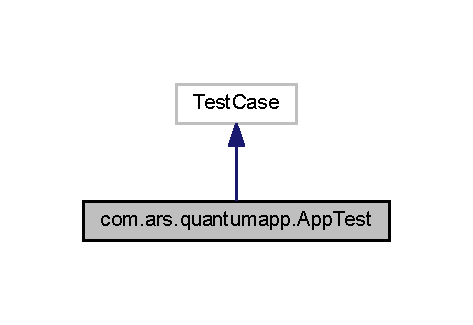
\includegraphics[width=227pt]{classcom_1_1ars_1_1quantumapp_1_1_app_test__inherit__graph}
\end{center}
\end{figure}


Collaboration diagram for com.\+ars.\+quantumapp.\+App\+Test\+:\nopagebreak
\begin{figure}[H]
\begin{center}
\leavevmode
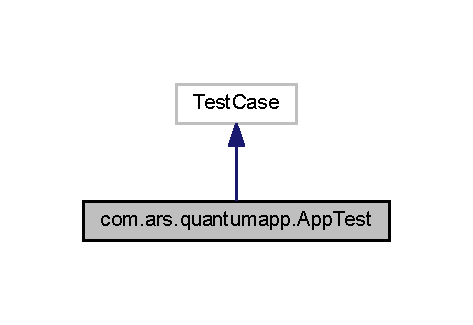
\includegraphics[width=227pt]{classcom_1_1ars_1_1quantumapp_1_1_app_test__coll__graph}
\end{center}
\end{figure}
\subsection*{Public Member Functions}
\begin{DoxyCompactItemize}
\item 
\hyperlink{classcom_1_1ars_1_1quantumapp_1_1_app_test_ad1892904405d218e652b29e79de2de1d}{App\+Test} (String test\+Name)
\item 
void \hyperlink{classcom_1_1ars_1_1quantumapp_1_1_app_test_a37866d2d52dc17cbba459bb947972bdd}{test\+App} ()
\end{DoxyCompactItemize}
\subsection*{Static Public Member Functions}
\begin{DoxyCompactItemize}
\item 
static Test \hyperlink{classcom_1_1ars_1_1quantumapp_1_1_app_test_a59952e08bf166edc6c98639f14442fed}{suite} ()
\end{DoxyCompactItemize}


\subsection{Detailed Description}
Unit test for simple \hyperlink{classcom_1_1ars_1_1quantumapp_1_1_app}{App}. 

\subsection{Constructor \& Destructor Documentation}
\hypertarget{classcom_1_1ars_1_1quantumapp_1_1_app_test_ad1892904405d218e652b29e79de2de1d}{}\label{classcom_1_1ars_1_1quantumapp_1_1_app_test_ad1892904405d218e652b29e79de2de1d} 
\index{com\+::ars\+::quantumapp\+::\+App\+Test@{com\+::ars\+::quantumapp\+::\+App\+Test}!App\+Test@{App\+Test}}
\index{App\+Test@{App\+Test}!com\+::ars\+::quantumapp\+::\+App\+Test@{com\+::ars\+::quantumapp\+::\+App\+Test}}
\subsubsection{\texorpdfstring{App\+Test()}{AppTest()}}
{\footnotesize\ttfamily com.\+ars.\+quantumapp.\+App\+Test.\+App\+Test (\begin{DoxyParamCaption}\item[{String}]{test\+Name }\end{DoxyParamCaption})}

Create the test case


\begin{DoxyParams}{Parameters}
{\em test\+Name} & name of the test case \\
\hline
\end{DoxyParams}


\subsection{Member Function Documentation}
\hypertarget{classcom_1_1ars_1_1quantumapp_1_1_app_test_a59952e08bf166edc6c98639f14442fed}{}\label{classcom_1_1ars_1_1quantumapp_1_1_app_test_a59952e08bf166edc6c98639f14442fed} 
\index{com\+::ars\+::quantumapp\+::\+App\+Test@{com\+::ars\+::quantumapp\+::\+App\+Test}!suite@{suite}}
\index{suite@{suite}!com\+::ars\+::quantumapp\+::\+App\+Test@{com\+::ars\+::quantumapp\+::\+App\+Test}}
\subsubsection{\texorpdfstring{suite()}{suite()}}
{\footnotesize\ttfamily static Test com.\+ars.\+quantumapp.\+App\+Test.\+suite (\begin{DoxyParamCaption}{ }\end{DoxyParamCaption})\hspace{0.3cm}{\ttfamily [static]}}

\begin{DoxyReturn}{Returns}
the suite of tests being tested 
\end{DoxyReturn}
\hypertarget{classcom_1_1ars_1_1quantumapp_1_1_app_test_a37866d2d52dc17cbba459bb947972bdd}{}\label{classcom_1_1ars_1_1quantumapp_1_1_app_test_a37866d2d52dc17cbba459bb947972bdd} 
\index{com\+::ars\+::quantumapp\+::\+App\+Test@{com\+::ars\+::quantumapp\+::\+App\+Test}!test\+App@{test\+App}}
\index{test\+App@{test\+App}!com\+::ars\+::quantumapp\+::\+App\+Test@{com\+::ars\+::quantumapp\+::\+App\+Test}}
\subsubsection{\texorpdfstring{test\+App()}{testApp()}}
{\footnotesize\ttfamily void com.\+ars.\+quantumapp.\+App\+Test.\+test\+App (\begin{DoxyParamCaption}{ }\end{DoxyParamCaption})}

Rigourous Test \+:-\/) 

The documentation for this class was generated from the following file\+:\begin{DoxyCompactItemize}
\item 
C\+:/\+Users/\+Dacian/\+Desktop/\+Quantum/\+Quantum/quantum\+\_\+computing-\/master/quantumapp/src/test/java/com/ars/quantumapp/\hyperlink{_app_test_8java}{App\+Test.\+java}\end{DoxyCompactItemize}

\hypertarget{classcom_1_1ars_1_1circuits_1_1_circuit_factory}{}\section{com.\+ars.\+circuits.\+Circuit\+Factory Class Reference}
\label{classcom_1_1ars_1_1circuits_1_1_circuit_factory}\index{com.\+ars.\+circuits.\+Circuit\+Factory@{com.\+ars.\+circuits.\+Circuit\+Factory}}


Inheritance diagram for com.\+ars.\+circuits.\+Circuit\+Factory\+:
\nopagebreak
\begin{figure}[H]
\begin{center}
\leavevmode
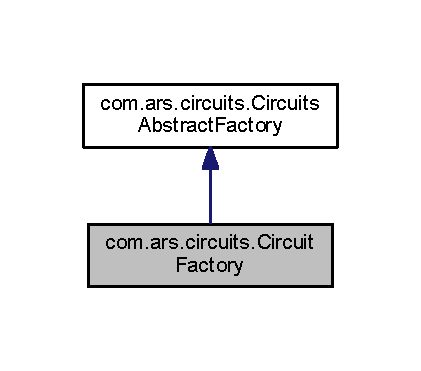
\includegraphics[width=202pt]{classcom_1_1ars_1_1circuits_1_1_circuit_factory__inherit__graph}
\end{center}
\end{figure}


Collaboration diagram for com.\+ars.\+circuits.\+Circuit\+Factory\+:
\nopagebreak
\begin{figure}[H]
\begin{center}
\leavevmode
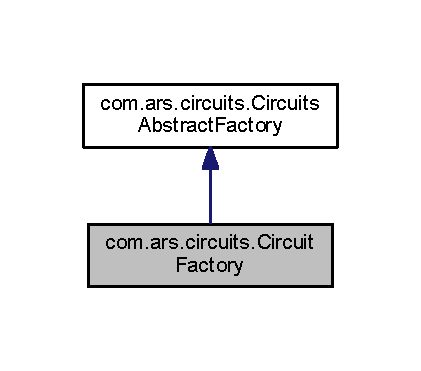
\includegraphics[width=202pt]{classcom_1_1ars_1_1circuits_1_1_circuit_factory__coll__graph}
\end{center}
\end{figure}
\subsection*{Public Member Functions}
\begin{DoxyCompactItemize}
\item 
\hyperlink{interfacecom_1_1ars_1_1circuits_1_1_i_circuit}{I\+Circuit} \hyperlink{classcom_1_1ars_1_1circuits_1_1_circuit_factory_a0546784d697bdf29e7841c75bb98c8a8}{get\+Circuit} (\hyperlink{enumcom_1_1ars_1_1circuits_1_1_circuit_types}{Circuit\+Types} id)
\end{DoxyCompactItemize}


\subsection{Member Function Documentation}
\hypertarget{classcom_1_1ars_1_1circuits_1_1_circuit_factory_a0546784d697bdf29e7841c75bb98c8a8}{}\label{classcom_1_1ars_1_1circuits_1_1_circuit_factory_a0546784d697bdf29e7841c75bb98c8a8} 
\index{com\+::ars\+::circuits\+::\+Circuit\+Factory@{com\+::ars\+::circuits\+::\+Circuit\+Factory}!get\+Circuit@{get\+Circuit}}
\index{get\+Circuit@{get\+Circuit}!com\+::ars\+::circuits\+::\+Circuit\+Factory@{com\+::ars\+::circuits\+::\+Circuit\+Factory}}
\subsubsection{\texorpdfstring{get\+Circuit()}{getCircuit()}}
{\footnotesize\ttfamily \hyperlink{interfacecom_1_1ars_1_1circuits_1_1_i_circuit}{I\+Circuit} com.\+ars.\+circuits.\+Circuit\+Factory.\+get\+Circuit (\begin{DoxyParamCaption}\item[{\hyperlink{enumcom_1_1ars_1_1circuits_1_1_circuit_types}{Circuit\+Types}}]{id }\end{DoxyParamCaption})}



The documentation for this class was generated from the following file\+:\begin{DoxyCompactItemize}
\item 
C\+:/\+Users/\+Dacian/\+Desktop/\+Quantum/\+Quantum/quantum\+\_\+computing-\/master/quantum/src/main/java/com/ars/circuits/\hyperlink{_circuit_factory_8java}{Circuit\+Factory.\+java}\end{DoxyCompactItemize}

\hypertarget{classcom_1_1ars_1_1circuits_1_1_circuit_producer}{}\section{com.\+ars.\+circuits.\+Circuit\+Producer Class Reference}
\label{classcom_1_1ars_1_1circuits_1_1_circuit_producer}\index{com.\+ars.\+circuits.\+Circuit\+Producer@{com.\+ars.\+circuits.\+Circuit\+Producer}}
\subsection*{Static Public Member Functions}
\begin{DoxyCompactItemize}
\item 
static \hyperlink{classcom_1_1ars_1_1circuits_1_1_circuits_abstract_factory}{Circuits\+Abstract\+Factory} \hyperlink{classcom_1_1ars_1_1circuits_1_1_circuit_producer_a309e58fbb248b354abc746f9a82233eb}{get\+Circuit\+Factory} ()
\end{DoxyCompactItemize}


\subsection{Member Function Documentation}
\hypertarget{classcom_1_1ars_1_1circuits_1_1_circuit_producer_a309e58fbb248b354abc746f9a82233eb}{}\label{classcom_1_1ars_1_1circuits_1_1_circuit_producer_a309e58fbb248b354abc746f9a82233eb} 
\index{com\+::ars\+::circuits\+::\+Circuit\+Producer@{com\+::ars\+::circuits\+::\+Circuit\+Producer}!get\+Circuit\+Factory@{get\+Circuit\+Factory}}
\index{get\+Circuit\+Factory@{get\+Circuit\+Factory}!com\+::ars\+::circuits\+::\+Circuit\+Producer@{com\+::ars\+::circuits\+::\+Circuit\+Producer}}
\subsubsection{\texorpdfstring{get\+Circuit\+Factory()}{getCircuitFactory()}}
{\footnotesize\ttfamily static \hyperlink{classcom_1_1ars_1_1circuits_1_1_circuits_abstract_factory}{Circuits\+Abstract\+Factory} com.\+ars.\+circuits.\+Circuit\+Producer.\+get\+Circuit\+Factory (\begin{DoxyParamCaption}{ }\end{DoxyParamCaption})\hspace{0.3cm}{\ttfamily [static]}}



The documentation for this class was generated from the following file\+:\begin{DoxyCompactItemize}
\item 
C\+:/\+Users/\+Dacian/\+Desktop/\+Quantum/\+Quantum/quantum\+\_\+computing-\/master/quantum/src/main/java/com/ars/circuits/\hyperlink{_circuit_producer_8java}{Circuit\+Producer.\+java}\end{DoxyCompactItemize}

\hypertarget{classcom_1_1ars_1_1circuits_1_1_circuits_abstract_factory}{}\section{com.\+ars.\+circuits.\+Circuits\+Abstract\+Factory Class Reference}
\label{classcom_1_1ars_1_1circuits_1_1_circuits_abstract_factory}\index{com.\+ars.\+circuits.\+Circuits\+Abstract\+Factory@{com.\+ars.\+circuits.\+Circuits\+Abstract\+Factory}}


Inheritance diagram for com.\+ars.\+circuits.\+Circuits\+Abstract\+Factory\+:
\nopagebreak
\begin{figure}[H]
\begin{center}
\leavevmode
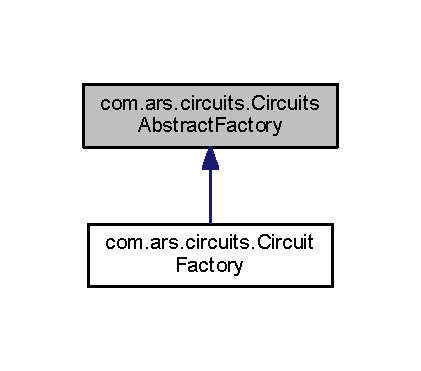
\includegraphics[width=202pt]{classcom_1_1ars_1_1circuits_1_1_circuits_abstract_factory__inherit__graph}
\end{center}
\end{figure}
\subsection*{Public Member Functions}
\begin{DoxyCompactItemize}
\item 
abstract \hyperlink{interfacecom_1_1ars_1_1circuits_1_1_i_circuit}{I\+Circuit} \hyperlink{classcom_1_1ars_1_1circuits_1_1_circuits_abstract_factory_a626deadf5570c3d0e23c2b57627578e9}{get\+Circuit} (\hyperlink{enumcom_1_1ars_1_1circuits_1_1_circuit_types}{Circuit\+Types} id)
\end{DoxyCompactItemize}


\subsection{Member Function Documentation}
\hypertarget{classcom_1_1ars_1_1circuits_1_1_circuits_abstract_factory_a626deadf5570c3d0e23c2b57627578e9}{}\label{classcom_1_1ars_1_1circuits_1_1_circuits_abstract_factory_a626deadf5570c3d0e23c2b57627578e9} 
\index{com\+::ars\+::circuits\+::\+Circuits\+Abstract\+Factory@{com\+::ars\+::circuits\+::\+Circuits\+Abstract\+Factory}!get\+Circuit@{get\+Circuit}}
\index{get\+Circuit@{get\+Circuit}!com\+::ars\+::circuits\+::\+Circuits\+Abstract\+Factory@{com\+::ars\+::circuits\+::\+Circuits\+Abstract\+Factory}}
\subsubsection{\texorpdfstring{get\+Circuit()}{getCircuit()}}
{\footnotesize\ttfamily abstract \hyperlink{interfacecom_1_1ars_1_1circuits_1_1_i_circuit}{I\+Circuit} com.\+ars.\+circuits.\+Circuits\+Abstract\+Factory.\+get\+Circuit (\begin{DoxyParamCaption}\item[{\hyperlink{enumcom_1_1ars_1_1circuits_1_1_circuit_types}{Circuit\+Types}}]{id }\end{DoxyParamCaption})\hspace{0.3cm}{\ttfamily [abstract]}}

Here is the caller graph for this function\+:
\nopagebreak
\begin{figure}[H]
\begin{center}
\leavevmode
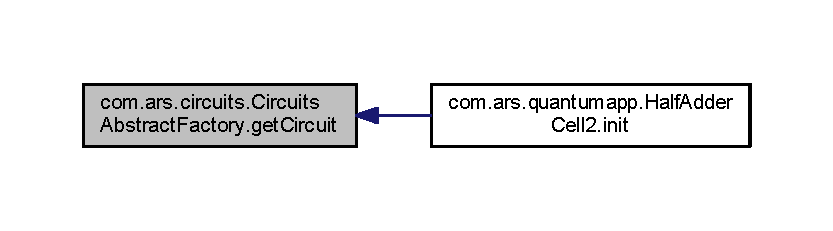
\includegraphics[width=350pt]{classcom_1_1ars_1_1circuits_1_1_circuits_abstract_factory_a626deadf5570c3d0e23c2b57627578e9_icgraph}
\end{center}
\end{figure}


The documentation for this class was generated from the following file\+:\begin{DoxyCompactItemize}
\item 
C\+:/\+Users/\+Dacian/\+Desktop/\+Quantum/\+Quantum/quantum\+\_\+computing-\/master/quantum/src/main/java/com/ars/circuits/\hyperlink{_circuits_abstract_factory_8java}{Circuits\+Abstract\+Factory.\+java}\end{DoxyCompactItemize}

\hypertarget{enumcom_1_1ars_1_1circuits_1_1_circuit_types}{}\section{com.\+ars.\+circuits.\+Circuit\+Types Enum Reference}
\label{enumcom_1_1ars_1_1circuits_1_1_circuit_types}\index{com.\+ars.\+circuits.\+Circuit\+Types@{com.\+ars.\+circuits.\+Circuit\+Types}}
\subsection*{Public Attributes}
\begin{DoxyCompactItemize}
\item 
\hyperlink{enumcom_1_1ars_1_1circuits_1_1_circuit_types_a63e41e3d70dad2b10cc47aeef161755f}{E\+\_\+\+Half\+Adder\+Cell}
\end{DoxyCompactItemize}


\subsection{Member Data Documentation}
\hypertarget{enumcom_1_1ars_1_1circuits_1_1_circuit_types_a63e41e3d70dad2b10cc47aeef161755f}{}\label{enumcom_1_1ars_1_1circuits_1_1_circuit_types_a63e41e3d70dad2b10cc47aeef161755f} 
\index{com\+::ars\+::circuits\+::\+Circuit\+Types@{com\+::ars\+::circuits\+::\+Circuit\+Types}!E\+\_\+\+Half\+Adder\+Cell@{E\+\_\+\+Half\+Adder\+Cell}}
\index{E\+\_\+\+Half\+Adder\+Cell@{E\+\_\+\+Half\+Adder\+Cell}!com\+::ars\+::circuits\+::\+Circuit\+Types@{com\+::ars\+::circuits\+::\+Circuit\+Types}}
\subsubsection{\texorpdfstring{E\+\_\+\+Half\+Adder\+Cell}{E\_HalfAdderCell}}
{\footnotesize\ttfamily com.\+ars.\+circuits.\+Circuit\+Types.\+E\+\_\+\+Half\+Adder\+Cell}



The documentation for this enum was generated from the following file\+:\begin{DoxyCompactItemize}
\item 
C\+:/\+Users/\+Dacian/\+Desktop/\+Quantum/\+Quantum/quantum\+\_\+computing-\/master/quantum/src/main/java/com/ars/circuits/\hyperlink{_circuit_types_8java}{Circuit\+Types.\+java}\end{DoxyCompactItemize}

\hypertarget{classcom_1_1ars_1_1gates_1_1_c_not_gate}{}\section{com.\+ars.\+gates.\+C\+Not\+Gate Class Reference}
\label{classcom_1_1ars_1_1gates_1_1_c_not_gate}\index{com.\+ars.\+gates.\+C\+Not\+Gate@{com.\+ars.\+gates.\+C\+Not\+Gate}}


Inheritance diagram for com.\+ars.\+gates.\+C\+Not\+Gate\+:\nopagebreak
\begin{figure}[H]
\begin{center}
\leavevmode
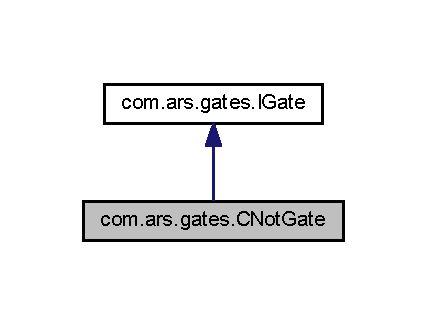
\includegraphics[width=205pt]{classcom_1_1ars_1_1gates_1_1_c_not_gate__inherit__graph}
\end{center}
\end{figure}


Collaboration diagram for com.\+ars.\+gates.\+C\+Not\+Gate\+:\nopagebreak
\begin{figure}[H]
\begin{center}
\leavevmode
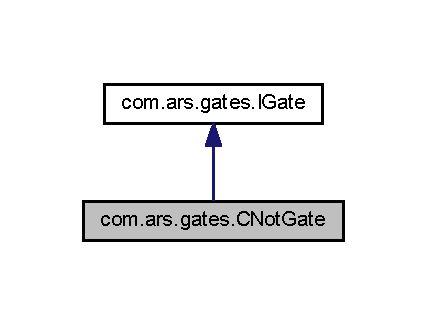
\includegraphics[width=205pt]{classcom_1_1ars_1_1gates_1_1_c_not_gate__coll__graph}
\end{center}
\end{figure}
\subsection*{Public Member Functions}
\begin{DoxyCompactItemize}
\item 
double \mbox{[}$\,$\mbox{]}\mbox{[}$\,$\mbox{]} \hyperlink{classcom_1_1ars_1_1gates_1_1_c_not_gate_a3a78f3ef3d7a418a51b3fabc46954ec5}{get\+Unitary\+Matrix} ()
\end{DoxyCompactItemize}


\subsection{Detailed Description}
Implements the C\+N\+OT Gate 

\subsection{Member Function Documentation}
\hypertarget{classcom_1_1ars_1_1gates_1_1_c_not_gate_a3a78f3ef3d7a418a51b3fabc46954ec5}{}\label{classcom_1_1ars_1_1gates_1_1_c_not_gate_a3a78f3ef3d7a418a51b3fabc46954ec5} 
\index{com\+::ars\+::gates\+::\+C\+Not\+Gate@{com\+::ars\+::gates\+::\+C\+Not\+Gate}!get\+Unitary\+Matrix@{get\+Unitary\+Matrix}}
\index{get\+Unitary\+Matrix@{get\+Unitary\+Matrix}!com\+::ars\+::gates\+::\+C\+Not\+Gate@{com\+::ars\+::gates\+::\+C\+Not\+Gate}}
\subsubsection{\texorpdfstring{get\+Unitary\+Matrix()}{getUnitaryMatrix()}}
{\footnotesize\ttfamily double \mbox{[}$\,$\mbox{]}\mbox{[}$\,$\mbox{]} com.\+ars.\+gates.\+C\+Not\+Gate.\+get\+Unitary\+Matrix (\begin{DoxyParamCaption}{ }\end{DoxyParamCaption})}

Return the 2D array corresponding to a C\+N\+OT gate. \begin{DoxyReturn}{Returns}
double\mbox{[}\mbox{]}\mbox{[}\mbox{]} the corresponding 2D array 
\end{DoxyReturn}


Implements \hyperlink{interfacecom_1_1ars_1_1gates_1_1_i_gate_a6a940b3a6940cd97429aa211143121cb}{com.\+ars.\+gates.\+I\+Gate}.



The documentation for this class was generated from the following file\+:\begin{DoxyCompactItemize}
\item 
C\+:/\+Users/\+Dacian/\+Desktop/\+Quantum/\+Quantum/quantum\+\_\+computing-\/master/quantum/src/main/java/com/ars/gates/\hyperlink{_c_not_gate_8java}{C\+Not\+Gate.\+java}\end{DoxyCompactItemize}

\hypertarget{classcom_1_1ars_1_1complexnumbers_1_1_complex_math}{}\section{com.\+ars.\+complexnumbers.\+Complex\+Math Class Reference}
\label{classcom_1_1ars_1_1complexnumbers_1_1_complex_math}\index{com.\+ars.\+complexnumbers.\+Complex\+Math@{com.\+ars.\+complexnumbers.\+Complex\+Math}}
\subsection*{Static Public Member Functions}
\begin{DoxyCompactItemize}
\item 
static \hyperlink{classcom_1_1ars_1_1complexnumbers_1_1_complex_number}{Complex\+Number} \hyperlink{classcom_1_1ars_1_1complexnumbers_1_1_complex_math_a5d0a70f5fa36204c59c62f3d63391c25}{add} (\hyperlink{classcom_1_1ars_1_1complexnumbers_1_1_complex_number}{Complex\+Number} z1, \hyperlink{classcom_1_1ars_1_1complexnumbers_1_1_complex_number}{Complex\+Number} z2)
\item 
static \hyperlink{classcom_1_1ars_1_1complexnumbers_1_1_complex_number}{Complex\+Number} \hyperlink{classcom_1_1ars_1_1complexnumbers_1_1_complex_math_a0283601c9ce6efc0636468ee5e65f299}{multiply} (\hyperlink{classcom_1_1ars_1_1complexnumbers_1_1_complex_number}{Complex\+Number} z1, \hyperlink{classcom_1_1ars_1_1complexnumbers_1_1_complex_number}{Complex\+Number} z2)
\item 
static \hyperlink{classcom_1_1ars_1_1complexnumbers_1_1_complex_number}{Complex\+Number} \hyperlink{classcom_1_1ars_1_1complexnumbers_1_1_complex_math_a2a8bfbcea23cec290cc91c8eeb9ab4fc}{subtract} (\hyperlink{classcom_1_1ars_1_1complexnumbers_1_1_complex_number}{Complex\+Number} z1, \hyperlink{classcom_1_1ars_1_1complexnumbers_1_1_complex_number}{Complex\+Number} z2)
\item 
static \hyperlink{classcom_1_1ars_1_1complexnumbers_1_1_complex_number}{Complex\+Number} \hyperlink{classcom_1_1ars_1_1complexnumbers_1_1_complex_math_a390a771ed2ef544949621be5375c806a}{divide} (\hyperlink{classcom_1_1ars_1_1complexnumbers_1_1_complex_number}{Complex\+Number} z1, \hyperlink{classcom_1_1ars_1_1complexnumbers_1_1_complex_number}{Complex\+Number} z2)
\item 
static \hyperlink{classcom_1_1ars_1_1complexnumbers_1_1_complex_number}{Complex\+Number} \hyperlink{classcom_1_1ars_1_1complexnumbers_1_1_complex_math_aed293397f1ec0c1dda82589b436388c3}{conjugate} (\hyperlink{classcom_1_1ars_1_1complexnumbers_1_1_complex_number}{Complex\+Number} z)
\item 
static double \hyperlink{classcom_1_1ars_1_1complexnumbers_1_1_complex_math_a1ffa4f4678b201779a1ac8212fc93e05}{mod} (\hyperlink{classcom_1_1ars_1_1complexnumbers_1_1_complex_number}{Complex\+Number} z)
\item 
static \hyperlink{classcom_1_1ars_1_1complexnumbers_1_1_complex_number}{Complex\+Number} \hyperlink{classcom_1_1ars_1_1complexnumbers_1_1_complex_math_ae8123eba1e8ecec75ed3d9fd05410ca2}{square} (\hyperlink{classcom_1_1ars_1_1complexnumbers_1_1_complex_number}{Complex\+Number} z)
\item 
static \hyperlink{classcom_1_1ars_1_1complexnumbers_1_1_complex_number}{Complex\+Number} \hyperlink{classcom_1_1ars_1_1complexnumbers_1_1_complex_math_a9c1d532e50ed32d01ccdb34d85e8765d}{sin} (\hyperlink{classcom_1_1ars_1_1complexnumbers_1_1_complex_number}{Complex\+Number} z)
\item 
static \hyperlink{classcom_1_1ars_1_1complexnumbers_1_1_complex_number}{Complex\+Number} \hyperlink{classcom_1_1ars_1_1complexnumbers_1_1_complex_math_a0ef9a0fc1769a14c5f81f89866643f19}{cos} (\hyperlink{classcom_1_1ars_1_1complexnumbers_1_1_complex_number}{Complex\+Number} z)
\item 
static \hyperlink{classcom_1_1ars_1_1complexnumbers_1_1_complex_number}{Complex\+Number} \hyperlink{classcom_1_1ars_1_1complexnumbers_1_1_complex_math_af260af539eaec79d57b7e5363bda686e}{tan} (\hyperlink{classcom_1_1ars_1_1complexnumbers_1_1_complex_number}{Complex\+Number} z)
\item 
static \hyperlink{classcom_1_1ars_1_1complexnumbers_1_1_complex_number}{Complex\+Number} \hyperlink{classcom_1_1ars_1_1complexnumbers_1_1_complex_math_a9a15203fe621aaa3738dd41d19b70b5f}{exp} (\hyperlink{classcom_1_1ars_1_1complexnumbers_1_1_complex_number}{Complex\+Number} z)
\item 
static \hyperlink{classcom_1_1ars_1_1complexnumbers_1_1_complex_number}{Complex\+Number} \hyperlink{classcom_1_1ars_1_1complexnumbers_1_1_complex_math_a0e31bcd8237beabdee3f1480e8667d83}{pow} (\hyperlink{classcom_1_1ars_1_1complexnumbers_1_1_complex_number}{Complex\+Number} z, int power)
\item 
static \hyperlink{classcom_1_1ars_1_1complexnumbers_1_1_complex_number}{Complex\+Number} \hyperlink{classcom_1_1ars_1_1complexnumbers_1_1_complex_math_a06897e69e7c59bf707851f4a502d11b8}{inverse} (\hyperlink{classcom_1_1ars_1_1complexnumbers_1_1_complex_number}{Complex\+Number} z)
\item 
static \hyperlink{classcom_1_1ars_1_1complexnumbers_1_1_complex_number}{Complex\+Number} \hyperlink{classcom_1_1ars_1_1complexnumbers_1_1_complex_math_aea5e553e5a5e3e519df64cb155699198}{multiply} (\hyperlink{classcom_1_1ars_1_1complexnumbers_1_1_complex_number}{Complex\+Number} z, double constant)
\item 
static \hyperlink{classcom_1_1ars_1_1complexnumbers_1_1_complex_number}{Complex\+Number} \hyperlink{classcom_1_1ars_1_1complexnumbers_1_1_complex_math_ac40f506def2684820fa0c85c6672f5a3}{add} (\hyperlink{classcom_1_1ars_1_1complexnumbers_1_1_complex_number}{Complex\+Number} z, double constant)
\item 
static \hyperlink{classcom_1_1ars_1_1complexnumbers_1_1_complex_number}{Complex\+Number} \hyperlink{classcom_1_1ars_1_1complexnumbers_1_1_complex_math_a8ec234a476d41f2f32113eb13a0f7630}{subtract} (\hyperlink{classcom_1_1ars_1_1complexnumbers_1_1_complex_number}{Complex\+Number} z, double constant)
\item 
static \hyperlink{classcom_1_1ars_1_1complexnumbers_1_1_complex_number}{Complex\+Number} \hyperlink{classcom_1_1ars_1_1complexnumbers_1_1_complex_math_aeca04302a95a0a22e5bd7069455aacf6}{divide} (\hyperlink{classcom_1_1ars_1_1complexnumbers_1_1_complex_number}{Complex\+Number} z, double constant)
\end{DoxyCompactItemize}


\subsection{Detailed Description}
\subsection*{\hyperlink{classcom_1_1ars_1_1complexnumbers_1_1_complex_math}{Complex\+Math}}

\hyperlink{classcom_1_1ars_1_1complexnumbers_1_1_complex_math}{Complex\+Math} implements the basic operations that can be performed on complex numbers.

\begin{DoxyAuthor}{Author}
Mihai Seba 
\end{DoxyAuthor}
\begin{DoxyVersion}{Version}
1.\+0 
\end{DoxyVersion}


\subsection{Member Function Documentation}
\hypertarget{classcom_1_1ars_1_1complexnumbers_1_1_complex_math_a5d0a70f5fa36204c59c62f3d63391c25}{}\label{classcom_1_1ars_1_1complexnumbers_1_1_complex_math_a5d0a70f5fa36204c59c62f3d63391c25} 
\index{com\+::ars\+::complexnumbers\+::\+Complex\+Math@{com\+::ars\+::complexnumbers\+::\+Complex\+Math}!add@{add}}
\index{add@{add}!com\+::ars\+::complexnumbers\+::\+Complex\+Math@{com\+::ars\+::complexnumbers\+::\+Complex\+Math}}
\subsubsection{\texorpdfstring{add()}{add()}\hspace{0.1cm}{\footnotesize\ttfamily [1/2]}}
{\footnotesize\ttfamily static \hyperlink{classcom_1_1ars_1_1complexnumbers_1_1_complex_number}{Complex\+Number} com.\+ars.\+complexnumbers.\+Complex\+Math.\+add (\begin{DoxyParamCaption}\item[{\hyperlink{classcom_1_1ars_1_1complexnumbers_1_1_complex_number}{Complex\+Number}}]{z1,  }\item[{\hyperlink{classcom_1_1ars_1_1complexnumbers_1_1_complex_number}{Complex\+Number}}]{z2 }\end{DoxyParamCaption})\hspace{0.3cm}{\ttfamily [static]}}

Performs the addition of two complex numbers. 
\begin{DoxyParams}{Parameters}
{\em z1} & first complex number \\
\hline
{\em z2} & second complex number \\
\hline
\end{DoxyParams}
\begin{DoxyReturn}{Returns}
the sum of the two complex numbers, z1 and z2, z3=z1+z2 
\end{DoxyReturn}
Here is the call graph for this function\+:\nopagebreak
\begin{figure}[H]
\begin{center}
\leavevmode
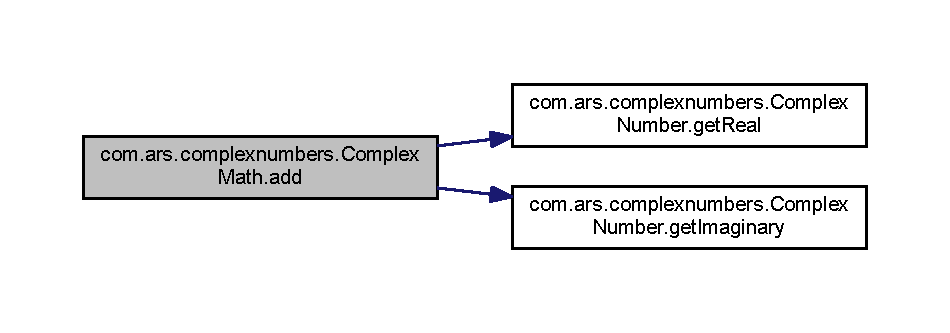
\includegraphics[width=350pt]{classcom_1_1ars_1_1complexnumbers_1_1_complex_math_a5d0a70f5fa36204c59c62f3d63391c25_cgraph}
\end{center}
\end{figure}
Here is the caller graph for this function\+:\nopagebreak
\begin{figure}[H]
\begin{center}
\leavevmode
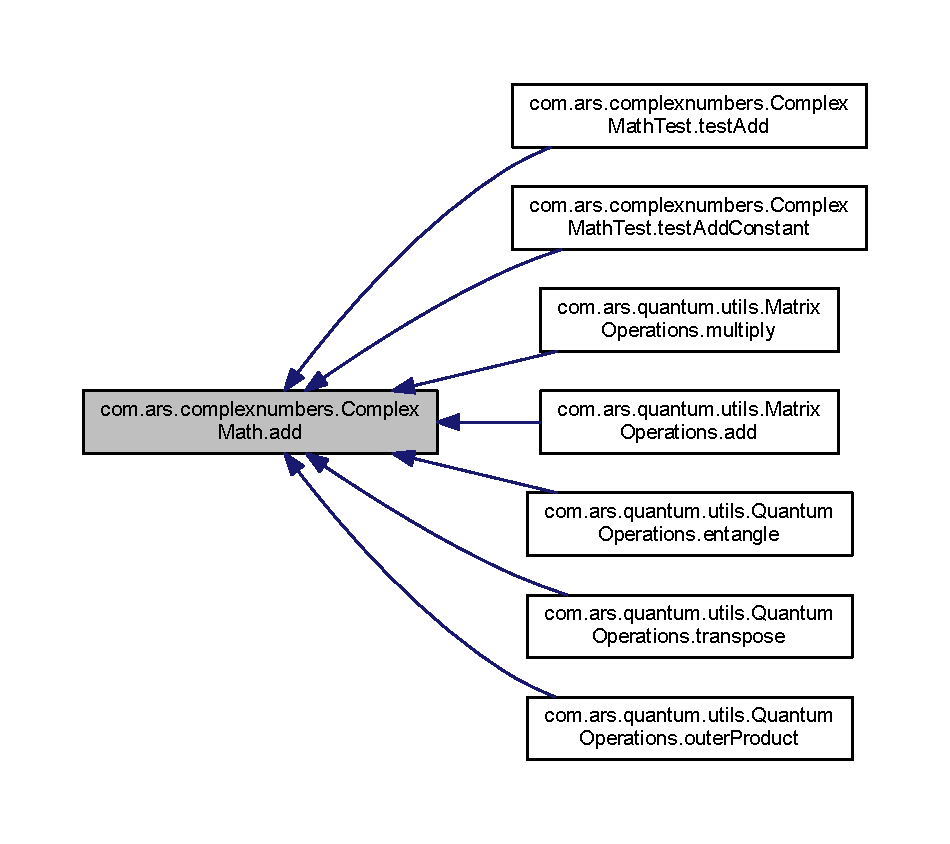
\includegraphics[width=350pt]{classcom_1_1ars_1_1complexnumbers_1_1_complex_math_a5d0a70f5fa36204c59c62f3d63391c25_icgraph}
\end{center}
\end{figure}
\hypertarget{classcom_1_1ars_1_1complexnumbers_1_1_complex_math_ac40f506def2684820fa0c85c6672f5a3}{}\label{classcom_1_1ars_1_1complexnumbers_1_1_complex_math_ac40f506def2684820fa0c85c6672f5a3} 
\index{com\+::ars\+::complexnumbers\+::\+Complex\+Math@{com\+::ars\+::complexnumbers\+::\+Complex\+Math}!add@{add}}
\index{add@{add}!com\+::ars\+::complexnumbers\+::\+Complex\+Math@{com\+::ars\+::complexnumbers\+::\+Complex\+Math}}
\subsubsection{\texorpdfstring{add()}{add()}\hspace{0.1cm}{\footnotesize\ttfamily [2/2]}}
{\footnotesize\ttfamily static \hyperlink{classcom_1_1ars_1_1complexnumbers_1_1_complex_number}{Complex\+Number} com.\+ars.\+complexnumbers.\+Complex\+Math.\+add (\begin{DoxyParamCaption}\item[{\hyperlink{classcom_1_1ars_1_1complexnumbers_1_1_complex_number}{Complex\+Number}}]{z,  }\item[{double}]{constant }\end{DoxyParamCaption})\hspace{0.3cm}{\ttfamily [static]}}

Performs the addition of a complex number with a double. 
\begin{DoxyParams}{Parameters}
{\em z} & complex number \\
\hline
{\em constant} & double number \\
\hline
\end{DoxyParams}
\begin{DoxyReturn}{Returns}
the result of addition. 
\end{DoxyReturn}
Here is the call graph for this function\+:\nopagebreak
\begin{figure}[H]
\begin{center}
\leavevmode
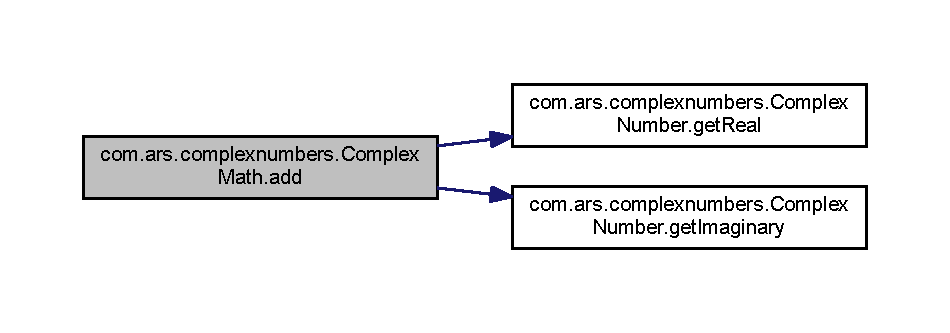
\includegraphics[width=350pt]{classcom_1_1ars_1_1complexnumbers_1_1_complex_math_ac40f506def2684820fa0c85c6672f5a3_cgraph}
\end{center}
\end{figure}
\hypertarget{classcom_1_1ars_1_1complexnumbers_1_1_complex_math_aed293397f1ec0c1dda82589b436388c3}{}\label{classcom_1_1ars_1_1complexnumbers_1_1_complex_math_aed293397f1ec0c1dda82589b436388c3} 
\index{com\+::ars\+::complexnumbers\+::\+Complex\+Math@{com\+::ars\+::complexnumbers\+::\+Complex\+Math}!conjugate@{conjugate}}
\index{conjugate@{conjugate}!com\+::ars\+::complexnumbers\+::\+Complex\+Math@{com\+::ars\+::complexnumbers\+::\+Complex\+Math}}
\subsubsection{\texorpdfstring{conjugate()}{conjugate()}}
{\footnotesize\ttfamily static \hyperlink{classcom_1_1ars_1_1complexnumbers_1_1_complex_number}{Complex\+Number} com.\+ars.\+complexnumbers.\+Complex\+Math.\+conjugate (\begin{DoxyParamCaption}\item[{\hyperlink{classcom_1_1ars_1_1complexnumbers_1_1_complex_number}{Complex\+Number}}]{z }\end{DoxyParamCaption})\hspace{0.3cm}{\ttfamily [static]}}

Calculates the complex conjugate of a {\ttfamily \hyperlink{classcom_1_1ars_1_1complexnumbers_1_1_complex_number}{Complex\+Number}}. 
\begin{DoxyParams}{Parameters}
{\em z} & the input complex number \\
\hline
\end{DoxyParams}
\begin{DoxyReturn}{Returns}
the complex conjugate number of z 
\end{DoxyReturn}
Here is the call graph for this function\+:\nopagebreak
\begin{figure}[H]
\begin{center}
\leavevmode
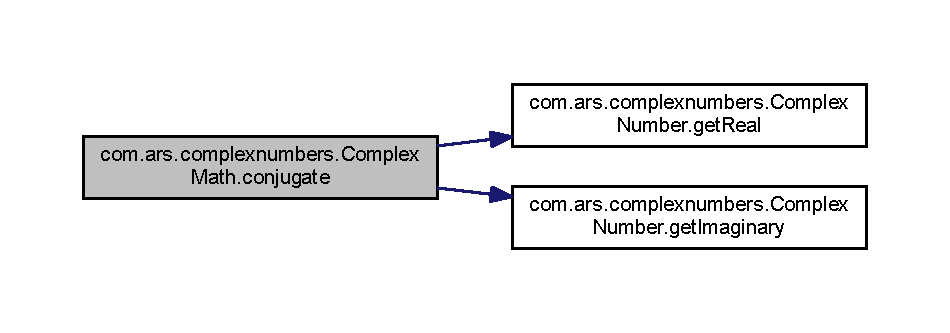
\includegraphics[width=350pt]{classcom_1_1ars_1_1complexnumbers_1_1_complex_math_aed293397f1ec0c1dda82589b436388c3_cgraph}
\end{center}
\end{figure}
Here is the caller graph for this function\+:
\nopagebreak
\begin{figure}[H]
\begin{center}
\leavevmode
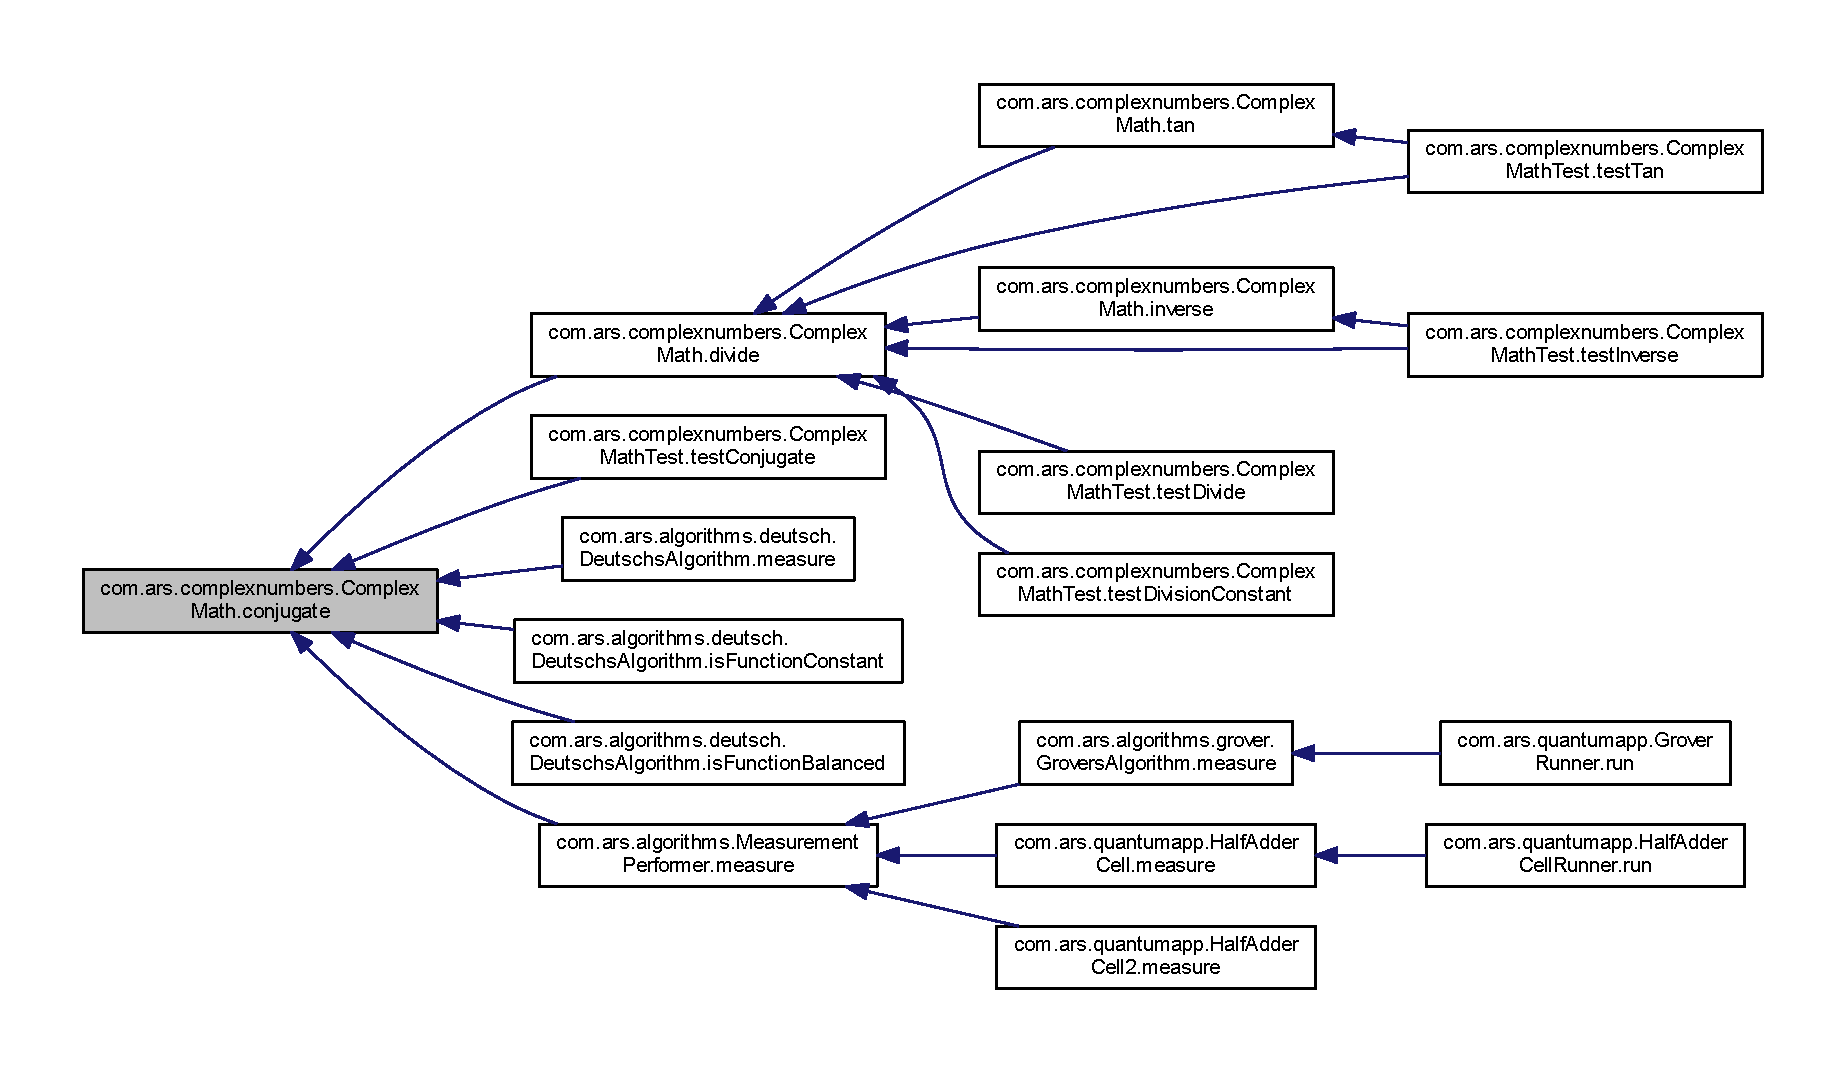
\includegraphics[width=350pt]{classcom_1_1ars_1_1complexnumbers_1_1_complex_math_aed293397f1ec0c1dda82589b436388c3_icgraph}
\end{center}
\end{figure}
\hypertarget{classcom_1_1ars_1_1complexnumbers_1_1_complex_math_a0ef9a0fc1769a14c5f81f89866643f19}{}\label{classcom_1_1ars_1_1complexnumbers_1_1_complex_math_a0ef9a0fc1769a14c5f81f89866643f19} 
\index{com\+::ars\+::complexnumbers\+::\+Complex\+Math@{com\+::ars\+::complexnumbers\+::\+Complex\+Math}!cos@{cos}}
\index{cos@{cos}!com\+::ars\+::complexnumbers\+::\+Complex\+Math@{com\+::ars\+::complexnumbers\+::\+Complex\+Math}}
\subsubsection{\texorpdfstring{cos()}{cos()}}
{\footnotesize\ttfamily static \hyperlink{classcom_1_1ars_1_1complexnumbers_1_1_complex_number}{Complex\+Number} com.\+ars.\+complexnumbers.\+Complex\+Math.\+cos (\begin{DoxyParamCaption}\item[{\hyperlink{classcom_1_1ars_1_1complexnumbers_1_1_complex_number}{Complex\+Number}}]{z }\end{DoxyParamCaption})\hspace{0.3cm}{\ttfamily [static]}}

Calculates the cosine of the {\ttfamily \hyperlink{classcom_1_1ars_1_1complexnumbers_1_1_complex_number}{Complex\+Number}} 
\begin{DoxyParams}{Parameters}
{\em z} & the input complex number \\
\hline
\end{DoxyParams}
\begin{DoxyReturn}{Returns}
return a {\ttfamily \hyperlink{classcom_1_1ars_1_1complexnumbers_1_1_complex_number}{Complex\+Number}} which is cosine of z 
\end{DoxyReturn}
Here is the call graph for this function\+:
\nopagebreak
\begin{figure}[H]
\begin{center}
\leavevmode
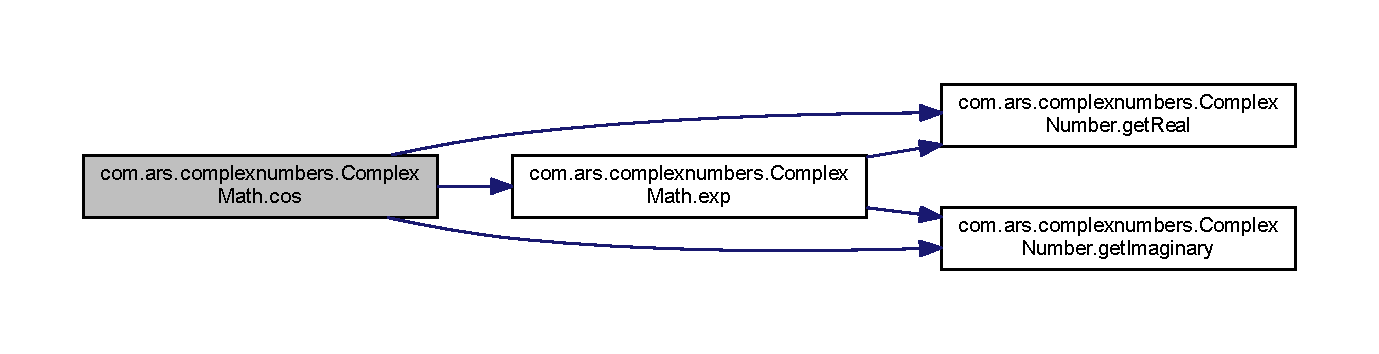
\includegraphics[width=350pt]{classcom_1_1ars_1_1complexnumbers_1_1_complex_math_a0ef9a0fc1769a14c5f81f89866643f19_cgraph}
\end{center}
\end{figure}
Here is the caller graph for this function\+:
\nopagebreak
\begin{figure}[H]
\begin{center}
\leavevmode
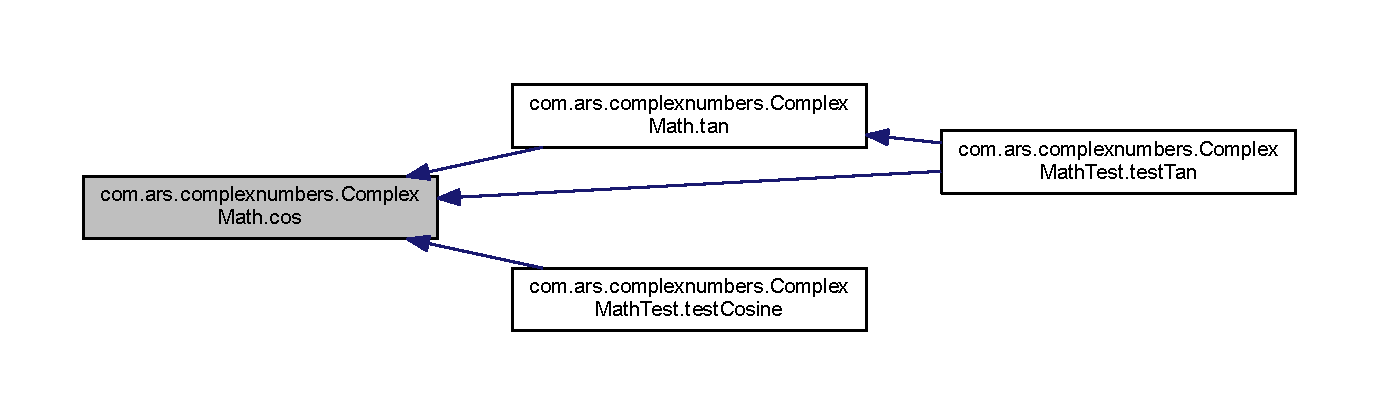
\includegraphics[width=350pt]{classcom_1_1ars_1_1complexnumbers_1_1_complex_math_a0ef9a0fc1769a14c5f81f89866643f19_icgraph}
\end{center}
\end{figure}
\hypertarget{classcom_1_1ars_1_1complexnumbers_1_1_complex_math_a390a771ed2ef544949621be5375c806a}{}\label{classcom_1_1ars_1_1complexnumbers_1_1_complex_math_a390a771ed2ef544949621be5375c806a} 
\index{com\+::ars\+::complexnumbers\+::\+Complex\+Math@{com\+::ars\+::complexnumbers\+::\+Complex\+Math}!divide@{divide}}
\index{divide@{divide}!com\+::ars\+::complexnumbers\+::\+Complex\+Math@{com\+::ars\+::complexnumbers\+::\+Complex\+Math}}
\subsubsection{\texorpdfstring{divide()}{divide()}\hspace{0.1cm}{\footnotesize\ttfamily [1/2]}}
{\footnotesize\ttfamily static \hyperlink{classcom_1_1ars_1_1complexnumbers_1_1_complex_number}{Complex\+Number} com.\+ars.\+complexnumbers.\+Complex\+Math.\+divide (\begin{DoxyParamCaption}\item[{\hyperlink{classcom_1_1ars_1_1complexnumbers_1_1_complex_number}{Complex\+Number}}]{z1,  }\item[{\hyperlink{classcom_1_1ars_1_1complexnumbers_1_1_complex_number}{Complex\+Number}}]{z2 }\end{DoxyParamCaption})\hspace{0.3cm}{\ttfamily [static]}}

Performs the division of two complex numbers. 
\begin{DoxyParams}{Parameters}
{\em z1} & first complex number \\
\hline
{\em z2} & second complex number \\
\hline
\end{DoxyParams}
\begin{DoxyReturn}{Returns}
the result of division, z1 and z2, z3=z1/z2 
\end{DoxyReturn}
Here is the call graph for this function\+:
\nopagebreak
\begin{figure}[H]
\begin{center}
\leavevmode
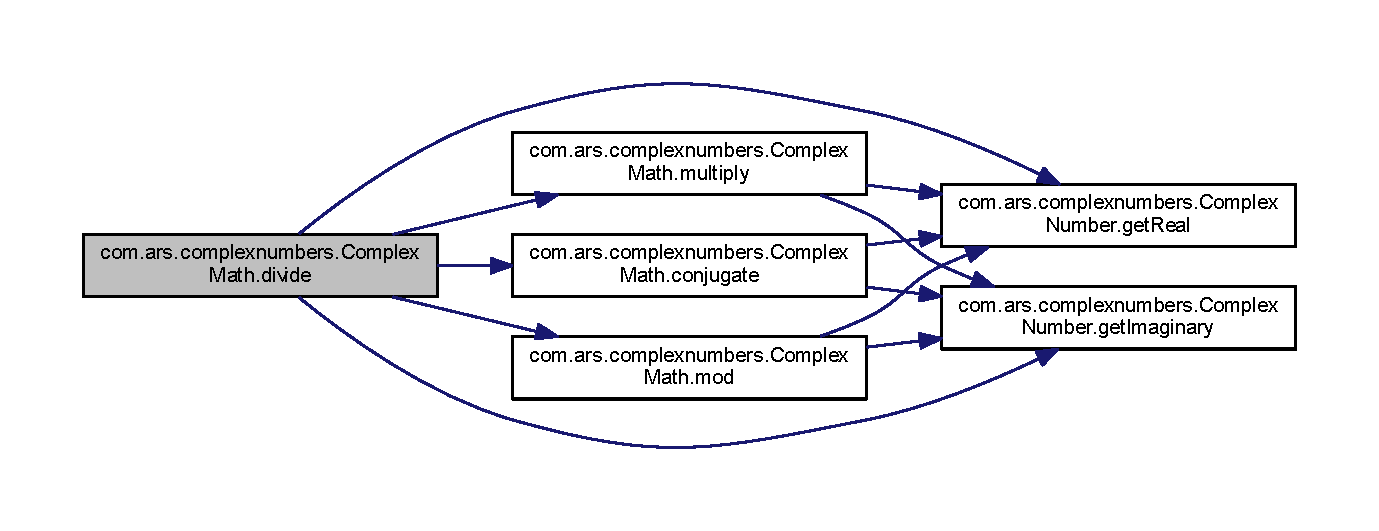
\includegraphics[width=350pt]{classcom_1_1ars_1_1complexnumbers_1_1_complex_math_a390a771ed2ef544949621be5375c806a_cgraph}
\end{center}
\end{figure}
Here is the caller graph for this function\+:
\nopagebreak
\begin{figure}[H]
\begin{center}
\leavevmode
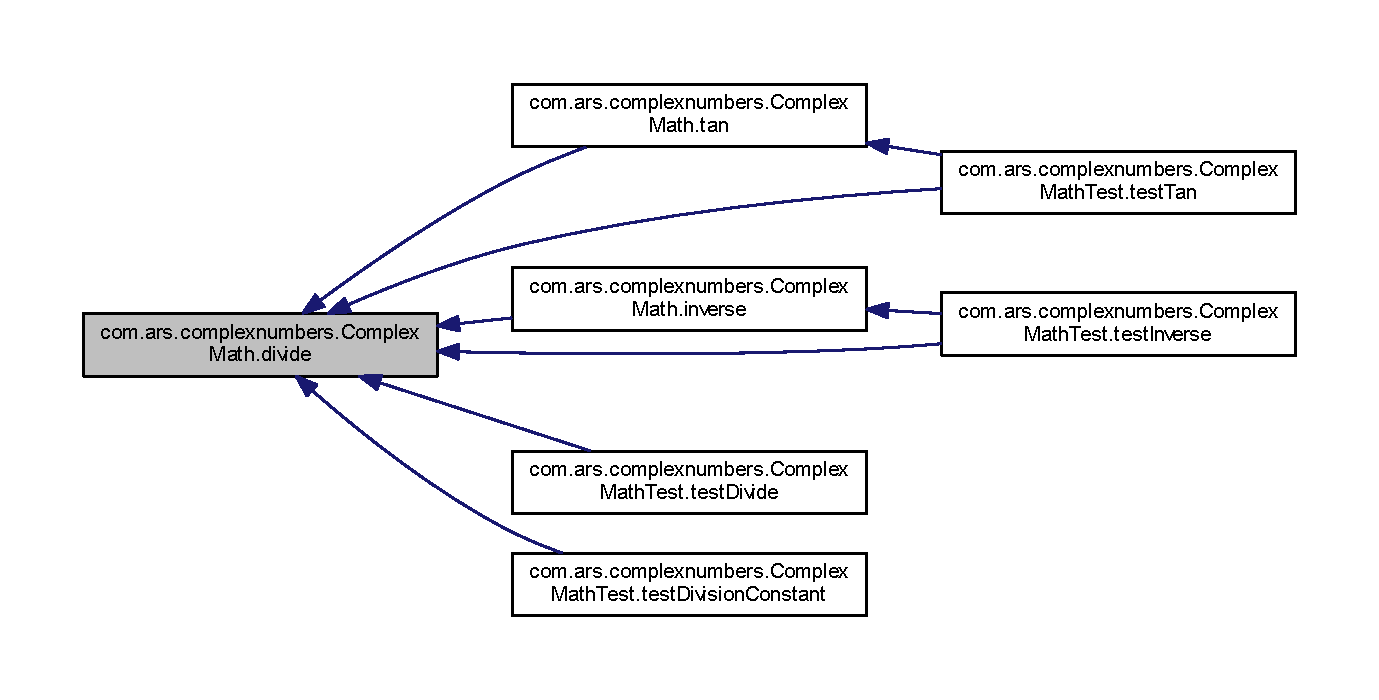
\includegraphics[width=350pt]{classcom_1_1ars_1_1complexnumbers_1_1_complex_math_a390a771ed2ef544949621be5375c806a_icgraph}
\end{center}
\end{figure}
\hypertarget{classcom_1_1ars_1_1complexnumbers_1_1_complex_math_aeca04302a95a0a22e5bd7069455aacf6}{}\label{classcom_1_1ars_1_1complexnumbers_1_1_complex_math_aeca04302a95a0a22e5bd7069455aacf6} 
\index{com\+::ars\+::complexnumbers\+::\+Complex\+Math@{com\+::ars\+::complexnumbers\+::\+Complex\+Math}!divide@{divide}}
\index{divide@{divide}!com\+::ars\+::complexnumbers\+::\+Complex\+Math@{com\+::ars\+::complexnumbers\+::\+Complex\+Math}}
\subsubsection{\texorpdfstring{divide()}{divide()}\hspace{0.1cm}{\footnotesize\ttfamily [2/2]}}
{\footnotesize\ttfamily static \hyperlink{classcom_1_1ars_1_1complexnumbers_1_1_complex_number}{Complex\+Number} com.\+ars.\+complexnumbers.\+Complex\+Math.\+divide (\begin{DoxyParamCaption}\item[{\hyperlink{classcom_1_1ars_1_1complexnumbers_1_1_complex_number}{Complex\+Number}}]{z,  }\item[{double}]{constant }\end{DoxyParamCaption})\hspace{0.3cm}{\ttfamily [static]}}

Performs the division of a complex number with a double. 
\begin{DoxyParams}{Parameters}
{\em z} & complex number \\
\hline
{\em constant} & double number \\
\hline
\end{DoxyParams}
\begin{DoxyReturn}{Returns}
the result of division. 
\end{DoxyReturn}
Here is the call graph for this function\+:
\nopagebreak
\begin{figure}[H]
\begin{center}
\leavevmode
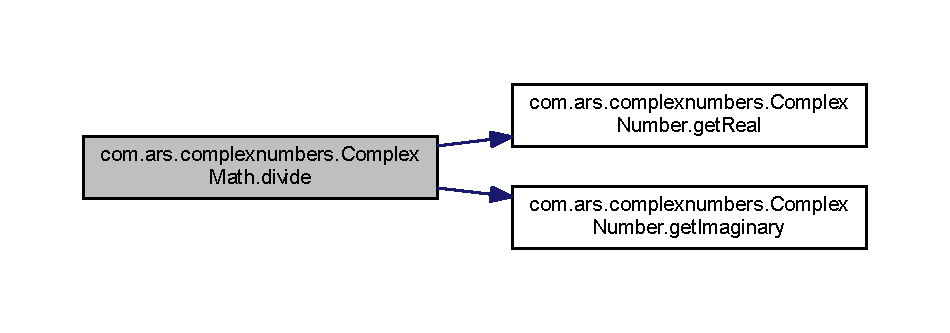
\includegraphics[width=350pt]{classcom_1_1ars_1_1complexnumbers_1_1_complex_math_aeca04302a95a0a22e5bd7069455aacf6_cgraph}
\end{center}
\end{figure}
\hypertarget{classcom_1_1ars_1_1complexnumbers_1_1_complex_math_a9a15203fe621aaa3738dd41d19b70b5f}{}\label{classcom_1_1ars_1_1complexnumbers_1_1_complex_math_a9a15203fe621aaa3738dd41d19b70b5f} 
\index{com\+::ars\+::complexnumbers\+::\+Complex\+Math@{com\+::ars\+::complexnumbers\+::\+Complex\+Math}!exp@{exp}}
\index{exp@{exp}!com\+::ars\+::complexnumbers\+::\+Complex\+Math@{com\+::ars\+::complexnumbers\+::\+Complex\+Math}}
\subsubsection{\texorpdfstring{exp()}{exp()}}
{\footnotesize\ttfamily static \hyperlink{classcom_1_1ars_1_1complexnumbers_1_1_complex_number}{Complex\+Number} com.\+ars.\+complexnumbers.\+Complex\+Math.\+exp (\begin{DoxyParamCaption}\item[{\hyperlink{classcom_1_1ars_1_1complexnumbers_1_1_complex_number}{Complex\+Number}}]{z }\end{DoxyParamCaption})\hspace{0.3cm}{\ttfamily [static]}}

Calculates the exponential of the {\ttfamily \hyperlink{classcom_1_1ars_1_1complexnumbers_1_1_complex_number}{Complex\+Number}} 
\begin{DoxyParams}{Parameters}
{\em z} & the input complex number \\
\hline
\end{DoxyParams}
\begin{DoxyReturn}{Returns}
return a {\ttfamily \hyperlink{classcom_1_1ars_1_1complexnumbers_1_1_complex_number}{Complex\+Number}} which is e$^\wedge$ 
\end{DoxyReturn}
Here is the call graph for this function\+:
\nopagebreak
\begin{figure}[H]
\begin{center}
\leavevmode
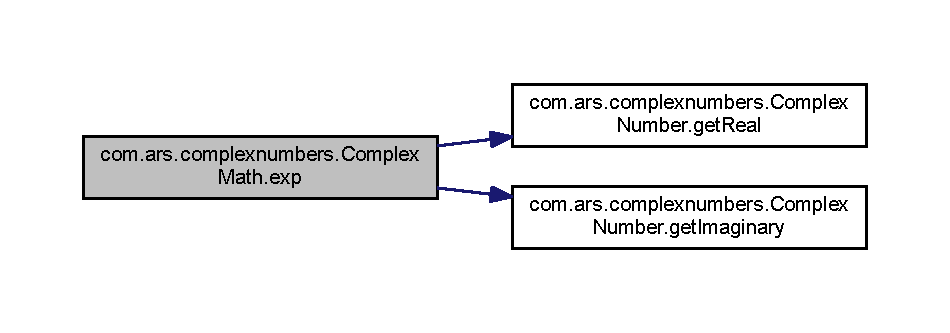
\includegraphics[width=350pt]{classcom_1_1ars_1_1complexnumbers_1_1_complex_math_a9a15203fe621aaa3738dd41d19b70b5f_cgraph}
\end{center}
\end{figure}
Here is the caller graph for this function\+:
\nopagebreak
\begin{figure}[H]
\begin{center}
\leavevmode
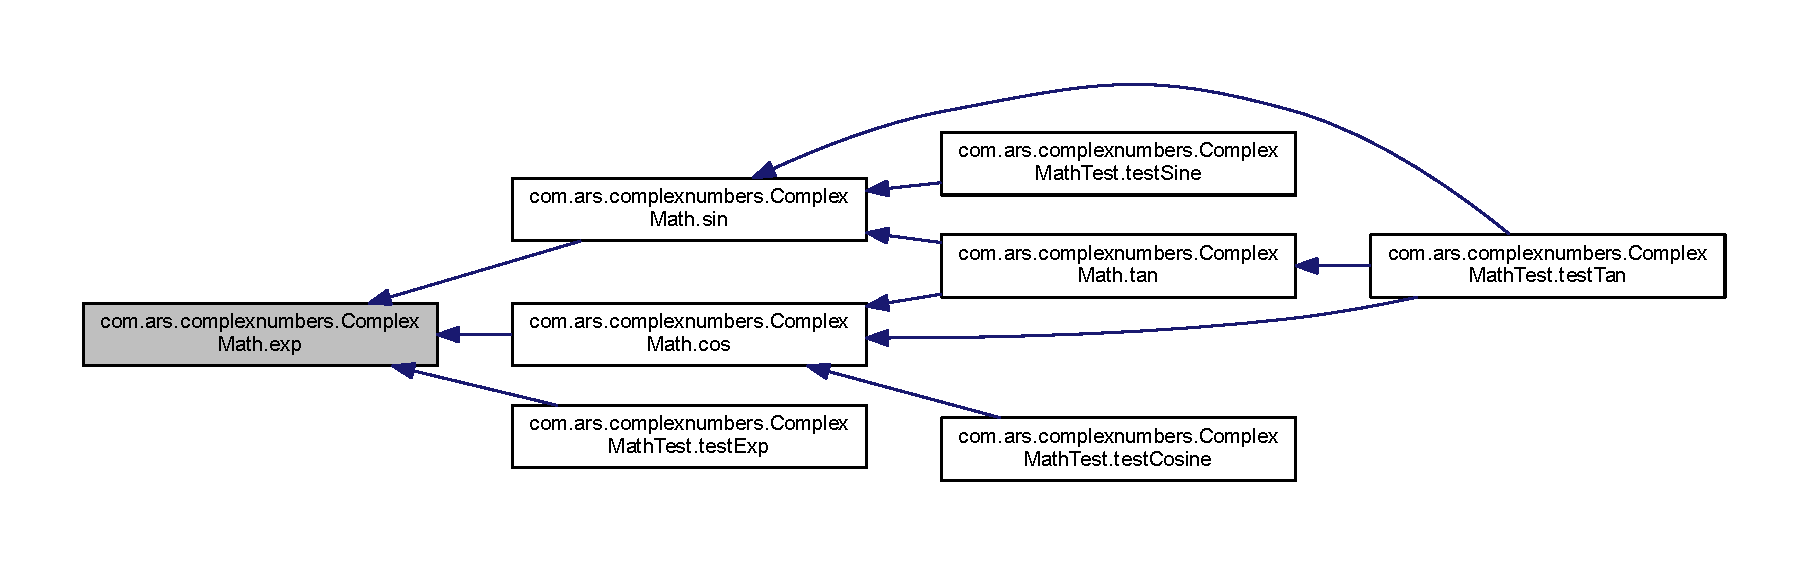
\includegraphics[width=350pt]{classcom_1_1ars_1_1complexnumbers_1_1_complex_math_a9a15203fe621aaa3738dd41d19b70b5f_icgraph}
\end{center}
\end{figure}
\hypertarget{classcom_1_1ars_1_1complexnumbers_1_1_complex_math_a06897e69e7c59bf707851f4a502d11b8}{}\label{classcom_1_1ars_1_1complexnumbers_1_1_complex_math_a06897e69e7c59bf707851f4a502d11b8} 
\index{com\+::ars\+::complexnumbers\+::\+Complex\+Math@{com\+::ars\+::complexnumbers\+::\+Complex\+Math}!inverse@{inverse}}
\index{inverse@{inverse}!com\+::ars\+::complexnumbers\+::\+Complex\+Math@{com\+::ars\+::complexnumbers\+::\+Complex\+Math}}
\subsubsection{\texorpdfstring{inverse()}{inverse()}}
{\footnotesize\ttfamily static \hyperlink{classcom_1_1ars_1_1complexnumbers_1_1_complex_number}{Complex\+Number} com.\+ars.\+complexnumbers.\+Complex\+Math.\+inverse (\begin{DoxyParamCaption}\item[{\hyperlink{classcom_1_1ars_1_1complexnumbers_1_1_complex_number}{Complex\+Number}}]{z }\end{DoxyParamCaption})\hspace{0.3cm}{\ttfamily [static]}}

Calculates the inverse of a {\ttfamily \hyperlink{classcom_1_1ars_1_1complexnumbers_1_1_complex_number}{Complex\+Number}}. 
\begin{DoxyParams}{Parameters}
{\em z} & the input complex number \\
\hline
\end{DoxyParams}
\begin{DoxyReturn}{Returns}
return a {\ttfamily \hyperlink{classcom_1_1ars_1_1complexnumbers_1_1_complex_number}{Complex\+Number}} which is 1/z 
\end{DoxyReturn}
Here is the call graph for this function\+:
\nopagebreak
\begin{figure}[H]
\begin{center}
\leavevmode
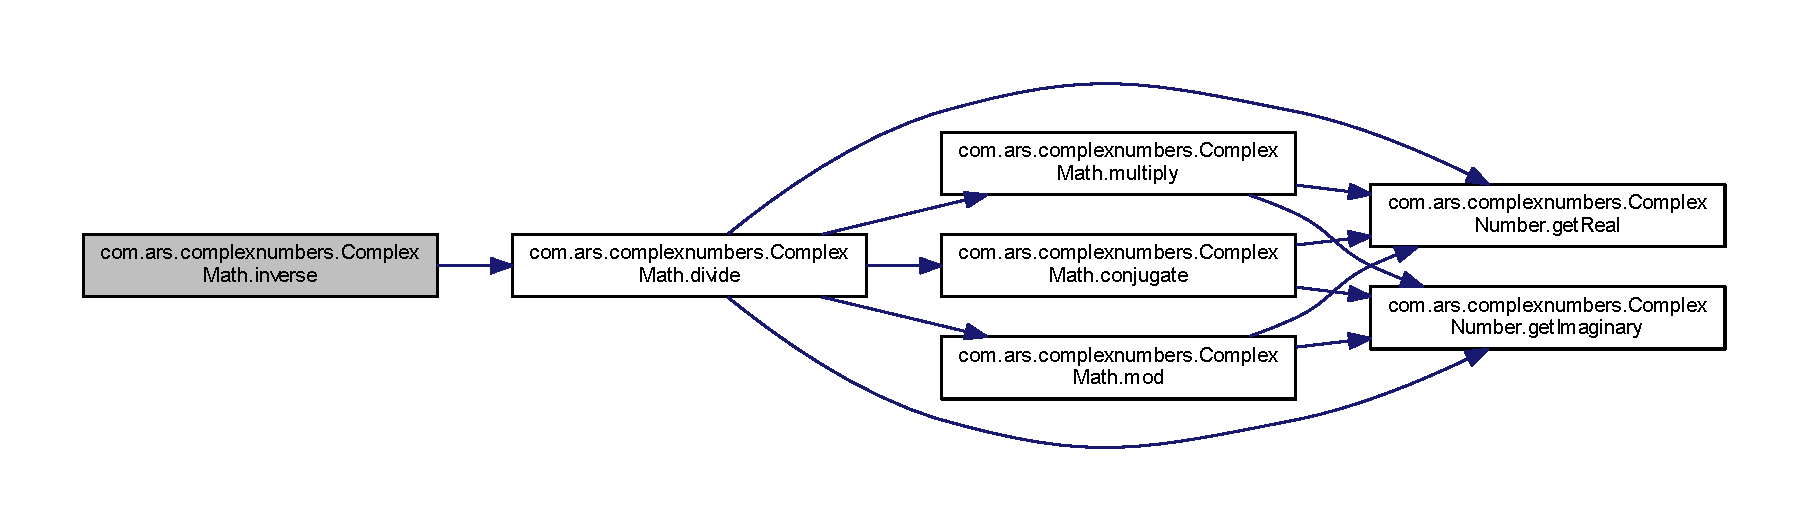
\includegraphics[width=350pt]{classcom_1_1ars_1_1complexnumbers_1_1_complex_math_a06897e69e7c59bf707851f4a502d11b8_cgraph}
\end{center}
\end{figure}
Here is the caller graph for this function\+:
\nopagebreak
\begin{figure}[H]
\begin{center}
\leavevmode
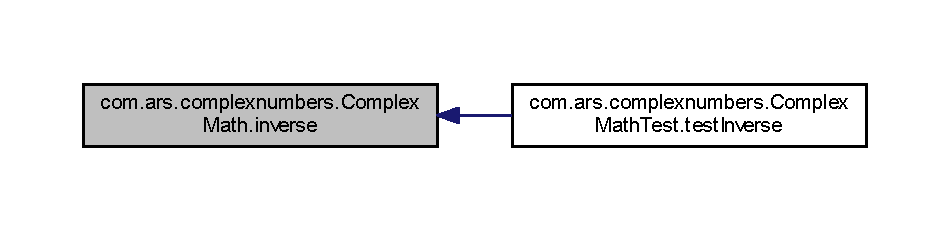
\includegraphics[width=350pt]{classcom_1_1ars_1_1complexnumbers_1_1_complex_math_a06897e69e7c59bf707851f4a502d11b8_icgraph}
\end{center}
\end{figure}
\hypertarget{classcom_1_1ars_1_1complexnumbers_1_1_complex_math_a1ffa4f4678b201779a1ac8212fc93e05}{}\label{classcom_1_1ars_1_1complexnumbers_1_1_complex_math_a1ffa4f4678b201779a1ac8212fc93e05} 
\index{com\+::ars\+::complexnumbers\+::\+Complex\+Math@{com\+::ars\+::complexnumbers\+::\+Complex\+Math}!mod@{mod}}
\index{mod@{mod}!com\+::ars\+::complexnumbers\+::\+Complex\+Math@{com\+::ars\+::complexnumbers\+::\+Complex\+Math}}
\subsubsection{\texorpdfstring{mod()}{mod()}}
{\footnotesize\ttfamily static double com.\+ars.\+complexnumbers.\+Complex\+Math.\+mod (\begin{DoxyParamCaption}\item[{\hyperlink{classcom_1_1ars_1_1complexnumbers_1_1_complex_number}{Complex\+Number}}]{z }\end{DoxyParamCaption})\hspace{0.3cm}{\ttfamily [static]}}

The modulus, magnitude or the absolute value of current complex number. 
\begin{DoxyParams}{Parameters}
{\em z} & the input complex number \\
\hline
\end{DoxyParams}
\begin{DoxyReturn}{Returns}
the modulus of number z1 
\end{DoxyReturn}
Here is the call graph for this function\+:
\nopagebreak
\begin{figure}[H]
\begin{center}
\leavevmode
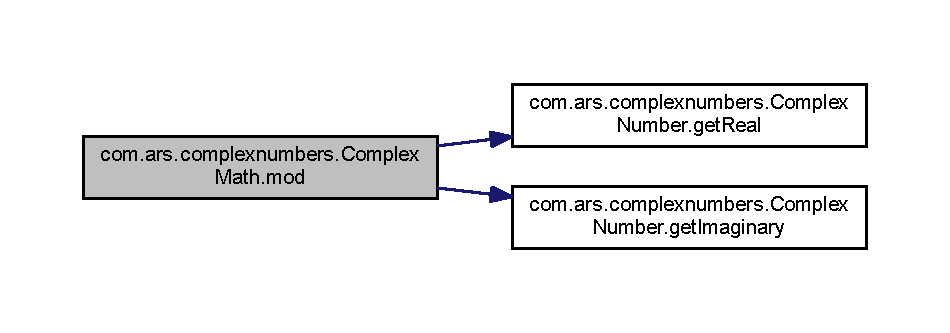
\includegraphics[width=350pt]{classcom_1_1ars_1_1complexnumbers_1_1_complex_math_a1ffa4f4678b201779a1ac8212fc93e05_cgraph}
\end{center}
\end{figure}
Here is the caller graph for this function\+:
\nopagebreak
\begin{figure}[H]
\begin{center}
\leavevmode
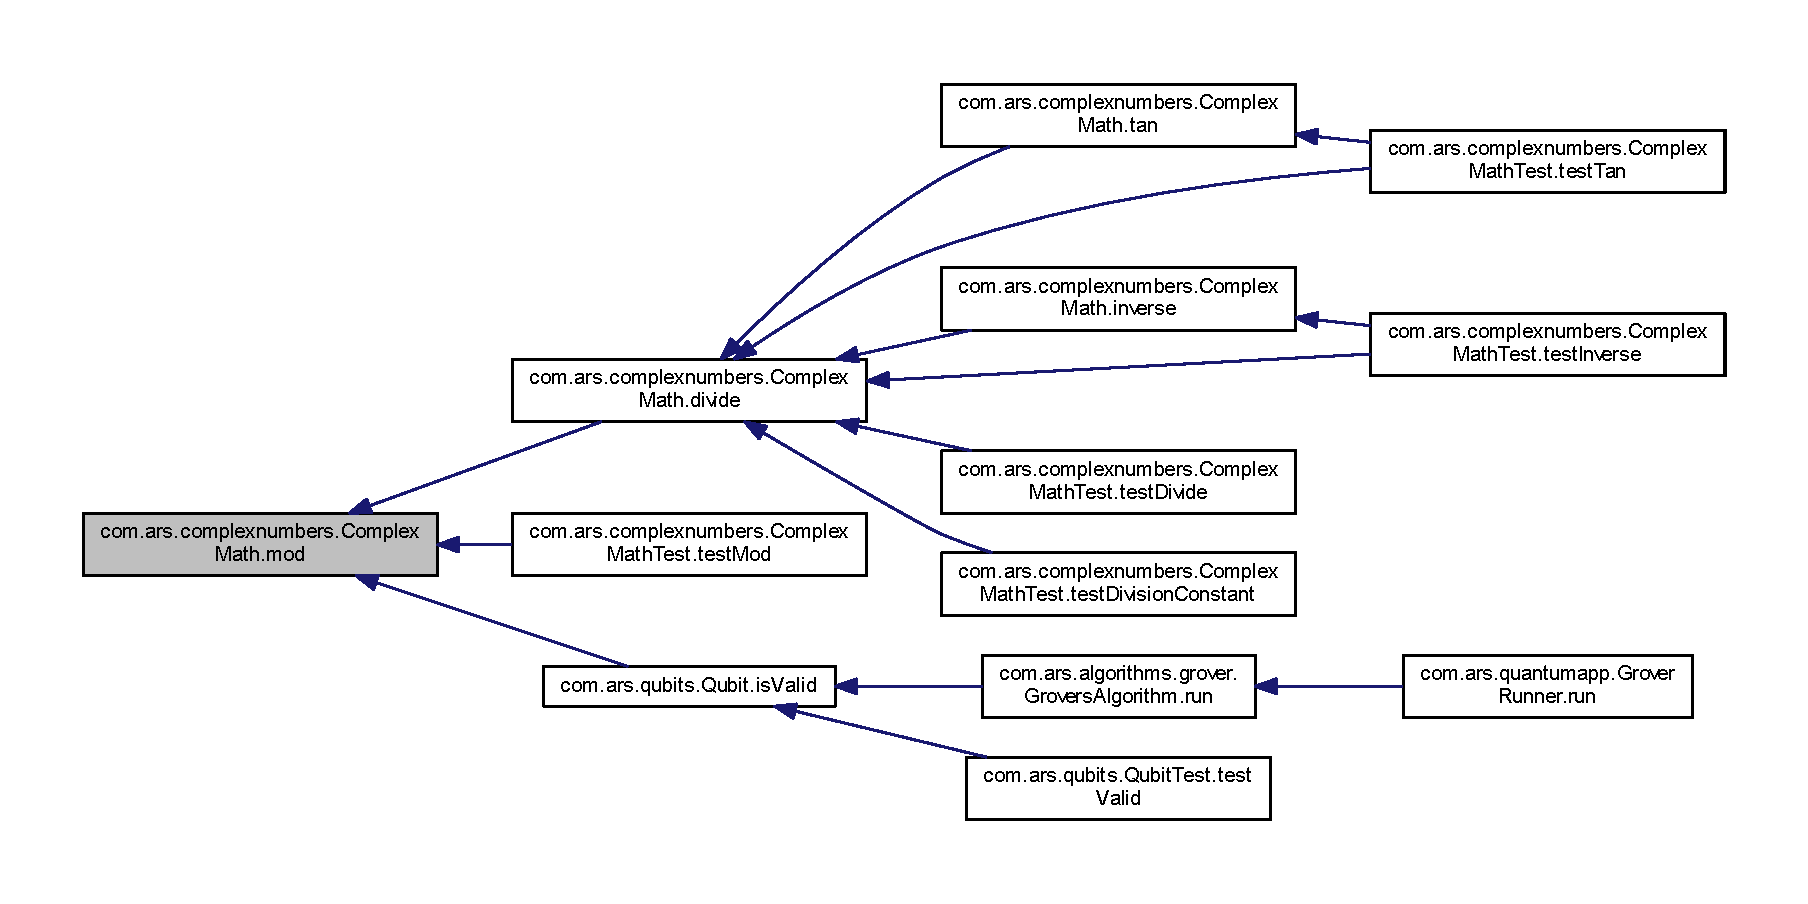
\includegraphics[width=350pt]{classcom_1_1ars_1_1complexnumbers_1_1_complex_math_a1ffa4f4678b201779a1ac8212fc93e05_icgraph}
\end{center}
\end{figure}
\hypertarget{classcom_1_1ars_1_1complexnumbers_1_1_complex_math_a0283601c9ce6efc0636468ee5e65f299}{}\label{classcom_1_1ars_1_1complexnumbers_1_1_complex_math_a0283601c9ce6efc0636468ee5e65f299} 
\index{com\+::ars\+::complexnumbers\+::\+Complex\+Math@{com\+::ars\+::complexnumbers\+::\+Complex\+Math}!multiply@{multiply}}
\index{multiply@{multiply}!com\+::ars\+::complexnumbers\+::\+Complex\+Math@{com\+::ars\+::complexnumbers\+::\+Complex\+Math}}
\subsubsection{\texorpdfstring{multiply()}{multiply()}\hspace{0.1cm}{\footnotesize\ttfamily [1/2]}}
{\footnotesize\ttfamily static \hyperlink{classcom_1_1ars_1_1complexnumbers_1_1_complex_number}{Complex\+Number} com.\+ars.\+complexnumbers.\+Complex\+Math.\+multiply (\begin{DoxyParamCaption}\item[{\hyperlink{classcom_1_1ars_1_1complexnumbers_1_1_complex_number}{Complex\+Number}}]{z1,  }\item[{\hyperlink{classcom_1_1ars_1_1complexnumbers_1_1_complex_number}{Complex\+Number}}]{z2 }\end{DoxyParamCaption})\hspace{0.3cm}{\ttfamily [static]}}

Performs the multiplication of two complex numbers. 
\begin{DoxyParams}{Parameters}
{\em z1} & first complex number \\
\hline
{\em z2} & second complex number \\
\hline
\end{DoxyParams}
\begin{DoxyReturn}{Returns}
the result of multiplication, z1 and z2, z3=z1$\ast$z2 
\end{DoxyReturn}
Here is the call graph for this function\+:
\nopagebreak
\begin{figure}[H]
\begin{center}
\leavevmode
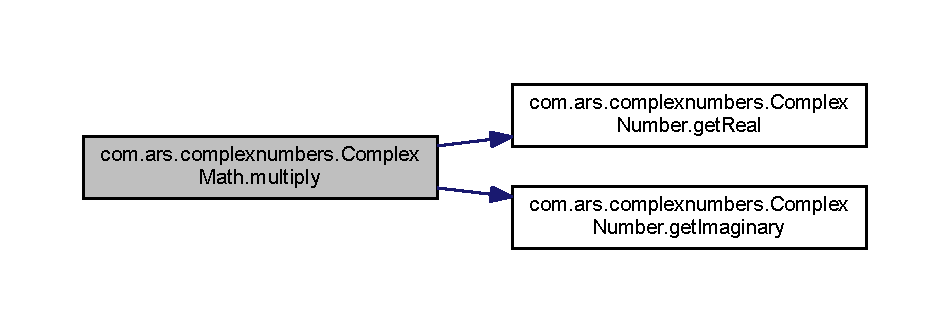
\includegraphics[width=350pt]{classcom_1_1ars_1_1complexnumbers_1_1_complex_math_a0283601c9ce6efc0636468ee5e65f299_cgraph}
\end{center}
\end{figure}
Here is the caller graph for this function\+:
\nopagebreak
\begin{figure}[H]
\begin{center}
\leavevmode
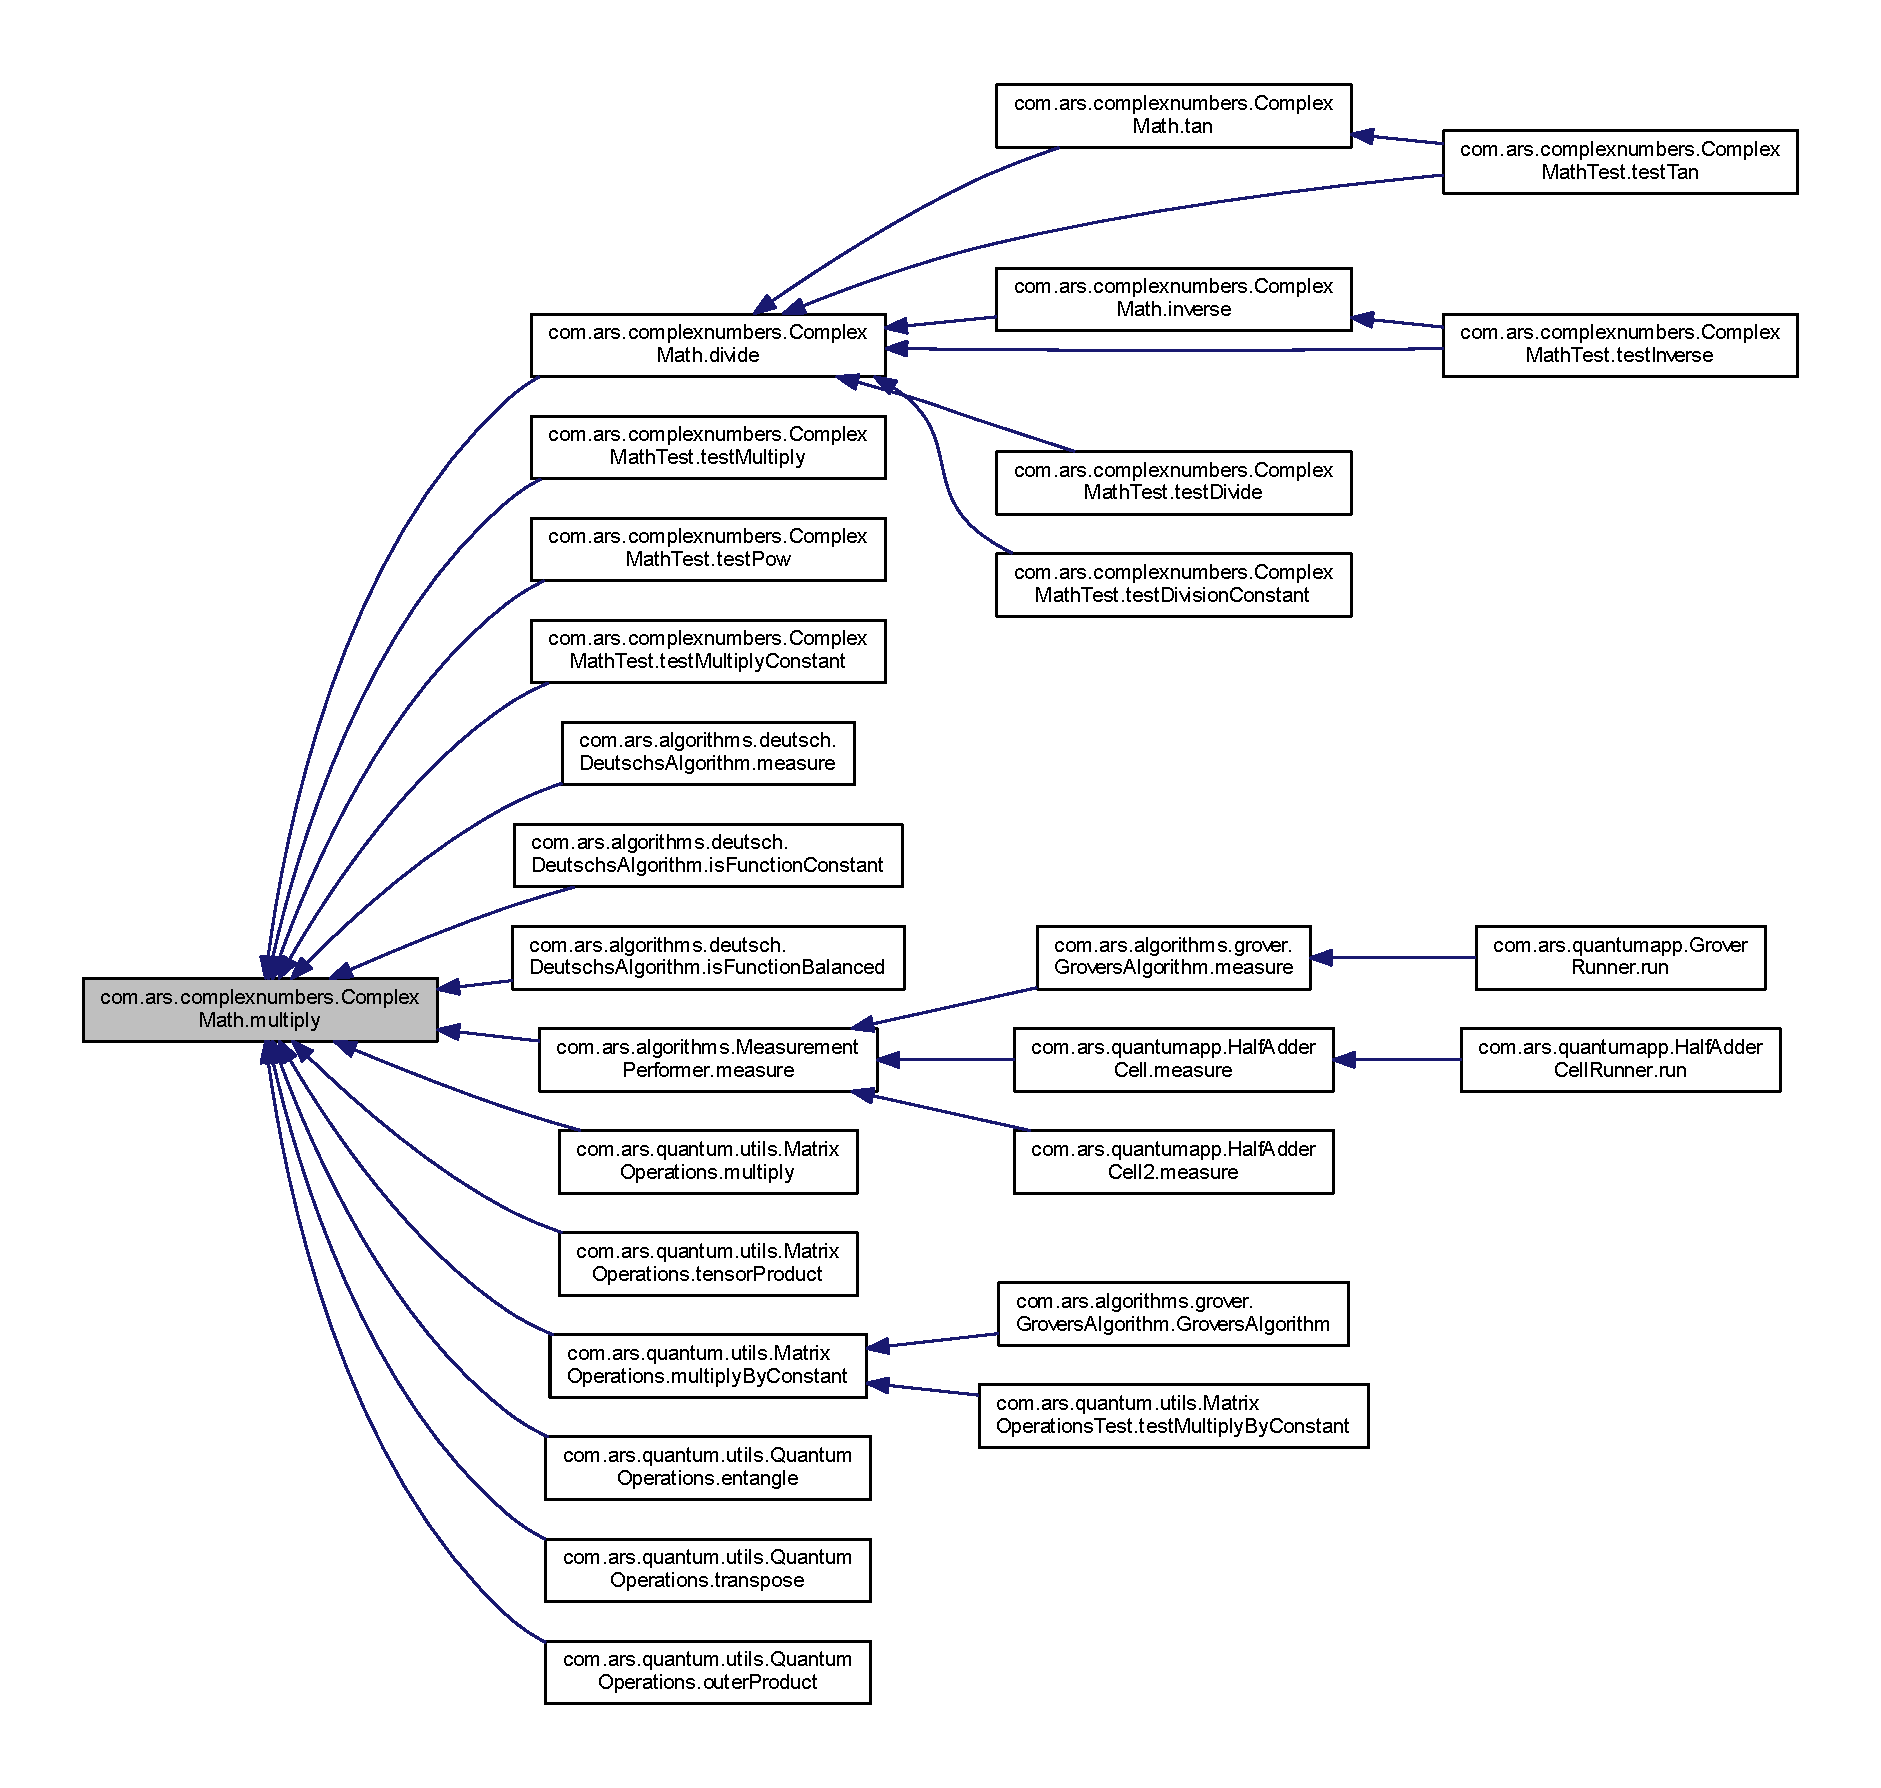
\includegraphics[width=350pt]{classcom_1_1ars_1_1complexnumbers_1_1_complex_math_a0283601c9ce6efc0636468ee5e65f299_icgraph}
\end{center}
\end{figure}
\hypertarget{classcom_1_1ars_1_1complexnumbers_1_1_complex_math_aea5e553e5a5e3e519df64cb155699198}{}\label{classcom_1_1ars_1_1complexnumbers_1_1_complex_math_aea5e553e5a5e3e519df64cb155699198} 
\index{com\+::ars\+::complexnumbers\+::\+Complex\+Math@{com\+::ars\+::complexnumbers\+::\+Complex\+Math}!multiply@{multiply}}
\index{multiply@{multiply}!com\+::ars\+::complexnumbers\+::\+Complex\+Math@{com\+::ars\+::complexnumbers\+::\+Complex\+Math}}
\subsubsection{\texorpdfstring{multiply()}{multiply()}\hspace{0.1cm}{\footnotesize\ttfamily [2/2]}}
{\footnotesize\ttfamily static \hyperlink{classcom_1_1ars_1_1complexnumbers_1_1_complex_number}{Complex\+Number} com.\+ars.\+complexnumbers.\+Complex\+Math.\+multiply (\begin{DoxyParamCaption}\item[{\hyperlink{classcom_1_1ars_1_1complexnumbers_1_1_complex_number}{Complex\+Number}}]{z,  }\item[{double}]{constant }\end{DoxyParamCaption})\hspace{0.3cm}{\ttfamily [static]}}

Performs the multiplication of a complex number with a double. 
\begin{DoxyParams}{Parameters}
{\em z} & complex number \\
\hline
{\em constant} & double number \\
\hline
\end{DoxyParams}
\begin{DoxyReturn}{Returns}
the result of multiplication. 
\end{DoxyReturn}
Here is the call graph for this function\+:
\nopagebreak
\begin{figure}[H]
\begin{center}
\leavevmode
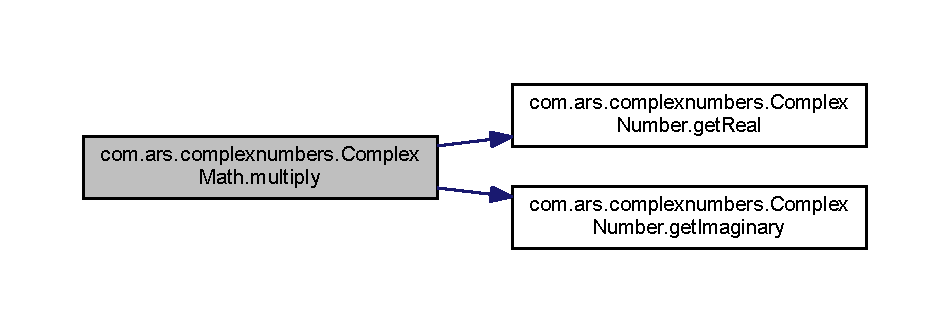
\includegraphics[width=350pt]{classcom_1_1ars_1_1complexnumbers_1_1_complex_math_aea5e553e5a5e3e519df64cb155699198_cgraph}
\end{center}
\end{figure}
\hypertarget{classcom_1_1ars_1_1complexnumbers_1_1_complex_math_a0e31bcd8237beabdee3f1480e8667d83}{}\label{classcom_1_1ars_1_1complexnumbers_1_1_complex_math_a0e31bcd8237beabdee3f1480e8667d83} 
\index{com\+::ars\+::complexnumbers\+::\+Complex\+Math@{com\+::ars\+::complexnumbers\+::\+Complex\+Math}!pow@{pow}}
\index{pow@{pow}!com\+::ars\+::complexnumbers\+::\+Complex\+Math@{com\+::ars\+::complexnumbers\+::\+Complex\+Math}}
\subsubsection{\texorpdfstring{pow()}{pow()}}
{\footnotesize\ttfamily static \hyperlink{classcom_1_1ars_1_1complexnumbers_1_1_complex_number}{Complex\+Number} com.\+ars.\+complexnumbers.\+Complex\+Math.\+pow (\begin{DoxyParamCaption}\item[{\hyperlink{classcom_1_1ars_1_1complexnumbers_1_1_complex_number}{Complex\+Number}}]{z,  }\item[{int}]{power }\end{DoxyParamCaption})\hspace{0.3cm}{\ttfamily [static]}}

Calculates the {\ttfamily \hyperlink{classcom_1_1ars_1_1complexnumbers_1_1_complex_number}{Complex\+Number}} to the passed integer power. 
\begin{DoxyParams}{Parameters}
{\em z} & the input complex number \\
\hline
{\em power} & the power \\
\hline
\end{DoxyParams}
\begin{DoxyReturn}{Returns}
return a {\ttfamily \hyperlink{classcom_1_1ars_1_1complexnumbers_1_1_complex_number}{Complex\+Number}} which is z$^\wedge$power 
\end{DoxyReturn}
Here is the call graph for this function\+:
\nopagebreak
\begin{figure}[H]
\begin{center}
\leavevmode
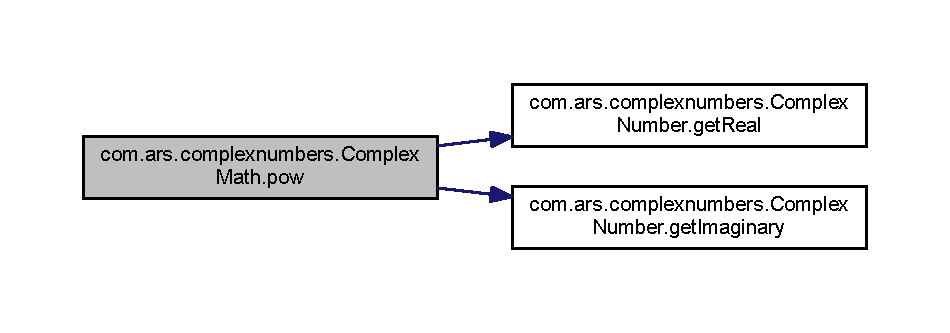
\includegraphics[width=350pt]{classcom_1_1ars_1_1complexnumbers_1_1_complex_math_a0e31bcd8237beabdee3f1480e8667d83_cgraph}
\end{center}
\end{figure}
Here is the caller graph for this function\+:
\nopagebreak
\begin{figure}[H]
\begin{center}
\leavevmode
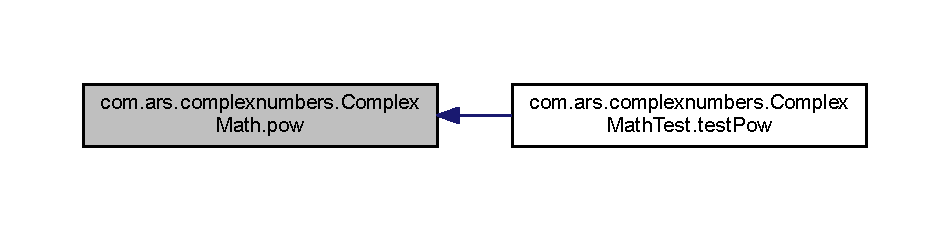
\includegraphics[width=350pt]{classcom_1_1ars_1_1complexnumbers_1_1_complex_math_a0e31bcd8237beabdee3f1480e8667d83_icgraph}
\end{center}
\end{figure}
\hypertarget{classcom_1_1ars_1_1complexnumbers_1_1_complex_math_a9c1d532e50ed32d01ccdb34d85e8765d}{}\label{classcom_1_1ars_1_1complexnumbers_1_1_complex_math_a9c1d532e50ed32d01ccdb34d85e8765d} 
\index{com\+::ars\+::complexnumbers\+::\+Complex\+Math@{com\+::ars\+::complexnumbers\+::\+Complex\+Math}!sin@{sin}}
\index{sin@{sin}!com\+::ars\+::complexnumbers\+::\+Complex\+Math@{com\+::ars\+::complexnumbers\+::\+Complex\+Math}}
\subsubsection{\texorpdfstring{sin()}{sin()}}
{\footnotesize\ttfamily static \hyperlink{classcom_1_1ars_1_1complexnumbers_1_1_complex_number}{Complex\+Number} com.\+ars.\+complexnumbers.\+Complex\+Math.\+sin (\begin{DoxyParamCaption}\item[{\hyperlink{classcom_1_1ars_1_1complexnumbers_1_1_complex_number}{Complex\+Number}}]{z }\end{DoxyParamCaption})\hspace{0.3cm}{\ttfamily [static]}}

Calculates the sine of the {\ttfamily \hyperlink{classcom_1_1ars_1_1complexnumbers_1_1_complex_number}{Complex\+Number}} 
\begin{DoxyParams}{Parameters}
{\em z} & the input complex number \\
\hline
\end{DoxyParams}
\begin{DoxyReturn}{Returns}
return a {\ttfamily \hyperlink{classcom_1_1ars_1_1complexnumbers_1_1_complex_number}{Complex\+Number}} which is sine of z 
\end{DoxyReturn}
Here is the call graph for this function\+:
\nopagebreak
\begin{figure}[H]
\begin{center}
\leavevmode
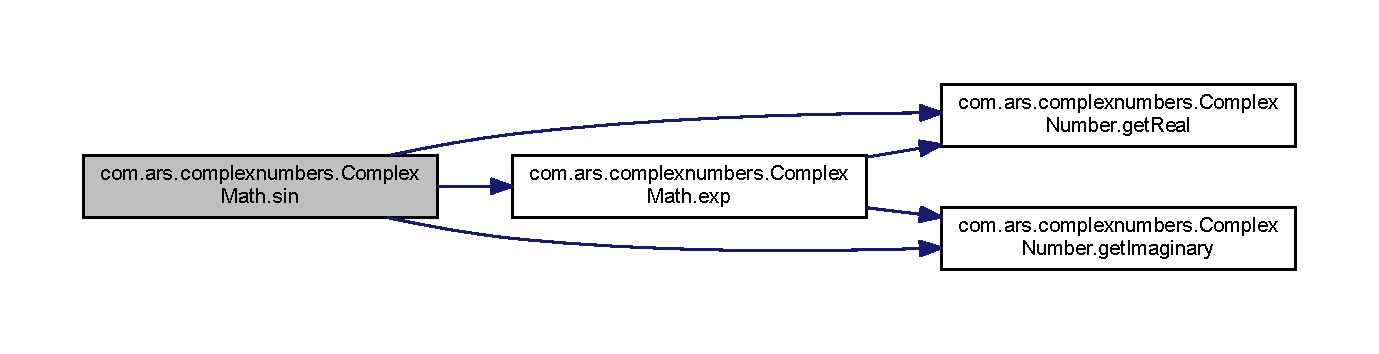
\includegraphics[width=350pt]{classcom_1_1ars_1_1complexnumbers_1_1_complex_math_a9c1d532e50ed32d01ccdb34d85e8765d_cgraph}
\end{center}
\end{figure}
Here is the caller graph for this function\+:
\nopagebreak
\begin{figure}[H]
\begin{center}
\leavevmode
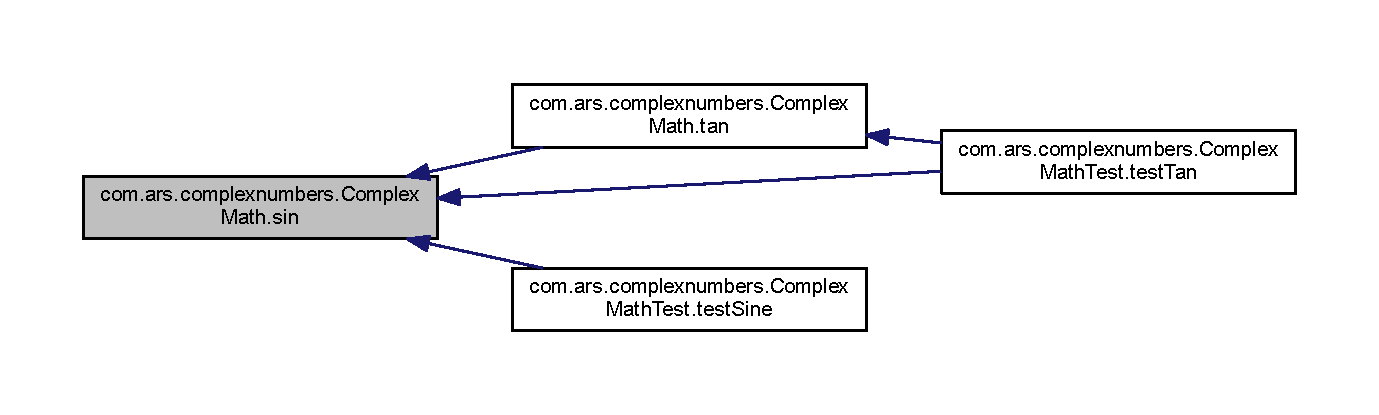
\includegraphics[width=350pt]{classcom_1_1ars_1_1complexnumbers_1_1_complex_math_a9c1d532e50ed32d01ccdb34d85e8765d_icgraph}
\end{center}
\end{figure}
\hypertarget{classcom_1_1ars_1_1complexnumbers_1_1_complex_math_ae8123eba1e8ecec75ed3d9fd05410ca2}{}\label{classcom_1_1ars_1_1complexnumbers_1_1_complex_math_ae8123eba1e8ecec75ed3d9fd05410ca2} 
\index{com\+::ars\+::complexnumbers\+::\+Complex\+Math@{com\+::ars\+::complexnumbers\+::\+Complex\+Math}!square@{square}}
\index{square@{square}!com\+::ars\+::complexnumbers\+::\+Complex\+Math@{com\+::ars\+::complexnumbers\+::\+Complex\+Math}}
\subsubsection{\texorpdfstring{square()}{square()}}
{\footnotesize\ttfamily static \hyperlink{classcom_1_1ars_1_1complexnumbers_1_1_complex_number}{Complex\+Number} com.\+ars.\+complexnumbers.\+Complex\+Math.\+square (\begin{DoxyParamCaption}\item[{\hyperlink{classcom_1_1ars_1_1complexnumbers_1_1_complex_number}{Complex\+Number}}]{z }\end{DoxyParamCaption})\hspace{0.3cm}{\ttfamily [static]}}

Calculates the square of the {\ttfamily \hyperlink{classcom_1_1ars_1_1complexnumbers_1_1_complex_number}{Complex\+Number}}. 
\begin{DoxyParams}{Parameters}
{\em z} & the input complex number \\
\hline
\end{DoxyParams}
\begin{DoxyReturn}{Returns}
the square of complex number z 
\end{DoxyReturn}
Here is the call graph for this function\+:
\nopagebreak
\begin{figure}[H]
\begin{center}
\leavevmode
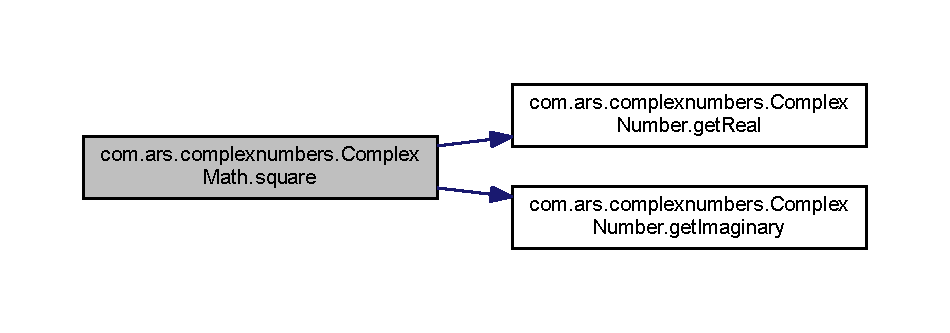
\includegraphics[width=350pt]{classcom_1_1ars_1_1complexnumbers_1_1_complex_math_ae8123eba1e8ecec75ed3d9fd05410ca2_cgraph}
\end{center}
\end{figure}
Here is the caller graph for this function\+:
\nopagebreak
\begin{figure}[H]
\begin{center}
\leavevmode
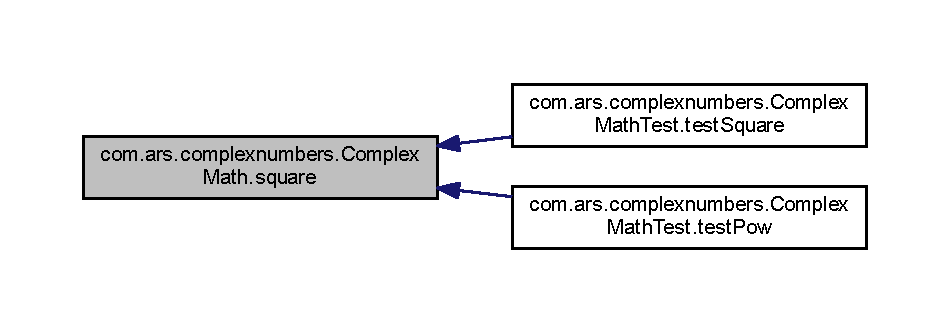
\includegraphics[width=350pt]{classcom_1_1ars_1_1complexnumbers_1_1_complex_math_ae8123eba1e8ecec75ed3d9fd05410ca2_icgraph}
\end{center}
\end{figure}
\hypertarget{classcom_1_1ars_1_1complexnumbers_1_1_complex_math_a2a8bfbcea23cec290cc91c8eeb9ab4fc}{}\label{classcom_1_1ars_1_1complexnumbers_1_1_complex_math_a2a8bfbcea23cec290cc91c8eeb9ab4fc} 
\index{com\+::ars\+::complexnumbers\+::\+Complex\+Math@{com\+::ars\+::complexnumbers\+::\+Complex\+Math}!subtract@{subtract}}
\index{subtract@{subtract}!com\+::ars\+::complexnumbers\+::\+Complex\+Math@{com\+::ars\+::complexnumbers\+::\+Complex\+Math}}
\subsubsection{\texorpdfstring{subtract()}{subtract()}\hspace{0.1cm}{\footnotesize\ttfamily [1/2]}}
{\footnotesize\ttfamily static \hyperlink{classcom_1_1ars_1_1complexnumbers_1_1_complex_number}{Complex\+Number} com.\+ars.\+complexnumbers.\+Complex\+Math.\+subtract (\begin{DoxyParamCaption}\item[{\hyperlink{classcom_1_1ars_1_1complexnumbers_1_1_complex_number}{Complex\+Number}}]{z1,  }\item[{\hyperlink{classcom_1_1ars_1_1complexnumbers_1_1_complex_number}{Complex\+Number}}]{z2 }\end{DoxyParamCaption})\hspace{0.3cm}{\ttfamily [static]}}

Performs the subtraction of two complex numbers. 
\begin{DoxyParams}{Parameters}
{\em z1} & first complex number \\
\hline
{\em z2} & second complex number \\
\hline
\end{DoxyParams}
\begin{DoxyReturn}{Returns}
the result of subtraction, z1 and z2, z3=z1-\/z2 
\end{DoxyReturn}
Here is the call graph for this function\+:
\nopagebreak
\begin{figure}[H]
\begin{center}
\leavevmode
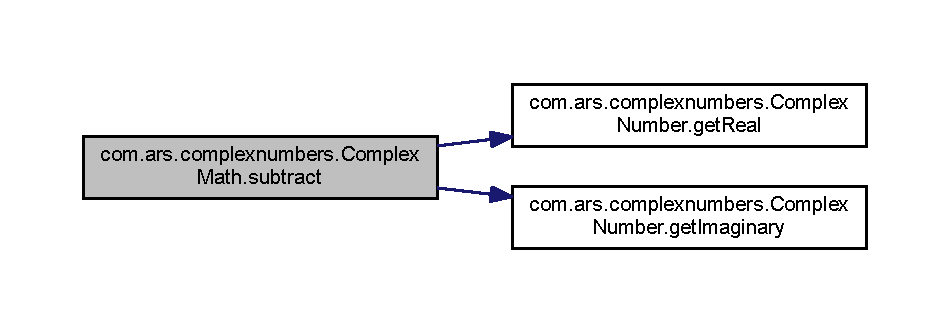
\includegraphics[width=350pt]{classcom_1_1ars_1_1complexnumbers_1_1_complex_math_a2a8bfbcea23cec290cc91c8eeb9ab4fc_cgraph}
\end{center}
\end{figure}
Here is the caller graph for this function\+:
\nopagebreak
\begin{figure}[H]
\begin{center}
\leavevmode
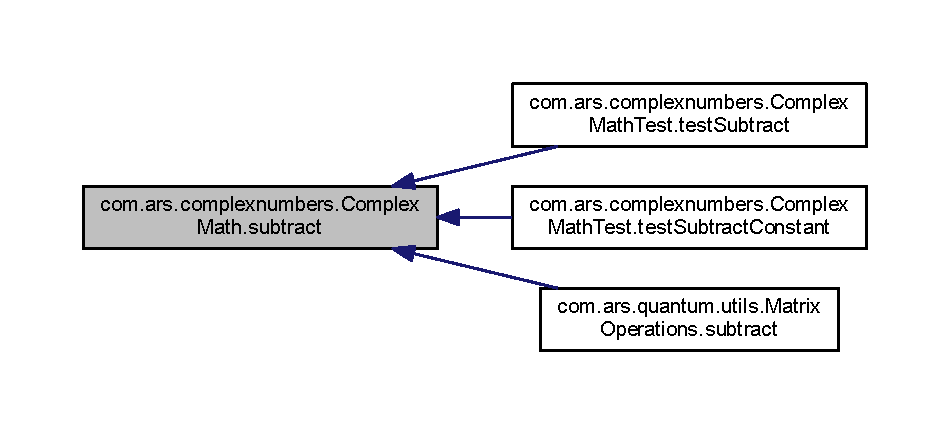
\includegraphics[width=350pt]{classcom_1_1ars_1_1complexnumbers_1_1_complex_math_a2a8bfbcea23cec290cc91c8eeb9ab4fc_icgraph}
\end{center}
\end{figure}
\hypertarget{classcom_1_1ars_1_1complexnumbers_1_1_complex_math_a8ec234a476d41f2f32113eb13a0f7630}{}\label{classcom_1_1ars_1_1complexnumbers_1_1_complex_math_a8ec234a476d41f2f32113eb13a0f7630} 
\index{com\+::ars\+::complexnumbers\+::\+Complex\+Math@{com\+::ars\+::complexnumbers\+::\+Complex\+Math}!subtract@{subtract}}
\index{subtract@{subtract}!com\+::ars\+::complexnumbers\+::\+Complex\+Math@{com\+::ars\+::complexnumbers\+::\+Complex\+Math}}
\subsubsection{\texorpdfstring{subtract()}{subtract()}\hspace{0.1cm}{\footnotesize\ttfamily [2/2]}}
{\footnotesize\ttfamily static \hyperlink{classcom_1_1ars_1_1complexnumbers_1_1_complex_number}{Complex\+Number} com.\+ars.\+complexnumbers.\+Complex\+Math.\+subtract (\begin{DoxyParamCaption}\item[{\hyperlink{classcom_1_1ars_1_1complexnumbers_1_1_complex_number}{Complex\+Number}}]{z,  }\item[{double}]{constant }\end{DoxyParamCaption})\hspace{0.3cm}{\ttfamily [static]}}

Performs the subtraction of a complex number with a double. 
\begin{DoxyParams}{Parameters}
{\em z} & complex number \\
\hline
{\em constant} & double number \\
\hline
\end{DoxyParams}
\begin{DoxyReturn}{Returns}
the result of subtraction. 
\end{DoxyReturn}
Here is the call graph for this function\+:
\nopagebreak
\begin{figure}[H]
\begin{center}
\leavevmode
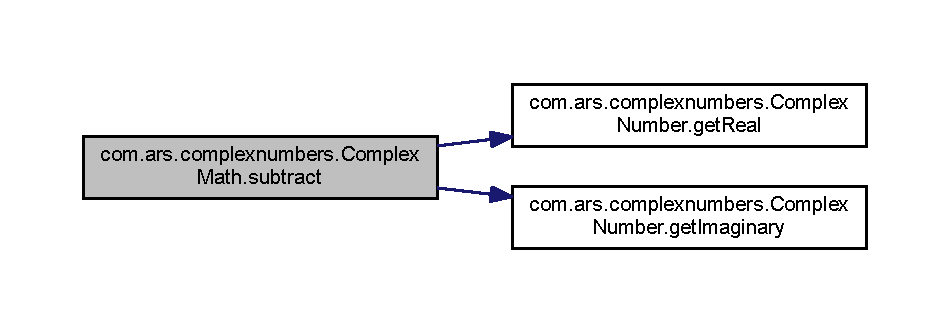
\includegraphics[width=350pt]{classcom_1_1ars_1_1complexnumbers_1_1_complex_math_a8ec234a476d41f2f32113eb13a0f7630_cgraph}
\end{center}
\end{figure}
\hypertarget{classcom_1_1ars_1_1complexnumbers_1_1_complex_math_af260af539eaec79d57b7e5363bda686e}{}\label{classcom_1_1ars_1_1complexnumbers_1_1_complex_math_af260af539eaec79d57b7e5363bda686e} 
\index{com\+::ars\+::complexnumbers\+::\+Complex\+Math@{com\+::ars\+::complexnumbers\+::\+Complex\+Math}!tan@{tan}}
\index{tan@{tan}!com\+::ars\+::complexnumbers\+::\+Complex\+Math@{com\+::ars\+::complexnumbers\+::\+Complex\+Math}}
\subsubsection{\texorpdfstring{tan()}{tan()}}
{\footnotesize\ttfamily static \hyperlink{classcom_1_1ars_1_1complexnumbers_1_1_complex_number}{Complex\+Number} com.\+ars.\+complexnumbers.\+Complex\+Math.\+tan (\begin{DoxyParamCaption}\item[{\hyperlink{classcom_1_1ars_1_1complexnumbers_1_1_complex_number}{Complex\+Number}}]{z }\end{DoxyParamCaption})\hspace{0.3cm}{\ttfamily [static]}}

Calculates the tangent of the {\ttfamily \hyperlink{classcom_1_1ars_1_1complexnumbers_1_1_complex_number}{Complex\+Number}} 
\begin{DoxyParams}{Parameters}
{\em z} & the input complex number \\
\hline
\end{DoxyParams}
\begin{DoxyReturn}{Returns}
return a {\ttfamily \hyperlink{classcom_1_1ars_1_1complexnumbers_1_1_complex_number}{Complex\+Number}} which is tangent of z 
\end{DoxyReturn}
Here is the call graph for this function\+:
\nopagebreak
\begin{figure}[H]
\begin{center}
\leavevmode
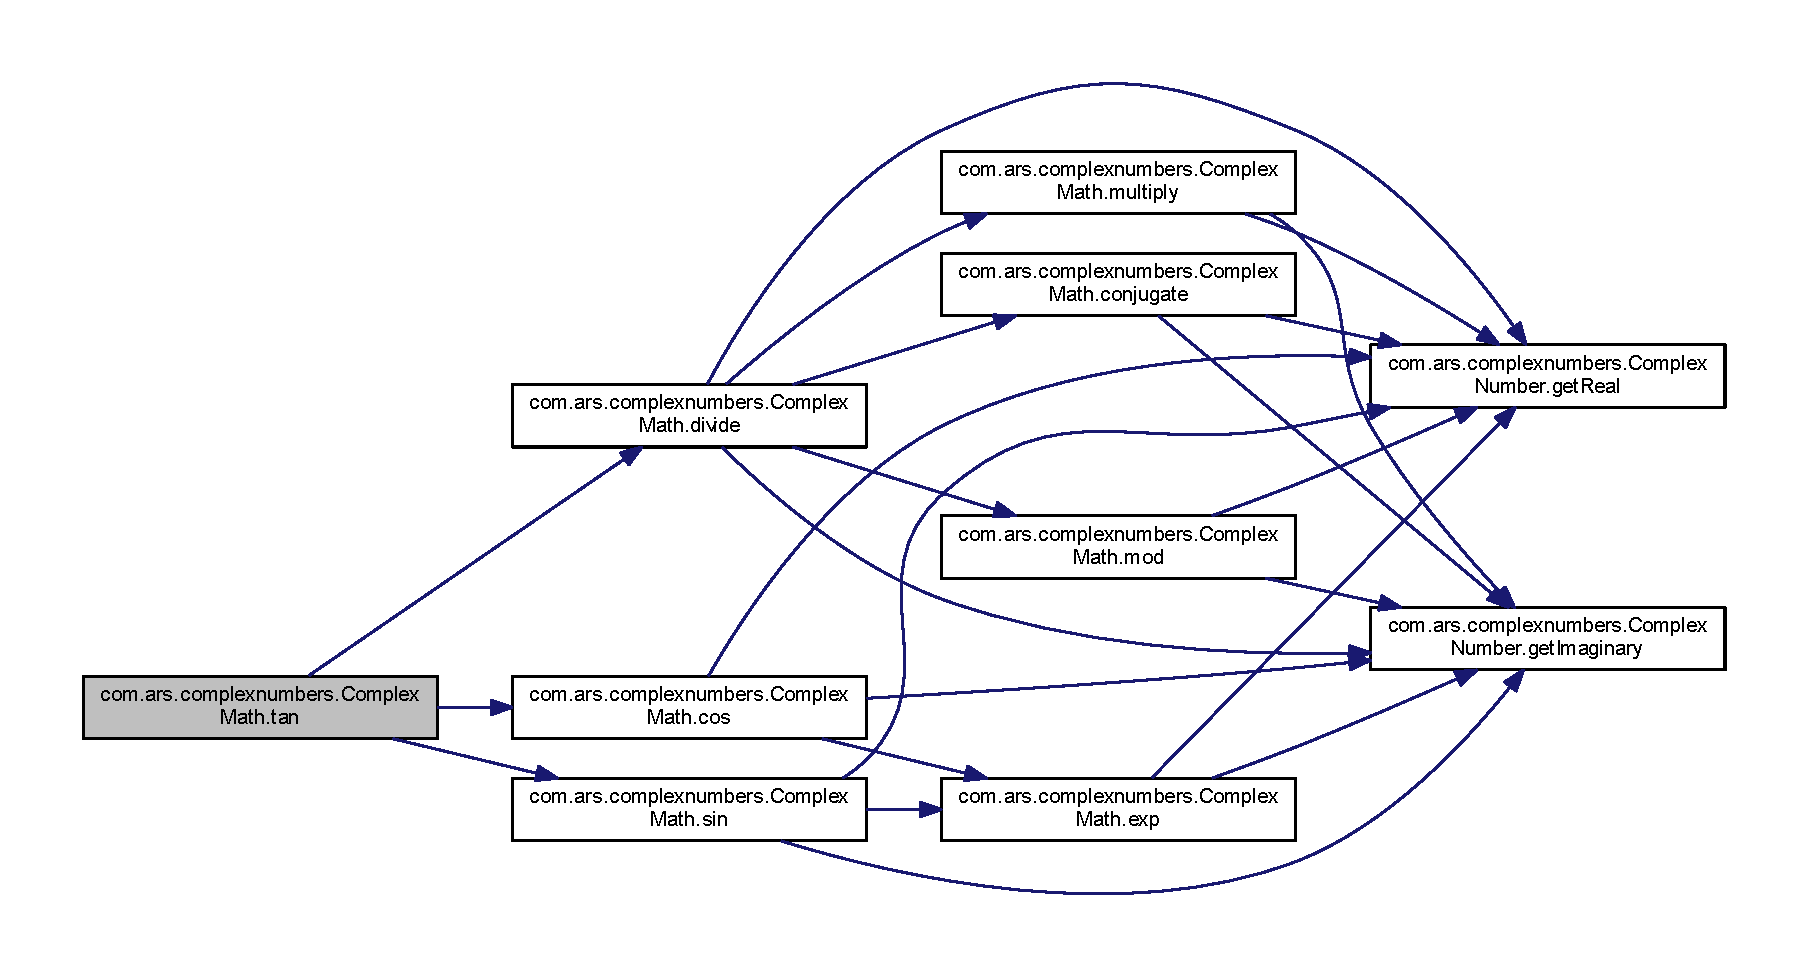
\includegraphics[width=350pt]{classcom_1_1ars_1_1complexnumbers_1_1_complex_math_af260af539eaec79d57b7e5363bda686e_cgraph}
\end{center}
\end{figure}
Here is the caller graph for this function\+:
\nopagebreak
\begin{figure}[H]
\begin{center}
\leavevmode
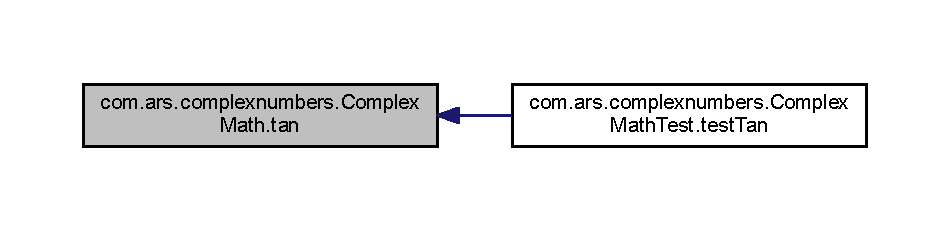
\includegraphics[width=350pt]{classcom_1_1ars_1_1complexnumbers_1_1_complex_math_af260af539eaec79d57b7e5363bda686e_icgraph}
\end{center}
\end{figure}


The documentation for this class was generated from the following file\+:\begin{DoxyCompactItemize}
\item 
C\+:/\+Users/\+Dacian/\+Desktop/\+Quantum/\+Quantum/quantum\+\_\+computing-\/master/complexnumbers/src/main/java/com/ars/complexnumbers/\hyperlink{_complex_math_8java}{Complex\+Math.\+java}\end{DoxyCompactItemize}

\hypertarget{classcom_1_1ars_1_1complexnumbers_1_1_complex_math_test}{}\section{com.\+ars.\+complexnumbers.\+Complex\+Math\+Test Class Reference}
\label{classcom_1_1ars_1_1complexnumbers_1_1_complex_math_test}\index{com.\+ars.\+complexnumbers.\+Complex\+Math\+Test@{com.\+ars.\+complexnumbers.\+Complex\+Math\+Test}}
\subsection*{Public Member Functions}
\begin{DoxyCompactItemize}
\item 
void \hyperlink{classcom_1_1ars_1_1complexnumbers_1_1_complex_math_test_a038ac671e0502ed2448f4649da993131}{set\+Up} ()  throws Exception 
\item 
void \hyperlink{classcom_1_1ars_1_1complexnumbers_1_1_complex_math_test_aa0a4283d8c92cfd428208a61fb0b2753}{tear\+Down} ()  throws Exception 
\item 
void \hyperlink{classcom_1_1ars_1_1complexnumbers_1_1_complex_math_test_a29817014ba09b1d2f985882ddfcbfae2}{test\+Conjugate} ()
\item 
void \hyperlink{classcom_1_1ars_1_1complexnumbers_1_1_complex_math_test_af1b3b844bab2323d1bd4bb07712f7652}{test\+Mod} ()
\item 
void \hyperlink{classcom_1_1ars_1_1complexnumbers_1_1_complex_math_test_a820df886e3c20f3cbe36ff6905e1d67e}{test\+Add} ()
\item 
void \hyperlink{classcom_1_1ars_1_1complexnumbers_1_1_complex_math_test_a79e2b206d48588b1e7db17a681a405eb}{test\+Subtract} ()
\item 
void \hyperlink{classcom_1_1ars_1_1complexnumbers_1_1_complex_math_test_a195e4c9c2b94ada809ff5ca462a9dc06}{test\+Multiply} ()
\item 
void \hyperlink{classcom_1_1ars_1_1complexnumbers_1_1_complex_math_test_a8ddaa1e32717e2b18f6c64010c688b6d}{test\+Divide} ()
\item 
void \hyperlink{classcom_1_1ars_1_1complexnumbers_1_1_complex_math_test_a43dc686fe2b96e097f3ee8095fef12c1}{test\+Square} ()
\item 
void \hyperlink{classcom_1_1ars_1_1complexnumbers_1_1_complex_math_test_ab429903cc819ea2c83369e07ba2f49e9}{test\+Sine} ()
\item 
void \hyperlink{classcom_1_1ars_1_1complexnumbers_1_1_complex_math_test_a453b6e66b0570b74892caa9ec83c47cb}{test\+Cosine} ()
\item 
void \hyperlink{classcom_1_1ars_1_1complexnumbers_1_1_complex_math_test_abcec8968bf43093a912ba2c24f4718a9}{test\+Tan} ()
\item 
void \hyperlink{classcom_1_1ars_1_1complexnumbers_1_1_complex_math_test_abd1ea731d0875c3351306079e4694c24}{test\+Exp} ()
\item 
void \hyperlink{classcom_1_1ars_1_1complexnumbers_1_1_complex_math_test_a70af211131478c43b06210fe524d3bd7}{test\+Pow} ()
\item 
void \hyperlink{classcom_1_1ars_1_1complexnumbers_1_1_complex_math_test_a2102465aa80b8303b2de77a3e87ffea9}{test\+Get\+Arg} ()
\item 
void \hyperlink{classcom_1_1ars_1_1complexnumbers_1_1_complex_math_test_a2c47b64252c4ecbe00d38fe89e66a9bb}{test\+Inverse} ()
\item 
void \hyperlink{classcom_1_1ars_1_1complexnumbers_1_1_complex_math_test_a118231be2a26c23d165d3b40093352ac}{test\+Multiply\+Constant} ()
\item 
void \hyperlink{classcom_1_1ars_1_1complexnumbers_1_1_complex_math_test_a7250df204110c40becd58a0886ec8e7c}{test\+Division\+Constant} ()
\item 
void \hyperlink{classcom_1_1ars_1_1complexnumbers_1_1_complex_math_test_a0dba8a864962376e684cfcbc1baa80f4}{test\+Add\+Constant} ()
\item 
void \hyperlink{classcom_1_1ars_1_1complexnumbers_1_1_complex_math_test_a535b2562407e9de2c6aea700d5e1a0f8}{test\+Subtract\+Constant} ()
\end{DoxyCompactItemize}


\subsection{Member Function Documentation}
\hypertarget{classcom_1_1ars_1_1complexnumbers_1_1_complex_math_test_a038ac671e0502ed2448f4649da993131}{}\label{classcom_1_1ars_1_1complexnumbers_1_1_complex_math_test_a038ac671e0502ed2448f4649da993131} 
\index{com\+::ars\+::complexnumbers\+::\+Complex\+Math\+Test@{com\+::ars\+::complexnumbers\+::\+Complex\+Math\+Test}!set\+Up@{set\+Up}}
\index{set\+Up@{set\+Up}!com\+::ars\+::complexnumbers\+::\+Complex\+Math\+Test@{com\+::ars\+::complexnumbers\+::\+Complex\+Math\+Test}}
\subsubsection{\texorpdfstring{set\+Up()}{setUp()}}
{\footnotesize\ttfamily void com.\+ars.\+complexnumbers.\+Complex\+Math\+Test.\+set\+Up (\begin{DoxyParamCaption}{ }\end{DoxyParamCaption}) throws Exception}

\hypertarget{classcom_1_1ars_1_1complexnumbers_1_1_complex_math_test_aa0a4283d8c92cfd428208a61fb0b2753}{}\label{classcom_1_1ars_1_1complexnumbers_1_1_complex_math_test_aa0a4283d8c92cfd428208a61fb0b2753} 
\index{com\+::ars\+::complexnumbers\+::\+Complex\+Math\+Test@{com\+::ars\+::complexnumbers\+::\+Complex\+Math\+Test}!tear\+Down@{tear\+Down}}
\index{tear\+Down@{tear\+Down}!com\+::ars\+::complexnumbers\+::\+Complex\+Math\+Test@{com\+::ars\+::complexnumbers\+::\+Complex\+Math\+Test}}
\subsubsection{\texorpdfstring{tear\+Down()}{tearDown()}}
{\footnotesize\ttfamily void com.\+ars.\+complexnumbers.\+Complex\+Math\+Test.\+tear\+Down (\begin{DoxyParamCaption}{ }\end{DoxyParamCaption}) throws Exception}

\hypertarget{classcom_1_1ars_1_1complexnumbers_1_1_complex_math_test_a820df886e3c20f3cbe36ff6905e1d67e}{}\label{classcom_1_1ars_1_1complexnumbers_1_1_complex_math_test_a820df886e3c20f3cbe36ff6905e1d67e} 
\index{com\+::ars\+::complexnumbers\+::\+Complex\+Math\+Test@{com\+::ars\+::complexnumbers\+::\+Complex\+Math\+Test}!test\+Add@{test\+Add}}
\index{test\+Add@{test\+Add}!com\+::ars\+::complexnumbers\+::\+Complex\+Math\+Test@{com\+::ars\+::complexnumbers\+::\+Complex\+Math\+Test}}
\subsubsection{\texorpdfstring{test\+Add()}{testAdd()}}
{\footnotesize\ttfamily void com.\+ars.\+complexnumbers.\+Complex\+Math\+Test.\+test\+Add (\begin{DoxyParamCaption}{ }\end{DoxyParamCaption})}

Here is the call graph for this function\+:\nopagebreak
\begin{figure}[H]
\begin{center}
\leavevmode
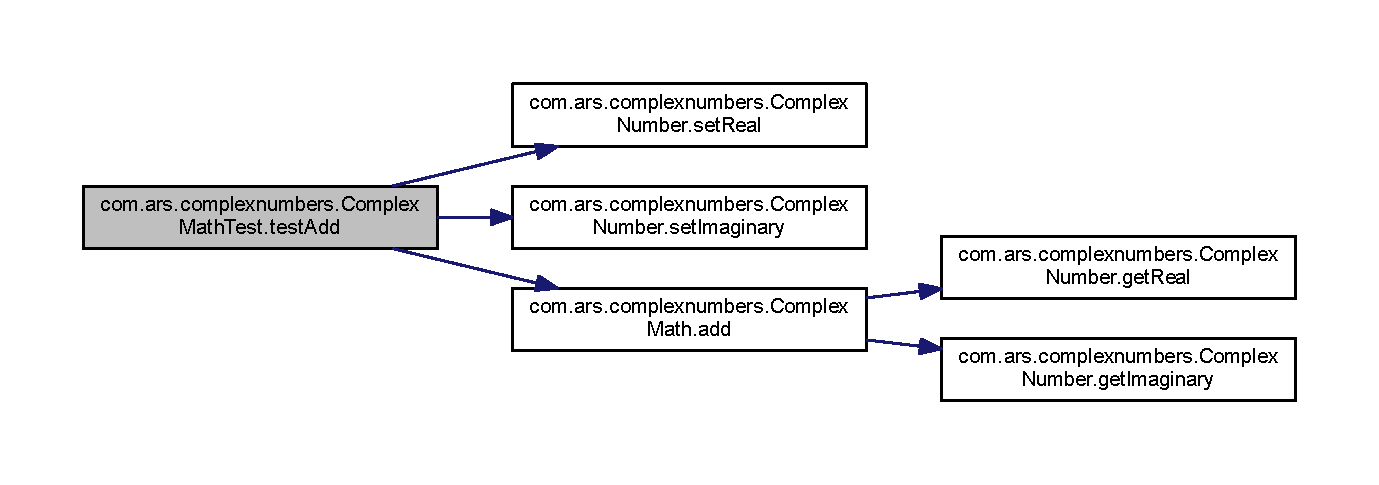
\includegraphics[width=350pt]{classcom_1_1ars_1_1complexnumbers_1_1_complex_math_test_a820df886e3c20f3cbe36ff6905e1d67e_cgraph}
\end{center}
\end{figure}
\hypertarget{classcom_1_1ars_1_1complexnumbers_1_1_complex_math_test_a0dba8a864962376e684cfcbc1baa80f4}{}\label{classcom_1_1ars_1_1complexnumbers_1_1_complex_math_test_a0dba8a864962376e684cfcbc1baa80f4} 
\index{com\+::ars\+::complexnumbers\+::\+Complex\+Math\+Test@{com\+::ars\+::complexnumbers\+::\+Complex\+Math\+Test}!test\+Add\+Constant@{test\+Add\+Constant}}
\index{test\+Add\+Constant@{test\+Add\+Constant}!com\+::ars\+::complexnumbers\+::\+Complex\+Math\+Test@{com\+::ars\+::complexnumbers\+::\+Complex\+Math\+Test}}
\subsubsection{\texorpdfstring{test\+Add\+Constant()}{testAddConstant()}}
{\footnotesize\ttfamily void com.\+ars.\+complexnumbers.\+Complex\+Math\+Test.\+test\+Add\+Constant (\begin{DoxyParamCaption}{ }\end{DoxyParamCaption})}

Here is the call graph for this function\+:\nopagebreak
\begin{figure}[H]
\begin{center}
\leavevmode
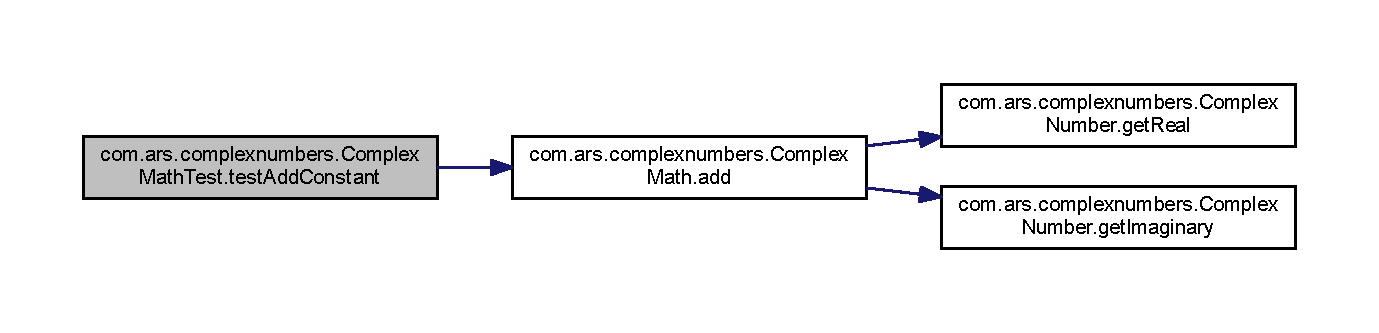
\includegraphics[width=350pt]{classcom_1_1ars_1_1complexnumbers_1_1_complex_math_test_a0dba8a864962376e684cfcbc1baa80f4_cgraph}
\end{center}
\end{figure}
\hypertarget{classcom_1_1ars_1_1complexnumbers_1_1_complex_math_test_a29817014ba09b1d2f985882ddfcbfae2}{}\label{classcom_1_1ars_1_1complexnumbers_1_1_complex_math_test_a29817014ba09b1d2f985882ddfcbfae2} 
\index{com\+::ars\+::complexnumbers\+::\+Complex\+Math\+Test@{com\+::ars\+::complexnumbers\+::\+Complex\+Math\+Test}!test\+Conjugate@{test\+Conjugate}}
\index{test\+Conjugate@{test\+Conjugate}!com\+::ars\+::complexnumbers\+::\+Complex\+Math\+Test@{com\+::ars\+::complexnumbers\+::\+Complex\+Math\+Test}}
\subsubsection{\texorpdfstring{test\+Conjugate()}{testConjugate()}}
{\footnotesize\ttfamily void com.\+ars.\+complexnumbers.\+Complex\+Math\+Test.\+test\+Conjugate (\begin{DoxyParamCaption}{ }\end{DoxyParamCaption})}

Here is the call graph for this function\+:\nopagebreak
\begin{figure}[H]
\begin{center}
\leavevmode
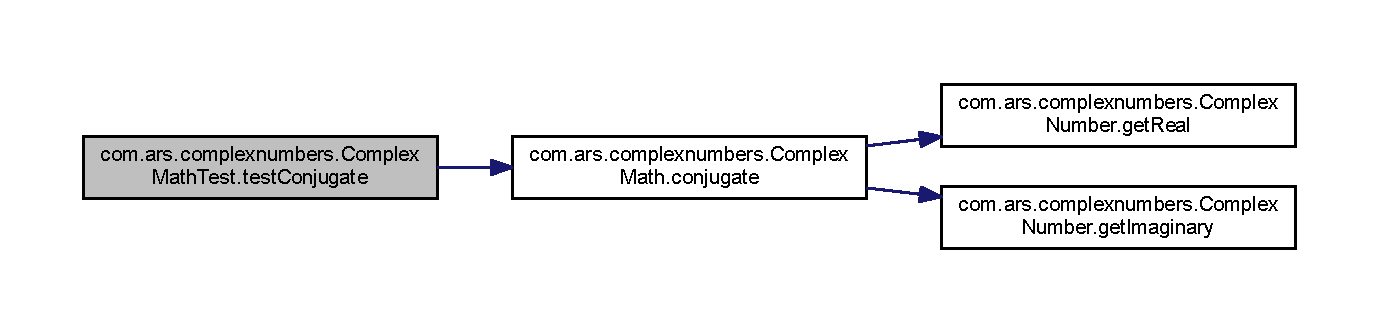
\includegraphics[width=350pt]{classcom_1_1ars_1_1complexnumbers_1_1_complex_math_test_a29817014ba09b1d2f985882ddfcbfae2_cgraph}
\end{center}
\end{figure}
\hypertarget{classcom_1_1ars_1_1complexnumbers_1_1_complex_math_test_a453b6e66b0570b74892caa9ec83c47cb}{}\label{classcom_1_1ars_1_1complexnumbers_1_1_complex_math_test_a453b6e66b0570b74892caa9ec83c47cb} 
\index{com\+::ars\+::complexnumbers\+::\+Complex\+Math\+Test@{com\+::ars\+::complexnumbers\+::\+Complex\+Math\+Test}!test\+Cosine@{test\+Cosine}}
\index{test\+Cosine@{test\+Cosine}!com\+::ars\+::complexnumbers\+::\+Complex\+Math\+Test@{com\+::ars\+::complexnumbers\+::\+Complex\+Math\+Test}}
\subsubsection{\texorpdfstring{test\+Cosine()}{testCosine()}}
{\footnotesize\ttfamily void com.\+ars.\+complexnumbers.\+Complex\+Math\+Test.\+test\+Cosine (\begin{DoxyParamCaption}{ }\end{DoxyParamCaption})}

Here is the call graph for this function\+:\nopagebreak
\begin{figure}[H]
\begin{center}
\leavevmode
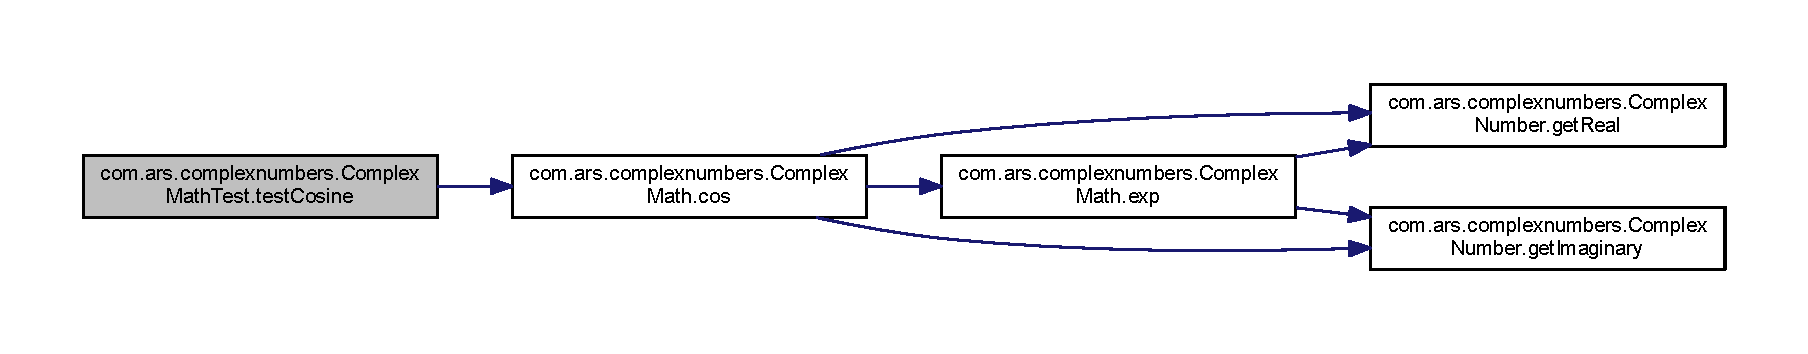
\includegraphics[width=350pt]{classcom_1_1ars_1_1complexnumbers_1_1_complex_math_test_a453b6e66b0570b74892caa9ec83c47cb_cgraph}
\end{center}
\end{figure}
\hypertarget{classcom_1_1ars_1_1complexnumbers_1_1_complex_math_test_a8ddaa1e32717e2b18f6c64010c688b6d}{}\label{classcom_1_1ars_1_1complexnumbers_1_1_complex_math_test_a8ddaa1e32717e2b18f6c64010c688b6d} 
\index{com\+::ars\+::complexnumbers\+::\+Complex\+Math\+Test@{com\+::ars\+::complexnumbers\+::\+Complex\+Math\+Test}!test\+Divide@{test\+Divide}}
\index{test\+Divide@{test\+Divide}!com\+::ars\+::complexnumbers\+::\+Complex\+Math\+Test@{com\+::ars\+::complexnumbers\+::\+Complex\+Math\+Test}}
\subsubsection{\texorpdfstring{test\+Divide()}{testDivide()}}
{\footnotesize\ttfamily void com.\+ars.\+complexnumbers.\+Complex\+Math\+Test.\+test\+Divide (\begin{DoxyParamCaption}{ }\end{DoxyParamCaption})}

Here is the call graph for this function\+:\nopagebreak
\begin{figure}[H]
\begin{center}
\leavevmode
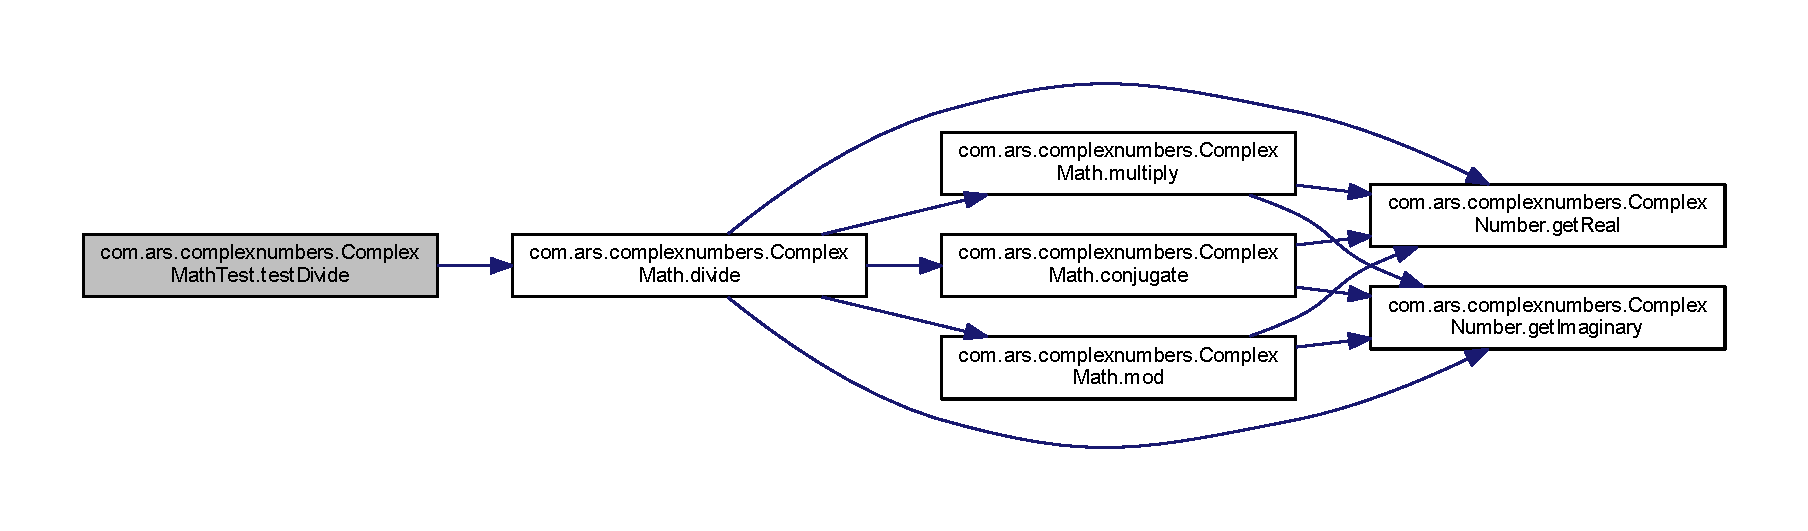
\includegraphics[width=350pt]{classcom_1_1ars_1_1complexnumbers_1_1_complex_math_test_a8ddaa1e32717e2b18f6c64010c688b6d_cgraph}
\end{center}
\end{figure}
\hypertarget{classcom_1_1ars_1_1complexnumbers_1_1_complex_math_test_a7250df204110c40becd58a0886ec8e7c}{}\label{classcom_1_1ars_1_1complexnumbers_1_1_complex_math_test_a7250df204110c40becd58a0886ec8e7c} 
\index{com\+::ars\+::complexnumbers\+::\+Complex\+Math\+Test@{com\+::ars\+::complexnumbers\+::\+Complex\+Math\+Test}!test\+Division\+Constant@{test\+Division\+Constant}}
\index{test\+Division\+Constant@{test\+Division\+Constant}!com\+::ars\+::complexnumbers\+::\+Complex\+Math\+Test@{com\+::ars\+::complexnumbers\+::\+Complex\+Math\+Test}}
\subsubsection{\texorpdfstring{test\+Division\+Constant()}{testDivisionConstant()}}
{\footnotesize\ttfamily void com.\+ars.\+complexnumbers.\+Complex\+Math\+Test.\+test\+Division\+Constant (\begin{DoxyParamCaption}{ }\end{DoxyParamCaption})}

Here is the call graph for this function\+:\nopagebreak
\begin{figure}[H]
\begin{center}
\leavevmode
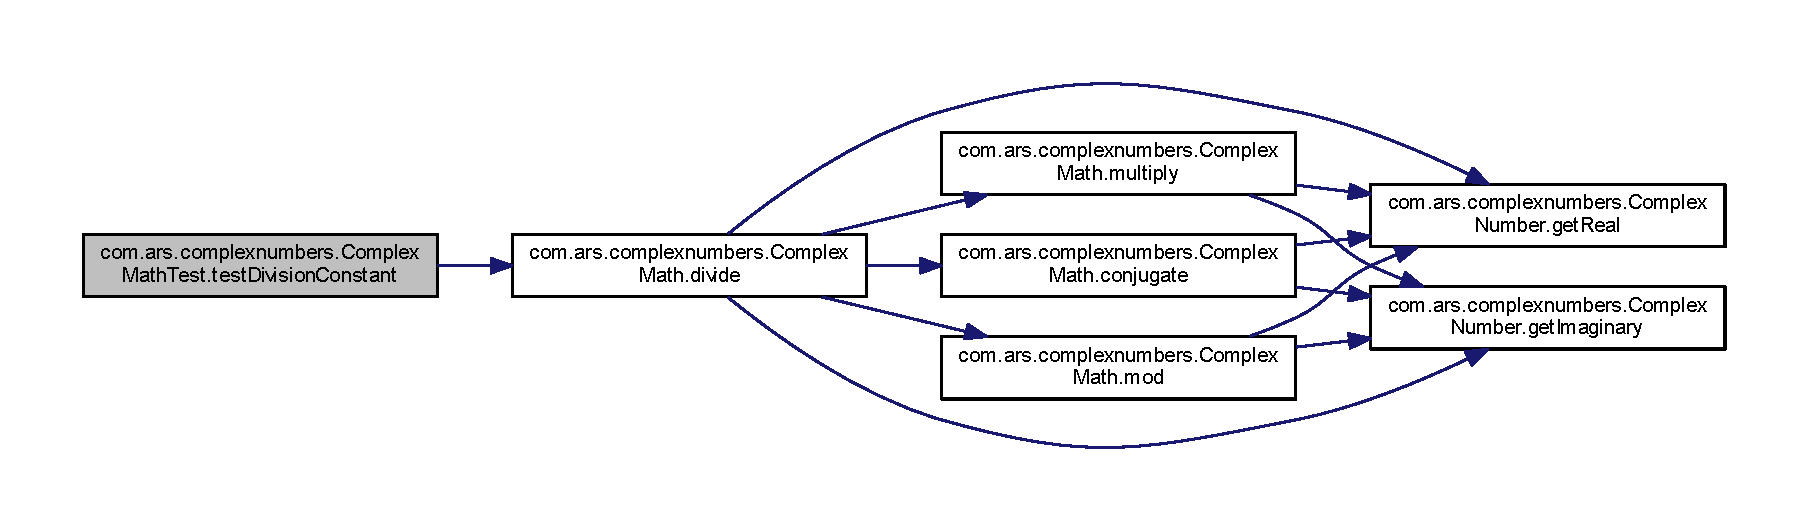
\includegraphics[width=350pt]{classcom_1_1ars_1_1complexnumbers_1_1_complex_math_test_a7250df204110c40becd58a0886ec8e7c_cgraph}
\end{center}
\end{figure}
\hypertarget{classcom_1_1ars_1_1complexnumbers_1_1_complex_math_test_abd1ea731d0875c3351306079e4694c24}{}\label{classcom_1_1ars_1_1complexnumbers_1_1_complex_math_test_abd1ea731d0875c3351306079e4694c24} 
\index{com\+::ars\+::complexnumbers\+::\+Complex\+Math\+Test@{com\+::ars\+::complexnumbers\+::\+Complex\+Math\+Test}!test\+Exp@{test\+Exp}}
\index{test\+Exp@{test\+Exp}!com\+::ars\+::complexnumbers\+::\+Complex\+Math\+Test@{com\+::ars\+::complexnumbers\+::\+Complex\+Math\+Test}}
\subsubsection{\texorpdfstring{test\+Exp()}{testExp()}}
{\footnotesize\ttfamily void com.\+ars.\+complexnumbers.\+Complex\+Math\+Test.\+test\+Exp (\begin{DoxyParamCaption}{ }\end{DoxyParamCaption})}

Here is the call graph for this function\+:\nopagebreak
\begin{figure}[H]
\begin{center}
\leavevmode
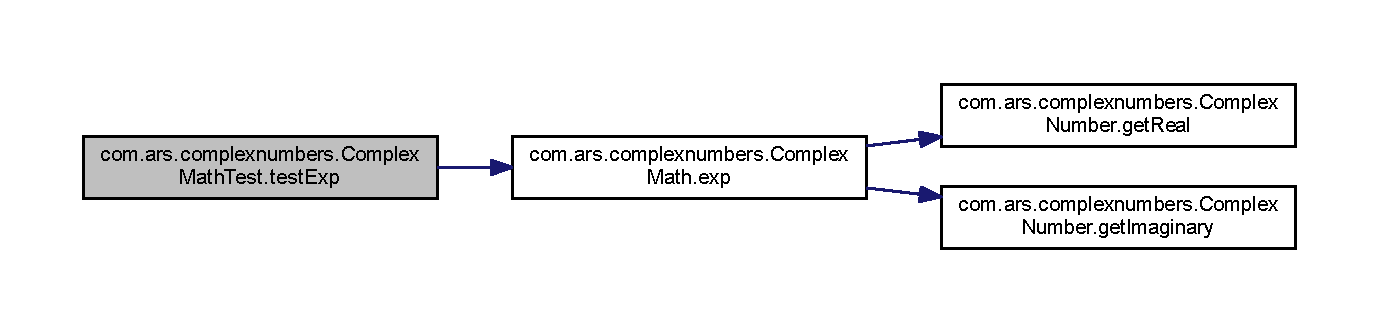
\includegraphics[width=350pt]{classcom_1_1ars_1_1complexnumbers_1_1_complex_math_test_abd1ea731d0875c3351306079e4694c24_cgraph}
\end{center}
\end{figure}
\hypertarget{classcom_1_1ars_1_1complexnumbers_1_1_complex_math_test_a2102465aa80b8303b2de77a3e87ffea9}{}\label{classcom_1_1ars_1_1complexnumbers_1_1_complex_math_test_a2102465aa80b8303b2de77a3e87ffea9} 
\index{com\+::ars\+::complexnumbers\+::\+Complex\+Math\+Test@{com\+::ars\+::complexnumbers\+::\+Complex\+Math\+Test}!test\+Get\+Arg@{test\+Get\+Arg}}
\index{test\+Get\+Arg@{test\+Get\+Arg}!com\+::ars\+::complexnumbers\+::\+Complex\+Math\+Test@{com\+::ars\+::complexnumbers\+::\+Complex\+Math\+Test}}
\subsubsection{\texorpdfstring{test\+Get\+Arg()}{testGetArg()}}
{\footnotesize\ttfamily void com.\+ars.\+complexnumbers.\+Complex\+Math\+Test.\+test\+Get\+Arg (\begin{DoxyParamCaption}{ }\end{DoxyParamCaption})}

Here is the call graph for this function\+:\nopagebreak
\begin{figure}[H]
\begin{center}
\leavevmode
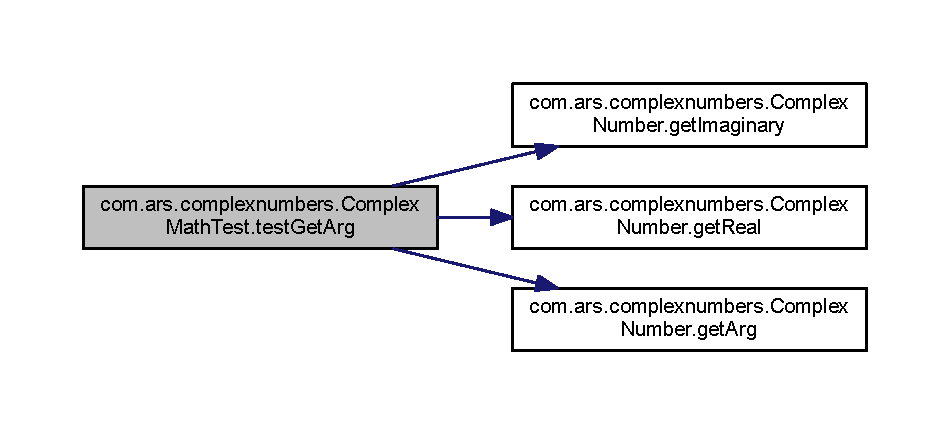
\includegraphics[width=350pt]{classcom_1_1ars_1_1complexnumbers_1_1_complex_math_test_a2102465aa80b8303b2de77a3e87ffea9_cgraph}
\end{center}
\end{figure}
\hypertarget{classcom_1_1ars_1_1complexnumbers_1_1_complex_math_test_a2c47b64252c4ecbe00d38fe89e66a9bb}{}\label{classcom_1_1ars_1_1complexnumbers_1_1_complex_math_test_a2c47b64252c4ecbe00d38fe89e66a9bb} 
\index{com\+::ars\+::complexnumbers\+::\+Complex\+Math\+Test@{com\+::ars\+::complexnumbers\+::\+Complex\+Math\+Test}!test\+Inverse@{test\+Inverse}}
\index{test\+Inverse@{test\+Inverse}!com\+::ars\+::complexnumbers\+::\+Complex\+Math\+Test@{com\+::ars\+::complexnumbers\+::\+Complex\+Math\+Test}}
\subsubsection{\texorpdfstring{test\+Inverse()}{testInverse()}}
{\footnotesize\ttfamily void com.\+ars.\+complexnumbers.\+Complex\+Math\+Test.\+test\+Inverse (\begin{DoxyParamCaption}{ }\end{DoxyParamCaption})}

Here is the call graph for this function\+:\nopagebreak
\begin{figure}[H]
\begin{center}
\leavevmode
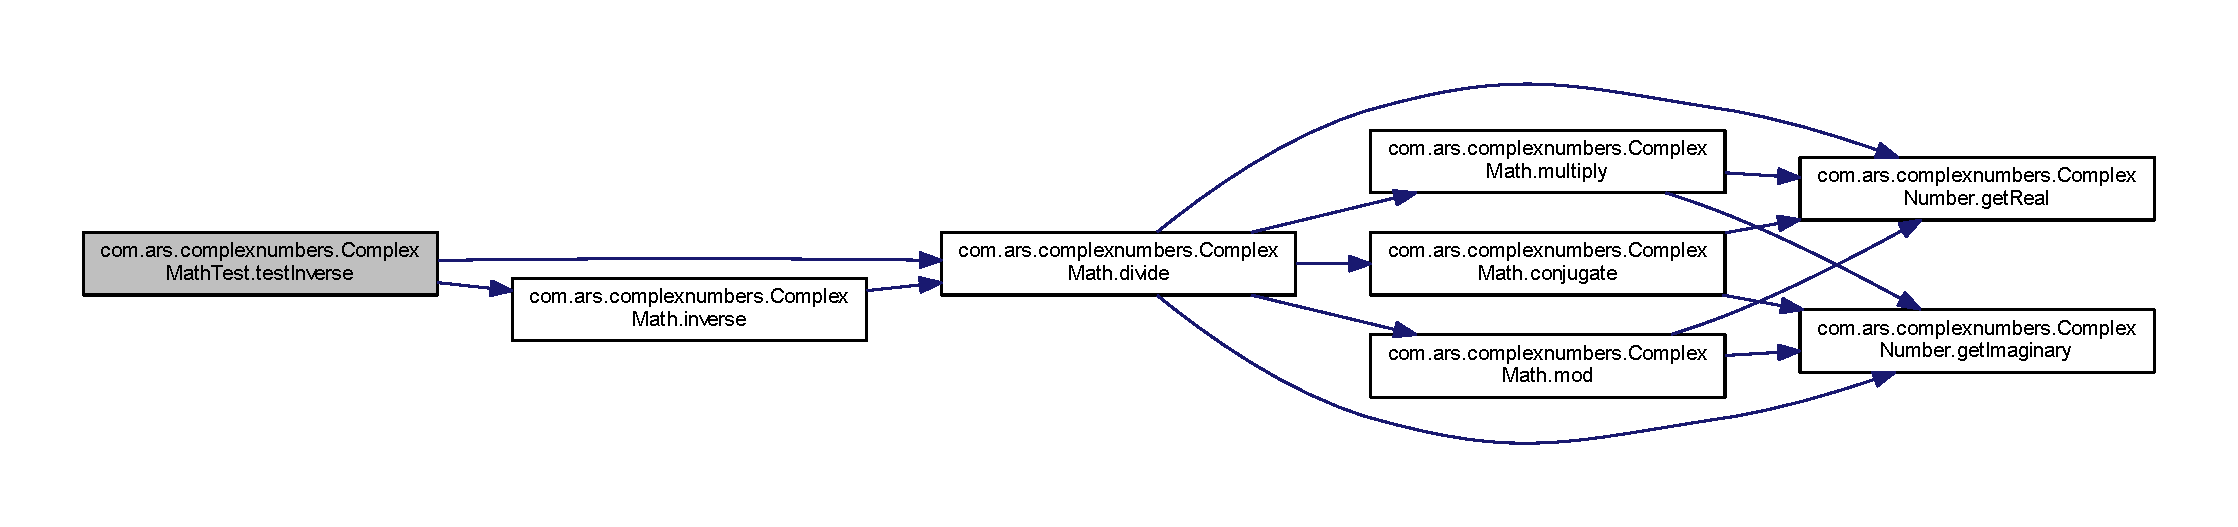
\includegraphics[width=350pt]{classcom_1_1ars_1_1complexnumbers_1_1_complex_math_test_a2c47b64252c4ecbe00d38fe89e66a9bb_cgraph}
\end{center}
\end{figure}
\hypertarget{classcom_1_1ars_1_1complexnumbers_1_1_complex_math_test_af1b3b844bab2323d1bd4bb07712f7652}{}\label{classcom_1_1ars_1_1complexnumbers_1_1_complex_math_test_af1b3b844bab2323d1bd4bb07712f7652} 
\index{com\+::ars\+::complexnumbers\+::\+Complex\+Math\+Test@{com\+::ars\+::complexnumbers\+::\+Complex\+Math\+Test}!test\+Mod@{test\+Mod}}
\index{test\+Mod@{test\+Mod}!com\+::ars\+::complexnumbers\+::\+Complex\+Math\+Test@{com\+::ars\+::complexnumbers\+::\+Complex\+Math\+Test}}
\subsubsection{\texorpdfstring{test\+Mod()}{testMod()}}
{\footnotesize\ttfamily void com.\+ars.\+complexnumbers.\+Complex\+Math\+Test.\+test\+Mod (\begin{DoxyParamCaption}{ }\end{DoxyParamCaption})}

Here is the call graph for this function\+:\nopagebreak
\begin{figure}[H]
\begin{center}
\leavevmode
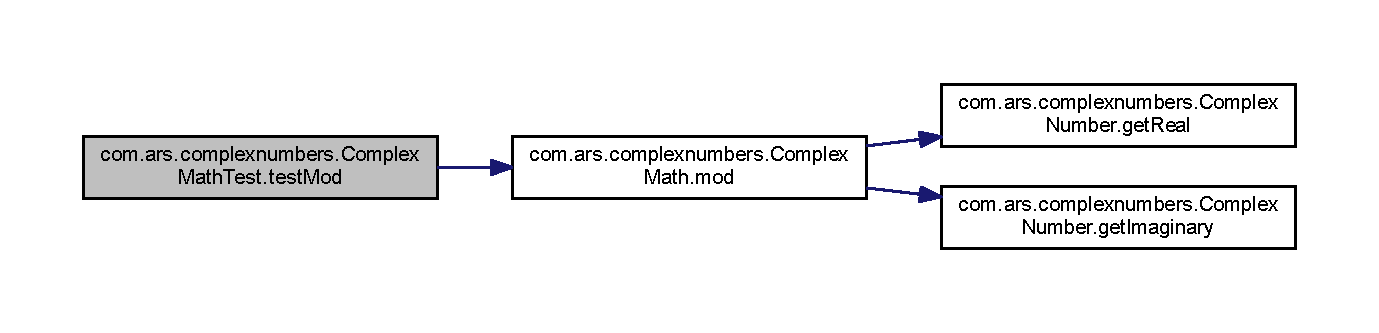
\includegraphics[width=350pt]{classcom_1_1ars_1_1complexnumbers_1_1_complex_math_test_af1b3b844bab2323d1bd4bb07712f7652_cgraph}
\end{center}
\end{figure}
\hypertarget{classcom_1_1ars_1_1complexnumbers_1_1_complex_math_test_a195e4c9c2b94ada809ff5ca462a9dc06}{}\label{classcom_1_1ars_1_1complexnumbers_1_1_complex_math_test_a195e4c9c2b94ada809ff5ca462a9dc06} 
\index{com\+::ars\+::complexnumbers\+::\+Complex\+Math\+Test@{com\+::ars\+::complexnumbers\+::\+Complex\+Math\+Test}!test\+Multiply@{test\+Multiply}}
\index{test\+Multiply@{test\+Multiply}!com\+::ars\+::complexnumbers\+::\+Complex\+Math\+Test@{com\+::ars\+::complexnumbers\+::\+Complex\+Math\+Test}}
\subsubsection{\texorpdfstring{test\+Multiply()}{testMultiply()}}
{\footnotesize\ttfamily void com.\+ars.\+complexnumbers.\+Complex\+Math\+Test.\+test\+Multiply (\begin{DoxyParamCaption}{ }\end{DoxyParamCaption})}

Here is the call graph for this function\+:\nopagebreak
\begin{figure}[H]
\begin{center}
\leavevmode
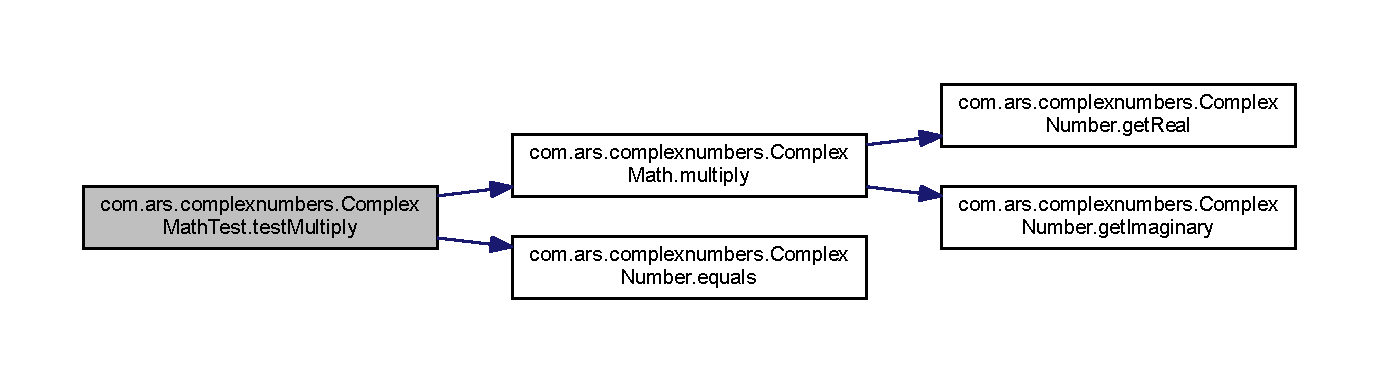
\includegraphics[width=350pt]{classcom_1_1ars_1_1complexnumbers_1_1_complex_math_test_a195e4c9c2b94ada809ff5ca462a9dc06_cgraph}
\end{center}
\end{figure}
\hypertarget{classcom_1_1ars_1_1complexnumbers_1_1_complex_math_test_a118231be2a26c23d165d3b40093352ac}{}\label{classcom_1_1ars_1_1complexnumbers_1_1_complex_math_test_a118231be2a26c23d165d3b40093352ac} 
\index{com\+::ars\+::complexnumbers\+::\+Complex\+Math\+Test@{com\+::ars\+::complexnumbers\+::\+Complex\+Math\+Test}!test\+Multiply\+Constant@{test\+Multiply\+Constant}}
\index{test\+Multiply\+Constant@{test\+Multiply\+Constant}!com\+::ars\+::complexnumbers\+::\+Complex\+Math\+Test@{com\+::ars\+::complexnumbers\+::\+Complex\+Math\+Test}}
\subsubsection{\texorpdfstring{test\+Multiply\+Constant()}{testMultiplyConstant()}}
{\footnotesize\ttfamily void com.\+ars.\+complexnumbers.\+Complex\+Math\+Test.\+test\+Multiply\+Constant (\begin{DoxyParamCaption}{ }\end{DoxyParamCaption})}

Here is the call graph for this function\+:\nopagebreak
\begin{figure}[H]
\begin{center}
\leavevmode
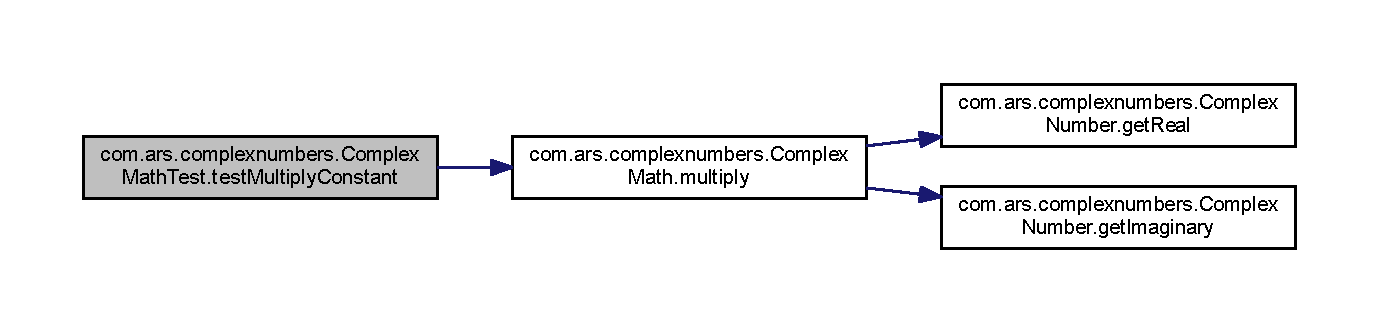
\includegraphics[width=350pt]{classcom_1_1ars_1_1complexnumbers_1_1_complex_math_test_a118231be2a26c23d165d3b40093352ac_cgraph}
\end{center}
\end{figure}
\hypertarget{classcom_1_1ars_1_1complexnumbers_1_1_complex_math_test_a70af211131478c43b06210fe524d3bd7}{}\label{classcom_1_1ars_1_1complexnumbers_1_1_complex_math_test_a70af211131478c43b06210fe524d3bd7} 
\index{com\+::ars\+::complexnumbers\+::\+Complex\+Math\+Test@{com\+::ars\+::complexnumbers\+::\+Complex\+Math\+Test}!test\+Pow@{test\+Pow}}
\index{test\+Pow@{test\+Pow}!com\+::ars\+::complexnumbers\+::\+Complex\+Math\+Test@{com\+::ars\+::complexnumbers\+::\+Complex\+Math\+Test}}
\subsubsection{\texorpdfstring{test\+Pow()}{testPow()}}
{\footnotesize\ttfamily void com.\+ars.\+complexnumbers.\+Complex\+Math\+Test.\+test\+Pow (\begin{DoxyParamCaption}{ }\end{DoxyParamCaption})}

Here is the call graph for this function\+:\nopagebreak
\begin{figure}[H]
\begin{center}
\leavevmode
\includegraphics[width=350pt]{classcom_1_1ars_1_1complexnumbers_1_1_complex_math_test_a70af211131478c43b06210fe524d3bd7_cgraph}
\end{center}
\end{figure}
\hypertarget{classcom_1_1ars_1_1complexnumbers_1_1_complex_math_test_ab429903cc819ea2c83369e07ba2f49e9}{}\label{classcom_1_1ars_1_1complexnumbers_1_1_complex_math_test_ab429903cc819ea2c83369e07ba2f49e9} 
\index{com\+::ars\+::complexnumbers\+::\+Complex\+Math\+Test@{com\+::ars\+::complexnumbers\+::\+Complex\+Math\+Test}!test\+Sine@{test\+Sine}}
\index{test\+Sine@{test\+Sine}!com\+::ars\+::complexnumbers\+::\+Complex\+Math\+Test@{com\+::ars\+::complexnumbers\+::\+Complex\+Math\+Test}}
\subsubsection{\texorpdfstring{test\+Sine()}{testSine()}}
{\footnotesize\ttfamily void com.\+ars.\+complexnumbers.\+Complex\+Math\+Test.\+test\+Sine (\begin{DoxyParamCaption}{ }\end{DoxyParamCaption})}

Here is the call graph for this function\+:\nopagebreak
\begin{figure}[H]
\begin{center}
\leavevmode
\includegraphics[width=350pt]{classcom_1_1ars_1_1complexnumbers_1_1_complex_math_test_ab429903cc819ea2c83369e07ba2f49e9_cgraph}
\end{center}
\end{figure}
\hypertarget{classcom_1_1ars_1_1complexnumbers_1_1_complex_math_test_a43dc686fe2b96e097f3ee8095fef12c1}{}\label{classcom_1_1ars_1_1complexnumbers_1_1_complex_math_test_a43dc686fe2b96e097f3ee8095fef12c1} 
\index{com\+::ars\+::complexnumbers\+::\+Complex\+Math\+Test@{com\+::ars\+::complexnumbers\+::\+Complex\+Math\+Test}!test\+Square@{test\+Square}}
\index{test\+Square@{test\+Square}!com\+::ars\+::complexnumbers\+::\+Complex\+Math\+Test@{com\+::ars\+::complexnumbers\+::\+Complex\+Math\+Test}}
\subsubsection{\texorpdfstring{test\+Square()}{testSquare()}}
{\footnotesize\ttfamily void com.\+ars.\+complexnumbers.\+Complex\+Math\+Test.\+test\+Square (\begin{DoxyParamCaption}{ }\end{DoxyParamCaption})}

Here is the call graph for this function\+:\nopagebreak
\begin{figure}[H]
\begin{center}
\leavevmode
\includegraphics[width=350pt]{classcom_1_1ars_1_1complexnumbers_1_1_complex_math_test_a43dc686fe2b96e097f3ee8095fef12c1_cgraph}
\end{center}
\end{figure}
\hypertarget{classcom_1_1ars_1_1complexnumbers_1_1_complex_math_test_a79e2b206d48588b1e7db17a681a405eb}{}\label{classcom_1_1ars_1_1complexnumbers_1_1_complex_math_test_a79e2b206d48588b1e7db17a681a405eb} 
\index{com\+::ars\+::complexnumbers\+::\+Complex\+Math\+Test@{com\+::ars\+::complexnumbers\+::\+Complex\+Math\+Test}!test\+Subtract@{test\+Subtract}}
\index{test\+Subtract@{test\+Subtract}!com\+::ars\+::complexnumbers\+::\+Complex\+Math\+Test@{com\+::ars\+::complexnumbers\+::\+Complex\+Math\+Test}}
\subsubsection{\texorpdfstring{test\+Subtract()}{testSubtract()}}
{\footnotesize\ttfamily void com.\+ars.\+complexnumbers.\+Complex\+Math\+Test.\+test\+Subtract (\begin{DoxyParamCaption}{ }\end{DoxyParamCaption})}

Here is the call graph for this function\+:\nopagebreak
\begin{figure}[H]
\begin{center}
\leavevmode
\includegraphics[width=350pt]{classcom_1_1ars_1_1complexnumbers_1_1_complex_math_test_a79e2b206d48588b1e7db17a681a405eb_cgraph}
\end{center}
\end{figure}
\hypertarget{classcom_1_1ars_1_1complexnumbers_1_1_complex_math_test_a535b2562407e9de2c6aea700d5e1a0f8}{}\label{classcom_1_1ars_1_1complexnumbers_1_1_complex_math_test_a535b2562407e9de2c6aea700d5e1a0f8} 
\index{com\+::ars\+::complexnumbers\+::\+Complex\+Math\+Test@{com\+::ars\+::complexnumbers\+::\+Complex\+Math\+Test}!test\+Subtract\+Constant@{test\+Subtract\+Constant}}
\index{test\+Subtract\+Constant@{test\+Subtract\+Constant}!com\+::ars\+::complexnumbers\+::\+Complex\+Math\+Test@{com\+::ars\+::complexnumbers\+::\+Complex\+Math\+Test}}
\subsubsection{\texorpdfstring{test\+Subtract\+Constant()}{testSubtractConstant()}}
{\footnotesize\ttfamily void com.\+ars.\+complexnumbers.\+Complex\+Math\+Test.\+test\+Subtract\+Constant (\begin{DoxyParamCaption}{ }\end{DoxyParamCaption})}

Here is the call graph for this function\+:\nopagebreak
\begin{figure}[H]
\begin{center}
\leavevmode
\includegraphics[width=350pt]{classcom_1_1ars_1_1complexnumbers_1_1_complex_math_test_a535b2562407e9de2c6aea700d5e1a0f8_cgraph}
\end{center}
\end{figure}
\hypertarget{classcom_1_1ars_1_1complexnumbers_1_1_complex_math_test_abcec8968bf43093a912ba2c24f4718a9}{}\label{classcom_1_1ars_1_1complexnumbers_1_1_complex_math_test_abcec8968bf43093a912ba2c24f4718a9} 
\index{com\+::ars\+::complexnumbers\+::\+Complex\+Math\+Test@{com\+::ars\+::complexnumbers\+::\+Complex\+Math\+Test}!test\+Tan@{test\+Tan}}
\index{test\+Tan@{test\+Tan}!com\+::ars\+::complexnumbers\+::\+Complex\+Math\+Test@{com\+::ars\+::complexnumbers\+::\+Complex\+Math\+Test}}
\subsubsection{\texorpdfstring{test\+Tan()}{testTan()}}
{\footnotesize\ttfamily void com.\+ars.\+complexnumbers.\+Complex\+Math\+Test.\+test\+Tan (\begin{DoxyParamCaption}{ }\end{DoxyParamCaption})}

Here is the call graph for this function\+:\nopagebreak
\begin{figure}[H]
\begin{center}
\leavevmode
\includegraphics[width=350pt]{classcom_1_1ars_1_1complexnumbers_1_1_complex_math_test_abcec8968bf43093a912ba2c24f4718a9_cgraph}
\end{center}
\end{figure}


The documentation for this class was generated from the following file\+:\begin{DoxyCompactItemize}
\item 
C\+:/\+Users/\+Dacian/\+Desktop/\+Quantum/\+Quantum/quantum\+\_\+computing-\/master/complexnumbers/src/test/java/com/ars/complexnumbers/\hyperlink{_complex_math_test_8java}{Complex\+Math\+Test.\+java}\end{DoxyCompactItemize}

\hypertarget{classcom_1_1ars_1_1complexnumbers_1_1_complex_number}{}\section{com.\+ars.\+complexnumbers.\+Complex\+Number Class Reference}
\label{classcom_1_1ars_1_1complexnumbers_1_1_complex_number}\index{com.\+ars.\+complexnumbers.\+Complex\+Number@{com.\+ars.\+complexnumbers.\+Complex\+Number}}
\subsection*{Public Member Functions}
\begin{DoxyCompactItemize}
\item 
\hyperlink{classcom_1_1ars_1_1complexnumbers_1_1_complex_number_a8798b32c39932a90436b5ef1d8bd83a4}{Complex\+Number} (double real, double imaginary)
\item 
\hyperlink{classcom_1_1ars_1_1complexnumbers_1_1_complex_number_a5c911c206c51fe7c3558e32147d22d12}{Complex\+Number} ()
\item 
void \hyperlink{classcom_1_1ars_1_1complexnumbers_1_1_complex_number_ac93a6120b2d6576dac75c256f0cd667f}{set} (double real, double imaginary)
\item 
void \hyperlink{classcom_1_1ars_1_1complexnumbers_1_1_complex_number_ae13ab597ac2208a3915398ee075a7b69}{set\+Real} (double real)
\item 
double \hyperlink{classcom_1_1ars_1_1complexnumbers_1_1_complex_number_a4cb4de35836a0ca818d3f2ce2df07736}{get\+Real} ()
\item 
double \hyperlink{classcom_1_1ars_1_1complexnumbers_1_1_complex_number_a611fa4712cc691cf1e13e91f182c1850}{get\+Imaginary} ()
\item 
void \hyperlink{classcom_1_1ars_1_1complexnumbers_1_1_complex_number_a728d224cd650d2e5ab62acd3159a4989}{set\+Imaginary} (double imaginary)
\item 
boolean \hyperlink{classcom_1_1ars_1_1complexnumbers_1_1_complex_number_a8dd0d197e07c92cb3f7e98697a18d96f}{equals} (Object o)
\item 
String \hyperlink{classcom_1_1ars_1_1complexnumbers_1_1_complex_number_ab55fe26ece82d837fc4db3ab88577aa0}{to\+String} ()
\item 
double \hyperlink{classcom_1_1ars_1_1complexnumbers_1_1_complex_number_a7cbe3a7d9d1e409b2c00cfd34e95b3e8}{get\+Arg} ()
\end{DoxyCompactItemize}


\subsection{Detailed Description}
\subsection*{\hyperlink{classcom_1_1ars_1_1complexnumbers_1_1_complex_number}{Complex\+Number}}

\hyperlink{classcom_1_1ars_1_1complexnumbers_1_1_complex_number}{Complex\+Number} class represents the data type for complex numbers.

\begin{DoxyAuthor}{Author}
Mihai Seba 
\end{DoxyAuthor}
\begin{DoxyVersion}{Version}
1.\+0 
\end{DoxyVersion}


\subsection{Constructor \& Destructor Documentation}
\hypertarget{classcom_1_1ars_1_1complexnumbers_1_1_complex_number_a8798b32c39932a90436b5ef1d8bd83a4}{}\label{classcom_1_1ars_1_1complexnumbers_1_1_complex_number_a8798b32c39932a90436b5ef1d8bd83a4} 
\index{com\+::ars\+::complexnumbers\+::\+Complex\+Number@{com\+::ars\+::complexnumbers\+::\+Complex\+Number}!Complex\+Number@{Complex\+Number}}
\index{Complex\+Number@{Complex\+Number}!com\+::ars\+::complexnumbers\+::\+Complex\+Number@{com\+::ars\+::complexnumbers\+::\+Complex\+Number}}
\subsubsection{\texorpdfstring{Complex\+Number()}{ComplexNumber()}\hspace{0.1cm}{\footnotesize\ttfamily [1/2]}}
{\footnotesize\ttfamily com.\+ars.\+complexnumbers.\+Complex\+Number.\+Complex\+Number (\begin{DoxyParamCaption}\item[{double}]{real,  }\item[{double}]{imaginary }\end{DoxyParamCaption})}

Constructs a new {\ttfamily \hyperlink{classcom_1_1ars_1_1complexnumbers_1_1_complex_number}{Complex\+Number}} object. 
\begin{DoxyParams}{Parameters}
{\em real} & the real part, Re(z), of the complex number \\
\hline
{\em imaginary} & the imaginary part, Im(z), of the complex number \\
\hline
\end{DoxyParams}
\hypertarget{classcom_1_1ars_1_1complexnumbers_1_1_complex_number_a5c911c206c51fe7c3558e32147d22d12}{}\label{classcom_1_1ars_1_1complexnumbers_1_1_complex_number_a5c911c206c51fe7c3558e32147d22d12} 
\index{com\+::ars\+::complexnumbers\+::\+Complex\+Number@{com\+::ars\+::complexnumbers\+::\+Complex\+Number}!Complex\+Number@{Complex\+Number}}
\index{Complex\+Number@{Complex\+Number}!com\+::ars\+::complexnumbers\+::\+Complex\+Number@{com\+::ars\+::complexnumbers\+::\+Complex\+Number}}
\subsubsection{\texorpdfstring{Complex\+Number()}{ComplexNumber()}\hspace{0.1cm}{\footnotesize\ttfamily [2/2]}}
{\footnotesize\ttfamily com.\+ars.\+complexnumbers.\+Complex\+Number.\+Complex\+Number (\begin{DoxyParamCaption}{ }\end{DoxyParamCaption})}

Constructs a new {\ttfamily \hyperlink{classcom_1_1ars_1_1complexnumbers_1_1_complex_number}{Complex\+Number}} object with both real and imaginary parts 0. 

\subsection{Member Function Documentation}
\hypertarget{classcom_1_1ars_1_1complexnumbers_1_1_complex_number_a8dd0d197e07c92cb3f7e98697a18d96f}{}\label{classcom_1_1ars_1_1complexnumbers_1_1_complex_number_a8dd0d197e07c92cb3f7e98697a18d96f} 
\index{com\+::ars\+::complexnumbers\+::\+Complex\+Number@{com\+::ars\+::complexnumbers\+::\+Complex\+Number}!equals@{equals}}
\index{equals@{equals}!com\+::ars\+::complexnumbers\+::\+Complex\+Number@{com\+::ars\+::complexnumbers\+::\+Complex\+Number}}
\subsubsection{\texorpdfstring{equals()}{equals()}}
{\footnotesize\ttfamily boolean com.\+ars.\+complexnumbers.\+Complex\+Number.\+equals (\begin{DoxyParamCaption}\item[{Object}]{o }\end{DoxyParamCaption})}

Check if passed {\ttfamily \hyperlink{classcom_1_1ars_1_1complexnumbers_1_1_complex_number}{Complex\+Number}} is equal to the current. 
\begin{DoxyParams}{Parameters}
{\em o} & the complex number to be checked \\
\hline
\end{DoxyParams}
\begin{DoxyReturn}{Returns}
true if the two complex numbers are equals, otherwise false 
\end{DoxyReturn}
Here is the caller graph for this function\+:\nopagebreak
\begin{figure}[H]
\begin{center}
\leavevmode
\includegraphics[width=350pt]{classcom_1_1ars_1_1complexnumbers_1_1_complex_number_a8dd0d197e07c92cb3f7e98697a18d96f_icgraph}
\end{center}
\end{figure}
\hypertarget{classcom_1_1ars_1_1complexnumbers_1_1_complex_number_a7cbe3a7d9d1e409b2c00cfd34e95b3e8}{}\label{classcom_1_1ars_1_1complexnumbers_1_1_complex_number_a7cbe3a7d9d1e409b2c00cfd34e95b3e8} 
\index{com\+::ars\+::complexnumbers\+::\+Complex\+Number@{com\+::ars\+::complexnumbers\+::\+Complex\+Number}!get\+Arg@{get\+Arg}}
\index{get\+Arg@{get\+Arg}!com\+::ars\+::complexnumbers\+::\+Complex\+Number@{com\+::ars\+::complexnumbers\+::\+Complex\+Number}}
\subsubsection{\texorpdfstring{get\+Arg()}{getArg()}}
{\footnotesize\ttfamily double com.\+ars.\+complexnumbers.\+Complex\+Number.\+get\+Arg (\begin{DoxyParamCaption}{ }\end{DoxyParamCaption})}

Calculates the argument of the current complex number. \begin{DoxyReturn}{Returns}
arg(z) the argument of the complex number. 
\end{DoxyReturn}
Here is the caller graph for this function\+:\nopagebreak
\begin{figure}[H]
\begin{center}
\leavevmode
\includegraphics[width=350pt]{classcom_1_1ars_1_1complexnumbers_1_1_complex_number_a7cbe3a7d9d1e409b2c00cfd34e95b3e8_icgraph}
\end{center}
\end{figure}
\hypertarget{classcom_1_1ars_1_1complexnumbers_1_1_complex_number_a611fa4712cc691cf1e13e91f182c1850}{}\label{classcom_1_1ars_1_1complexnumbers_1_1_complex_number_a611fa4712cc691cf1e13e91f182c1850} 
\index{com\+::ars\+::complexnumbers\+::\+Complex\+Number@{com\+::ars\+::complexnumbers\+::\+Complex\+Number}!get\+Imaginary@{get\+Imaginary}}
\index{get\+Imaginary@{get\+Imaginary}!com\+::ars\+::complexnumbers\+::\+Complex\+Number@{com\+::ars\+::complexnumbers\+::\+Complex\+Number}}
\subsubsection{\texorpdfstring{get\+Imaginary()}{getImaginary()}}
{\footnotesize\ttfamily double com.\+ars.\+complexnumbers.\+Complex\+Number.\+get\+Imaginary (\begin{DoxyParamCaption}{ }\end{DoxyParamCaption})}

Return the imaginary part of the complex number. \begin{DoxyReturn}{Returns}
Im(z), the imaginary part of the complex number 
\end{DoxyReturn}
Here is the caller graph for this function\+:
\nopagebreak
\begin{figure}[H]
\begin{center}
\leavevmode
\includegraphics[width=350pt]{classcom_1_1ars_1_1complexnumbers_1_1_complex_number_a611fa4712cc691cf1e13e91f182c1850_icgraph}
\end{center}
\end{figure}
\hypertarget{classcom_1_1ars_1_1complexnumbers_1_1_complex_number_a4cb4de35836a0ca818d3f2ce2df07736}{}\label{classcom_1_1ars_1_1complexnumbers_1_1_complex_number_a4cb4de35836a0ca818d3f2ce2df07736} 
\index{com\+::ars\+::complexnumbers\+::\+Complex\+Number@{com\+::ars\+::complexnumbers\+::\+Complex\+Number}!get\+Real@{get\+Real}}
\index{get\+Real@{get\+Real}!com\+::ars\+::complexnumbers\+::\+Complex\+Number@{com\+::ars\+::complexnumbers\+::\+Complex\+Number}}
\subsubsection{\texorpdfstring{get\+Real()}{getReal()}}
{\footnotesize\ttfamily double com.\+ars.\+complexnumbers.\+Complex\+Number.\+get\+Real (\begin{DoxyParamCaption}{ }\end{DoxyParamCaption})}

Return the real part of the complex number. \begin{DoxyReturn}{Returns}
Re(z), the real part of the complex number 
\end{DoxyReturn}
Here is the caller graph for this function\+:
\nopagebreak
\begin{figure}[H]
\begin{center}
\leavevmode
\includegraphics[width=350pt]{classcom_1_1ars_1_1complexnumbers_1_1_complex_number_a4cb4de35836a0ca818d3f2ce2df07736_icgraph}
\end{center}
\end{figure}
\hypertarget{classcom_1_1ars_1_1complexnumbers_1_1_complex_number_ac93a6120b2d6576dac75c256f0cd667f}{}\label{classcom_1_1ars_1_1complexnumbers_1_1_complex_number_ac93a6120b2d6576dac75c256f0cd667f} 
\index{com\+::ars\+::complexnumbers\+::\+Complex\+Number@{com\+::ars\+::complexnumbers\+::\+Complex\+Number}!set@{set}}
\index{set@{set}!com\+::ars\+::complexnumbers\+::\+Complex\+Number@{com\+::ars\+::complexnumbers\+::\+Complex\+Number}}
\subsubsection{\texorpdfstring{set()}{set()}}
{\footnotesize\ttfamily void com.\+ars.\+complexnumbers.\+Complex\+Number.\+set (\begin{DoxyParamCaption}\item[{double}]{real,  }\item[{double}]{imaginary }\end{DoxyParamCaption})}

Set the real and the imaginary part of the complex number. 
\begin{DoxyParams}{Parameters}
{\em real} & the real part, Re(z), of the complex number \\
\hline
{\em imaginary} & the imaginary,Im(z), of the complex number \\
\hline
\end{DoxyParams}
\hypertarget{classcom_1_1ars_1_1complexnumbers_1_1_complex_number_a728d224cd650d2e5ab62acd3159a4989}{}\label{classcom_1_1ars_1_1complexnumbers_1_1_complex_number_a728d224cd650d2e5ab62acd3159a4989} 
\index{com\+::ars\+::complexnumbers\+::\+Complex\+Number@{com\+::ars\+::complexnumbers\+::\+Complex\+Number}!set\+Imaginary@{set\+Imaginary}}
\index{set\+Imaginary@{set\+Imaginary}!com\+::ars\+::complexnumbers\+::\+Complex\+Number@{com\+::ars\+::complexnumbers\+::\+Complex\+Number}}
\subsubsection{\texorpdfstring{set\+Imaginary()}{setImaginary()}}
{\footnotesize\ttfamily void com.\+ars.\+complexnumbers.\+Complex\+Number.\+set\+Imaginary (\begin{DoxyParamCaption}\item[{double}]{imaginary }\end{DoxyParamCaption})}

Set the imaginary part of the complex number. 
\begin{DoxyParams}{Parameters}
{\em imaginary} & the imaginary part, Im(z), of the complex number \\
\hline
\end{DoxyParams}
Here is the caller graph for this function\+:
\nopagebreak
\begin{figure}[H]
\begin{center}
\leavevmode
\includegraphics[width=350pt]{classcom_1_1ars_1_1complexnumbers_1_1_complex_number_a728d224cd650d2e5ab62acd3159a4989_icgraph}
\end{center}
\end{figure}
\hypertarget{classcom_1_1ars_1_1complexnumbers_1_1_complex_number_ae13ab597ac2208a3915398ee075a7b69}{}\label{classcom_1_1ars_1_1complexnumbers_1_1_complex_number_ae13ab597ac2208a3915398ee075a7b69} 
\index{com\+::ars\+::complexnumbers\+::\+Complex\+Number@{com\+::ars\+::complexnumbers\+::\+Complex\+Number}!set\+Real@{set\+Real}}
\index{set\+Real@{set\+Real}!com\+::ars\+::complexnumbers\+::\+Complex\+Number@{com\+::ars\+::complexnumbers\+::\+Complex\+Number}}
\subsubsection{\texorpdfstring{set\+Real()}{setReal()}}
{\footnotesize\ttfamily void com.\+ars.\+complexnumbers.\+Complex\+Number.\+set\+Real (\begin{DoxyParamCaption}\item[{double}]{real }\end{DoxyParamCaption})}

Set the real part of the complex number. 
\begin{DoxyParams}{Parameters}
{\em real} & the real part, Re(z), of the complex number \\
\hline
\end{DoxyParams}
Here is the caller graph for this function\+:
\nopagebreak
\begin{figure}[H]
\begin{center}
\leavevmode
\includegraphics[width=350pt]{classcom_1_1ars_1_1complexnumbers_1_1_complex_number_ae13ab597ac2208a3915398ee075a7b69_icgraph}
\end{center}
\end{figure}
\hypertarget{classcom_1_1ars_1_1complexnumbers_1_1_complex_number_ab55fe26ece82d837fc4db3ab88577aa0}{}\label{classcom_1_1ars_1_1complexnumbers_1_1_complex_number_ab55fe26ece82d837fc4db3ab88577aa0} 
\index{com\+::ars\+::complexnumbers\+::\+Complex\+Number@{com\+::ars\+::complexnumbers\+::\+Complex\+Number}!to\+String@{to\+String}}
\index{to\+String@{to\+String}!com\+::ars\+::complexnumbers\+::\+Complex\+Number@{com\+::ars\+::complexnumbers\+::\+Complex\+Number}}
\subsubsection{\texorpdfstring{to\+String()}{toString()}}
{\footnotesize\ttfamily String com.\+ars.\+complexnumbers.\+Complex\+Number.\+to\+String (\begin{DoxyParamCaption}{ }\end{DoxyParamCaption})}

Return a string representation of the complex number. \begin{DoxyReturn}{Returns}
string the representation of the complex number 
\end{DoxyReturn}


The documentation for this class was generated from the following file\+:\begin{DoxyCompactItemize}
\item 
C\+:/\+Users/\+Dacian/\+Desktop/\+Quantum/\+Quantum/quantum\+\_\+computing-\/master/complexnumbers/src/main/java/com/ars/complexnumbers/\hyperlink{_complex_number_8java}{Complex\+Number.\+java}\end{DoxyCompactItemize}

\hypertarget{classcom_1_1ars_1_1quantumapp_1_1_deutsch_runner}{}\section{com.\+ars.\+quantumapp.\+Deutsch\+Runner Class Reference}
\label{classcom_1_1ars_1_1quantumapp_1_1_deutsch_runner}\index{com.\+ars.\+quantumapp.\+Deutsch\+Runner@{com.\+ars.\+quantumapp.\+Deutsch\+Runner}}


Inheritance diagram for com.\+ars.\+quantumapp.\+Deutsch\+Runner\+:\nopagebreak
\begin{figure}[H]
\begin{center}
\leavevmode
\includegraphics[width=227pt]{classcom_1_1ars_1_1quantumapp_1_1_deutsch_runner__inherit__graph}
\end{center}
\end{figure}


Collaboration diagram for com.\+ars.\+quantumapp.\+Deutsch\+Runner\+:\nopagebreak
\begin{figure}[H]
\begin{center}
\leavevmode
\includegraphics[width=227pt]{classcom_1_1ars_1_1quantumapp_1_1_deutsch_runner__coll__graph}
\end{center}
\end{figure}
\subsection*{Public Member Functions}
\begin{DoxyCompactItemize}
\item 
void \hyperlink{classcom_1_1ars_1_1quantumapp_1_1_deutsch_runner_a8dbef89cef296d4bb392f303e7c7ed85}{run} ()
\end{DoxyCompactItemize}


\subsection{Member Function Documentation}
\hypertarget{classcom_1_1ars_1_1quantumapp_1_1_deutsch_runner_a8dbef89cef296d4bb392f303e7c7ed85}{}\label{classcom_1_1ars_1_1quantumapp_1_1_deutsch_runner_a8dbef89cef296d4bb392f303e7c7ed85} 
\index{com\+::ars\+::quantumapp\+::\+Deutsch\+Runner@{com\+::ars\+::quantumapp\+::\+Deutsch\+Runner}!run@{run}}
\index{run@{run}!com\+::ars\+::quantumapp\+::\+Deutsch\+Runner@{com\+::ars\+::quantumapp\+::\+Deutsch\+Runner}}
\subsubsection{\texorpdfstring{run()}{run()}}
{\footnotesize\ttfamily void com.\+ars.\+quantumapp.\+Deutsch\+Runner.\+run (\begin{DoxyParamCaption}{ }\end{DoxyParamCaption})}



The documentation for this class was generated from the following file\+:\begin{DoxyCompactItemize}
\item 
C\+:/\+Users/\+Dacian/\+Desktop/\+Quantum/\+Quantum/quantum\+\_\+computing-\/master/quantumapp/src/main/java/com/ars/quantumapp/\hyperlink{_deutsch_runner_8java}{Deutsch\+Runner.\+java}\end{DoxyCompactItemize}

\hypertarget{classcom_1_1ars_1_1algorithms_1_1deutsch_1_1_deutschs_algorithm}{}\section{com.\+ars.\+algorithms.\+deutsch.\+Deutschs\+Algorithm Class Reference}
\label{classcom_1_1ars_1_1algorithms_1_1deutsch_1_1_deutschs_algorithm}\index{com.\+ars.\+algorithms.\+deutsch.\+Deutschs\+Algorithm@{com.\+ars.\+algorithms.\+deutsch.\+Deutschs\+Algorithm}}


Inheritance diagram for com.\+ars.\+algorithms.\+deutsch.\+Deutschs\+Algorithm\+:\nopagebreak
\begin{figure}[H]
\begin{center}
\leavevmode
\includegraphics[width=223pt]{classcom_1_1ars_1_1algorithms_1_1deutsch_1_1_deutschs_algorithm__inherit__graph}
\end{center}
\end{figure}


Collaboration diagram for com.\+ars.\+algorithms.\+deutsch.\+Deutschs\+Algorithm\+:
\nopagebreak
\begin{figure}[H]
\begin{center}
\leavevmode
\includegraphics[width=350pt]{classcom_1_1ars_1_1algorithms_1_1deutsch_1_1_deutschs_algorithm__coll__graph}
\end{center}
\end{figure}
\subsection*{Public Member Functions}
\begin{DoxyCompactItemize}
\item 
\hyperlink{classcom_1_1ars_1_1algorithms_1_1deutsch_1_1_deutschs_algorithm_a25599a3eb05e6bbf425692a3352462f6}{Deutschs\+Algorithm} (double\mbox{[}$\,$\mbox{]}\mbox{[}$\,$\mbox{]} tested\+Function\+Operator)
\item 
\hyperlink{classcom_1_1ars_1_1algorithms_1_1deutsch_1_1_deutschs_algorithm_a2908de89b7f76d8160272af477a1dc42}{Deutschs\+Algorithm} ()
\item 
void \hyperlink{classcom_1_1ars_1_1algorithms_1_1deutsch_1_1_deutschs_algorithm_a01537777ec24738faf83660313759ea4}{init} ()
\item 
void \hyperlink{classcom_1_1ars_1_1algorithms_1_1deutsch_1_1_deutschs_algorithm_afb9f22b5a65a36c5a2828e7f06e4563e}{run} ()
\item 
void \hyperlink{classcom_1_1ars_1_1algorithms_1_1deutsch_1_1_deutschs_algorithm_a205c99180da5c481f6733d07759de636}{measure} ()
\item 
boolean \hyperlink{classcom_1_1ars_1_1algorithms_1_1deutsch_1_1_deutschs_algorithm_a853d89cbac22f31c9b0fd24e53c3930d}{is\+Function\+Constant} ()
\item 
boolean \hyperlink{classcom_1_1ars_1_1algorithms_1_1deutsch_1_1_deutschs_algorithm_ad0d426fd3aa5441adb8892d9ccbe9705}{is\+Function\+Balanced} ()
\end{DoxyCompactItemize}
\subsection*{Additional Inherited Members}


\subsection{Constructor \& Destructor Documentation}
\hypertarget{classcom_1_1ars_1_1algorithms_1_1deutsch_1_1_deutschs_algorithm_a25599a3eb05e6bbf425692a3352462f6}{}\label{classcom_1_1ars_1_1algorithms_1_1deutsch_1_1_deutschs_algorithm_a25599a3eb05e6bbf425692a3352462f6} 
\index{com\+::ars\+::algorithms\+::deutsch\+::\+Deutschs\+Algorithm@{com\+::ars\+::algorithms\+::deutsch\+::\+Deutschs\+Algorithm}!Deutschs\+Algorithm@{Deutschs\+Algorithm}}
\index{Deutschs\+Algorithm@{Deutschs\+Algorithm}!com\+::ars\+::algorithms\+::deutsch\+::\+Deutschs\+Algorithm@{com\+::ars\+::algorithms\+::deutsch\+::\+Deutschs\+Algorithm}}
\subsubsection{\texorpdfstring{Deutschs\+Algorithm()}{DeutschsAlgorithm()}\hspace{0.1cm}{\footnotesize\ttfamily [1/2]}}
{\footnotesize\ttfamily com.\+ars.\+algorithms.\+deutsch.\+Deutschs\+Algorithm.\+Deutschs\+Algorithm (\begin{DoxyParamCaption}\item[{double}]{tested\+Function\+Operator\mbox{[}$\,$\mbox{]}\mbox{[}$\,$\mbox{]} }\end{DoxyParamCaption})}

\hypertarget{classcom_1_1ars_1_1algorithms_1_1deutsch_1_1_deutschs_algorithm_a2908de89b7f76d8160272af477a1dc42}{}\label{classcom_1_1ars_1_1algorithms_1_1deutsch_1_1_deutschs_algorithm_a2908de89b7f76d8160272af477a1dc42} 
\index{com\+::ars\+::algorithms\+::deutsch\+::\+Deutschs\+Algorithm@{com\+::ars\+::algorithms\+::deutsch\+::\+Deutschs\+Algorithm}!Deutschs\+Algorithm@{Deutschs\+Algorithm}}
\index{Deutschs\+Algorithm@{Deutschs\+Algorithm}!com\+::ars\+::algorithms\+::deutsch\+::\+Deutschs\+Algorithm@{com\+::ars\+::algorithms\+::deutsch\+::\+Deutschs\+Algorithm}}
\subsubsection{\texorpdfstring{Deutschs\+Algorithm()}{DeutschsAlgorithm()}\hspace{0.1cm}{\footnotesize\ttfamily [2/2]}}
{\footnotesize\ttfamily com.\+ars.\+algorithms.\+deutsch.\+Deutschs\+Algorithm.\+Deutschs\+Algorithm (\begin{DoxyParamCaption}{ }\end{DoxyParamCaption})}



\subsection{Member Function Documentation}
\hypertarget{classcom_1_1ars_1_1algorithms_1_1deutsch_1_1_deutschs_algorithm_a01537777ec24738faf83660313759ea4}{}\label{classcom_1_1ars_1_1algorithms_1_1deutsch_1_1_deutschs_algorithm_a01537777ec24738faf83660313759ea4} 
\index{com\+::ars\+::algorithms\+::deutsch\+::\+Deutschs\+Algorithm@{com\+::ars\+::algorithms\+::deutsch\+::\+Deutschs\+Algorithm}!init@{init}}
\index{init@{init}!com\+::ars\+::algorithms\+::deutsch\+::\+Deutschs\+Algorithm@{com\+::ars\+::algorithms\+::deutsch\+::\+Deutschs\+Algorithm}}
\subsubsection{\texorpdfstring{init()}{init()}}
{\footnotesize\ttfamily void com.\+ars.\+algorithms.\+deutsch.\+Deutschs\+Algorithm.\+init (\begin{DoxyParamCaption}{ }\end{DoxyParamCaption})}

Here is the call graph for this function\+:\nopagebreak
\begin{figure}[H]
\begin{center}
\leavevmode
\includegraphics[width=350pt]{classcom_1_1ars_1_1algorithms_1_1deutsch_1_1_deutschs_algorithm_a01537777ec24738faf83660313759ea4_cgraph}
\end{center}
\end{figure}
\hypertarget{classcom_1_1ars_1_1algorithms_1_1deutsch_1_1_deutschs_algorithm_ad0d426fd3aa5441adb8892d9ccbe9705}{}\label{classcom_1_1ars_1_1algorithms_1_1deutsch_1_1_deutschs_algorithm_ad0d426fd3aa5441adb8892d9ccbe9705} 
\index{com\+::ars\+::algorithms\+::deutsch\+::\+Deutschs\+Algorithm@{com\+::ars\+::algorithms\+::deutsch\+::\+Deutschs\+Algorithm}!is\+Function\+Balanced@{is\+Function\+Balanced}}
\index{is\+Function\+Balanced@{is\+Function\+Balanced}!com\+::ars\+::algorithms\+::deutsch\+::\+Deutschs\+Algorithm@{com\+::ars\+::algorithms\+::deutsch\+::\+Deutschs\+Algorithm}}
\subsubsection{\texorpdfstring{is\+Function\+Balanced()}{isFunctionBalanced()}}
{\footnotesize\ttfamily boolean com.\+ars.\+algorithms.\+deutsch.\+Deutschs\+Algorithm.\+is\+Function\+Balanced (\begin{DoxyParamCaption}{ }\end{DoxyParamCaption})}

Here is the call graph for this function\+:\nopagebreak
\begin{figure}[H]
\begin{center}
\leavevmode
\includegraphics[width=350pt]{classcom_1_1ars_1_1algorithms_1_1deutsch_1_1_deutschs_algorithm_ad0d426fd3aa5441adb8892d9ccbe9705_cgraph}
\end{center}
\end{figure}
\hypertarget{classcom_1_1ars_1_1algorithms_1_1deutsch_1_1_deutschs_algorithm_a853d89cbac22f31c9b0fd24e53c3930d}{}\label{classcom_1_1ars_1_1algorithms_1_1deutsch_1_1_deutschs_algorithm_a853d89cbac22f31c9b0fd24e53c3930d} 
\index{com\+::ars\+::algorithms\+::deutsch\+::\+Deutschs\+Algorithm@{com\+::ars\+::algorithms\+::deutsch\+::\+Deutschs\+Algorithm}!is\+Function\+Constant@{is\+Function\+Constant}}
\index{is\+Function\+Constant@{is\+Function\+Constant}!com\+::ars\+::algorithms\+::deutsch\+::\+Deutschs\+Algorithm@{com\+::ars\+::algorithms\+::deutsch\+::\+Deutschs\+Algorithm}}
\subsubsection{\texorpdfstring{is\+Function\+Constant()}{isFunctionConstant()}}
{\footnotesize\ttfamily boolean com.\+ars.\+algorithms.\+deutsch.\+Deutschs\+Algorithm.\+is\+Function\+Constant (\begin{DoxyParamCaption}{ }\end{DoxyParamCaption})}

Here is the call graph for this function\+:\nopagebreak
\begin{figure}[H]
\begin{center}
\leavevmode
\includegraphics[width=350pt]{classcom_1_1ars_1_1algorithms_1_1deutsch_1_1_deutschs_algorithm_a853d89cbac22f31c9b0fd24e53c3930d_cgraph}
\end{center}
\end{figure}
\hypertarget{classcom_1_1ars_1_1algorithms_1_1deutsch_1_1_deutschs_algorithm_a205c99180da5c481f6733d07759de636}{}\label{classcom_1_1ars_1_1algorithms_1_1deutsch_1_1_deutschs_algorithm_a205c99180da5c481f6733d07759de636} 
\index{com\+::ars\+::algorithms\+::deutsch\+::\+Deutschs\+Algorithm@{com\+::ars\+::algorithms\+::deutsch\+::\+Deutschs\+Algorithm}!measure@{measure}}
\index{measure@{measure}!com\+::ars\+::algorithms\+::deutsch\+::\+Deutschs\+Algorithm@{com\+::ars\+::algorithms\+::deutsch\+::\+Deutschs\+Algorithm}}
\subsubsection{\texorpdfstring{measure()}{measure()}}
{\footnotesize\ttfamily void com.\+ars.\+algorithms.\+deutsch.\+Deutschs\+Algorithm.\+measure (\begin{DoxyParamCaption}{ }\end{DoxyParamCaption})}

Here is the call graph for this function\+:\nopagebreak
\begin{figure}[H]
\begin{center}
\leavevmode
\includegraphics[width=350pt]{classcom_1_1ars_1_1algorithms_1_1deutsch_1_1_deutschs_algorithm_a205c99180da5c481f6733d07759de636_cgraph}
\end{center}
\end{figure}
\hypertarget{classcom_1_1ars_1_1algorithms_1_1deutsch_1_1_deutschs_algorithm_afb9f22b5a65a36c5a2828e7f06e4563e}{}\label{classcom_1_1ars_1_1algorithms_1_1deutsch_1_1_deutschs_algorithm_afb9f22b5a65a36c5a2828e7f06e4563e} 
\index{com\+::ars\+::algorithms\+::deutsch\+::\+Deutschs\+Algorithm@{com\+::ars\+::algorithms\+::deutsch\+::\+Deutschs\+Algorithm}!run@{run}}
\index{run@{run}!com\+::ars\+::algorithms\+::deutsch\+::\+Deutschs\+Algorithm@{com\+::ars\+::algorithms\+::deutsch\+::\+Deutschs\+Algorithm}}
\subsubsection{\texorpdfstring{run()}{run()}}
{\footnotesize\ttfamily void com.\+ars.\+algorithms.\+deutsch.\+Deutschs\+Algorithm.\+run (\begin{DoxyParamCaption}{ }\end{DoxyParamCaption})}

The following operations are performed\+: entangle qubit\+Zero (qubit\+Zero $\vert$$>$ gateX) $\vert$$>$ gate\+H2 $\vert$$>$ f $\vert$$>$ gate\+H2Here is the call graph for this function\+:\nopagebreak
\begin{figure}[H]
\begin{center}
\leavevmode
\includegraphics[width=350pt]{classcom_1_1ars_1_1algorithms_1_1deutsch_1_1_deutschs_algorithm_afb9f22b5a65a36c5a2828e7f06e4563e_cgraph}
\end{center}
\end{figure}


The documentation for this class was generated from the following file\+:\begin{DoxyCompactItemize}
\item 
C\+:/\+Users/\+Dacian/\+Desktop/\+Quantum/\+Quantum/quantum\+\_\+computing-\/master/quantum/src/main/java/com/ars/algorithms/deutsch/\hyperlink{_deutschs_algorithm_8java}{Deutschs\+Algorithm.\+java}\end{DoxyCompactItemize}

\hypertarget{enumcom_1_1ars_1_1gates_1_1_e_gate_types}{}\section{com.\+ars.\+gates.\+E\+Gate\+Types Enum Reference}
\label{enumcom_1_1ars_1_1gates_1_1_e_gate_types}\index{com.\+ars.\+gates.\+E\+Gate\+Types@{com.\+ars.\+gates.\+E\+Gate\+Types}}
\subsection*{Public Attributes}
\begin{DoxyCompactItemize}
\item 
\hyperlink{enumcom_1_1ars_1_1gates_1_1_e_gate_types_a374b473babbd584c22f80e6552064234}{E\+\_\+\+Toffoli\+Gate}
\item 
\hyperlink{enumcom_1_1ars_1_1gates_1_1_e_gate_types_abeb9ade3d4c04006200df8d2df685e67}{E\+\_\+\+Hadamard\+Gate}
\item 
\hyperlink{enumcom_1_1ars_1_1gates_1_1_e_gate_types_a4a07af93612467257717239122a1c03a}{E\+\_\+\+X\+Gate}
\item 
\hyperlink{enumcom_1_1ars_1_1gates_1_1_e_gate_types_ae9bf7c54ade9d79260e750bda4aec249}{E\+\_\+\+Z\+Gate}
\item 
\hyperlink{enumcom_1_1ars_1_1gates_1_1_e_gate_types_a921ebe3d6405141a79ae014d94445d48}{E\+\_\+\+C\+Not\+Gate}
\end{DoxyCompactItemize}


\subsection{Detailed Description}
Implemented Quantum Gates. 

\subsection{Member Data Documentation}
\hypertarget{enumcom_1_1ars_1_1gates_1_1_e_gate_types_a921ebe3d6405141a79ae014d94445d48}{}\label{enumcom_1_1ars_1_1gates_1_1_e_gate_types_a921ebe3d6405141a79ae014d94445d48} 
\index{com\+::ars\+::gates\+::\+E\+Gate\+Types@{com\+::ars\+::gates\+::\+E\+Gate\+Types}!E\+\_\+\+C\+Not\+Gate@{E\+\_\+\+C\+Not\+Gate}}
\index{E\+\_\+\+C\+Not\+Gate@{E\+\_\+\+C\+Not\+Gate}!com\+::ars\+::gates\+::\+E\+Gate\+Types@{com\+::ars\+::gates\+::\+E\+Gate\+Types}}
\subsubsection{\texorpdfstring{E\+\_\+\+C\+Not\+Gate}{E\_CNotGate}}
{\footnotesize\ttfamily com.\+ars.\+gates.\+E\+Gate\+Types.\+E\+\_\+\+C\+Not\+Gate}

C\+N\+OT Gate \hypertarget{enumcom_1_1ars_1_1gates_1_1_e_gate_types_abeb9ade3d4c04006200df8d2df685e67}{}\label{enumcom_1_1ars_1_1gates_1_1_e_gate_types_abeb9ade3d4c04006200df8d2df685e67} 
\index{com\+::ars\+::gates\+::\+E\+Gate\+Types@{com\+::ars\+::gates\+::\+E\+Gate\+Types}!E\+\_\+\+Hadamard\+Gate@{E\+\_\+\+Hadamard\+Gate}}
\index{E\+\_\+\+Hadamard\+Gate@{E\+\_\+\+Hadamard\+Gate}!com\+::ars\+::gates\+::\+E\+Gate\+Types@{com\+::ars\+::gates\+::\+E\+Gate\+Types}}
\subsubsection{\texorpdfstring{E\+\_\+\+Hadamard\+Gate}{E\_HadamardGate}}
{\footnotesize\ttfamily com.\+ars.\+gates.\+E\+Gate\+Types.\+E\+\_\+\+Hadamard\+Gate}

Hadamard Gate \hypertarget{enumcom_1_1ars_1_1gates_1_1_e_gate_types_a374b473babbd584c22f80e6552064234}{}\label{enumcom_1_1ars_1_1gates_1_1_e_gate_types_a374b473babbd584c22f80e6552064234} 
\index{com\+::ars\+::gates\+::\+E\+Gate\+Types@{com\+::ars\+::gates\+::\+E\+Gate\+Types}!E\+\_\+\+Toffoli\+Gate@{E\+\_\+\+Toffoli\+Gate}}
\index{E\+\_\+\+Toffoli\+Gate@{E\+\_\+\+Toffoli\+Gate}!com\+::ars\+::gates\+::\+E\+Gate\+Types@{com\+::ars\+::gates\+::\+E\+Gate\+Types}}
\subsubsection{\texorpdfstring{E\+\_\+\+Toffoli\+Gate}{E\_ToffoliGate}}
{\footnotesize\ttfamily com.\+ars.\+gates.\+E\+Gate\+Types.\+E\+\_\+\+Toffoli\+Gate}

Toffoli Gate \hypertarget{enumcom_1_1ars_1_1gates_1_1_e_gate_types_a4a07af93612467257717239122a1c03a}{}\label{enumcom_1_1ars_1_1gates_1_1_e_gate_types_a4a07af93612467257717239122a1c03a} 
\index{com\+::ars\+::gates\+::\+E\+Gate\+Types@{com\+::ars\+::gates\+::\+E\+Gate\+Types}!E\+\_\+\+X\+Gate@{E\+\_\+\+X\+Gate}}
\index{E\+\_\+\+X\+Gate@{E\+\_\+\+X\+Gate}!com\+::ars\+::gates\+::\+E\+Gate\+Types@{com\+::ars\+::gates\+::\+E\+Gate\+Types}}
\subsubsection{\texorpdfstring{E\+\_\+\+X\+Gate}{E\_XGate}}
{\footnotesize\ttfamily com.\+ars.\+gates.\+E\+Gate\+Types.\+E\+\_\+\+X\+Gate}

Pauli-\/X Gate \hypertarget{enumcom_1_1ars_1_1gates_1_1_e_gate_types_ae9bf7c54ade9d79260e750bda4aec249}{}\label{enumcom_1_1ars_1_1gates_1_1_e_gate_types_ae9bf7c54ade9d79260e750bda4aec249} 
\index{com\+::ars\+::gates\+::\+E\+Gate\+Types@{com\+::ars\+::gates\+::\+E\+Gate\+Types}!E\+\_\+\+Z\+Gate@{E\+\_\+\+Z\+Gate}}
\index{E\+\_\+\+Z\+Gate@{E\+\_\+\+Z\+Gate}!com\+::ars\+::gates\+::\+E\+Gate\+Types@{com\+::ars\+::gates\+::\+E\+Gate\+Types}}
\subsubsection{\texorpdfstring{E\+\_\+\+Z\+Gate}{E\_ZGate}}
{\footnotesize\ttfamily com.\+ars.\+gates.\+E\+Gate\+Types.\+E\+\_\+\+Z\+Gate}

Pauli-\/Z Gate 

The documentation for this enum was generated from the following file\+:\begin{DoxyCompactItemize}
\item 
C\+:/\+Users/\+Dacian/\+Desktop/\+Quantum/\+Quantum/quantum\+\_\+computing-\/master/quantum/src/main/java/com/ars/gates/\hyperlink{_e_gate_types_8java}{E\+Gate\+Types.\+java}\end{DoxyCompactItemize}

\hypertarget{classcom_1_1ars_1_1gates_1_1_gate_factory}{}\section{com.\+ars.\+gates.\+Gate\+Factory Class Reference}
\label{classcom_1_1ars_1_1gates_1_1_gate_factory}\index{com.\+ars.\+gates.\+Gate\+Factory@{com.\+ars.\+gates.\+Gate\+Factory}}


Inheritance diagram for com.\+ars.\+gates.\+Gate\+Factory\+:\nopagebreak
\begin{figure}[H]
\begin{center}
\leavevmode
\includegraphics[width=225pt]{classcom_1_1ars_1_1gates_1_1_gate_factory__inherit__graph}
\end{center}
\end{figure}


Collaboration diagram for com.\+ars.\+gates.\+Gate\+Factory\+:\nopagebreak
\begin{figure}[H]
\begin{center}
\leavevmode
\includegraphics[width=225pt]{classcom_1_1ars_1_1gates_1_1_gate_factory__coll__graph}
\end{center}
\end{figure}
\subsection*{Public Member Functions}
\begin{DoxyCompactItemize}
\item 
\hyperlink{interfacecom_1_1ars_1_1gates_1_1_i_gate}{I\+Gate} \hyperlink{classcom_1_1ars_1_1gates_1_1_gate_factory_a3a60759187c2a81cd1fec2ac7d3c847c}{get\+Gate} (\hyperlink{enumcom_1_1ars_1_1gates_1_1_e_gate_types}{E\+Gate\+Types} id)
\end{DoxyCompactItemize}


\subsection{Detailed Description}
Implementation of a Gate Factory. 

\subsection{Member Function Documentation}
\hypertarget{classcom_1_1ars_1_1gates_1_1_gate_factory_a3a60759187c2a81cd1fec2ac7d3c847c}{}\label{classcom_1_1ars_1_1gates_1_1_gate_factory_a3a60759187c2a81cd1fec2ac7d3c847c} 
\index{com\+::ars\+::gates\+::\+Gate\+Factory@{com\+::ars\+::gates\+::\+Gate\+Factory}!get\+Gate@{get\+Gate}}
\index{get\+Gate@{get\+Gate}!com\+::ars\+::gates\+::\+Gate\+Factory@{com\+::ars\+::gates\+::\+Gate\+Factory}}
\subsubsection{\texorpdfstring{get\+Gate()}{getGate()}}
{\footnotesize\ttfamily \hyperlink{interfacecom_1_1ars_1_1gates_1_1_i_gate}{I\+Gate} com.\+ars.\+gates.\+Gate\+Factory.\+get\+Gate (\begin{DoxyParamCaption}\item[{\hyperlink{enumcom_1_1ars_1_1gates_1_1_e_gate_types}{E\+Gate\+Types}}]{id }\end{DoxyParamCaption})}

get\+Gate return a new {\ttfamily Gate} object 
\begin{DoxyParams}{Parameters}
{\em id} & specify the type of gate. \\
\hline
\end{DoxyParams}
\begin{DoxyReturn}{Returns}
gate 
\end{DoxyReturn}


The documentation for this class was generated from the following file\+:\begin{DoxyCompactItemize}
\item 
C\+:/\+Users/\+Dacian/\+Desktop/\+Quantum/\+Quantum/quantum\+\_\+computing-\/master/quantum/src/main/java/com/ars/gates/\hyperlink{_gate_factory_8java}{Gate\+Factory.\+java}\end{DoxyCompactItemize}

\hypertarget{classcom_1_1ars_1_1gates_1_1_gate_producer}{}\section{com.\+ars.\+gates.\+Gate\+Producer Class Reference}
\label{classcom_1_1ars_1_1gates_1_1_gate_producer}\index{com.\+ars.\+gates.\+Gate\+Producer@{com.\+ars.\+gates.\+Gate\+Producer}}
\subsection*{Static Public Member Functions}
\begin{DoxyCompactItemize}
\item 
static \hyperlink{classcom_1_1ars_1_1gates_1_1_gates_abstract_factory}{Gates\+Abstract\+Factory} \hyperlink{classcom_1_1ars_1_1gates_1_1_gate_producer_a643829e30db1500430781afb9bc825e9}{get\+Gate\+Factory} ()
\end{DoxyCompactItemize}


\subsection{Detailed Description}
Implementation of Gate Producer. 

\subsection{Member Function Documentation}
\hypertarget{classcom_1_1ars_1_1gates_1_1_gate_producer_a643829e30db1500430781afb9bc825e9}{}\label{classcom_1_1ars_1_1gates_1_1_gate_producer_a643829e30db1500430781afb9bc825e9} 
\index{com\+::ars\+::gates\+::\+Gate\+Producer@{com\+::ars\+::gates\+::\+Gate\+Producer}!get\+Gate\+Factory@{get\+Gate\+Factory}}
\index{get\+Gate\+Factory@{get\+Gate\+Factory}!com\+::ars\+::gates\+::\+Gate\+Producer@{com\+::ars\+::gates\+::\+Gate\+Producer}}
\subsubsection{\texorpdfstring{get\+Gate\+Factory()}{getGateFactory()}}
{\footnotesize\ttfamily static \hyperlink{classcom_1_1ars_1_1gates_1_1_gates_abstract_factory}{Gates\+Abstract\+Factory} com.\+ars.\+gates.\+Gate\+Producer.\+get\+Gate\+Factory (\begin{DoxyParamCaption}{ }\end{DoxyParamCaption})\hspace{0.3cm}{\ttfamily [static]}}

Return a new {\ttfamily \hyperlink{classcom_1_1ars_1_1gates_1_1_gate_factory}{Gate\+Factory}} object. \begin{DoxyReturn}{Returns}
Gates\+Factory 
\end{DoxyReturn}
Here is the caller graph for this function\+:\nopagebreak
\begin{figure}[H]
\begin{center}
\leavevmode
\includegraphics[width=350pt]{classcom_1_1ars_1_1gates_1_1_gate_producer_a643829e30db1500430781afb9bc825e9_icgraph}
\end{center}
\end{figure}


The documentation for this class was generated from the following file\+:\begin{DoxyCompactItemize}
\item 
C\+:/\+Users/\+Dacian/\+Desktop/\+Quantum/\+Quantum/quantum\+\_\+computing-\/master/quantum/src/main/java/com/ars/gates/\hyperlink{_gate_producer_8java}{Gate\+Producer.\+java}\end{DoxyCompactItemize}

\hypertarget{classcom_1_1ars_1_1gates_1_1_gates_abstract_factory}{}\section{com.\+ars.\+gates.\+Gates\+Abstract\+Factory Class Reference}
\label{classcom_1_1ars_1_1gates_1_1_gates_abstract_factory}\index{com.\+ars.\+gates.\+Gates\+Abstract\+Factory@{com.\+ars.\+gates.\+Gates\+Abstract\+Factory}}


Inheritance diagram for com.\+ars.\+gates.\+Gates\+Abstract\+Factory\+:\nopagebreak
\begin{figure}[H]
\begin{center}
\leavevmode
\includegraphics[width=225pt]{classcom_1_1ars_1_1gates_1_1_gates_abstract_factory__inherit__graph}
\end{center}
\end{figure}
\subsection*{Public Member Functions}
\begin{DoxyCompactItemize}
\item 
abstract \hyperlink{interfacecom_1_1ars_1_1gates_1_1_i_gate}{I\+Gate} \hyperlink{classcom_1_1ars_1_1gates_1_1_gates_abstract_factory_a06a4a9da0a9fc741f70ce28b74156cab}{get\+Gate} (\hyperlink{enumcom_1_1ars_1_1gates_1_1_e_gate_types}{E\+Gate\+Types} id)
\end{DoxyCompactItemize}


\subsection{Detailed Description}
Implementation of a Abstract Factory 

\subsection{Member Function Documentation}
\hypertarget{classcom_1_1ars_1_1gates_1_1_gates_abstract_factory_a06a4a9da0a9fc741f70ce28b74156cab}{}\label{classcom_1_1ars_1_1gates_1_1_gates_abstract_factory_a06a4a9da0a9fc741f70ce28b74156cab} 
\index{com\+::ars\+::gates\+::\+Gates\+Abstract\+Factory@{com\+::ars\+::gates\+::\+Gates\+Abstract\+Factory}!get\+Gate@{get\+Gate}}
\index{get\+Gate@{get\+Gate}!com\+::ars\+::gates\+::\+Gates\+Abstract\+Factory@{com\+::ars\+::gates\+::\+Gates\+Abstract\+Factory}}
\subsubsection{\texorpdfstring{get\+Gate()}{getGate()}}
{\footnotesize\ttfamily abstract \hyperlink{interfacecom_1_1ars_1_1gates_1_1_i_gate}{I\+Gate} com.\+ars.\+gates.\+Gates\+Abstract\+Factory.\+get\+Gate (\begin{DoxyParamCaption}\item[{\hyperlink{enumcom_1_1ars_1_1gates_1_1_e_gate_types}{E\+Gate\+Types}}]{id }\end{DoxyParamCaption})\hspace{0.3cm}{\ttfamily [abstract]}}

Here is the caller graph for this function\+:
\nopagebreak
\begin{figure}[H]
\begin{center}
\leavevmode
\includegraphics[width=350pt]{classcom_1_1ars_1_1gates_1_1_gates_abstract_factory_a06a4a9da0a9fc741f70ce28b74156cab_icgraph}
\end{center}
\end{figure}


The documentation for this class was generated from the following file\+:\begin{DoxyCompactItemize}
\item 
C\+:/\+Users/\+Dacian/\+Desktop/\+Quantum/\+Quantum/quantum\+\_\+computing-\/master/quantum/src/main/java/com/ars/gates/\hyperlink{_gates_abstract_factory_8java}{Gates\+Abstract\+Factory.\+java}\end{DoxyCompactItemize}

\hypertarget{classcom_1_1ars_1_1quantumapp_1_1_grover_runner}{}\section{com.\+ars.\+quantumapp.\+Grover\+Runner Class Reference}
\label{classcom_1_1ars_1_1quantumapp_1_1_grover_runner}\index{com.\+ars.\+quantumapp.\+Grover\+Runner@{com.\+ars.\+quantumapp.\+Grover\+Runner}}


Inheritance diagram for com.\+ars.\+quantumapp.\+Grover\+Runner\+:\nopagebreak
\begin{figure}[H]
\begin{center}
\leavevmode
\includegraphics[width=219pt]{classcom_1_1ars_1_1quantumapp_1_1_grover_runner__inherit__graph}
\end{center}
\end{figure}


Collaboration diagram for com.\+ars.\+quantumapp.\+Grover\+Runner\+:\nopagebreak
\begin{figure}[H]
\begin{center}
\leavevmode
\includegraphics[width=219pt]{classcom_1_1ars_1_1quantumapp_1_1_grover_runner__coll__graph}
\end{center}
\end{figure}
\subsection*{Public Member Functions}
\begin{DoxyCompactItemize}
\item 
void \hyperlink{classcom_1_1ars_1_1quantumapp_1_1_grover_runner_a2524c67bd5ad4b1a33d613a4c12be738}{run} ()
\end{DoxyCompactItemize}


\subsection{Member Function Documentation}
\hypertarget{classcom_1_1ars_1_1quantumapp_1_1_grover_runner_a2524c67bd5ad4b1a33d613a4c12be738}{}\label{classcom_1_1ars_1_1quantumapp_1_1_grover_runner_a2524c67bd5ad4b1a33d613a4c12be738} 
\index{com\+::ars\+::quantumapp\+::\+Grover\+Runner@{com\+::ars\+::quantumapp\+::\+Grover\+Runner}!run@{run}}
\index{run@{run}!com\+::ars\+::quantumapp\+::\+Grover\+Runner@{com\+::ars\+::quantumapp\+::\+Grover\+Runner}}
\subsubsection{\texorpdfstring{run()}{run()}}
{\footnotesize\ttfamily void com.\+ars.\+quantumapp.\+Grover\+Runner.\+run (\begin{DoxyParamCaption}{ }\end{DoxyParamCaption})}

Here is the call graph for this function\+:\nopagebreak
\begin{figure}[H]
\begin{center}
\leavevmode
\includegraphics[width=350pt]{classcom_1_1ars_1_1quantumapp_1_1_grover_runner_a2524c67bd5ad4b1a33d613a4c12be738_cgraph}
\end{center}
\end{figure}


The documentation for this class was generated from the following file\+:\begin{DoxyCompactItemize}
\item 
C\+:/\+Users/\+Dacian/\+Desktop/\+Quantum/\+Quantum/quantum\+\_\+computing-\/master/quantumapp/src/main/java/com/ars/quantumapp/\hyperlink{_grover_runner_8java}{Grover\+Runner.\+java}\end{DoxyCompactItemize}

\hypertarget{classcom_1_1ars_1_1algorithms_1_1grover_1_1_grovers_algorithm}{}\section{com.\+ars.\+algorithms.\+grover.\+Grovers\+Algorithm Class Reference}
\label{classcom_1_1ars_1_1algorithms_1_1grover_1_1_grovers_algorithm}\index{com.\+ars.\+algorithms.\+grover.\+Grovers\+Algorithm@{com.\+ars.\+algorithms.\+grover.\+Grovers\+Algorithm}}


Inheritance diagram for com.\+ars.\+algorithms.\+grover.\+Grovers\+Algorithm\+:\nopagebreak
\begin{figure}[H]
\begin{center}
\leavevmode
\includegraphics[width=223pt]{classcom_1_1ars_1_1algorithms_1_1grover_1_1_grovers_algorithm__inherit__graph}
\end{center}
\end{figure}


Collaboration diagram for com.\+ars.\+algorithms.\+grover.\+Grovers\+Algorithm\+:
\nopagebreak
\begin{figure}[H]
\begin{center}
\leavevmode
\includegraphics[width=350pt]{classcom_1_1ars_1_1algorithms_1_1grover_1_1_grovers_algorithm__coll__graph}
\end{center}
\end{figure}
\subsection*{Public Member Functions}
\begin{DoxyCompactItemize}
\item 
\hyperlink{classcom_1_1ars_1_1algorithms_1_1grover_1_1_grovers_algorithm_acd86694e5d961a9e964a5dc439677738}{Grovers\+Algorithm} ()
\item 
void \hyperlink{classcom_1_1ars_1_1algorithms_1_1grover_1_1_grovers_algorithm_ae2825f36c10e6c822aef9da35992bef3}{init} ()
\item 
void \hyperlink{classcom_1_1ars_1_1algorithms_1_1grover_1_1_grovers_algorithm_a4b7b6a2e63a64325769a5ebeffb90ea9}{run} ()
\item 
void \hyperlink{classcom_1_1ars_1_1algorithms_1_1grover_1_1_grovers_algorithm_a8b5729e4882c27f2c4879bd2c7b6d17d}{measure} ()
\item 
void \hyperlink{classcom_1_1ars_1_1algorithms_1_1grover_1_1_grovers_algorithm_a0df6e611d65aed02934b95df8414fac0}{close} ()
\item 
void \hyperlink{classcom_1_1ars_1_1algorithms_1_1grover_1_1_grovers_algorithm_aaba2e3f570bd14cf35d8f81a0046075f}{create\+Oracle\+Matrix} ()
\end{DoxyCompactItemize}
\subsection*{Additional Inherited Members}


\subsection{Constructor \& Destructor Documentation}
\hypertarget{classcom_1_1ars_1_1algorithms_1_1grover_1_1_grovers_algorithm_acd86694e5d961a9e964a5dc439677738}{}\label{classcom_1_1ars_1_1algorithms_1_1grover_1_1_grovers_algorithm_acd86694e5d961a9e964a5dc439677738} 
\index{com\+::ars\+::algorithms\+::grover\+::\+Grovers\+Algorithm@{com\+::ars\+::algorithms\+::grover\+::\+Grovers\+Algorithm}!Grovers\+Algorithm@{Grovers\+Algorithm}}
\index{Grovers\+Algorithm@{Grovers\+Algorithm}!com\+::ars\+::algorithms\+::grover\+::\+Grovers\+Algorithm@{com\+::ars\+::algorithms\+::grover\+::\+Grovers\+Algorithm}}
\subsubsection{\texorpdfstring{Grovers\+Algorithm()}{GroversAlgorithm()}}
{\footnotesize\ttfamily com.\+ars.\+algorithms.\+grover.\+Grovers\+Algorithm.\+Grovers\+Algorithm (\begin{DoxyParamCaption}{ }\end{DoxyParamCaption})}

Here is the call graph for this function\+:\nopagebreak
\begin{figure}[H]
\begin{center}
\leavevmode
\includegraphics[width=350pt]{classcom_1_1ars_1_1algorithms_1_1grover_1_1_grovers_algorithm_acd86694e5d961a9e964a5dc439677738_cgraph}
\end{center}
\end{figure}


\subsection{Member Function Documentation}
\hypertarget{classcom_1_1ars_1_1algorithms_1_1grover_1_1_grovers_algorithm_a0df6e611d65aed02934b95df8414fac0}{}\label{classcom_1_1ars_1_1algorithms_1_1grover_1_1_grovers_algorithm_a0df6e611d65aed02934b95df8414fac0} 
\index{com\+::ars\+::algorithms\+::grover\+::\+Grovers\+Algorithm@{com\+::ars\+::algorithms\+::grover\+::\+Grovers\+Algorithm}!close@{close}}
\index{close@{close}!com\+::ars\+::algorithms\+::grover\+::\+Grovers\+Algorithm@{com\+::ars\+::algorithms\+::grover\+::\+Grovers\+Algorithm}}
\subsubsection{\texorpdfstring{close()}{close()}}
{\footnotesize\ttfamily void com.\+ars.\+algorithms.\+grover.\+Grovers\+Algorithm.\+close (\begin{DoxyParamCaption}{ }\end{DoxyParamCaption})}

Here is the caller graph for this function\+:\nopagebreak
\begin{figure}[H]
\begin{center}
\leavevmode
\includegraphics[width=350pt]{classcom_1_1ars_1_1algorithms_1_1grover_1_1_grovers_algorithm_a0df6e611d65aed02934b95df8414fac0_icgraph}
\end{center}
\end{figure}
\hypertarget{classcom_1_1ars_1_1algorithms_1_1grover_1_1_grovers_algorithm_aaba2e3f570bd14cf35d8f81a0046075f}{}\label{classcom_1_1ars_1_1algorithms_1_1grover_1_1_grovers_algorithm_aaba2e3f570bd14cf35d8f81a0046075f} 
\index{com\+::ars\+::algorithms\+::grover\+::\+Grovers\+Algorithm@{com\+::ars\+::algorithms\+::grover\+::\+Grovers\+Algorithm}!create\+Oracle\+Matrix@{create\+Oracle\+Matrix}}
\index{create\+Oracle\+Matrix@{create\+Oracle\+Matrix}!com\+::ars\+::algorithms\+::grover\+::\+Grovers\+Algorithm@{com\+::ars\+::algorithms\+::grover\+::\+Grovers\+Algorithm}}
\subsubsection{\texorpdfstring{create\+Oracle\+Matrix()}{createOracleMatrix()}}
{\footnotesize\ttfamily void com.\+ars.\+algorithms.\+grover.\+Grovers\+Algorithm.\+create\+Oracle\+Matrix (\begin{DoxyParamCaption}{ }\end{DoxyParamCaption})}

\hypertarget{classcom_1_1ars_1_1algorithms_1_1grover_1_1_grovers_algorithm_ae2825f36c10e6c822aef9da35992bef3}{}\label{classcom_1_1ars_1_1algorithms_1_1grover_1_1_grovers_algorithm_ae2825f36c10e6c822aef9da35992bef3} 
\index{com\+::ars\+::algorithms\+::grover\+::\+Grovers\+Algorithm@{com\+::ars\+::algorithms\+::grover\+::\+Grovers\+Algorithm}!init@{init}}
\index{init@{init}!com\+::ars\+::algorithms\+::grover\+::\+Grovers\+Algorithm@{com\+::ars\+::algorithms\+::grover\+::\+Grovers\+Algorithm}}
\subsubsection{\texorpdfstring{init()}{init()}}
{\footnotesize\ttfamily void com.\+ars.\+algorithms.\+grover.\+Grovers\+Algorithm.\+init (\begin{DoxyParamCaption}{ }\end{DoxyParamCaption})}

Here is the call graph for this function\+:\nopagebreak
\begin{figure}[H]
\begin{center}
\leavevmode
\includegraphics[width=350pt]{classcom_1_1ars_1_1algorithms_1_1grover_1_1_grovers_algorithm_ae2825f36c10e6c822aef9da35992bef3_cgraph}
\end{center}
\end{figure}
Here is the caller graph for this function\+:\nopagebreak
\begin{figure}[H]
\begin{center}
\leavevmode
\includegraphics[width=350pt]{classcom_1_1ars_1_1algorithms_1_1grover_1_1_grovers_algorithm_ae2825f36c10e6c822aef9da35992bef3_icgraph}
\end{center}
\end{figure}
\hypertarget{classcom_1_1ars_1_1algorithms_1_1grover_1_1_grovers_algorithm_a8b5729e4882c27f2c4879bd2c7b6d17d}{}\label{classcom_1_1ars_1_1algorithms_1_1grover_1_1_grovers_algorithm_a8b5729e4882c27f2c4879bd2c7b6d17d} 
\index{com\+::ars\+::algorithms\+::grover\+::\+Grovers\+Algorithm@{com\+::ars\+::algorithms\+::grover\+::\+Grovers\+Algorithm}!measure@{measure}}
\index{measure@{measure}!com\+::ars\+::algorithms\+::grover\+::\+Grovers\+Algorithm@{com\+::ars\+::algorithms\+::grover\+::\+Grovers\+Algorithm}}
\subsubsection{\texorpdfstring{measure()}{measure()}}
{\footnotesize\ttfamily void com.\+ars.\+algorithms.\+grover.\+Grovers\+Algorithm.\+measure (\begin{DoxyParamCaption}{ }\end{DoxyParamCaption})}

Here is the call graph for this function\+:\nopagebreak
\begin{figure}[H]
\begin{center}
\leavevmode
\includegraphics[width=350pt]{classcom_1_1ars_1_1algorithms_1_1grover_1_1_grovers_algorithm_a8b5729e4882c27f2c4879bd2c7b6d17d_cgraph}
\end{center}
\end{figure}
Here is the caller graph for this function\+:\nopagebreak
\begin{figure}[H]
\begin{center}
\leavevmode
\includegraphics[width=350pt]{classcom_1_1ars_1_1algorithms_1_1grover_1_1_grovers_algorithm_a8b5729e4882c27f2c4879bd2c7b6d17d_icgraph}
\end{center}
\end{figure}
\hypertarget{classcom_1_1ars_1_1algorithms_1_1grover_1_1_grovers_algorithm_a4b7b6a2e63a64325769a5ebeffb90ea9}{}\label{classcom_1_1ars_1_1algorithms_1_1grover_1_1_grovers_algorithm_a4b7b6a2e63a64325769a5ebeffb90ea9} 
\index{com\+::ars\+::algorithms\+::grover\+::\+Grovers\+Algorithm@{com\+::ars\+::algorithms\+::grover\+::\+Grovers\+Algorithm}!run@{run}}
\index{run@{run}!com\+::ars\+::algorithms\+::grover\+::\+Grovers\+Algorithm@{com\+::ars\+::algorithms\+::grover\+::\+Grovers\+Algorithm}}
\subsubsection{\texorpdfstring{run()}{run()}}
{\footnotesize\ttfamily void com.\+ars.\+algorithms.\+grover.\+Grovers\+Algorithm.\+run (\begin{DoxyParamCaption}{ }\end{DoxyParamCaption})}

Here is the call graph for this function\+:\nopagebreak
\begin{figure}[H]
\begin{center}
\leavevmode
\includegraphics[width=350pt]{classcom_1_1ars_1_1algorithms_1_1grover_1_1_grovers_algorithm_a4b7b6a2e63a64325769a5ebeffb90ea9_cgraph}
\end{center}
\end{figure}
Here is the caller graph for this function\+:\nopagebreak
\begin{figure}[H]
\begin{center}
\leavevmode
\includegraphics[width=350pt]{classcom_1_1ars_1_1algorithms_1_1grover_1_1_grovers_algorithm_a4b7b6a2e63a64325769a5ebeffb90ea9_icgraph}
\end{center}
\end{figure}


The documentation for this class was generated from the following file\+:\begin{DoxyCompactItemize}
\item 
C\+:/\+Users/\+Dacian/\+Desktop/\+Quantum/\+Quantum/quantum\+\_\+computing-\/master/quantum/src/main/java/com/ars/algorithms/grover/\hyperlink{_grovers_algorithm_8java}{Grovers\+Algorithm.\+java}\end{DoxyCompactItemize}

\hypertarget{classcom_1_1ars_1_1circuits_1_1_half_adder_cell}{}\section{com.\+ars.\+circuits.\+Half\+Adder\+Cell Class Reference}
\label{classcom_1_1ars_1_1circuits_1_1_half_adder_cell}\index{com.\+ars.\+circuits.\+Half\+Adder\+Cell@{com.\+ars.\+circuits.\+Half\+Adder\+Cell}}


Inheritance diagram for com.\+ars.\+circuits.\+Half\+Adder\+Cell\+:
\nopagebreak
\begin{figure}[H]
\begin{center}
\leavevmode
\includegraphics[width=228pt]{classcom_1_1ars_1_1circuits_1_1_half_adder_cell__inherit__graph}
\end{center}
\end{figure}


Collaboration diagram for com.\+ars.\+circuits.\+Half\+Adder\+Cell\+:
\nopagebreak
\begin{figure}[H]
\begin{center}
\leavevmode
\includegraphics[width=350pt]{classcom_1_1ars_1_1circuits_1_1_half_adder_cell__coll__graph}
\end{center}
\end{figure}
\subsection*{Public Member Functions}
\begin{DoxyCompactItemize}
\item 
double \mbox{[}$\,$\mbox{]}\mbox{[}$\,$\mbox{]} \hyperlink{classcom_1_1ars_1_1circuits_1_1_half_adder_cell_a540342262612af85393e1c07675fd7e9}{get\+Unitary\+Matrix} ()
\end{DoxyCompactItemize}
\subsection*{Protected Attributes}
\begin{DoxyCompactItemize}
\item 
\hyperlink{classcom_1_1ars_1_1gates_1_1_gates_abstract_factory}{Gates\+Abstract\+Factory} \hyperlink{classcom_1_1ars_1_1circuits_1_1_half_adder_cell_a5f7e032657ce1f64a8c735bac276653d}{gate\+Factory} = Gate\+Producer.\+get\+Gate\+Factory()
\end{DoxyCompactItemize}


\subsection{Member Function Documentation}
\hypertarget{classcom_1_1ars_1_1circuits_1_1_half_adder_cell_a540342262612af85393e1c07675fd7e9}{}\label{classcom_1_1ars_1_1circuits_1_1_half_adder_cell_a540342262612af85393e1c07675fd7e9} 
\index{com\+::ars\+::circuits\+::\+Half\+Adder\+Cell@{com\+::ars\+::circuits\+::\+Half\+Adder\+Cell}!get\+Unitary\+Matrix@{get\+Unitary\+Matrix}}
\index{get\+Unitary\+Matrix@{get\+Unitary\+Matrix}!com\+::ars\+::circuits\+::\+Half\+Adder\+Cell@{com\+::ars\+::circuits\+::\+Half\+Adder\+Cell}}
\subsubsection{\texorpdfstring{get\+Unitary\+Matrix()}{getUnitaryMatrix()}}
{\footnotesize\ttfamily double \mbox{[}$\,$\mbox{]}\mbox{[}$\,$\mbox{]} com.\+ars.\+circuits.\+Half\+Adder\+Cell.\+get\+Unitary\+Matrix (\begin{DoxyParamCaption}{ }\end{DoxyParamCaption})}



Implements \hyperlink{interfacecom_1_1ars_1_1circuits_1_1_i_circuit_a83a4a39c153cec6a292572228eaecbbc}{com.\+ars.\+circuits.\+I\+Circuit}.

Here is the call graph for this function\+:
\nopagebreak
\begin{figure}[H]
\begin{center}
\leavevmode
\includegraphics[width=350pt]{classcom_1_1ars_1_1circuits_1_1_half_adder_cell_a540342262612af85393e1c07675fd7e9_cgraph}
\end{center}
\end{figure}


\subsection{Member Data Documentation}
\hypertarget{classcom_1_1ars_1_1circuits_1_1_half_adder_cell_a5f7e032657ce1f64a8c735bac276653d}{}\label{classcom_1_1ars_1_1circuits_1_1_half_adder_cell_a5f7e032657ce1f64a8c735bac276653d} 
\index{com\+::ars\+::circuits\+::\+Half\+Adder\+Cell@{com\+::ars\+::circuits\+::\+Half\+Adder\+Cell}!gate\+Factory@{gate\+Factory}}
\index{gate\+Factory@{gate\+Factory}!com\+::ars\+::circuits\+::\+Half\+Adder\+Cell@{com\+::ars\+::circuits\+::\+Half\+Adder\+Cell}}
\subsubsection{\texorpdfstring{gate\+Factory}{gateFactory}}
{\footnotesize\ttfamily \hyperlink{classcom_1_1ars_1_1gates_1_1_gates_abstract_factory}{Gates\+Abstract\+Factory} com.\+ars.\+circuits.\+Half\+Adder\+Cell.\+gate\+Factory = Gate\+Producer.\+get\+Gate\+Factory()\hspace{0.3cm}{\ttfamily [protected]}}



The documentation for this class was generated from the following file\+:\begin{DoxyCompactItemize}
\item 
C\+:/\+Users/\+Dacian/\+Desktop/\+Quantum/\+Quantum/quantum\+\_\+computing-\/master/quantum/src/main/java/com/ars/circuits/\hyperlink{src_2main_2java_2com_2ars_2circuits_2_half_adder_cell_8java}{Half\+Adder\+Cell.\+java}\end{DoxyCompactItemize}

\hypertarget{classcom_1_1ars_1_1quantumapp_1_1_half_adder_cell}{}\section{com.\+ars.\+quantumapp.\+Half\+Adder\+Cell Class Reference}
\label{classcom_1_1ars_1_1quantumapp_1_1_half_adder_cell}\index{com.\+ars.\+quantumapp.\+Half\+Adder\+Cell@{com.\+ars.\+quantumapp.\+Half\+Adder\+Cell}}


Inheritance diagram for com.\+ars.\+quantumapp.\+Half\+Adder\+Cell\+:\nopagebreak
\begin{figure}[H]
\begin{center}
\leavevmode
\includegraphics[width=250pt]{classcom_1_1ars_1_1quantumapp_1_1_half_adder_cell__inherit__graph}
\end{center}
\end{figure}


Collaboration diagram for com.\+ars.\+quantumapp.\+Half\+Adder\+Cell\+:
\nopagebreak
\begin{figure}[H]
\begin{center}
\leavevmode
\includegraphics[width=350pt]{classcom_1_1ars_1_1quantumapp_1_1_half_adder_cell__coll__graph}
\end{center}
\end{figure}
\subsection*{Public Member Functions}
\begin{DoxyCompactItemize}
\item 
\hyperlink{classcom_1_1ars_1_1quantumapp_1_1_half_adder_cell_a9a5d3990c9d64a2480b990f2f32e86ed}{Half\+Adder\+Cell} (\hyperlink{classcom_1_1ars_1_1qubits_1_1_qubit}{Qubit} input\+Qubit\+X0, \hyperlink{classcom_1_1ars_1_1qubits_1_1_qubit}{Qubit} input\+Qubit\+X1, \hyperlink{classcom_1_1ars_1_1qubits_1_1_qubit}{Qubit} input\+Qubit\+Carry)
\item 
void \hyperlink{classcom_1_1ars_1_1quantumapp_1_1_half_adder_cell_a077ff8604fb9f4b2043ab4264327f4b4}{init} ()
\item 
void \hyperlink{classcom_1_1ars_1_1quantumapp_1_1_half_adder_cell_a2b0fc8424cf7d70048942436a3933917}{run} ()
\item 
void \hyperlink{classcom_1_1ars_1_1quantumapp_1_1_half_adder_cell_a534b92e8e8fd9cbc2538a4e86311b3aa}{measure} ()
\item 
void \hyperlink{classcom_1_1ars_1_1quantumapp_1_1_half_adder_cell_a9ce49c4de6b6267d794c9543e185e976}{close} ()
\end{DoxyCompactItemize}
\subsection*{Additional Inherited Members}


\subsection{Constructor \& Destructor Documentation}
\hypertarget{classcom_1_1ars_1_1quantumapp_1_1_half_adder_cell_a9a5d3990c9d64a2480b990f2f32e86ed}{}\label{classcom_1_1ars_1_1quantumapp_1_1_half_adder_cell_a9a5d3990c9d64a2480b990f2f32e86ed} 
\index{com\+::ars\+::quantumapp\+::\+Half\+Adder\+Cell@{com\+::ars\+::quantumapp\+::\+Half\+Adder\+Cell}!Half\+Adder\+Cell@{Half\+Adder\+Cell}}
\index{Half\+Adder\+Cell@{Half\+Adder\+Cell}!com\+::ars\+::quantumapp\+::\+Half\+Adder\+Cell@{com\+::ars\+::quantumapp\+::\+Half\+Adder\+Cell}}
\subsubsection{\texorpdfstring{Half\+Adder\+Cell()}{HalfAdderCell()}}
{\footnotesize\ttfamily com.\+ars.\+quantumapp.\+Half\+Adder\+Cell.\+Half\+Adder\+Cell (\begin{DoxyParamCaption}\item[{\hyperlink{classcom_1_1ars_1_1qubits_1_1_qubit}{Qubit}}]{input\+Qubit\+X0,  }\item[{\hyperlink{classcom_1_1ars_1_1qubits_1_1_qubit}{Qubit}}]{input\+Qubit\+X1,  }\item[{\hyperlink{classcom_1_1ars_1_1qubits_1_1_qubit}{Qubit}}]{input\+Qubit\+Carry }\end{DoxyParamCaption})}



\subsection{Member Function Documentation}
\hypertarget{classcom_1_1ars_1_1quantumapp_1_1_half_adder_cell_a9ce49c4de6b6267d794c9543e185e976}{}\label{classcom_1_1ars_1_1quantumapp_1_1_half_adder_cell_a9ce49c4de6b6267d794c9543e185e976} 
\index{com\+::ars\+::quantumapp\+::\+Half\+Adder\+Cell@{com\+::ars\+::quantumapp\+::\+Half\+Adder\+Cell}!close@{close}}
\index{close@{close}!com\+::ars\+::quantumapp\+::\+Half\+Adder\+Cell@{com\+::ars\+::quantumapp\+::\+Half\+Adder\+Cell}}
\subsubsection{\texorpdfstring{close()}{close()}}
{\footnotesize\ttfamily void com.\+ars.\+quantumapp.\+Half\+Adder\+Cell.\+close (\begin{DoxyParamCaption}{ }\end{DoxyParamCaption})}

\hypertarget{classcom_1_1ars_1_1quantumapp_1_1_half_adder_cell_a077ff8604fb9f4b2043ab4264327f4b4}{}\label{classcom_1_1ars_1_1quantumapp_1_1_half_adder_cell_a077ff8604fb9f4b2043ab4264327f4b4} 
\index{com\+::ars\+::quantumapp\+::\+Half\+Adder\+Cell@{com\+::ars\+::quantumapp\+::\+Half\+Adder\+Cell}!init@{init}}
\index{init@{init}!com\+::ars\+::quantumapp\+::\+Half\+Adder\+Cell@{com\+::ars\+::quantumapp\+::\+Half\+Adder\+Cell}}
\subsubsection{\texorpdfstring{init()}{init()}}
{\footnotesize\ttfamily void com.\+ars.\+quantumapp.\+Half\+Adder\+Cell.\+init (\begin{DoxyParamCaption}{ }\end{DoxyParamCaption})}

Here is the call graph for this function\+:\nopagebreak
\begin{figure}[H]
\begin{center}
\leavevmode
\includegraphics[width=350pt]{classcom_1_1ars_1_1quantumapp_1_1_half_adder_cell_a077ff8604fb9f4b2043ab4264327f4b4_cgraph}
\end{center}
\end{figure}
Here is the caller graph for this function\+:\nopagebreak
\begin{figure}[H]
\begin{center}
\leavevmode
\includegraphics[width=350pt]{classcom_1_1ars_1_1quantumapp_1_1_half_adder_cell_a077ff8604fb9f4b2043ab4264327f4b4_icgraph}
\end{center}
\end{figure}
\hypertarget{classcom_1_1ars_1_1quantumapp_1_1_half_adder_cell_a534b92e8e8fd9cbc2538a4e86311b3aa}{}\label{classcom_1_1ars_1_1quantumapp_1_1_half_adder_cell_a534b92e8e8fd9cbc2538a4e86311b3aa} 
\index{com\+::ars\+::quantumapp\+::\+Half\+Adder\+Cell@{com\+::ars\+::quantumapp\+::\+Half\+Adder\+Cell}!measure@{measure}}
\index{measure@{measure}!com\+::ars\+::quantumapp\+::\+Half\+Adder\+Cell@{com\+::ars\+::quantumapp\+::\+Half\+Adder\+Cell}}
\subsubsection{\texorpdfstring{measure()}{measure()}}
{\footnotesize\ttfamily void com.\+ars.\+quantumapp.\+Half\+Adder\+Cell.\+measure (\begin{DoxyParamCaption}{ }\end{DoxyParamCaption})}

Here is the call graph for this function\+:\nopagebreak
\begin{figure}[H]
\begin{center}
\leavevmode
\includegraphics[width=350pt]{classcom_1_1ars_1_1quantumapp_1_1_half_adder_cell_a534b92e8e8fd9cbc2538a4e86311b3aa_cgraph}
\end{center}
\end{figure}
Here is the caller graph for this function\+:\nopagebreak
\begin{figure}[H]
\begin{center}
\leavevmode
\includegraphics[width=350pt]{classcom_1_1ars_1_1quantumapp_1_1_half_adder_cell_a534b92e8e8fd9cbc2538a4e86311b3aa_icgraph}
\end{center}
\end{figure}
\hypertarget{classcom_1_1ars_1_1quantumapp_1_1_half_adder_cell_a2b0fc8424cf7d70048942436a3933917}{}\label{classcom_1_1ars_1_1quantumapp_1_1_half_adder_cell_a2b0fc8424cf7d70048942436a3933917} 
\index{com\+::ars\+::quantumapp\+::\+Half\+Adder\+Cell@{com\+::ars\+::quantumapp\+::\+Half\+Adder\+Cell}!run@{run}}
\index{run@{run}!com\+::ars\+::quantumapp\+::\+Half\+Adder\+Cell@{com\+::ars\+::quantumapp\+::\+Half\+Adder\+Cell}}
\subsubsection{\texorpdfstring{run()}{run()}}
{\footnotesize\ttfamily void com.\+ars.\+quantumapp.\+Half\+Adder\+Cell.\+run (\begin{DoxyParamCaption}{ }\end{DoxyParamCaption})}

Here is the call graph for this function\+:\nopagebreak
\begin{figure}[H]
\begin{center}
\leavevmode
\includegraphics[width=350pt]{classcom_1_1ars_1_1quantumapp_1_1_half_adder_cell_a2b0fc8424cf7d70048942436a3933917_cgraph}
\end{center}
\end{figure}
Here is the caller graph for this function\+:\nopagebreak
\begin{figure}[H]
\begin{center}
\leavevmode
\includegraphics[width=350pt]{classcom_1_1ars_1_1quantumapp_1_1_half_adder_cell_a2b0fc8424cf7d70048942436a3933917_icgraph}
\end{center}
\end{figure}


The documentation for this class was generated from the following file\+:\begin{DoxyCompactItemize}
\item 
C\+:/\+Users/\+Dacian/\+Desktop/\+Quantum/\+Quantum/quantum\+\_\+computing-\/master/quantumapp/src/main/java/com/ars/quantumapp/\hyperlink{pp_2src_2main_2java_2com_2ars_2quantumapp_2_half_adder_cell_8java}{Half\+Adder\+Cell.\+java}\end{DoxyCompactItemize}

\hypertarget{classcom_1_1ars_1_1quantumapp_1_1_half_adder_cell2}{}\section{com.\+ars.\+quantumapp.\+Half\+Adder\+Cell2 Class Reference}
\label{classcom_1_1ars_1_1quantumapp_1_1_half_adder_cell2}\index{com.\+ars.\+quantumapp.\+Half\+Adder\+Cell2@{com.\+ars.\+quantumapp.\+Half\+Adder\+Cell2}}


Inheritance diagram for com.\+ars.\+quantumapp.\+Half\+Adder\+Cell2\+:
\nopagebreak
\begin{figure}[H]
\begin{center}
\leavevmode
\includegraphics[width=233pt]{classcom_1_1ars_1_1quantumapp_1_1_half_adder_cell2__inherit__graph}
\end{center}
\end{figure}


Collaboration diagram for com.\+ars.\+quantumapp.\+Half\+Adder\+Cell2\+:
\nopagebreak
\begin{figure}[H]
\begin{center}
\leavevmode
\includegraphics[width=350pt]{classcom_1_1ars_1_1quantumapp_1_1_half_adder_cell2__coll__graph}
\end{center}
\end{figure}
\subsection*{Public Member Functions}
\begin{DoxyCompactItemize}
\item 
\hyperlink{classcom_1_1ars_1_1quantumapp_1_1_half_adder_cell2_a1369d2837b586d8e6076476b7ea03058}{Half\+Adder\+Cell2} (\hyperlink{classcom_1_1ars_1_1qubits_1_1_qubit}{Qubit} input\+Qubit\+X0, \hyperlink{classcom_1_1ars_1_1qubits_1_1_qubit}{Qubit} input\+Qubit\+X1, \hyperlink{classcom_1_1ars_1_1qubits_1_1_qubit}{Qubit} input\+Qubit\+Carry)
\item 
void \hyperlink{classcom_1_1ars_1_1quantumapp_1_1_half_adder_cell2_a9962ffb8cd54b25f0c696e7c06882195}{init} ()
\item 
void \hyperlink{classcom_1_1ars_1_1quantumapp_1_1_half_adder_cell2_a4552a018b3fdd228fb7d851be827754c}{run} ()
\item 
void \hyperlink{classcom_1_1ars_1_1quantumapp_1_1_half_adder_cell2_ace7018ecff35605ac317049d2584db13}{measure} ()
\end{DoxyCompactItemize}
\subsection*{Additional Inherited Members}


\subsection{Constructor \& Destructor Documentation}
\hypertarget{classcom_1_1ars_1_1quantumapp_1_1_half_adder_cell2_a1369d2837b586d8e6076476b7ea03058}{}\label{classcom_1_1ars_1_1quantumapp_1_1_half_adder_cell2_a1369d2837b586d8e6076476b7ea03058} 
\index{com\+::ars\+::quantumapp\+::\+Half\+Adder\+Cell2@{com\+::ars\+::quantumapp\+::\+Half\+Adder\+Cell2}!Half\+Adder\+Cell2@{Half\+Adder\+Cell2}}
\index{Half\+Adder\+Cell2@{Half\+Adder\+Cell2}!com\+::ars\+::quantumapp\+::\+Half\+Adder\+Cell2@{com\+::ars\+::quantumapp\+::\+Half\+Adder\+Cell2}}
\subsubsection{\texorpdfstring{Half\+Adder\+Cell2()}{HalfAdderCell2()}}
{\footnotesize\ttfamily com.\+ars.\+quantumapp.\+Half\+Adder\+Cell2.\+Half\+Adder\+Cell2 (\begin{DoxyParamCaption}\item[{\hyperlink{classcom_1_1ars_1_1qubits_1_1_qubit}{Qubit}}]{input\+Qubit\+X0,  }\item[{\hyperlink{classcom_1_1ars_1_1qubits_1_1_qubit}{Qubit}}]{input\+Qubit\+X1,  }\item[{\hyperlink{classcom_1_1ars_1_1qubits_1_1_qubit}{Qubit}}]{input\+Qubit\+Carry }\end{DoxyParamCaption})}



\subsection{Member Function Documentation}
\hypertarget{classcom_1_1ars_1_1quantumapp_1_1_half_adder_cell2_a9962ffb8cd54b25f0c696e7c06882195}{}\label{classcom_1_1ars_1_1quantumapp_1_1_half_adder_cell2_a9962ffb8cd54b25f0c696e7c06882195} 
\index{com\+::ars\+::quantumapp\+::\+Half\+Adder\+Cell2@{com\+::ars\+::quantumapp\+::\+Half\+Adder\+Cell2}!init@{init}}
\index{init@{init}!com\+::ars\+::quantumapp\+::\+Half\+Adder\+Cell2@{com\+::ars\+::quantumapp\+::\+Half\+Adder\+Cell2}}
\subsubsection{\texorpdfstring{init()}{init()}}
{\footnotesize\ttfamily void com.\+ars.\+quantumapp.\+Half\+Adder\+Cell2.\+init (\begin{DoxyParamCaption}{ }\end{DoxyParamCaption})}

Here is the call graph for this function\+:
\nopagebreak
\begin{figure}[H]
\begin{center}
\leavevmode
\includegraphics[width=350pt]{classcom_1_1ars_1_1quantumapp_1_1_half_adder_cell2_a9962ffb8cd54b25f0c696e7c06882195_cgraph}
\end{center}
\end{figure}
\hypertarget{classcom_1_1ars_1_1quantumapp_1_1_half_adder_cell2_ace7018ecff35605ac317049d2584db13}{}\label{classcom_1_1ars_1_1quantumapp_1_1_half_adder_cell2_ace7018ecff35605ac317049d2584db13} 
\index{com\+::ars\+::quantumapp\+::\+Half\+Adder\+Cell2@{com\+::ars\+::quantumapp\+::\+Half\+Adder\+Cell2}!measure@{measure}}
\index{measure@{measure}!com\+::ars\+::quantumapp\+::\+Half\+Adder\+Cell2@{com\+::ars\+::quantumapp\+::\+Half\+Adder\+Cell2}}
\subsubsection{\texorpdfstring{measure()}{measure()}}
{\footnotesize\ttfamily void com.\+ars.\+quantumapp.\+Half\+Adder\+Cell2.\+measure (\begin{DoxyParamCaption}{ }\end{DoxyParamCaption})}

Here is the call graph for this function\+:
\nopagebreak
\begin{figure}[H]
\begin{center}
\leavevmode
\includegraphics[width=350pt]{classcom_1_1ars_1_1quantumapp_1_1_half_adder_cell2_ace7018ecff35605ac317049d2584db13_cgraph}
\end{center}
\end{figure}
\hypertarget{classcom_1_1ars_1_1quantumapp_1_1_half_adder_cell2_a4552a018b3fdd228fb7d851be827754c}{}\label{classcom_1_1ars_1_1quantumapp_1_1_half_adder_cell2_a4552a018b3fdd228fb7d851be827754c} 
\index{com\+::ars\+::quantumapp\+::\+Half\+Adder\+Cell2@{com\+::ars\+::quantumapp\+::\+Half\+Adder\+Cell2}!run@{run}}
\index{run@{run}!com\+::ars\+::quantumapp\+::\+Half\+Adder\+Cell2@{com\+::ars\+::quantumapp\+::\+Half\+Adder\+Cell2}}
\subsubsection{\texorpdfstring{run()}{run()}}
{\footnotesize\ttfamily void com.\+ars.\+quantumapp.\+Half\+Adder\+Cell2.\+run (\begin{DoxyParamCaption}{ }\end{DoxyParamCaption})}

Here is the call graph for this function\+:
\nopagebreak
\begin{figure}[H]
\begin{center}
\leavevmode
\includegraphics[width=350pt]{classcom_1_1ars_1_1quantumapp_1_1_half_adder_cell2_a4552a018b3fdd228fb7d851be827754c_cgraph}
\end{center}
\end{figure}


The documentation for this class was generated from the following file\+:\begin{DoxyCompactItemize}
\item 
C\+:/\+Users/\+Dacian/\+Desktop/\+Quantum/\+Quantum/quantum\+\_\+computing-\/master/quantumapp/src/main/java/com/ars/quantumapp/\hyperlink{_half_adder_cell2_8java}{Half\+Adder\+Cell2.\+java}\end{DoxyCompactItemize}

\hypertarget{classcom_1_1ars_1_1quantumapp_1_1_half_adder_cell_runner}{}\section{com.\+ars.\+quantumapp.\+Half\+Adder\+Cell\+Runner Class Reference}
\label{classcom_1_1ars_1_1quantumapp_1_1_half_adder_cell_runner}\index{com.\+ars.\+quantumapp.\+Half\+Adder\+Cell\+Runner@{com.\+ars.\+quantumapp.\+Half\+Adder\+Cell\+Runner}}


Inheritance diagram for com.\+ars.\+quantumapp.\+Half\+Adder\+Cell\+Runner\+:\nopagebreak
\begin{figure}[H]
\begin{center}
\leavevmode
\includegraphics[width=233pt]{classcom_1_1ars_1_1quantumapp_1_1_half_adder_cell_runner__inherit__graph}
\end{center}
\end{figure}


Collaboration diagram for com.\+ars.\+quantumapp.\+Half\+Adder\+Cell\+Runner\+:\nopagebreak
\begin{figure}[H]
\begin{center}
\leavevmode
\includegraphics[width=233pt]{classcom_1_1ars_1_1quantumapp_1_1_half_adder_cell_runner__coll__graph}
\end{center}
\end{figure}
\subsection*{Public Member Functions}
\begin{DoxyCompactItemize}
\item 
void \hyperlink{classcom_1_1ars_1_1quantumapp_1_1_half_adder_cell_runner_a4f4ba989df2058187640a1868856c0c7}{run} ()
\end{DoxyCompactItemize}


\subsection{Member Function Documentation}
\hypertarget{classcom_1_1ars_1_1quantumapp_1_1_half_adder_cell_runner_a4f4ba989df2058187640a1868856c0c7}{}\label{classcom_1_1ars_1_1quantumapp_1_1_half_adder_cell_runner_a4f4ba989df2058187640a1868856c0c7} 
\index{com\+::ars\+::quantumapp\+::\+Half\+Adder\+Cell\+Runner@{com\+::ars\+::quantumapp\+::\+Half\+Adder\+Cell\+Runner}!run@{run}}
\index{run@{run}!com\+::ars\+::quantumapp\+::\+Half\+Adder\+Cell\+Runner@{com\+::ars\+::quantumapp\+::\+Half\+Adder\+Cell\+Runner}}
\subsubsection{\texorpdfstring{run()}{run()}}
{\footnotesize\ttfamily void com.\+ars.\+quantumapp.\+Half\+Adder\+Cell\+Runner.\+run (\begin{DoxyParamCaption}{ }\end{DoxyParamCaption})}

Here is the call graph for this function\+:\nopagebreak
\begin{figure}[H]
\begin{center}
\leavevmode
\includegraphics[width=350pt]{classcom_1_1ars_1_1quantumapp_1_1_half_adder_cell_runner_a4f4ba989df2058187640a1868856c0c7_cgraph}
\end{center}
\end{figure}


The documentation for this class was generated from the following file\+:\begin{DoxyCompactItemize}
\item 
C\+:/\+Users/\+Dacian/\+Desktop/\+Quantum/\+Quantum/quantum\+\_\+computing-\/master/quantumapp/src/main/java/com/ars/quantumapp/\hyperlink{_half_adder_cell_runner_8java}{Half\+Adder\+Cell\+Runner.\+java}\end{DoxyCompactItemize}

\hypertarget{classcom_1_1ars_1_1gates_1_1_h_gate}{}\section{com.\+ars.\+gates.\+H\+Gate Class Reference}
\label{classcom_1_1ars_1_1gates_1_1_h_gate}\index{com.\+ars.\+gates.\+H\+Gate@{com.\+ars.\+gates.\+H\+Gate}}


Inheritance diagram for com.\+ars.\+gates.\+H\+Gate\+:\nopagebreak
\begin{figure}[H]
\begin{center}
\leavevmode
\includegraphics[width=190pt]{classcom_1_1ars_1_1gates_1_1_h_gate__inherit__graph}
\end{center}
\end{figure}


Collaboration diagram for com.\+ars.\+gates.\+H\+Gate\+:\nopagebreak
\begin{figure}[H]
\begin{center}
\leavevmode
\includegraphics[width=190pt]{classcom_1_1ars_1_1gates_1_1_h_gate__coll__graph}
\end{center}
\end{figure}
\subsection*{Public Member Functions}
\begin{DoxyCompactItemize}
\item 
double \mbox{[}$\,$\mbox{]}\mbox{[}$\,$\mbox{]} \hyperlink{classcom_1_1ars_1_1gates_1_1_h_gate_a4749feb03fafcda241d9f854ef43a0d9}{get\+Unitary\+Matrix} ()
\end{DoxyCompactItemize}


\subsection{Detailed Description}
Implements the Hadamard Gate 

\subsection{Member Function Documentation}
\hypertarget{classcom_1_1ars_1_1gates_1_1_h_gate_a4749feb03fafcda241d9f854ef43a0d9}{}\label{classcom_1_1ars_1_1gates_1_1_h_gate_a4749feb03fafcda241d9f854ef43a0d9} 
\index{com\+::ars\+::gates\+::\+H\+Gate@{com\+::ars\+::gates\+::\+H\+Gate}!get\+Unitary\+Matrix@{get\+Unitary\+Matrix}}
\index{get\+Unitary\+Matrix@{get\+Unitary\+Matrix}!com\+::ars\+::gates\+::\+H\+Gate@{com\+::ars\+::gates\+::\+H\+Gate}}
\subsubsection{\texorpdfstring{get\+Unitary\+Matrix()}{getUnitaryMatrix()}}
{\footnotesize\ttfamily double \mbox{[}$\,$\mbox{]}\mbox{[}$\,$\mbox{]} com.\+ars.\+gates.\+H\+Gate.\+get\+Unitary\+Matrix (\begin{DoxyParamCaption}{ }\end{DoxyParamCaption})}

Return the 2D array corresponding to a Hadamard gate. \begin{DoxyReturn}{Returns}
double\mbox{[}\mbox{]}\mbox{[}\mbox{]} the corresponding 2D array 
\end{DoxyReturn}


Implements \hyperlink{interfacecom_1_1ars_1_1gates_1_1_i_gate_a6a940b3a6940cd97429aa211143121cb}{com.\+ars.\+gates.\+I\+Gate}.



The documentation for this class was generated from the following file\+:\begin{DoxyCompactItemize}
\item 
C\+:/\+Users/\+Dacian/\+Desktop/\+Quantum/\+Quantum/quantum\+\_\+computing-\/master/quantum/src/main/java/com/ars/gates/\hyperlink{_h_gate_8java}{H\+Gate.\+java}\end{DoxyCompactItemize}

\hypertarget{interfacecom_1_1ars_1_1circuits_1_1_i_circuit}{}\section{com.\+ars.\+circuits.\+I\+Circuit Interface Reference}
\label{interfacecom_1_1ars_1_1circuits_1_1_i_circuit}\index{com.\+ars.\+circuits.\+I\+Circuit@{com.\+ars.\+circuits.\+I\+Circuit}}


Inheritance diagram for com.\+ars.\+circuits.\+I\+Circuit\+:
\nopagebreak
\begin{figure}[H]
\begin{center}
\leavevmode
\includegraphics[width=228pt]{interfacecom_1_1ars_1_1circuits_1_1_i_circuit__inherit__graph}
\end{center}
\end{figure}
\subsection*{Public Member Functions}
\begin{DoxyCompactItemize}
\item 
double \mbox{[}$\,$\mbox{]}\mbox{[}$\,$\mbox{]} \hyperlink{interfacecom_1_1ars_1_1circuits_1_1_i_circuit_a83a4a39c153cec6a292572228eaecbbc}{get\+Unitary\+Matrix} ()
\end{DoxyCompactItemize}


\subsection{Member Function Documentation}
\hypertarget{interfacecom_1_1ars_1_1circuits_1_1_i_circuit_a83a4a39c153cec6a292572228eaecbbc}{}\label{interfacecom_1_1ars_1_1circuits_1_1_i_circuit_a83a4a39c153cec6a292572228eaecbbc} 
\index{com\+::ars\+::circuits\+::\+I\+Circuit@{com\+::ars\+::circuits\+::\+I\+Circuit}!get\+Unitary\+Matrix@{get\+Unitary\+Matrix}}
\index{get\+Unitary\+Matrix@{get\+Unitary\+Matrix}!com\+::ars\+::circuits\+::\+I\+Circuit@{com\+::ars\+::circuits\+::\+I\+Circuit}}
\subsubsection{\texorpdfstring{get\+Unitary\+Matrix()}{getUnitaryMatrix()}}
{\footnotesize\ttfamily double \mbox{[}$\,$\mbox{]}\mbox{[}$\,$\mbox{]} com.\+ars.\+circuits.\+I\+Circuit.\+get\+Unitary\+Matrix (\begin{DoxyParamCaption}{ }\end{DoxyParamCaption})}



Implemented in \hyperlink{classcom_1_1ars_1_1circuits_1_1_half_adder_cell_a540342262612af85393e1c07675fd7e9}{com.\+ars.\+circuits.\+Half\+Adder\+Cell}.

Here is the caller graph for this function\+:
\nopagebreak
\begin{figure}[H]
\begin{center}
\leavevmode
\includegraphics[width=350pt]{interfacecom_1_1ars_1_1circuits_1_1_i_circuit_a83a4a39c153cec6a292572228eaecbbc_icgraph}
\end{center}
\end{figure}


The documentation for this interface was generated from the following file\+:\begin{DoxyCompactItemize}
\item 
C\+:/\+Users/\+Dacian/\+Desktop/\+Quantum/\+Quantum/quantum\+\_\+computing-\/master/quantum/src/main/java/com/ars/circuits/\hyperlink{_i_circuit_8java}{I\+Circuit.\+java}\end{DoxyCompactItemize}

\hypertarget{interfacecom_1_1ars_1_1gates_1_1_i_gate}{}\section{com.\+ars.\+gates.\+I\+Gate Interface Reference}
\label{interfacecom_1_1ars_1_1gates_1_1_i_gate}\index{com.\+ars.\+gates.\+I\+Gate@{com.\+ars.\+gates.\+I\+Gate}}


Inheritance diagram for com.\+ars.\+gates.\+I\+Gate\+:\nopagebreak
\begin{figure}[H]
\begin{center}
\leavevmode
\includegraphics[width=350pt]{interfacecom_1_1ars_1_1gates_1_1_i_gate__inherit__graph}
\end{center}
\end{figure}
\subsection*{Public Member Functions}
\begin{DoxyCompactItemize}
\item 
double \mbox{[}$\,$\mbox{]}\mbox{[}$\,$\mbox{]} \hyperlink{interfacecom_1_1ars_1_1gates_1_1_i_gate_a6a940b3a6940cd97429aa211143121cb}{get\+Unitary\+Matrix} ()
\end{DoxyCompactItemize}


\subsection{Detailed Description}
Interface for all types of Quantum Gates. 

\subsection{Member Function Documentation}
\hypertarget{interfacecom_1_1ars_1_1gates_1_1_i_gate_a6a940b3a6940cd97429aa211143121cb}{}\label{interfacecom_1_1ars_1_1gates_1_1_i_gate_a6a940b3a6940cd97429aa211143121cb} 
\index{com\+::ars\+::gates\+::\+I\+Gate@{com\+::ars\+::gates\+::\+I\+Gate}!get\+Unitary\+Matrix@{get\+Unitary\+Matrix}}
\index{get\+Unitary\+Matrix@{get\+Unitary\+Matrix}!com\+::ars\+::gates\+::\+I\+Gate@{com\+::ars\+::gates\+::\+I\+Gate}}
\subsubsection{\texorpdfstring{get\+Unitary\+Matrix()}{getUnitaryMatrix()}}
{\footnotesize\ttfamily double \mbox{[}$\,$\mbox{]}\mbox{[}$\,$\mbox{]} com.\+ars.\+gates.\+I\+Gate.\+get\+Unitary\+Matrix (\begin{DoxyParamCaption}{ }\end{DoxyParamCaption})}



Implemented in \hyperlink{classcom_1_1ars_1_1gates_1_1_wiggle_gate_a1007dd60c814cd64bb6abbd8c3b9e409}{com.\+ars.\+gates.\+Wiggle\+Gate}, \hyperlink{classcom_1_1ars_1_1gates_1_1_h_gate_a4749feb03fafcda241d9f854ef43a0d9}{com.\+ars.\+gates.\+H\+Gate}, \hyperlink{classcom_1_1ars_1_1gates_1_1_x_gate_aa0e495ad8fa7fd0e23ecea6f01c02f6e}{com.\+ars.\+gates.\+X\+Gate}, \hyperlink{classcom_1_1ars_1_1gates_1_1_z_gate_a1009d3144a50f50332e64b6e7f37b578}{com.\+ars.\+gates.\+Z\+Gate}, \hyperlink{classcom_1_1ars_1_1gates_1_1_c_not_gate_a3a78f3ef3d7a418a51b3fabc46954ec5}{com.\+ars.\+gates.\+C\+Not\+Gate}, and \hyperlink{classcom_1_1ars_1_1gates_1_1_toffoli_gate_a0c253237312f11c98ffea807d63f925c}{com.\+ars.\+gates.\+Toffoli\+Gate}.

Here is the caller graph for this function\+:
\nopagebreak
\begin{figure}[H]
\begin{center}
\leavevmode
\includegraphics[width=350pt]{interfacecom_1_1ars_1_1gates_1_1_i_gate_a6a940b3a6940cd97429aa211143121cb_icgraph}
\end{center}
\end{figure}


The documentation for this interface was generated from the following file\+:\begin{DoxyCompactItemize}
\item 
C\+:/\+Users/\+Dacian/\+Desktop/\+Quantum/\+Quantum/quantum\+\_\+computing-\/master/quantum/src/main/java/com/ars/gates/\hyperlink{_i_gate_8java}{I\+Gate.\+java}\end{DoxyCompactItemize}

\hypertarget{classcom_1_1ars_1_1quantum_1_1utils_1_1_matrix_operations}{}\section{com.\+ars.\+quantum.\+utils.\+Matrix\+Operations Class Reference}
\label{classcom_1_1ars_1_1quantum_1_1utils_1_1_matrix_operations}\index{com.\+ars.\+quantum.\+utils.\+Matrix\+Operations@{com.\+ars.\+quantum.\+utils.\+Matrix\+Operations}}
\subsection*{Classes}
\begin{DoxyCompactItemize}
\item 
class {\bfseries Incorrect\+Matrix\+Size\+Exception}
\end{DoxyCompactItemize}
\subsection*{Static Public Member Functions}
\begin{DoxyCompactItemize}
\item 
static double \mbox{[}$\,$\mbox{]}\mbox{[}$\,$\mbox{]} \hyperlink{classcom_1_1ars_1_1quantum_1_1utils_1_1_matrix_operations_a0739b9c18cbe7d85ae01056f4b7e08d9}{multiply} (double\mbox{[}$\,$\mbox{]}\mbox{[}$\,$\mbox{]} a, double\mbox{[}$\,$\mbox{]}\mbox{[}$\,$\mbox{]} b)  throws Incorrect\+Matrix\+Size\+Exception 
\item 
static \hyperlink{classcom_1_1ars_1_1complexnumbers_1_1_complex_number}{Complex\+Number} \mbox{[}$\,$\mbox{]}\mbox{[}$\,$\mbox{]} \hyperlink{classcom_1_1ars_1_1quantum_1_1utils_1_1_matrix_operations_ae7c98406e2a3c1d35d78538d82bd637d}{multiply} (\hyperlink{classcom_1_1ars_1_1complexnumbers_1_1_complex_number}{Complex\+Number}\mbox{[}$\,$\mbox{]}\mbox{[}$\,$\mbox{]} a, \hyperlink{classcom_1_1ars_1_1complexnumbers_1_1_complex_number}{Complex\+Number}\mbox{[}$\,$\mbox{]}\mbox{[}$\,$\mbox{]} b)  throws Incorrect\+Matrix\+Size\+Exception 
\item 
static double \mbox{[}$\,$\mbox{]}\mbox{[}$\,$\mbox{]} \hyperlink{classcom_1_1ars_1_1quantum_1_1utils_1_1_matrix_operations_af6e0ec44a13d9a89b249606514378bf8}{add} (double\mbox{[}$\,$\mbox{]}\mbox{[}$\,$\mbox{]} a, double\mbox{[}$\,$\mbox{]}\mbox{[}$\,$\mbox{]} b)  throws Incorrect\+Matrix\+Size\+Exception 
\item 
static \hyperlink{classcom_1_1ars_1_1complexnumbers_1_1_complex_number}{Complex\+Number} \mbox{[}$\,$\mbox{]}\mbox{[}$\,$\mbox{]} \hyperlink{classcom_1_1ars_1_1quantum_1_1utils_1_1_matrix_operations_aa9b253355d52423992f5208ff2d72b15}{add} (\hyperlink{classcom_1_1ars_1_1complexnumbers_1_1_complex_number}{Complex\+Number}\mbox{[}$\,$\mbox{]}\mbox{[}$\,$\mbox{]} a, \hyperlink{classcom_1_1ars_1_1complexnumbers_1_1_complex_number}{Complex\+Number}\mbox{[}$\,$\mbox{]}\mbox{[}$\,$\mbox{]} b)  throws Incorrect\+Matrix\+Size\+Exception 
\item 
static double \mbox{[}$\,$\mbox{]}\mbox{[}$\,$\mbox{]} \hyperlink{classcom_1_1ars_1_1quantum_1_1utils_1_1_matrix_operations_a7ccc1120dba8158f6cb778ad6a55927d}{subtract} (double\mbox{[}$\,$\mbox{]}\mbox{[}$\,$\mbox{]} a, double\mbox{[}$\,$\mbox{]}\mbox{[}$\,$\mbox{]} b)  throws Incorrect\+Matrix\+Size\+Exception 
\item 
static \hyperlink{classcom_1_1ars_1_1complexnumbers_1_1_complex_number}{Complex\+Number} \mbox{[}$\,$\mbox{]}\mbox{[}$\,$\mbox{]} \hyperlink{classcom_1_1ars_1_1quantum_1_1utils_1_1_matrix_operations_a99b64f57485b148b298a3a7e08c002f6}{subtract} (\hyperlink{classcom_1_1ars_1_1complexnumbers_1_1_complex_number}{Complex\+Number}\mbox{[}$\,$\mbox{]}\mbox{[}$\,$\mbox{]} a, \hyperlink{classcom_1_1ars_1_1complexnumbers_1_1_complex_number}{Complex\+Number}\mbox{[}$\,$\mbox{]}\mbox{[}$\,$\mbox{]} b)  throws Incorrect\+Matrix\+Size\+Exception 
\item 
static boolean \hyperlink{classcom_1_1ars_1_1quantum_1_1utils_1_1_matrix_operations_a04088b05f027b30f91558dba4a806f80}{are\+Equal} (double\mbox{[}$\,$\mbox{]}\mbox{[}$\,$\mbox{]} a, double\mbox{[}$\,$\mbox{]}\mbox{[}$\,$\mbox{]} b)
\item 
static boolean \hyperlink{classcom_1_1ars_1_1quantum_1_1utils_1_1_matrix_operations_a8b04e4621fe0c2496b5617d237d86baa}{are\+Equal} (\hyperlink{classcom_1_1ars_1_1complexnumbers_1_1_complex_number}{Complex\+Number}\mbox{[}$\,$\mbox{]}\mbox{[}$\,$\mbox{]} a, \hyperlink{classcom_1_1ars_1_1complexnumbers_1_1_complex_number}{Complex\+Number}\mbox{[}$\,$\mbox{]}\mbox{[}$\,$\mbox{]} b)
\item 
static double \mbox{[}$\,$\mbox{]}\mbox{[}$\,$\mbox{]} \hyperlink{classcom_1_1ars_1_1quantum_1_1utils_1_1_matrix_operations_ae32f245d0796d98e4a10e3f213ae621a}{tensor\+Product} (double\mbox{[}$\,$\mbox{]}\mbox{[}$\,$\mbox{]} a, double\mbox{[}$\,$\mbox{]}\mbox{[}$\,$\mbox{]} b)
\item 
static \hyperlink{classcom_1_1ars_1_1complexnumbers_1_1_complex_number}{Complex\+Number} \mbox{[}$\,$\mbox{]}\mbox{[}$\,$\mbox{]} \hyperlink{classcom_1_1ars_1_1quantum_1_1utils_1_1_matrix_operations_ab603ff7c94e923390ba21bbedbde64bf}{tensor\+Product} (\hyperlink{classcom_1_1ars_1_1complexnumbers_1_1_complex_number}{Complex\+Number}\mbox{[}$\,$\mbox{]}\mbox{[}$\,$\mbox{]} a, \hyperlink{classcom_1_1ars_1_1complexnumbers_1_1_complex_number}{Complex\+Number}\mbox{[}$\,$\mbox{]}\mbox{[}$\,$\mbox{]} b)
\item 
static \hyperlink{classcom_1_1ars_1_1complexnumbers_1_1_complex_number}{Complex\+Number} \mbox{[}$\,$\mbox{]}\mbox{[}$\,$\mbox{]} \hyperlink{classcom_1_1ars_1_1quantum_1_1utils_1_1_matrix_operations_a0f677528a5f918884277771667bf2133}{generate\+Identity\+Matrix} (int number\+Of\+Rows)
\item 
static \hyperlink{classcom_1_1ars_1_1complexnumbers_1_1_complex_number}{Complex\+Number} \mbox{[}$\,$\mbox{]}\mbox{[}$\,$\mbox{]} \hyperlink{classcom_1_1ars_1_1quantum_1_1utils_1_1_matrix_operations_ac7566a690e0c87a72548e69ea09c0158}{multiply\+By\+Constant} (\hyperlink{classcom_1_1ars_1_1complexnumbers_1_1_complex_number}{Complex\+Number}\mbox{[}$\,$\mbox{]}\mbox{[}$\,$\mbox{]} a, double ct)
\end{DoxyCompactItemize}


\subsection{Detailed Description}
Implementations of basic operations with 2D arrays 

\subsection{Member Function Documentation}
\hypertarget{classcom_1_1ars_1_1quantum_1_1utils_1_1_matrix_operations_af6e0ec44a13d9a89b249606514378bf8}{}\label{classcom_1_1ars_1_1quantum_1_1utils_1_1_matrix_operations_af6e0ec44a13d9a89b249606514378bf8} 
\index{com\+::ars\+::quantum\+::utils\+::\+Matrix\+Operations@{com\+::ars\+::quantum\+::utils\+::\+Matrix\+Operations}!add@{add}}
\index{add@{add}!com\+::ars\+::quantum\+::utils\+::\+Matrix\+Operations@{com\+::ars\+::quantum\+::utils\+::\+Matrix\+Operations}}
\subsubsection{\texorpdfstring{add()}{add()}\hspace{0.1cm}{\footnotesize\ttfamily [1/2]}}
{\footnotesize\ttfamily static double \mbox{[}$\,$\mbox{]}\mbox{[}$\,$\mbox{]} com.\+ars.\+quantum.\+utils.\+Matrix\+Operations.\+add (\begin{DoxyParamCaption}\item[{double}]{a\mbox{[}$\,$\mbox{]}\mbox{[}$\,$\mbox{]},  }\item[{double}]{b\mbox{[}$\,$\mbox{]}\mbox{[}$\,$\mbox{]} }\end{DoxyParamCaption}) throws Incorrect\+Matrix\+Size\+Exception\hspace{0.3cm}{\ttfamily [static]}}

Performs the sum between 2 2D arrays of double


\begin{DoxyParams}{Parameters}
{\em a} & first 2D array \\
\hline
{\em b} & second 2D array \\
\hline
\end{DoxyParams}
\begin{DoxyReturn}{Returns}
2D array of double 
\end{DoxyReturn}
Here is the caller graph for this function\+:\nopagebreak
\begin{figure}[H]
\begin{center}
\leavevmode
\includegraphics[width=350pt]{classcom_1_1ars_1_1quantum_1_1utils_1_1_matrix_operations_af6e0ec44a13d9a89b249606514378bf8_icgraph}
\end{center}
\end{figure}
\hypertarget{classcom_1_1ars_1_1quantum_1_1utils_1_1_matrix_operations_aa9b253355d52423992f5208ff2d72b15}{}\label{classcom_1_1ars_1_1quantum_1_1utils_1_1_matrix_operations_aa9b253355d52423992f5208ff2d72b15} 
\index{com\+::ars\+::quantum\+::utils\+::\+Matrix\+Operations@{com\+::ars\+::quantum\+::utils\+::\+Matrix\+Operations}!add@{add}}
\index{add@{add}!com\+::ars\+::quantum\+::utils\+::\+Matrix\+Operations@{com\+::ars\+::quantum\+::utils\+::\+Matrix\+Operations}}
\subsubsection{\texorpdfstring{add()}{add()}\hspace{0.1cm}{\footnotesize\ttfamily [2/2]}}
{\footnotesize\ttfamily static \hyperlink{classcom_1_1ars_1_1complexnumbers_1_1_complex_number}{Complex\+Number} \mbox{[}$\,$\mbox{]}\mbox{[}$\,$\mbox{]} com.\+ars.\+quantum.\+utils.\+Matrix\+Operations.\+add (\begin{DoxyParamCaption}\item[{\hyperlink{classcom_1_1ars_1_1complexnumbers_1_1_complex_number}{Complex\+Number}}]{a\mbox{[}$\,$\mbox{]}\mbox{[}$\,$\mbox{]},  }\item[{\hyperlink{classcom_1_1ars_1_1complexnumbers_1_1_complex_number}{Complex\+Number}}]{b\mbox{[}$\,$\mbox{]}\mbox{[}$\,$\mbox{]} }\end{DoxyParamCaption}) throws Incorrect\+Matrix\+Size\+Exception\hspace{0.3cm}{\ttfamily [static]}}

Performs the sum between 2 2D arrays of complex numbers


\begin{DoxyParams}{Parameters}
{\em a} & first 2D array \\
\hline
{\em b} & second 2D array \\
\hline
\end{DoxyParams}
\begin{DoxyReturn}{Returns}
2D array of complex numbers 
\end{DoxyReturn}
Here is the call graph for this function\+:\nopagebreak
\begin{figure}[H]
\begin{center}
\leavevmode
\includegraphics[width=350pt]{classcom_1_1ars_1_1quantum_1_1utils_1_1_matrix_operations_aa9b253355d52423992f5208ff2d72b15_cgraph}
\end{center}
\end{figure}
\hypertarget{classcom_1_1ars_1_1quantum_1_1utils_1_1_matrix_operations_a04088b05f027b30f91558dba4a806f80}{}\label{classcom_1_1ars_1_1quantum_1_1utils_1_1_matrix_operations_a04088b05f027b30f91558dba4a806f80} 
\index{com\+::ars\+::quantum\+::utils\+::\+Matrix\+Operations@{com\+::ars\+::quantum\+::utils\+::\+Matrix\+Operations}!are\+Equal@{are\+Equal}}
\index{are\+Equal@{are\+Equal}!com\+::ars\+::quantum\+::utils\+::\+Matrix\+Operations@{com\+::ars\+::quantum\+::utils\+::\+Matrix\+Operations}}
\subsubsection{\texorpdfstring{are\+Equal()}{areEqual()}\hspace{0.1cm}{\footnotesize\ttfamily [1/2]}}
{\footnotesize\ttfamily static boolean com.\+ars.\+quantum.\+utils.\+Matrix\+Operations.\+are\+Equal (\begin{DoxyParamCaption}\item[{double}]{a\mbox{[}$\,$\mbox{]}\mbox{[}$\,$\mbox{]},  }\item[{double}]{b\mbox{[}$\,$\mbox{]}\mbox{[}$\,$\mbox{]} }\end{DoxyParamCaption})\hspace{0.3cm}{\ttfamily [static]}}

Check if 2 2D arrays of double are equal.


\begin{DoxyParams}{Parameters}
{\em a} & first 2D array \\
\hline
{\em b} & second 2D array \\
\hline
\end{DoxyParams}
\begin{DoxyReturn}{Returns}
boolean true if the two matrices are equal, otherwise false. 
\end{DoxyReturn}
Here is the caller graph for this function\+:\nopagebreak
\begin{figure}[H]
\begin{center}
\leavevmode
\includegraphics[width=350pt]{classcom_1_1ars_1_1quantum_1_1utils_1_1_matrix_operations_a04088b05f027b30f91558dba4a806f80_icgraph}
\end{center}
\end{figure}
\hypertarget{classcom_1_1ars_1_1quantum_1_1utils_1_1_matrix_operations_a8b04e4621fe0c2496b5617d237d86baa}{}\label{classcom_1_1ars_1_1quantum_1_1utils_1_1_matrix_operations_a8b04e4621fe0c2496b5617d237d86baa} 
\index{com\+::ars\+::quantum\+::utils\+::\+Matrix\+Operations@{com\+::ars\+::quantum\+::utils\+::\+Matrix\+Operations}!are\+Equal@{are\+Equal}}
\index{are\+Equal@{are\+Equal}!com\+::ars\+::quantum\+::utils\+::\+Matrix\+Operations@{com\+::ars\+::quantum\+::utils\+::\+Matrix\+Operations}}
\subsubsection{\texorpdfstring{are\+Equal()}{areEqual()}\hspace{0.1cm}{\footnotesize\ttfamily [2/2]}}
{\footnotesize\ttfamily static boolean com.\+ars.\+quantum.\+utils.\+Matrix\+Operations.\+are\+Equal (\begin{DoxyParamCaption}\item[{\hyperlink{classcom_1_1ars_1_1complexnumbers_1_1_complex_number}{Complex\+Number}}]{a\mbox{[}$\,$\mbox{]}\mbox{[}$\,$\mbox{]},  }\item[{\hyperlink{classcom_1_1ars_1_1complexnumbers_1_1_complex_number}{Complex\+Number}}]{b\mbox{[}$\,$\mbox{]}\mbox{[}$\,$\mbox{]} }\end{DoxyParamCaption})\hspace{0.3cm}{\ttfamily [static]}}

Check if 2 2D arrays of complex numbers are equal.


\begin{DoxyParams}{Parameters}
{\em a} & first 2D array \\
\hline
{\em b} & second 2D array \\
\hline
\end{DoxyParams}
\begin{DoxyReturn}{Returns}
boolean true if the two matrices are equal, otherwise false. 
\end{DoxyReturn}
\hypertarget{classcom_1_1ars_1_1quantum_1_1utils_1_1_matrix_operations_a0f677528a5f918884277771667bf2133}{}\label{classcom_1_1ars_1_1quantum_1_1utils_1_1_matrix_operations_a0f677528a5f918884277771667bf2133} 
\index{com\+::ars\+::quantum\+::utils\+::\+Matrix\+Operations@{com\+::ars\+::quantum\+::utils\+::\+Matrix\+Operations}!generate\+Identity\+Matrix@{generate\+Identity\+Matrix}}
\index{generate\+Identity\+Matrix@{generate\+Identity\+Matrix}!com\+::ars\+::quantum\+::utils\+::\+Matrix\+Operations@{com\+::ars\+::quantum\+::utils\+::\+Matrix\+Operations}}
\subsubsection{\texorpdfstring{generate\+Identity\+Matrix()}{generateIdentityMatrix()}}
{\footnotesize\ttfamily static \hyperlink{classcom_1_1ars_1_1complexnumbers_1_1_complex_number}{Complex\+Number} \mbox{[}$\,$\mbox{]}\mbox{[}$\,$\mbox{]} com.\+ars.\+quantum.\+utils.\+Matrix\+Operations.\+generate\+Identity\+Matrix (\begin{DoxyParamCaption}\item[{int}]{number\+Of\+Rows }\end{DoxyParamCaption})\hspace{0.3cm}{\ttfamily [static]}}

Generate an Identity matrix 
\begin{DoxyParams}{Parameters}
{\em number\+Of\+Rows} & the number of rows of the identity matrix \\
\hline
\end{DoxyParams}
\begin{DoxyReturn}{Returns}
2D array of complex numbers 
\end{DoxyReturn}
Here is the caller graph for this function\+:\nopagebreak
\begin{figure}[H]
\begin{center}
\leavevmode
\includegraphics[width=350pt]{classcom_1_1ars_1_1quantum_1_1utils_1_1_matrix_operations_a0f677528a5f918884277771667bf2133_icgraph}
\end{center}
\end{figure}
\hypertarget{classcom_1_1ars_1_1quantum_1_1utils_1_1_matrix_operations_a0739b9c18cbe7d85ae01056f4b7e08d9}{}\label{classcom_1_1ars_1_1quantum_1_1utils_1_1_matrix_operations_a0739b9c18cbe7d85ae01056f4b7e08d9} 
\index{com\+::ars\+::quantum\+::utils\+::\+Matrix\+Operations@{com\+::ars\+::quantum\+::utils\+::\+Matrix\+Operations}!multiply@{multiply}}
\index{multiply@{multiply}!com\+::ars\+::quantum\+::utils\+::\+Matrix\+Operations@{com\+::ars\+::quantum\+::utils\+::\+Matrix\+Operations}}
\subsubsection{\texorpdfstring{multiply()}{multiply()}\hspace{0.1cm}{\footnotesize\ttfamily [1/2]}}
{\footnotesize\ttfamily static double \mbox{[}$\,$\mbox{]}\mbox{[}$\,$\mbox{]} com.\+ars.\+quantum.\+utils.\+Matrix\+Operations.\+multiply (\begin{DoxyParamCaption}\item[{double}]{a\mbox{[}$\,$\mbox{]}\mbox{[}$\,$\mbox{]},  }\item[{double}]{b\mbox{[}$\,$\mbox{]}\mbox{[}$\,$\mbox{]} }\end{DoxyParamCaption}) throws Incorrect\+Matrix\+Size\+Exception\hspace{0.3cm}{\ttfamily [static]}}

Performs the multiplication between 2 2D arrays of double


\begin{DoxyParams}{Parameters}
{\em a} & first 2D array \\
\hline
{\em b} & second 2D array \\
\hline
\end{DoxyParams}
\begin{DoxyReturn}{Returns}
2D array of double 
\end{DoxyReturn}
Here is the caller graph for this function\+:
\nopagebreak
\begin{figure}[H]
\begin{center}
\leavevmode
\includegraphics[width=350pt]{classcom_1_1ars_1_1quantum_1_1utils_1_1_matrix_operations_a0739b9c18cbe7d85ae01056f4b7e08d9_icgraph}
\end{center}
\end{figure}
\hypertarget{classcom_1_1ars_1_1quantum_1_1utils_1_1_matrix_operations_ae7c98406e2a3c1d35d78538d82bd637d}{}\label{classcom_1_1ars_1_1quantum_1_1utils_1_1_matrix_operations_ae7c98406e2a3c1d35d78538d82bd637d} 
\index{com\+::ars\+::quantum\+::utils\+::\+Matrix\+Operations@{com\+::ars\+::quantum\+::utils\+::\+Matrix\+Operations}!multiply@{multiply}}
\index{multiply@{multiply}!com\+::ars\+::quantum\+::utils\+::\+Matrix\+Operations@{com\+::ars\+::quantum\+::utils\+::\+Matrix\+Operations}}
\subsubsection{\texorpdfstring{multiply()}{multiply()}\hspace{0.1cm}{\footnotesize\ttfamily [2/2]}}
{\footnotesize\ttfamily static \hyperlink{classcom_1_1ars_1_1complexnumbers_1_1_complex_number}{Complex\+Number} \mbox{[}$\,$\mbox{]}\mbox{[}$\,$\mbox{]} com.\+ars.\+quantum.\+utils.\+Matrix\+Operations.\+multiply (\begin{DoxyParamCaption}\item[{\hyperlink{classcom_1_1ars_1_1complexnumbers_1_1_complex_number}{Complex\+Number}}]{a\mbox{[}$\,$\mbox{]}\mbox{[}$\,$\mbox{]},  }\item[{\hyperlink{classcom_1_1ars_1_1complexnumbers_1_1_complex_number}{Complex\+Number}}]{b\mbox{[}$\,$\mbox{]}\mbox{[}$\,$\mbox{]} }\end{DoxyParamCaption}) throws Incorrect\+Matrix\+Size\+Exception\hspace{0.3cm}{\ttfamily [static]}}

Performs the multiplication between 2 2D arrays of complex numbers


\begin{DoxyParams}{Parameters}
{\em a} & first 2D array \\
\hline
{\em b} & second 2D array \\
\hline
\end{DoxyParams}
\begin{DoxyReturn}{Returns}
2D array of complex numbers 
\end{DoxyReturn}
Here is the call graph for this function\+:
\nopagebreak
\begin{figure}[H]
\begin{center}
\leavevmode
\includegraphics[width=350pt]{classcom_1_1ars_1_1quantum_1_1utils_1_1_matrix_operations_ae7c98406e2a3c1d35d78538d82bd637d_cgraph}
\end{center}
\end{figure}
\hypertarget{classcom_1_1ars_1_1quantum_1_1utils_1_1_matrix_operations_ac7566a690e0c87a72548e69ea09c0158}{}\label{classcom_1_1ars_1_1quantum_1_1utils_1_1_matrix_operations_ac7566a690e0c87a72548e69ea09c0158} 
\index{com\+::ars\+::quantum\+::utils\+::\+Matrix\+Operations@{com\+::ars\+::quantum\+::utils\+::\+Matrix\+Operations}!multiply\+By\+Constant@{multiply\+By\+Constant}}
\index{multiply\+By\+Constant@{multiply\+By\+Constant}!com\+::ars\+::quantum\+::utils\+::\+Matrix\+Operations@{com\+::ars\+::quantum\+::utils\+::\+Matrix\+Operations}}
\subsubsection{\texorpdfstring{multiply\+By\+Constant()}{multiplyByConstant()}}
{\footnotesize\ttfamily static \hyperlink{classcom_1_1ars_1_1complexnumbers_1_1_complex_number}{Complex\+Number} \mbox{[}$\,$\mbox{]}\mbox{[}$\,$\mbox{]} com.\+ars.\+quantum.\+utils.\+Matrix\+Operations.\+multiply\+By\+Constant (\begin{DoxyParamCaption}\item[{\hyperlink{classcom_1_1ars_1_1complexnumbers_1_1_complex_number}{Complex\+Number}}]{a\mbox{[}$\,$\mbox{]}\mbox{[}$\,$\mbox{]},  }\item[{double}]{ct }\end{DoxyParamCaption})\hspace{0.3cm}{\ttfamily [static]}}

Perform multiplication between a matrix and a constant. 
\begin{DoxyParams}{Parameters}
{\em a} & matrix \\
\hline
{\em ct} & constant \\
\hline
\end{DoxyParams}
\begin{DoxyReturn}{Returns}
2D array of complex numbers 
\end{DoxyReturn}
Here is the call graph for this function\+:
\nopagebreak
\begin{figure}[H]
\begin{center}
\leavevmode
\includegraphics[width=350pt]{classcom_1_1ars_1_1quantum_1_1utils_1_1_matrix_operations_ac7566a690e0c87a72548e69ea09c0158_cgraph}
\end{center}
\end{figure}
Here is the caller graph for this function\+:
\nopagebreak
\begin{figure}[H]
\begin{center}
\leavevmode
\includegraphics[width=350pt]{classcom_1_1ars_1_1quantum_1_1utils_1_1_matrix_operations_ac7566a690e0c87a72548e69ea09c0158_icgraph}
\end{center}
\end{figure}
\hypertarget{classcom_1_1ars_1_1quantum_1_1utils_1_1_matrix_operations_a7ccc1120dba8158f6cb778ad6a55927d}{}\label{classcom_1_1ars_1_1quantum_1_1utils_1_1_matrix_operations_a7ccc1120dba8158f6cb778ad6a55927d} 
\index{com\+::ars\+::quantum\+::utils\+::\+Matrix\+Operations@{com\+::ars\+::quantum\+::utils\+::\+Matrix\+Operations}!subtract@{subtract}}
\index{subtract@{subtract}!com\+::ars\+::quantum\+::utils\+::\+Matrix\+Operations@{com\+::ars\+::quantum\+::utils\+::\+Matrix\+Operations}}
\subsubsection{\texorpdfstring{subtract()}{subtract()}\hspace{0.1cm}{\footnotesize\ttfamily [1/2]}}
{\footnotesize\ttfamily static double \mbox{[}$\,$\mbox{]}\mbox{[}$\,$\mbox{]} com.\+ars.\+quantum.\+utils.\+Matrix\+Operations.\+subtract (\begin{DoxyParamCaption}\item[{double}]{a\mbox{[}$\,$\mbox{]}\mbox{[}$\,$\mbox{]},  }\item[{double}]{b\mbox{[}$\,$\mbox{]}\mbox{[}$\,$\mbox{]} }\end{DoxyParamCaption}) throws Incorrect\+Matrix\+Size\+Exception\hspace{0.3cm}{\ttfamily [static]}}

Performs the subtract between 2 2D arrays of double


\begin{DoxyParams}{Parameters}
{\em a} & first 2D array \\
\hline
{\em b} & second 2D array \\
\hline
\end{DoxyParams}
\begin{DoxyReturn}{Returns}
2D array of double 
\end{DoxyReturn}
Here is the caller graph for this function\+:
\nopagebreak
\begin{figure}[H]
\begin{center}
\leavevmode
\includegraphics[width=350pt]{classcom_1_1ars_1_1quantum_1_1utils_1_1_matrix_operations_a7ccc1120dba8158f6cb778ad6a55927d_icgraph}
\end{center}
\end{figure}
\hypertarget{classcom_1_1ars_1_1quantum_1_1utils_1_1_matrix_operations_a99b64f57485b148b298a3a7e08c002f6}{}\label{classcom_1_1ars_1_1quantum_1_1utils_1_1_matrix_operations_a99b64f57485b148b298a3a7e08c002f6} 
\index{com\+::ars\+::quantum\+::utils\+::\+Matrix\+Operations@{com\+::ars\+::quantum\+::utils\+::\+Matrix\+Operations}!subtract@{subtract}}
\index{subtract@{subtract}!com\+::ars\+::quantum\+::utils\+::\+Matrix\+Operations@{com\+::ars\+::quantum\+::utils\+::\+Matrix\+Operations}}
\subsubsection{\texorpdfstring{subtract()}{subtract()}\hspace{0.1cm}{\footnotesize\ttfamily [2/2]}}
{\footnotesize\ttfamily static \hyperlink{classcom_1_1ars_1_1complexnumbers_1_1_complex_number}{Complex\+Number} \mbox{[}$\,$\mbox{]}\mbox{[}$\,$\mbox{]} com.\+ars.\+quantum.\+utils.\+Matrix\+Operations.\+subtract (\begin{DoxyParamCaption}\item[{\hyperlink{classcom_1_1ars_1_1complexnumbers_1_1_complex_number}{Complex\+Number}}]{a\mbox{[}$\,$\mbox{]}\mbox{[}$\,$\mbox{]},  }\item[{\hyperlink{classcom_1_1ars_1_1complexnumbers_1_1_complex_number}{Complex\+Number}}]{b\mbox{[}$\,$\mbox{]}\mbox{[}$\,$\mbox{]} }\end{DoxyParamCaption}) throws Incorrect\+Matrix\+Size\+Exception\hspace{0.3cm}{\ttfamily [static]}}

Performs the subtract between 2 2D arrays of complex numbers


\begin{DoxyParams}{Parameters}
{\em a} & first 2D array \\
\hline
{\em b} & second 2D array \\
\hline
\end{DoxyParams}
\begin{DoxyReturn}{Returns}
2D array of complex numbers 
\end{DoxyReturn}
Here is the call graph for this function\+:
\nopagebreak
\begin{figure}[H]
\begin{center}
\leavevmode
\includegraphics[width=350pt]{classcom_1_1ars_1_1quantum_1_1utils_1_1_matrix_operations_a99b64f57485b148b298a3a7e08c002f6_cgraph}
\end{center}
\end{figure}
\hypertarget{classcom_1_1ars_1_1quantum_1_1utils_1_1_matrix_operations_ae32f245d0796d98e4a10e3f213ae621a}{}\label{classcom_1_1ars_1_1quantum_1_1utils_1_1_matrix_operations_ae32f245d0796d98e4a10e3f213ae621a} 
\index{com\+::ars\+::quantum\+::utils\+::\+Matrix\+Operations@{com\+::ars\+::quantum\+::utils\+::\+Matrix\+Operations}!tensor\+Product@{tensor\+Product}}
\index{tensor\+Product@{tensor\+Product}!com\+::ars\+::quantum\+::utils\+::\+Matrix\+Operations@{com\+::ars\+::quantum\+::utils\+::\+Matrix\+Operations}}
\subsubsection{\texorpdfstring{tensor\+Product()}{tensorProduct()}\hspace{0.1cm}{\footnotesize\ttfamily [1/2]}}
{\footnotesize\ttfamily static double \mbox{[}$\,$\mbox{]}\mbox{[}$\,$\mbox{]} com.\+ars.\+quantum.\+utils.\+Matrix\+Operations.\+tensor\+Product (\begin{DoxyParamCaption}\item[{double}]{a\mbox{[}$\,$\mbox{]}\mbox{[}$\,$\mbox{]},  }\item[{double}]{b\mbox{[}$\,$\mbox{]}\mbox{[}$\,$\mbox{]} }\end{DoxyParamCaption})\hspace{0.3cm}{\ttfamily [static]}}

Performs the tensor product between 2 2D arrays of double


\begin{DoxyParams}{Parameters}
{\em a} & first 2D array \\
\hline
{\em b} & second 2D array \\
\hline
\end{DoxyParams}
\begin{DoxyReturn}{Returns}
2D array of double 
\end{DoxyReturn}
Here is the caller graph for this function\+:
\nopagebreak
\begin{figure}[H]
\begin{center}
\leavevmode
\includegraphics[width=350pt]{classcom_1_1ars_1_1quantum_1_1utils_1_1_matrix_operations_ae32f245d0796d98e4a10e3f213ae621a_icgraph}
\end{center}
\end{figure}
\hypertarget{classcom_1_1ars_1_1quantum_1_1utils_1_1_matrix_operations_ab603ff7c94e923390ba21bbedbde64bf}{}\label{classcom_1_1ars_1_1quantum_1_1utils_1_1_matrix_operations_ab603ff7c94e923390ba21bbedbde64bf} 
\index{com\+::ars\+::quantum\+::utils\+::\+Matrix\+Operations@{com\+::ars\+::quantum\+::utils\+::\+Matrix\+Operations}!tensor\+Product@{tensor\+Product}}
\index{tensor\+Product@{tensor\+Product}!com\+::ars\+::quantum\+::utils\+::\+Matrix\+Operations@{com\+::ars\+::quantum\+::utils\+::\+Matrix\+Operations}}
\subsubsection{\texorpdfstring{tensor\+Product()}{tensorProduct()}\hspace{0.1cm}{\footnotesize\ttfamily [2/2]}}
{\footnotesize\ttfamily static \hyperlink{classcom_1_1ars_1_1complexnumbers_1_1_complex_number}{Complex\+Number} \mbox{[}$\,$\mbox{]}\mbox{[}$\,$\mbox{]} com.\+ars.\+quantum.\+utils.\+Matrix\+Operations.\+tensor\+Product (\begin{DoxyParamCaption}\item[{\hyperlink{classcom_1_1ars_1_1complexnumbers_1_1_complex_number}{Complex\+Number}}]{a\mbox{[}$\,$\mbox{]}\mbox{[}$\,$\mbox{]},  }\item[{\hyperlink{classcom_1_1ars_1_1complexnumbers_1_1_complex_number}{Complex\+Number}}]{b\mbox{[}$\,$\mbox{]}\mbox{[}$\,$\mbox{]} }\end{DoxyParamCaption})\hspace{0.3cm}{\ttfamily [static]}}

Performs the tensor product between 2 2D arrays of complex numbers


\begin{DoxyParams}{Parameters}
{\em a} & first 2D array \\
\hline
{\em b} & second 2D array \\
\hline
\end{DoxyParams}
\begin{DoxyReturn}{Returns}
2D array of complex numbers 
\end{DoxyReturn}
Here is the call graph for this function\+:
\nopagebreak
\begin{figure}[H]
\begin{center}
\leavevmode
\includegraphics[width=350pt]{classcom_1_1ars_1_1quantum_1_1utils_1_1_matrix_operations_ab603ff7c94e923390ba21bbedbde64bf_cgraph}
\end{center}
\end{figure}


The documentation for this class was generated from the following file\+:\begin{DoxyCompactItemize}
\item 
C\+:/\+Users/\+Dacian/\+Desktop/\+Quantum/\+Quantum/quantum\+\_\+computing-\/master/quantum/src/main/java/com/ars/quantum/utils/\hyperlink{_matrix_operations_8java}{Matrix\+Operations.\+java}\end{DoxyCompactItemize}

\hypertarget{classcom_1_1ars_1_1quantum_1_1utils_1_1_matrix_operations_test}{}\section{com.\+ars.\+quantum.\+utils.\+Matrix\+Operations\+Test Class Reference}
\label{classcom_1_1ars_1_1quantum_1_1utils_1_1_matrix_operations_test}\index{com.\+ars.\+quantum.\+utils.\+Matrix\+Operations\+Test@{com.\+ars.\+quantum.\+utils.\+Matrix\+Operations\+Test}}
\subsection*{Public Member Functions}
\begin{DoxyCompactItemize}
\item 
void \hyperlink{classcom_1_1ars_1_1quantum_1_1utils_1_1_matrix_operations_test_a10e65a668d518544cd556193de505348}{set\+Up} ()  throws Exception 
\item 
void \hyperlink{classcom_1_1ars_1_1quantum_1_1utils_1_1_matrix_operations_test_a4c7ef10675db9e4cf278ef3d4c88dc75}{tear\+Down} ()  throws Exception 
\item 
void \hyperlink{classcom_1_1ars_1_1quantum_1_1utils_1_1_matrix_operations_test_a95be19fcaf80e4fa48732d3a03c55afc}{test\+Matrix\+Add\+Doubles\+Different\+Lengths} ()
\item 
void \hyperlink{classcom_1_1ars_1_1quantum_1_1utils_1_1_matrix_operations_test_a6a11674dd3048492205cfcbd810650a4}{test\+Matrix\+Add\+Complex\+Different\+Lengths} ()
\item 
void \hyperlink{classcom_1_1ars_1_1quantum_1_1utils_1_1_matrix_operations_test_a9dd0cf555f9f6a02e67c400bd2ef6e8b}{test\+Matrix\+Add\+Double} ()
\item 
void \hyperlink{classcom_1_1ars_1_1quantum_1_1utils_1_1_matrix_operations_test_aad67e722c86ac9893a746e586e76e6c6}{test\+Matrix\+Add\+Complex} ()
\item 
void \hyperlink{classcom_1_1ars_1_1quantum_1_1utils_1_1_matrix_operations_test_a5ea063677df577695471228de2a4b6bf}{test\+Matrix\+Subtract\+Doubles\+Different\+Lengths} ()
\item 
void \hyperlink{classcom_1_1ars_1_1quantum_1_1utils_1_1_matrix_operations_test_af0c58a11a8b195509365a0f786041c86}{test\+Matrix\+Subtract\+Complex\+Different\+Lengths} ()
\item 
void \hyperlink{classcom_1_1ars_1_1quantum_1_1utils_1_1_matrix_operations_test_a531e80f804f35d3f8fd8d35eab4b4faa}{test\+Matrix\+Subtract\+Double} ()
\item 
void \hyperlink{classcom_1_1ars_1_1quantum_1_1utils_1_1_matrix_operations_test_a7b8069b3de70b2eb9d655eb142002d0b}{test\+Matrix\+Subtract\+Complex} ()
\item 
void \hyperlink{classcom_1_1ars_1_1quantum_1_1utils_1_1_matrix_operations_test_ae47b404462da670081830dded82d3252}{test\+Matrix\+Double\+Are\+Not\+Equal} ()
\item 
void \hyperlink{classcom_1_1ars_1_1quantum_1_1utils_1_1_matrix_operations_test_a8cc1964185da3b73b5a1f4f38f0bb25d}{test\+Matrix\+Double\+Are\+Equal} ()
\item 
void \hyperlink{classcom_1_1ars_1_1quantum_1_1utils_1_1_matrix_operations_test_a2263b15fae56de8579bc572cd67a5db2}{test\+Matrix\+Double\+Different\+Sizes} ()
\item 
void \hyperlink{classcom_1_1ars_1_1quantum_1_1utils_1_1_matrix_operations_test_a510001ff5f110f317a003aad024b7814}{test\+Matrix\+Complex\+Are\+Not\+Equal} ()
\item 
void \hyperlink{classcom_1_1ars_1_1quantum_1_1utils_1_1_matrix_operations_test_a1f520804726b4695d38491efb081a62f}{test\+Matrix\+Complex\+Are\+Equal} ()
\item 
void \hyperlink{classcom_1_1ars_1_1quantum_1_1utils_1_1_matrix_operations_test_a2067fc7495133c6604494ae61c0b21f5}{test\+Matrix\+Complex\+Different\+Sizes} ()
\item 
void \hyperlink{classcom_1_1ars_1_1quantum_1_1utils_1_1_matrix_operations_test_aabeb9f046a3146998afea51488839af6}{test\+Matrix\+Multiply\+Double\+Different\+Sizes} ()
\item 
void \hyperlink{classcom_1_1ars_1_1quantum_1_1utils_1_1_matrix_operations_test_a32f8097861b74ba4b4ee3d601fcba520}{test\+Matrix\+Multiply\+Double} ()
\item 
void \hyperlink{classcom_1_1ars_1_1quantum_1_1utils_1_1_matrix_operations_test_a9ee4aca46fc14b35d2f779747e609239}{test\+Matrix\+Multiply\+Complex\+Different\+Sizes} ()
\item 
void \hyperlink{classcom_1_1ars_1_1quantum_1_1utils_1_1_matrix_operations_test_aa87b6e37af0eb7ae67984f35548d64dc}{test\+Matrix\+Multiply\+Complex} ()
\item 
void \hyperlink{classcom_1_1ars_1_1quantum_1_1utils_1_1_matrix_operations_test_a531c3daf0534ee2d2776e648f0476ae5}{test\+Tensor\+Product} ()
\item 
void \hyperlink{classcom_1_1ars_1_1quantum_1_1utils_1_1_matrix_operations_test_ad96b1789d5fc5c530d9e6e64c9b8f374}{test\+Tensor\+Product\+Complex} ()
\item 
void \hyperlink{classcom_1_1ars_1_1quantum_1_1utils_1_1_matrix_operations_test_a97c53b085b9edf71d4b9488f19b6ba40}{test\+Generate\+Identity\+Matrix} ()
\item 
void \hyperlink{classcom_1_1ars_1_1quantum_1_1utils_1_1_matrix_operations_test_a523958e57a1bc8ad1ca05c15cfbaa4d5}{test\+Multiply\+By\+Constant} ()
\end{DoxyCompactItemize}


\subsection{Member Function Documentation}
\hypertarget{classcom_1_1ars_1_1quantum_1_1utils_1_1_matrix_operations_test_a10e65a668d518544cd556193de505348}{}\label{classcom_1_1ars_1_1quantum_1_1utils_1_1_matrix_operations_test_a10e65a668d518544cd556193de505348} 
\index{com\+::ars\+::quantum\+::utils\+::\+Matrix\+Operations\+Test@{com\+::ars\+::quantum\+::utils\+::\+Matrix\+Operations\+Test}!set\+Up@{set\+Up}}
\index{set\+Up@{set\+Up}!com\+::ars\+::quantum\+::utils\+::\+Matrix\+Operations\+Test@{com\+::ars\+::quantum\+::utils\+::\+Matrix\+Operations\+Test}}
\subsubsection{\texorpdfstring{set\+Up()}{setUp()}}
{\footnotesize\ttfamily void com.\+ars.\+quantum.\+utils.\+Matrix\+Operations\+Test.\+set\+Up (\begin{DoxyParamCaption}{ }\end{DoxyParamCaption}) throws Exception}

\hypertarget{classcom_1_1ars_1_1quantum_1_1utils_1_1_matrix_operations_test_a4c7ef10675db9e4cf278ef3d4c88dc75}{}\label{classcom_1_1ars_1_1quantum_1_1utils_1_1_matrix_operations_test_a4c7ef10675db9e4cf278ef3d4c88dc75} 
\index{com\+::ars\+::quantum\+::utils\+::\+Matrix\+Operations\+Test@{com\+::ars\+::quantum\+::utils\+::\+Matrix\+Operations\+Test}!tear\+Down@{tear\+Down}}
\index{tear\+Down@{tear\+Down}!com\+::ars\+::quantum\+::utils\+::\+Matrix\+Operations\+Test@{com\+::ars\+::quantum\+::utils\+::\+Matrix\+Operations\+Test}}
\subsubsection{\texorpdfstring{tear\+Down()}{tearDown()}}
{\footnotesize\ttfamily void com.\+ars.\+quantum.\+utils.\+Matrix\+Operations\+Test.\+tear\+Down (\begin{DoxyParamCaption}{ }\end{DoxyParamCaption}) throws Exception}

\hypertarget{classcom_1_1ars_1_1quantum_1_1utils_1_1_matrix_operations_test_a97c53b085b9edf71d4b9488f19b6ba40}{}\label{classcom_1_1ars_1_1quantum_1_1utils_1_1_matrix_operations_test_a97c53b085b9edf71d4b9488f19b6ba40} 
\index{com\+::ars\+::quantum\+::utils\+::\+Matrix\+Operations\+Test@{com\+::ars\+::quantum\+::utils\+::\+Matrix\+Operations\+Test}!test\+Generate\+Identity\+Matrix@{test\+Generate\+Identity\+Matrix}}
\index{test\+Generate\+Identity\+Matrix@{test\+Generate\+Identity\+Matrix}!com\+::ars\+::quantum\+::utils\+::\+Matrix\+Operations\+Test@{com\+::ars\+::quantum\+::utils\+::\+Matrix\+Operations\+Test}}
\subsubsection{\texorpdfstring{test\+Generate\+Identity\+Matrix()}{testGenerateIdentityMatrix()}}
{\footnotesize\ttfamily void com.\+ars.\+quantum.\+utils.\+Matrix\+Operations\+Test.\+test\+Generate\+Identity\+Matrix (\begin{DoxyParamCaption}{ }\end{DoxyParamCaption})}

Here is the call graph for this function\+:\nopagebreak
\begin{figure}[H]
\begin{center}
\leavevmode
\includegraphics[width=350pt]{classcom_1_1ars_1_1quantum_1_1utils_1_1_matrix_operations_test_a97c53b085b9edf71d4b9488f19b6ba40_cgraph}
\end{center}
\end{figure}
\hypertarget{classcom_1_1ars_1_1quantum_1_1utils_1_1_matrix_operations_test_aad67e722c86ac9893a746e586e76e6c6}{}\label{classcom_1_1ars_1_1quantum_1_1utils_1_1_matrix_operations_test_aad67e722c86ac9893a746e586e76e6c6} 
\index{com\+::ars\+::quantum\+::utils\+::\+Matrix\+Operations\+Test@{com\+::ars\+::quantum\+::utils\+::\+Matrix\+Operations\+Test}!test\+Matrix\+Add\+Complex@{test\+Matrix\+Add\+Complex}}
\index{test\+Matrix\+Add\+Complex@{test\+Matrix\+Add\+Complex}!com\+::ars\+::quantum\+::utils\+::\+Matrix\+Operations\+Test@{com\+::ars\+::quantum\+::utils\+::\+Matrix\+Operations\+Test}}
\subsubsection{\texorpdfstring{test\+Matrix\+Add\+Complex()}{testMatrixAddComplex()}}
{\footnotesize\ttfamily void com.\+ars.\+quantum.\+utils.\+Matrix\+Operations\+Test.\+test\+Matrix\+Add\+Complex (\begin{DoxyParamCaption}{ }\end{DoxyParamCaption})}

Here is the call graph for this function\+:\nopagebreak
\begin{figure}[H]
\begin{center}
\leavevmode
\includegraphics[width=350pt]{classcom_1_1ars_1_1quantum_1_1utils_1_1_matrix_operations_test_aad67e722c86ac9893a746e586e76e6c6_cgraph}
\end{center}
\end{figure}
\hypertarget{classcom_1_1ars_1_1quantum_1_1utils_1_1_matrix_operations_test_a6a11674dd3048492205cfcbd810650a4}{}\label{classcom_1_1ars_1_1quantum_1_1utils_1_1_matrix_operations_test_a6a11674dd3048492205cfcbd810650a4} 
\index{com\+::ars\+::quantum\+::utils\+::\+Matrix\+Operations\+Test@{com\+::ars\+::quantum\+::utils\+::\+Matrix\+Operations\+Test}!test\+Matrix\+Add\+Complex\+Different\+Lengths@{test\+Matrix\+Add\+Complex\+Different\+Lengths}}
\index{test\+Matrix\+Add\+Complex\+Different\+Lengths@{test\+Matrix\+Add\+Complex\+Different\+Lengths}!com\+::ars\+::quantum\+::utils\+::\+Matrix\+Operations\+Test@{com\+::ars\+::quantum\+::utils\+::\+Matrix\+Operations\+Test}}
\subsubsection{\texorpdfstring{test\+Matrix\+Add\+Complex\+Different\+Lengths()}{testMatrixAddComplexDifferentLengths()}}
{\footnotesize\ttfamily void com.\+ars.\+quantum.\+utils.\+Matrix\+Operations\+Test.\+test\+Matrix\+Add\+Complex\+Different\+Lengths (\begin{DoxyParamCaption}{ }\end{DoxyParamCaption})}

Here is the call graph for this function\+:\nopagebreak
\begin{figure}[H]
\begin{center}
\leavevmode
\includegraphics[width=350pt]{classcom_1_1ars_1_1quantum_1_1utils_1_1_matrix_operations_test_a6a11674dd3048492205cfcbd810650a4_cgraph}
\end{center}
\end{figure}
\hypertarget{classcom_1_1ars_1_1quantum_1_1utils_1_1_matrix_operations_test_a9dd0cf555f9f6a02e67c400bd2ef6e8b}{}\label{classcom_1_1ars_1_1quantum_1_1utils_1_1_matrix_operations_test_a9dd0cf555f9f6a02e67c400bd2ef6e8b} 
\index{com\+::ars\+::quantum\+::utils\+::\+Matrix\+Operations\+Test@{com\+::ars\+::quantum\+::utils\+::\+Matrix\+Operations\+Test}!test\+Matrix\+Add\+Double@{test\+Matrix\+Add\+Double}}
\index{test\+Matrix\+Add\+Double@{test\+Matrix\+Add\+Double}!com\+::ars\+::quantum\+::utils\+::\+Matrix\+Operations\+Test@{com\+::ars\+::quantum\+::utils\+::\+Matrix\+Operations\+Test}}
\subsubsection{\texorpdfstring{test\+Matrix\+Add\+Double()}{testMatrixAddDouble()}}
{\footnotesize\ttfamily void com.\+ars.\+quantum.\+utils.\+Matrix\+Operations\+Test.\+test\+Matrix\+Add\+Double (\begin{DoxyParamCaption}{ }\end{DoxyParamCaption})}

Here is the call graph for this function\+:\nopagebreak
\begin{figure}[H]
\begin{center}
\leavevmode
\includegraphics[width=350pt]{classcom_1_1ars_1_1quantum_1_1utils_1_1_matrix_operations_test_a9dd0cf555f9f6a02e67c400bd2ef6e8b_cgraph}
\end{center}
\end{figure}
\hypertarget{classcom_1_1ars_1_1quantum_1_1utils_1_1_matrix_operations_test_a95be19fcaf80e4fa48732d3a03c55afc}{}\label{classcom_1_1ars_1_1quantum_1_1utils_1_1_matrix_operations_test_a95be19fcaf80e4fa48732d3a03c55afc} 
\index{com\+::ars\+::quantum\+::utils\+::\+Matrix\+Operations\+Test@{com\+::ars\+::quantum\+::utils\+::\+Matrix\+Operations\+Test}!test\+Matrix\+Add\+Doubles\+Different\+Lengths@{test\+Matrix\+Add\+Doubles\+Different\+Lengths}}
\index{test\+Matrix\+Add\+Doubles\+Different\+Lengths@{test\+Matrix\+Add\+Doubles\+Different\+Lengths}!com\+::ars\+::quantum\+::utils\+::\+Matrix\+Operations\+Test@{com\+::ars\+::quantum\+::utils\+::\+Matrix\+Operations\+Test}}
\subsubsection{\texorpdfstring{test\+Matrix\+Add\+Doubles\+Different\+Lengths()}{testMatrixAddDoublesDifferentLengths()}}
{\footnotesize\ttfamily void com.\+ars.\+quantum.\+utils.\+Matrix\+Operations\+Test.\+test\+Matrix\+Add\+Doubles\+Different\+Lengths (\begin{DoxyParamCaption}{ }\end{DoxyParamCaption})}

Here is the call graph for this function\+:\nopagebreak
\begin{figure}[H]
\begin{center}
\leavevmode
\includegraphics[width=350pt]{classcom_1_1ars_1_1quantum_1_1utils_1_1_matrix_operations_test_a95be19fcaf80e4fa48732d3a03c55afc_cgraph}
\end{center}
\end{figure}
\hypertarget{classcom_1_1ars_1_1quantum_1_1utils_1_1_matrix_operations_test_a1f520804726b4695d38491efb081a62f}{}\label{classcom_1_1ars_1_1quantum_1_1utils_1_1_matrix_operations_test_a1f520804726b4695d38491efb081a62f} 
\index{com\+::ars\+::quantum\+::utils\+::\+Matrix\+Operations\+Test@{com\+::ars\+::quantum\+::utils\+::\+Matrix\+Operations\+Test}!test\+Matrix\+Complex\+Are\+Equal@{test\+Matrix\+Complex\+Are\+Equal}}
\index{test\+Matrix\+Complex\+Are\+Equal@{test\+Matrix\+Complex\+Are\+Equal}!com\+::ars\+::quantum\+::utils\+::\+Matrix\+Operations\+Test@{com\+::ars\+::quantum\+::utils\+::\+Matrix\+Operations\+Test}}
\subsubsection{\texorpdfstring{test\+Matrix\+Complex\+Are\+Equal()}{testMatrixComplexAreEqual()}}
{\footnotesize\ttfamily void com.\+ars.\+quantum.\+utils.\+Matrix\+Operations\+Test.\+test\+Matrix\+Complex\+Are\+Equal (\begin{DoxyParamCaption}{ }\end{DoxyParamCaption})}

Here is the call graph for this function\+:\nopagebreak
\begin{figure}[H]
\begin{center}
\leavevmode
\includegraphics[width=350pt]{classcom_1_1ars_1_1quantum_1_1utils_1_1_matrix_operations_test_a1f520804726b4695d38491efb081a62f_cgraph}
\end{center}
\end{figure}
\hypertarget{classcom_1_1ars_1_1quantum_1_1utils_1_1_matrix_operations_test_a510001ff5f110f317a003aad024b7814}{}\label{classcom_1_1ars_1_1quantum_1_1utils_1_1_matrix_operations_test_a510001ff5f110f317a003aad024b7814} 
\index{com\+::ars\+::quantum\+::utils\+::\+Matrix\+Operations\+Test@{com\+::ars\+::quantum\+::utils\+::\+Matrix\+Operations\+Test}!test\+Matrix\+Complex\+Are\+Not\+Equal@{test\+Matrix\+Complex\+Are\+Not\+Equal}}
\index{test\+Matrix\+Complex\+Are\+Not\+Equal@{test\+Matrix\+Complex\+Are\+Not\+Equal}!com\+::ars\+::quantum\+::utils\+::\+Matrix\+Operations\+Test@{com\+::ars\+::quantum\+::utils\+::\+Matrix\+Operations\+Test}}
\subsubsection{\texorpdfstring{test\+Matrix\+Complex\+Are\+Not\+Equal()}{testMatrixComplexAreNotEqual()}}
{\footnotesize\ttfamily void com.\+ars.\+quantum.\+utils.\+Matrix\+Operations\+Test.\+test\+Matrix\+Complex\+Are\+Not\+Equal (\begin{DoxyParamCaption}{ }\end{DoxyParamCaption})}

Here is the call graph for this function\+:\nopagebreak
\begin{figure}[H]
\begin{center}
\leavevmode
\includegraphics[width=350pt]{classcom_1_1ars_1_1quantum_1_1utils_1_1_matrix_operations_test_a510001ff5f110f317a003aad024b7814_cgraph}
\end{center}
\end{figure}
\hypertarget{classcom_1_1ars_1_1quantum_1_1utils_1_1_matrix_operations_test_a2067fc7495133c6604494ae61c0b21f5}{}\label{classcom_1_1ars_1_1quantum_1_1utils_1_1_matrix_operations_test_a2067fc7495133c6604494ae61c0b21f5} 
\index{com\+::ars\+::quantum\+::utils\+::\+Matrix\+Operations\+Test@{com\+::ars\+::quantum\+::utils\+::\+Matrix\+Operations\+Test}!test\+Matrix\+Complex\+Different\+Sizes@{test\+Matrix\+Complex\+Different\+Sizes}}
\index{test\+Matrix\+Complex\+Different\+Sizes@{test\+Matrix\+Complex\+Different\+Sizes}!com\+::ars\+::quantum\+::utils\+::\+Matrix\+Operations\+Test@{com\+::ars\+::quantum\+::utils\+::\+Matrix\+Operations\+Test}}
\subsubsection{\texorpdfstring{test\+Matrix\+Complex\+Different\+Sizes()}{testMatrixComplexDifferentSizes()}}
{\footnotesize\ttfamily void com.\+ars.\+quantum.\+utils.\+Matrix\+Operations\+Test.\+test\+Matrix\+Complex\+Different\+Sizes (\begin{DoxyParamCaption}{ }\end{DoxyParamCaption})}

Here is the call graph for this function\+:\nopagebreak
\begin{figure}[H]
\begin{center}
\leavevmode
\includegraphics[width=350pt]{classcom_1_1ars_1_1quantum_1_1utils_1_1_matrix_operations_test_a2067fc7495133c6604494ae61c0b21f5_cgraph}
\end{center}
\end{figure}
\hypertarget{classcom_1_1ars_1_1quantum_1_1utils_1_1_matrix_operations_test_a8cc1964185da3b73b5a1f4f38f0bb25d}{}\label{classcom_1_1ars_1_1quantum_1_1utils_1_1_matrix_operations_test_a8cc1964185da3b73b5a1f4f38f0bb25d} 
\index{com\+::ars\+::quantum\+::utils\+::\+Matrix\+Operations\+Test@{com\+::ars\+::quantum\+::utils\+::\+Matrix\+Operations\+Test}!test\+Matrix\+Double\+Are\+Equal@{test\+Matrix\+Double\+Are\+Equal}}
\index{test\+Matrix\+Double\+Are\+Equal@{test\+Matrix\+Double\+Are\+Equal}!com\+::ars\+::quantum\+::utils\+::\+Matrix\+Operations\+Test@{com\+::ars\+::quantum\+::utils\+::\+Matrix\+Operations\+Test}}
\subsubsection{\texorpdfstring{test\+Matrix\+Double\+Are\+Equal()}{testMatrixDoubleAreEqual()}}
{\footnotesize\ttfamily void com.\+ars.\+quantum.\+utils.\+Matrix\+Operations\+Test.\+test\+Matrix\+Double\+Are\+Equal (\begin{DoxyParamCaption}{ }\end{DoxyParamCaption})}

Here is the call graph for this function\+:\nopagebreak
\begin{figure}[H]
\begin{center}
\leavevmode
\includegraphics[width=350pt]{classcom_1_1ars_1_1quantum_1_1utils_1_1_matrix_operations_test_a8cc1964185da3b73b5a1f4f38f0bb25d_cgraph}
\end{center}
\end{figure}
\hypertarget{classcom_1_1ars_1_1quantum_1_1utils_1_1_matrix_operations_test_ae47b404462da670081830dded82d3252}{}\label{classcom_1_1ars_1_1quantum_1_1utils_1_1_matrix_operations_test_ae47b404462da670081830dded82d3252} 
\index{com\+::ars\+::quantum\+::utils\+::\+Matrix\+Operations\+Test@{com\+::ars\+::quantum\+::utils\+::\+Matrix\+Operations\+Test}!test\+Matrix\+Double\+Are\+Not\+Equal@{test\+Matrix\+Double\+Are\+Not\+Equal}}
\index{test\+Matrix\+Double\+Are\+Not\+Equal@{test\+Matrix\+Double\+Are\+Not\+Equal}!com\+::ars\+::quantum\+::utils\+::\+Matrix\+Operations\+Test@{com\+::ars\+::quantum\+::utils\+::\+Matrix\+Operations\+Test}}
\subsubsection{\texorpdfstring{test\+Matrix\+Double\+Are\+Not\+Equal()}{testMatrixDoubleAreNotEqual()}}
{\footnotesize\ttfamily void com.\+ars.\+quantum.\+utils.\+Matrix\+Operations\+Test.\+test\+Matrix\+Double\+Are\+Not\+Equal (\begin{DoxyParamCaption}{ }\end{DoxyParamCaption})}

Here is the call graph for this function\+:\nopagebreak
\begin{figure}[H]
\begin{center}
\leavevmode
\includegraphics[width=350pt]{classcom_1_1ars_1_1quantum_1_1utils_1_1_matrix_operations_test_ae47b404462da670081830dded82d3252_cgraph}
\end{center}
\end{figure}
\hypertarget{classcom_1_1ars_1_1quantum_1_1utils_1_1_matrix_operations_test_a2263b15fae56de8579bc572cd67a5db2}{}\label{classcom_1_1ars_1_1quantum_1_1utils_1_1_matrix_operations_test_a2263b15fae56de8579bc572cd67a5db2} 
\index{com\+::ars\+::quantum\+::utils\+::\+Matrix\+Operations\+Test@{com\+::ars\+::quantum\+::utils\+::\+Matrix\+Operations\+Test}!test\+Matrix\+Double\+Different\+Sizes@{test\+Matrix\+Double\+Different\+Sizes}}
\index{test\+Matrix\+Double\+Different\+Sizes@{test\+Matrix\+Double\+Different\+Sizes}!com\+::ars\+::quantum\+::utils\+::\+Matrix\+Operations\+Test@{com\+::ars\+::quantum\+::utils\+::\+Matrix\+Operations\+Test}}
\subsubsection{\texorpdfstring{test\+Matrix\+Double\+Different\+Sizes()}{testMatrixDoubleDifferentSizes()}}
{\footnotesize\ttfamily void com.\+ars.\+quantum.\+utils.\+Matrix\+Operations\+Test.\+test\+Matrix\+Double\+Different\+Sizes (\begin{DoxyParamCaption}{ }\end{DoxyParamCaption})}

Here is the call graph for this function\+:\nopagebreak
\begin{figure}[H]
\begin{center}
\leavevmode
\includegraphics[width=350pt]{classcom_1_1ars_1_1quantum_1_1utils_1_1_matrix_operations_test_a2263b15fae56de8579bc572cd67a5db2_cgraph}
\end{center}
\end{figure}
\hypertarget{classcom_1_1ars_1_1quantum_1_1utils_1_1_matrix_operations_test_aa87b6e37af0eb7ae67984f35548d64dc}{}\label{classcom_1_1ars_1_1quantum_1_1utils_1_1_matrix_operations_test_aa87b6e37af0eb7ae67984f35548d64dc} 
\index{com\+::ars\+::quantum\+::utils\+::\+Matrix\+Operations\+Test@{com\+::ars\+::quantum\+::utils\+::\+Matrix\+Operations\+Test}!test\+Matrix\+Multiply\+Complex@{test\+Matrix\+Multiply\+Complex}}
\index{test\+Matrix\+Multiply\+Complex@{test\+Matrix\+Multiply\+Complex}!com\+::ars\+::quantum\+::utils\+::\+Matrix\+Operations\+Test@{com\+::ars\+::quantum\+::utils\+::\+Matrix\+Operations\+Test}}
\subsubsection{\texorpdfstring{test\+Matrix\+Multiply\+Complex()}{testMatrixMultiplyComplex()}}
{\footnotesize\ttfamily void com.\+ars.\+quantum.\+utils.\+Matrix\+Operations\+Test.\+test\+Matrix\+Multiply\+Complex (\begin{DoxyParamCaption}{ }\end{DoxyParamCaption})}

Here is the call graph for this function\+:\nopagebreak
\begin{figure}[H]
\begin{center}
\leavevmode
\includegraphics[width=350pt]{classcom_1_1ars_1_1quantum_1_1utils_1_1_matrix_operations_test_aa87b6e37af0eb7ae67984f35548d64dc_cgraph}
\end{center}
\end{figure}
\hypertarget{classcom_1_1ars_1_1quantum_1_1utils_1_1_matrix_operations_test_a9ee4aca46fc14b35d2f779747e609239}{}\label{classcom_1_1ars_1_1quantum_1_1utils_1_1_matrix_operations_test_a9ee4aca46fc14b35d2f779747e609239} 
\index{com\+::ars\+::quantum\+::utils\+::\+Matrix\+Operations\+Test@{com\+::ars\+::quantum\+::utils\+::\+Matrix\+Operations\+Test}!test\+Matrix\+Multiply\+Complex\+Different\+Sizes@{test\+Matrix\+Multiply\+Complex\+Different\+Sizes}}
\index{test\+Matrix\+Multiply\+Complex\+Different\+Sizes@{test\+Matrix\+Multiply\+Complex\+Different\+Sizes}!com\+::ars\+::quantum\+::utils\+::\+Matrix\+Operations\+Test@{com\+::ars\+::quantum\+::utils\+::\+Matrix\+Operations\+Test}}
\subsubsection{\texorpdfstring{test\+Matrix\+Multiply\+Complex\+Different\+Sizes()}{testMatrixMultiplyComplexDifferentSizes()}}
{\footnotesize\ttfamily void com.\+ars.\+quantum.\+utils.\+Matrix\+Operations\+Test.\+test\+Matrix\+Multiply\+Complex\+Different\+Sizes (\begin{DoxyParamCaption}{ }\end{DoxyParamCaption})}

Here is the call graph for this function\+:\nopagebreak
\begin{figure}[H]
\begin{center}
\leavevmode
\includegraphics[width=350pt]{classcom_1_1ars_1_1quantum_1_1utils_1_1_matrix_operations_test_a9ee4aca46fc14b35d2f779747e609239_cgraph}
\end{center}
\end{figure}
\hypertarget{classcom_1_1ars_1_1quantum_1_1utils_1_1_matrix_operations_test_a32f8097861b74ba4b4ee3d601fcba520}{}\label{classcom_1_1ars_1_1quantum_1_1utils_1_1_matrix_operations_test_a32f8097861b74ba4b4ee3d601fcba520} 
\index{com\+::ars\+::quantum\+::utils\+::\+Matrix\+Operations\+Test@{com\+::ars\+::quantum\+::utils\+::\+Matrix\+Operations\+Test}!test\+Matrix\+Multiply\+Double@{test\+Matrix\+Multiply\+Double}}
\index{test\+Matrix\+Multiply\+Double@{test\+Matrix\+Multiply\+Double}!com\+::ars\+::quantum\+::utils\+::\+Matrix\+Operations\+Test@{com\+::ars\+::quantum\+::utils\+::\+Matrix\+Operations\+Test}}
\subsubsection{\texorpdfstring{test\+Matrix\+Multiply\+Double()}{testMatrixMultiplyDouble()}}
{\footnotesize\ttfamily void com.\+ars.\+quantum.\+utils.\+Matrix\+Operations\+Test.\+test\+Matrix\+Multiply\+Double (\begin{DoxyParamCaption}{ }\end{DoxyParamCaption})}

Here is the call graph for this function\+:\nopagebreak
\begin{figure}[H]
\begin{center}
\leavevmode
\includegraphics[width=350pt]{classcom_1_1ars_1_1quantum_1_1utils_1_1_matrix_operations_test_a32f8097861b74ba4b4ee3d601fcba520_cgraph}
\end{center}
\end{figure}
\hypertarget{classcom_1_1ars_1_1quantum_1_1utils_1_1_matrix_operations_test_aabeb9f046a3146998afea51488839af6}{}\label{classcom_1_1ars_1_1quantum_1_1utils_1_1_matrix_operations_test_aabeb9f046a3146998afea51488839af6} 
\index{com\+::ars\+::quantum\+::utils\+::\+Matrix\+Operations\+Test@{com\+::ars\+::quantum\+::utils\+::\+Matrix\+Operations\+Test}!test\+Matrix\+Multiply\+Double\+Different\+Sizes@{test\+Matrix\+Multiply\+Double\+Different\+Sizes}}
\index{test\+Matrix\+Multiply\+Double\+Different\+Sizes@{test\+Matrix\+Multiply\+Double\+Different\+Sizes}!com\+::ars\+::quantum\+::utils\+::\+Matrix\+Operations\+Test@{com\+::ars\+::quantum\+::utils\+::\+Matrix\+Operations\+Test}}
\subsubsection{\texorpdfstring{test\+Matrix\+Multiply\+Double\+Different\+Sizes()}{testMatrixMultiplyDoubleDifferentSizes()}}
{\footnotesize\ttfamily void com.\+ars.\+quantum.\+utils.\+Matrix\+Operations\+Test.\+test\+Matrix\+Multiply\+Double\+Different\+Sizes (\begin{DoxyParamCaption}{ }\end{DoxyParamCaption})}

Here is the call graph for this function\+:\nopagebreak
\begin{figure}[H]
\begin{center}
\leavevmode
\includegraphics[width=350pt]{classcom_1_1ars_1_1quantum_1_1utils_1_1_matrix_operations_test_aabeb9f046a3146998afea51488839af6_cgraph}
\end{center}
\end{figure}
\hypertarget{classcom_1_1ars_1_1quantum_1_1utils_1_1_matrix_operations_test_a7b8069b3de70b2eb9d655eb142002d0b}{}\label{classcom_1_1ars_1_1quantum_1_1utils_1_1_matrix_operations_test_a7b8069b3de70b2eb9d655eb142002d0b} 
\index{com\+::ars\+::quantum\+::utils\+::\+Matrix\+Operations\+Test@{com\+::ars\+::quantum\+::utils\+::\+Matrix\+Operations\+Test}!test\+Matrix\+Subtract\+Complex@{test\+Matrix\+Subtract\+Complex}}
\index{test\+Matrix\+Subtract\+Complex@{test\+Matrix\+Subtract\+Complex}!com\+::ars\+::quantum\+::utils\+::\+Matrix\+Operations\+Test@{com\+::ars\+::quantum\+::utils\+::\+Matrix\+Operations\+Test}}
\subsubsection{\texorpdfstring{test\+Matrix\+Subtract\+Complex()}{testMatrixSubtractComplex()}}
{\footnotesize\ttfamily void com.\+ars.\+quantum.\+utils.\+Matrix\+Operations\+Test.\+test\+Matrix\+Subtract\+Complex (\begin{DoxyParamCaption}{ }\end{DoxyParamCaption})}

Here is the call graph for this function\+:\nopagebreak
\begin{figure}[H]
\begin{center}
\leavevmode
\includegraphics[width=350pt]{classcom_1_1ars_1_1quantum_1_1utils_1_1_matrix_operations_test_a7b8069b3de70b2eb9d655eb142002d0b_cgraph}
\end{center}
\end{figure}
\hypertarget{classcom_1_1ars_1_1quantum_1_1utils_1_1_matrix_operations_test_af0c58a11a8b195509365a0f786041c86}{}\label{classcom_1_1ars_1_1quantum_1_1utils_1_1_matrix_operations_test_af0c58a11a8b195509365a0f786041c86} 
\index{com\+::ars\+::quantum\+::utils\+::\+Matrix\+Operations\+Test@{com\+::ars\+::quantum\+::utils\+::\+Matrix\+Operations\+Test}!test\+Matrix\+Subtract\+Complex\+Different\+Lengths@{test\+Matrix\+Subtract\+Complex\+Different\+Lengths}}
\index{test\+Matrix\+Subtract\+Complex\+Different\+Lengths@{test\+Matrix\+Subtract\+Complex\+Different\+Lengths}!com\+::ars\+::quantum\+::utils\+::\+Matrix\+Operations\+Test@{com\+::ars\+::quantum\+::utils\+::\+Matrix\+Operations\+Test}}
\subsubsection{\texorpdfstring{test\+Matrix\+Subtract\+Complex\+Different\+Lengths()}{testMatrixSubtractComplexDifferentLengths()}}
{\footnotesize\ttfamily void com.\+ars.\+quantum.\+utils.\+Matrix\+Operations\+Test.\+test\+Matrix\+Subtract\+Complex\+Different\+Lengths (\begin{DoxyParamCaption}{ }\end{DoxyParamCaption})}

Here is the call graph for this function\+:\nopagebreak
\begin{figure}[H]
\begin{center}
\leavevmode
\includegraphics[width=350pt]{classcom_1_1ars_1_1quantum_1_1utils_1_1_matrix_operations_test_af0c58a11a8b195509365a0f786041c86_cgraph}
\end{center}
\end{figure}
\hypertarget{classcom_1_1ars_1_1quantum_1_1utils_1_1_matrix_operations_test_a531e80f804f35d3f8fd8d35eab4b4faa}{}\label{classcom_1_1ars_1_1quantum_1_1utils_1_1_matrix_operations_test_a531e80f804f35d3f8fd8d35eab4b4faa} 
\index{com\+::ars\+::quantum\+::utils\+::\+Matrix\+Operations\+Test@{com\+::ars\+::quantum\+::utils\+::\+Matrix\+Operations\+Test}!test\+Matrix\+Subtract\+Double@{test\+Matrix\+Subtract\+Double}}
\index{test\+Matrix\+Subtract\+Double@{test\+Matrix\+Subtract\+Double}!com\+::ars\+::quantum\+::utils\+::\+Matrix\+Operations\+Test@{com\+::ars\+::quantum\+::utils\+::\+Matrix\+Operations\+Test}}
\subsubsection{\texorpdfstring{test\+Matrix\+Subtract\+Double()}{testMatrixSubtractDouble()}}
{\footnotesize\ttfamily void com.\+ars.\+quantum.\+utils.\+Matrix\+Operations\+Test.\+test\+Matrix\+Subtract\+Double (\begin{DoxyParamCaption}{ }\end{DoxyParamCaption})}

Here is the call graph for this function\+:\nopagebreak
\begin{figure}[H]
\begin{center}
\leavevmode
\includegraphics[width=350pt]{classcom_1_1ars_1_1quantum_1_1utils_1_1_matrix_operations_test_a531e80f804f35d3f8fd8d35eab4b4faa_cgraph}
\end{center}
\end{figure}
\hypertarget{classcom_1_1ars_1_1quantum_1_1utils_1_1_matrix_operations_test_a5ea063677df577695471228de2a4b6bf}{}\label{classcom_1_1ars_1_1quantum_1_1utils_1_1_matrix_operations_test_a5ea063677df577695471228de2a4b6bf} 
\index{com\+::ars\+::quantum\+::utils\+::\+Matrix\+Operations\+Test@{com\+::ars\+::quantum\+::utils\+::\+Matrix\+Operations\+Test}!test\+Matrix\+Subtract\+Doubles\+Different\+Lengths@{test\+Matrix\+Subtract\+Doubles\+Different\+Lengths}}
\index{test\+Matrix\+Subtract\+Doubles\+Different\+Lengths@{test\+Matrix\+Subtract\+Doubles\+Different\+Lengths}!com\+::ars\+::quantum\+::utils\+::\+Matrix\+Operations\+Test@{com\+::ars\+::quantum\+::utils\+::\+Matrix\+Operations\+Test}}
\subsubsection{\texorpdfstring{test\+Matrix\+Subtract\+Doubles\+Different\+Lengths()}{testMatrixSubtractDoublesDifferentLengths()}}
{\footnotesize\ttfamily void com.\+ars.\+quantum.\+utils.\+Matrix\+Operations\+Test.\+test\+Matrix\+Subtract\+Doubles\+Different\+Lengths (\begin{DoxyParamCaption}{ }\end{DoxyParamCaption})}

Here is the call graph for this function\+:\nopagebreak
\begin{figure}[H]
\begin{center}
\leavevmode
\includegraphics[width=350pt]{classcom_1_1ars_1_1quantum_1_1utils_1_1_matrix_operations_test_a5ea063677df577695471228de2a4b6bf_cgraph}
\end{center}
\end{figure}
\hypertarget{classcom_1_1ars_1_1quantum_1_1utils_1_1_matrix_operations_test_a523958e57a1bc8ad1ca05c15cfbaa4d5}{}\label{classcom_1_1ars_1_1quantum_1_1utils_1_1_matrix_operations_test_a523958e57a1bc8ad1ca05c15cfbaa4d5} 
\index{com\+::ars\+::quantum\+::utils\+::\+Matrix\+Operations\+Test@{com\+::ars\+::quantum\+::utils\+::\+Matrix\+Operations\+Test}!test\+Multiply\+By\+Constant@{test\+Multiply\+By\+Constant}}
\index{test\+Multiply\+By\+Constant@{test\+Multiply\+By\+Constant}!com\+::ars\+::quantum\+::utils\+::\+Matrix\+Operations\+Test@{com\+::ars\+::quantum\+::utils\+::\+Matrix\+Operations\+Test}}
\subsubsection{\texorpdfstring{test\+Multiply\+By\+Constant()}{testMultiplyByConstant()}}
{\footnotesize\ttfamily void com.\+ars.\+quantum.\+utils.\+Matrix\+Operations\+Test.\+test\+Multiply\+By\+Constant (\begin{DoxyParamCaption}{ }\end{DoxyParamCaption})}

Here is the call graph for this function\+:\nopagebreak
\begin{figure}[H]
\begin{center}
\leavevmode
\includegraphics[width=350pt]{classcom_1_1ars_1_1quantum_1_1utils_1_1_matrix_operations_test_a523958e57a1bc8ad1ca05c15cfbaa4d5_cgraph}
\end{center}
\end{figure}
\hypertarget{classcom_1_1ars_1_1quantum_1_1utils_1_1_matrix_operations_test_a531c3daf0534ee2d2776e648f0476ae5}{}\label{classcom_1_1ars_1_1quantum_1_1utils_1_1_matrix_operations_test_a531c3daf0534ee2d2776e648f0476ae5} 
\index{com\+::ars\+::quantum\+::utils\+::\+Matrix\+Operations\+Test@{com\+::ars\+::quantum\+::utils\+::\+Matrix\+Operations\+Test}!test\+Tensor\+Product@{test\+Tensor\+Product}}
\index{test\+Tensor\+Product@{test\+Tensor\+Product}!com\+::ars\+::quantum\+::utils\+::\+Matrix\+Operations\+Test@{com\+::ars\+::quantum\+::utils\+::\+Matrix\+Operations\+Test}}
\subsubsection{\texorpdfstring{test\+Tensor\+Product()}{testTensorProduct()}}
{\footnotesize\ttfamily void com.\+ars.\+quantum.\+utils.\+Matrix\+Operations\+Test.\+test\+Tensor\+Product (\begin{DoxyParamCaption}{ }\end{DoxyParamCaption})}

Here is the call graph for this function\+:\nopagebreak
\begin{figure}[H]
\begin{center}
\leavevmode
\includegraphics[width=350pt]{classcom_1_1ars_1_1quantum_1_1utils_1_1_matrix_operations_test_a531c3daf0534ee2d2776e648f0476ae5_cgraph}
\end{center}
\end{figure}
\hypertarget{classcom_1_1ars_1_1quantum_1_1utils_1_1_matrix_operations_test_ad96b1789d5fc5c530d9e6e64c9b8f374}{}\label{classcom_1_1ars_1_1quantum_1_1utils_1_1_matrix_operations_test_ad96b1789d5fc5c530d9e6e64c9b8f374} 
\index{com\+::ars\+::quantum\+::utils\+::\+Matrix\+Operations\+Test@{com\+::ars\+::quantum\+::utils\+::\+Matrix\+Operations\+Test}!test\+Tensor\+Product\+Complex@{test\+Tensor\+Product\+Complex}}
\index{test\+Tensor\+Product\+Complex@{test\+Tensor\+Product\+Complex}!com\+::ars\+::quantum\+::utils\+::\+Matrix\+Operations\+Test@{com\+::ars\+::quantum\+::utils\+::\+Matrix\+Operations\+Test}}
\subsubsection{\texorpdfstring{test\+Tensor\+Product\+Complex()}{testTensorProductComplex()}}
{\footnotesize\ttfamily void com.\+ars.\+quantum.\+utils.\+Matrix\+Operations\+Test.\+test\+Tensor\+Product\+Complex (\begin{DoxyParamCaption}{ }\end{DoxyParamCaption})}

Here is the call graph for this function\+:\nopagebreak
\begin{figure}[H]
\begin{center}
\leavevmode
\includegraphics[width=350pt]{classcom_1_1ars_1_1quantum_1_1utils_1_1_matrix_operations_test_ad96b1789d5fc5c530d9e6e64c9b8f374_cgraph}
\end{center}
\end{figure}


The documentation for this class was generated from the following file\+:\begin{DoxyCompactItemize}
\item 
C\+:/\+Users/\+Dacian/\+Desktop/\+Quantum/\+Quantum/quantum\+\_\+computing-\/master/quantum/src/test/java/com/ars/quantum/utils/\hyperlink{_matrix_operations_test_8java}{Matrix\+Operations\+Test.\+java}\end{DoxyCompactItemize}

\hypertarget{classcom_1_1ars_1_1algorithms_1_1_measurement_performer}{}\section{com.\+ars.\+algorithms.\+Measurement\+Performer Class Reference}
\label{classcom_1_1ars_1_1algorithms_1_1_measurement_performer}\index{com.\+ars.\+algorithms.\+Measurement\+Performer@{com.\+ars.\+algorithms.\+Measurement\+Performer}}
\subsection*{Public Member Functions}
\begin{DoxyCompactItemize}
\item 
\hyperlink{classcom_1_1ars_1_1algorithms_1_1_measurement_performer_a5f0477b1d710b377fe950a11e188316a}{Measurement\+Performer} ()
\item 
\hyperlink{classcom_1_1ars_1_1algorithms_1_1_measurement_performer}{Measurement\+Performer} \hyperlink{classcom_1_1ars_1_1algorithms_1_1_measurement_performer_a2859e53e337d327fe64711724ef46175}{configure} (\hyperlink{classcom_1_1ars_1_1qubits_1_1_qubit}{Qubit} result\+Qubit)
\item 
\hyperlink{classcom_1_1ars_1_1qubits_1_1_qubit}{Qubit} \hyperlink{classcom_1_1ars_1_1algorithms_1_1_measurement_performer_aaa613379c40e0b083f5ce81e6ba59f72}{measure} ()
\end{DoxyCompactItemize}


\subsection{Constructor \& Destructor Documentation}
\hypertarget{classcom_1_1ars_1_1algorithms_1_1_measurement_performer_a5f0477b1d710b377fe950a11e188316a}{}\label{classcom_1_1ars_1_1algorithms_1_1_measurement_performer_a5f0477b1d710b377fe950a11e188316a} 
\index{com\+::ars\+::algorithms\+::\+Measurement\+Performer@{com\+::ars\+::algorithms\+::\+Measurement\+Performer}!Measurement\+Performer@{Measurement\+Performer}}
\index{Measurement\+Performer@{Measurement\+Performer}!com\+::ars\+::algorithms\+::\+Measurement\+Performer@{com\+::ars\+::algorithms\+::\+Measurement\+Performer}}
\subsubsection{\texorpdfstring{Measurement\+Performer()}{MeasurementPerformer()}}
{\footnotesize\ttfamily com.\+ars.\+algorithms.\+Measurement\+Performer.\+Measurement\+Performer (\begin{DoxyParamCaption}{ }\end{DoxyParamCaption})}



\subsection{Member Function Documentation}
\hypertarget{classcom_1_1ars_1_1algorithms_1_1_measurement_performer_a2859e53e337d327fe64711724ef46175}{}\label{classcom_1_1ars_1_1algorithms_1_1_measurement_performer_a2859e53e337d327fe64711724ef46175} 
\index{com\+::ars\+::algorithms\+::\+Measurement\+Performer@{com\+::ars\+::algorithms\+::\+Measurement\+Performer}!configure@{configure}}
\index{configure@{configure}!com\+::ars\+::algorithms\+::\+Measurement\+Performer@{com\+::ars\+::algorithms\+::\+Measurement\+Performer}}
\subsubsection{\texorpdfstring{configure()}{configure()}}
{\footnotesize\ttfamily \hyperlink{classcom_1_1ars_1_1algorithms_1_1_measurement_performer}{Measurement\+Performer} com.\+ars.\+algorithms.\+Measurement\+Performer.\+configure (\begin{DoxyParamCaption}\item[{\hyperlink{classcom_1_1ars_1_1qubits_1_1_qubit}{Qubit}}]{result\+Qubit }\end{DoxyParamCaption})}

Here is the caller graph for this function\+:
\nopagebreak
\begin{figure}[H]
\begin{center}
\leavevmode
\includegraphics[width=350pt]{classcom_1_1ars_1_1algorithms_1_1_measurement_performer_a2859e53e337d327fe64711724ef46175_icgraph}
\end{center}
\end{figure}
\hypertarget{classcom_1_1ars_1_1algorithms_1_1_measurement_performer_aaa613379c40e0b083f5ce81e6ba59f72}{}\label{classcom_1_1ars_1_1algorithms_1_1_measurement_performer_aaa613379c40e0b083f5ce81e6ba59f72} 
\index{com\+::ars\+::algorithms\+::\+Measurement\+Performer@{com\+::ars\+::algorithms\+::\+Measurement\+Performer}!measure@{measure}}
\index{measure@{measure}!com\+::ars\+::algorithms\+::\+Measurement\+Performer@{com\+::ars\+::algorithms\+::\+Measurement\+Performer}}
\subsubsection{\texorpdfstring{measure()}{measure()}}
{\footnotesize\ttfamily \hyperlink{classcom_1_1ars_1_1qubits_1_1_qubit}{Qubit} com.\+ars.\+algorithms.\+Measurement\+Performer.\+measure (\begin{DoxyParamCaption}{ }\end{DoxyParamCaption})}

Here is the call graph for this function\+:
\nopagebreak
\begin{figure}[H]
\begin{center}
\leavevmode
\includegraphics[width=350pt]{classcom_1_1ars_1_1algorithms_1_1_measurement_performer_aaa613379c40e0b083f5ce81e6ba59f72_cgraph}
\end{center}
\end{figure}
Here is the caller graph for this function\+:
\nopagebreak
\begin{figure}[H]
\begin{center}
\leavevmode
\includegraphics[width=350pt]{classcom_1_1ars_1_1algorithms_1_1_measurement_performer_aaa613379c40e0b083f5ce81e6ba59f72_icgraph}
\end{center}
\end{figure}


The documentation for this class was generated from the following file\+:\begin{DoxyCompactItemize}
\item 
C\+:/\+Users/\+Dacian/\+Desktop/\+Quantum/\+Quantum/quantum\+\_\+computing-\/master/quantum/src/main/java/com/ars/algorithms/\hyperlink{_measurement_performer_8java}{Measurement\+Performer.\+java}\end{DoxyCompactItemize}

\hypertarget{classcom_1_1ars_1_1algorithms_1_1_quantum_algorithms}{}\section{com.\+ars.\+algorithms.\+Quantum\+Algorithms Class Reference}
\label{classcom_1_1ars_1_1algorithms_1_1_quantum_algorithms}\index{com.\+ars.\+algorithms.\+Quantum\+Algorithms@{com.\+ars.\+algorithms.\+Quantum\+Algorithms}}


Inheritance diagram for com.\+ars.\+algorithms.\+Quantum\+Algorithms\+:
\nopagebreak
\begin{figure}[H]
\begin{center}
\leavevmode
\includegraphics[width=350pt]{classcom_1_1ars_1_1algorithms_1_1_quantum_algorithms__inherit__graph}
\end{center}
\end{figure}


Collaboration diagram for com.\+ars.\+algorithms.\+Quantum\+Algorithms\+:
\nopagebreak
\begin{figure}[H]
\begin{center}
\leavevmode
\includegraphics[width=350pt]{classcom_1_1ars_1_1algorithms_1_1_quantum_algorithms__coll__graph}
\end{center}
\end{figure}
\subsection*{Public Member Functions}
\begin{DoxyCompactItemize}
\item 
\hyperlink{classcom_1_1ars_1_1algorithms_1_1_quantum_algorithms_a55a8e679534f3f4e5629504d4eae8fc9}{Quantum\+Algorithms} ()
\item 
\hyperlink{classcom_1_1ars_1_1algorithms_1_1_quantum_algorithms_a1ec69e5ec9aa5a35743950c4d4e50f62}{Quantum\+Algorithms} (double\mbox{[}$\,$\mbox{]}\mbox{[}$\,$\mbox{]} \hyperlink{classcom_1_1ars_1_1algorithms_1_1_quantum_algorithms_a1dee0d926787964b9c8d3daa6355dc70}{oracle})
\item 
void \hyperlink{classcom_1_1ars_1_1algorithms_1_1_quantum_algorithms_a71cfe9109e3a0ff9c2b7e5d4cc16c4d8}{set\+Oracle} (double\mbox{[}$\,$\mbox{]}\mbox{[}$\,$\mbox{]} \hyperlink{classcom_1_1ars_1_1algorithms_1_1_quantum_algorithms_a1dee0d926787964b9c8d3daa6355dc70}{oracle})
\item 
abstract void \hyperlink{classcom_1_1ars_1_1algorithms_1_1_quantum_algorithms_ae2f995342974067844f8cf671e156269}{init} ()
\item 
abstract void \hyperlink{classcom_1_1ars_1_1algorithms_1_1_quantum_algorithms_ae36bd570c176a3f11b6a3ef666d49a9d}{run} ()
\item 
abstract void \hyperlink{classcom_1_1ars_1_1algorithms_1_1_quantum_algorithms_afcae7e993d2d70942a7ffd6485c44b1e}{measure} ()
\item 
Logger \hyperlink{classcom_1_1ars_1_1algorithms_1_1_quantum_algorithms_a15adb03c61ab3d3fe4f6abfeac1eeaef}{get\+Logger} ()
\end{DoxyCompactItemize}
\subsection*{Protected Attributes}
\begin{DoxyCompactItemize}
\item 
double \mbox{[}$\,$\mbox{]}\mbox{[}$\,$\mbox{]} \hyperlink{classcom_1_1ars_1_1algorithms_1_1_quantum_algorithms_a1dee0d926787964b9c8d3daa6355dc70}{oracle}
\item 
\hyperlink{classcom_1_1ars_1_1qubits_1_1_qubit}{Qubit} \hyperlink{classcom_1_1ars_1_1algorithms_1_1_quantum_algorithms_ad04f21f877bc7d662c857a31ff07b65b}{result\+Qubit}
\item 
\hyperlink{classcom_1_1ars_1_1gates_1_1_gates_abstract_factory}{Gates\+Abstract\+Factory} \hyperlink{classcom_1_1ars_1_1algorithms_1_1_quantum_algorithms_a4a69f924d80667c1a262ef0c150c0a02}{gate\+Factory} = \hyperlink{classcom_1_1ars_1_1gates_1_1_gate_producer_a643829e30db1500430781afb9bc825e9}{Gate\+Producer.\+get\+Gate\+Factory}()
\item 
\hyperlink{classcom_1_1ars_1_1circuits_1_1_circuits_abstract_factory}{Circuits\+Abstract\+Factory} \hyperlink{classcom_1_1ars_1_1algorithms_1_1_quantum_algorithms_a862f92cacd8b83602459530e99791455}{circuit\+Factory} = \hyperlink{classcom_1_1ars_1_1circuits_1_1_circuit_producer_a309e58fbb248b354abc746f9a82233eb}{Circuit\+Producer.\+get\+Circuit\+Factory}()
\end{DoxyCompactItemize}


\subsection{Constructor \& Destructor Documentation}
\hypertarget{classcom_1_1ars_1_1algorithms_1_1_quantum_algorithms_a55a8e679534f3f4e5629504d4eae8fc9}{}\label{classcom_1_1ars_1_1algorithms_1_1_quantum_algorithms_a55a8e679534f3f4e5629504d4eae8fc9} 
\index{com\+::ars\+::algorithms\+::\+Quantum\+Algorithms@{com\+::ars\+::algorithms\+::\+Quantum\+Algorithms}!Quantum\+Algorithms@{Quantum\+Algorithms}}
\index{Quantum\+Algorithms@{Quantum\+Algorithms}!com\+::ars\+::algorithms\+::\+Quantum\+Algorithms@{com\+::ars\+::algorithms\+::\+Quantum\+Algorithms}}
\subsubsection{\texorpdfstring{Quantum\+Algorithms()}{QuantumAlgorithms()}\hspace{0.1cm}{\footnotesize\ttfamily [1/2]}}
{\footnotesize\ttfamily com.\+ars.\+algorithms.\+Quantum\+Algorithms.\+Quantum\+Algorithms (\begin{DoxyParamCaption}{ }\end{DoxyParamCaption})}

\hypertarget{classcom_1_1ars_1_1algorithms_1_1_quantum_algorithms_a1ec69e5ec9aa5a35743950c4d4e50f62}{}\label{classcom_1_1ars_1_1algorithms_1_1_quantum_algorithms_a1ec69e5ec9aa5a35743950c4d4e50f62} 
\index{com\+::ars\+::algorithms\+::\+Quantum\+Algorithms@{com\+::ars\+::algorithms\+::\+Quantum\+Algorithms}!Quantum\+Algorithms@{Quantum\+Algorithms}}
\index{Quantum\+Algorithms@{Quantum\+Algorithms}!com\+::ars\+::algorithms\+::\+Quantum\+Algorithms@{com\+::ars\+::algorithms\+::\+Quantum\+Algorithms}}
\subsubsection{\texorpdfstring{Quantum\+Algorithms()}{QuantumAlgorithms()}\hspace{0.1cm}{\footnotesize\ttfamily [2/2]}}
{\footnotesize\ttfamily com.\+ars.\+algorithms.\+Quantum\+Algorithms.\+Quantum\+Algorithms (\begin{DoxyParamCaption}\item[{double}]{oracle\mbox{[}$\,$\mbox{]}\mbox{[}$\,$\mbox{]} }\end{DoxyParamCaption})}



\subsection{Member Function Documentation}
\hypertarget{classcom_1_1ars_1_1algorithms_1_1_quantum_algorithms_a15adb03c61ab3d3fe4f6abfeac1eeaef}{}\label{classcom_1_1ars_1_1algorithms_1_1_quantum_algorithms_a15adb03c61ab3d3fe4f6abfeac1eeaef} 
\index{com\+::ars\+::algorithms\+::\+Quantum\+Algorithms@{com\+::ars\+::algorithms\+::\+Quantum\+Algorithms}!get\+Logger@{get\+Logger}}
\index{get\+Logger@{get\+Logger}!com\+::ars\+::algorithms\+::\+Quantum\+Algorithms@{com\+::ars\+::algorithms\+::\+Quantum\+Algorithms}}
\subsubsection{\texorpdfstring{get\+Logger()}{getLogger()}}
{\footnotesize\ttfamily Logger com.\+ars.\+algorithms.\+Quantum\+Algorithms.\+get\+Logger (\begin{DoxyParamCaption}{ }\end{DoxyParamCaption})}

\hypertarget{classcom_1_1ars_1_1algorithms_1_1_quantum_algorithms_ae2f995342974067844f8cf671e156269}{}\label{classcom_1_1ars_1_1algorithms_1_1_quantum_algorithms_ae2f995342974067844f8cf671e156269} 
\index{com\+::ars\+::algorithms\+::\+Quantum\+Algorithms@{com\+::ars\+::algorithms\+::\+Quantum\+Algorithms}!init@{init}}
\index{init@{init}!com\+::ars\+::algorithms\+::\+Quantum\+Algorithms@{com\+::ars\+::algorithms\+::\+Quantum\+Algorithms}}
\subsubsection{\texorpdfstring{init()}{init()}}
{\footnotesize\ttfamily abstract void com.\+ars.\+algorithms.\+Quantum\+Algorithms.\+init (\begin{DoxyParamCaption}{ }\end{DoxyParamCaption})\hspace{0.3cm}{\ttfamily [abstract]}}

Here is the caller graph for this function\+:\nopagebreak
\begin{figure}[H]
\begin{center}
\leavevmode
\includegraphics[width=350pt]{classcom_1_1ars_1_1algorithms_1_1_quantum_algorithms_ae2f995342974067844f8cf671e156269_icgraph}
\end{center}
\end{figure}
\hypertarget{classcom_1_1ars_1_1algorithms_1_1_quantum_algorithms_afcae7e993d2d70942a7ffd6485c44b1e}{}\label{classcom_1_1ars_1_1algorithms_1_1_quantum_algorithms_afcae7e993d2d70942a7ffd6485c44b1e} 
\index{com\+::ars\+::algorithms\+::\+Quantum\+Algorithms@{com\+::ars\+::algorithms\+::\+Quantum\+Algorithms}!measure@{measure}}
\index{measure@{measure}!com\+::ars\+::algorithms\+::\+Quantum\+Algorithms@{com\+::ars\+::algorithms\+::\+Quantum\+Algorithms}}
\subsubsection{\texorpdfstring{measure()}{measure()}}
{\footnotesize\ttfamily abstract void com.\+ars.\+algorithms.\+Quantum\+Algorithms.\+measure (\begin{DoxyParamCaption}{ }\end{DoxyParamCaption})\hspace{0.3cm}{\ttfamily [abstract]}}

Here is the caller graph for this function\+:\nopagebreak
\begin{figure}[H]
\begin{center}
\leavevmode
\includegraphics[width=350pt]{classcom_1_1ars_1_1algorithms_1_1_quantum_algorithms_afcae7e993d2d70942a7ffd6485c44b1e_icgraph}
\end{center}
\end{figure}
\hypertarget{classcom_1_1ars_1_1algorithms_1_1_quantum_algorithms_ae36bd570c176a3f11b6a3ef666d49a9d}{}\label{classcom_1_1ars_1_1algorithms_1_1_quantum_algorithms_ae36bd570c176a3f11b6a3ef666d49a9d} 
\index{com\+::ars\+::algorithms\+::\+Quantum\+Algorithms@{com\+::ars\+::algorithms\+::\+Quantum\+Algorithms}!run@{run}}
\index{run@{run}!com\+::ars\+::algorithms\+::\+Quantum\+Algorithms@{com\+::ars\+::algorithms\+::\+Quantum\+Algorithms}}
\subsubsection{\texorpdfstring{run()}{run()}}
{\footnotesize\ttfamily abstract void com.\+ars.\+algorithms.\+Quantum\+Algorithms.\+run (\begin{DoxyParamCaption}{ }\end{DoxyParamCaption})\hspace{0.3cm}{\ttfamily [abstract]}}

Here is the caller graph for this function\+:\nopagebreak
\begin{figure}[H]
\begin{center}
\leavevmode
\includegraphics[width=350pt]{classcom_1_1ars_1_1algorithms_1_1_quantum_algorithms_ae36bd570c176a3f11b6a3ef666d49a9d_icgraph}
\end{center}
\end{figure}
\hypertarget{classcom_1_1ars_1_1algorithms_1_1_quantum_algorithms_a71cfe9109e3a0ff9c2b7e5d4cc16c4d8}{}\label{classcom_1_1ars_1_1algorithms_1_1_quantum_algorithms_a71cfe9109e3a0ff9c2b7e5d4cc16c4d8} 
\index{com\+::ars\+::algorithms\+::\+Quantum\+Algorithms@{com\+::ars\+::algorithms\+::\+Quantum\+Algorithms}!set\+Oracle@{set\+Oracle}}
\index{set\+Oracle@{set\+Oracle}!com\+::ars\+::algorithms\+::\+Quantum\+Algorithms@{com\+::ars\+::algorithms\+::\+Quantum\+Algorithms}}
\subsubsection{\texorpdfstring{set\+Oracle()}{setOracle()}}
{\footnotesize\ttfamily void com.\+ars.\+algorithms.\+Quantum\+Algorithms.\+set\+Oracle (\begin{DoxyParamCaption}\item[{double}]{oracle\mbox{[}$\,$\mbox{]}\mbox{[}$\,$\mbox{]} }\end{DoxyParamCaption})}

Here is the call graph for this function\+:\nopagebreak
\begin{figure}[H]
\begin{center}
\leavevmode
\includegraphics[width=350pt]{classcom_1_1ars_1_1algorithms_1_1_quantum_algorithms_a71cfe9109e3a0ff9c2b7e5d4cc16c4d8_cgraph}
\end{center}
\end{figure}
Here is the caller graph for this function\+:\nopagebreak
\begin{figure}[H]
\begin{center}
\leavevmode
\includegraphics[width=350pt]{classcom_1_1ars_1_1algorithms_1_1_quantum_algorithms_a71cfe9109e3a0ff9c2b7e5d4cc16c4d8_icgraph}
\end{center}
\end{figure}


\subsection{Member Data Documentation}
\hypertarget{classcom_1_1ars_1_1algorithms_1_1_quantum_algorithms_a862f92cacd8b83602459530e99791455}{}\label{classcom_1_1ars_1_1algorithms_1_1_quantum_algorithms_a862f92cacd8b83602459530e99791455} 
\index{com\+::ars\+::algorithms\+::\+Quantum\+Algorithms@{com\+::ars\+::algorithms\+::\+Quantum\+Algorithms}!circuit\+Factory@{circuit\+Factory}}
\index{circuit\+Factory@{circuit\+Factory}!com\+::ars\+::algorithms\+::\+Quantum\+Algorithms@{com\+::ars\+::algorithms\+::\+Quantum\+Algorithms}}
\subsubsection{\texorpdfstring{circuit\+Factory}{circuitFactory}}
{\footnotesize\ttfamily \hyperlink{classcom_1_1ars_1_1circuits_1_1_circuits_abstract_factory}{Circuits\+Abstract\+Factory} com.\+ars.\+algorithms.\+Quantum\+Algorithms.\+circuit\+Factory = \hyperlink{classcom_1_1ars_1_1circuits_1_1_circuit_producer_a309e58fbb248b354abc746f9a82233eb}{Circuit\+Producer.\+get\+Circuit\+Factory}()\hspace{0.3cm}{\ttfamily [protected]}}

\hypertarget{classcom_1_1ars_1_1algorithms_1_1_quantum_algorithms_a4a69f924d80667c1a262ef0c150c0a02}{}\label{classcom_1_1ars_1_1algorithms_1_1_quantum_algorithms_a4a69f924d80667c1a262ef0c150c0a02} 
\index{com\+::ars\+::algorithms\+::\+Quantum\+Algorithms@{com\+::ars\+::algorithms\+::\+Quantum\+Algorithms}!gate\+Factory@{gate\+Factory}}
\index{gate\+Factory@{gate\+Factory}!com\+::ars\+::algorithms\+::\+Quantum\+Algorithms@{com\+::ars\+::algorithms\+::\+Quantum\+Algorithms}}
\subsubsection{\texorpdfstring{gate\+Factory}{gateFactory}}
{\footnotesize\ttfamily \hyperlink{classcom_1_1ars_1_1gates_1_1_gates_abstract_factory}{Gates\+Abstract\+Factory} com.\+ars.\+algorithms.\+Quantum\+Algorithms.\+gate\+Factory = \hyperlink{classcom_1_1ars_1_1gates_1_1_gate_producer_a643829e30db1500430781afb9bc825e9}{Gate\+Producer.\+get\+Gate\+Factory}()\hspace{0.3cm}{\ttfamily [protected]}}

\hypertarget{classcom_1_1ars_1_1algorithms_1_1_quantum_algorithms_a1dee0d926787964b9c8d3daa6355dc70}{}\label{classcom_1_1ars_1_1algorithms_1_1_quantum_algorithms_a1dee0d926787964b9c8d3daa6355dc70} 
\index{com\+::ars\+::algorithms\+::\+Quantum\+Algorithms@{com\+::ars\+::algorithms\+::\+Quantum\+Algorithms}!oracle@{oracle}}
\index{oracle@{oracle}!com\+::ars\+::algorithms\+::\+Quantum\+Algorithms@{com\+::ars\+::algorithms\+::\+Quantum\+Algorithms}}
\subsubsection{\texorpdfstring{oracle}{oracle}}
{\footnotesize\ttfamily double \mbox{[}$\,$\mbox{]}\mbox{[}$\,$\mbox{]} com.\+ars.\+algorithms.\+Quantum\+Algorithms.\+oracle\hspace{0.3cm}{\ttfamily [protected]}}

\hypertarget{classcom_1_1ars_1_1algorithms_1_1_quantum_algorithms_ad04f21f877bc7d662c857a31ff07b65b}{}\label{classcom_1_1ars_1_1algorithms_1_1_quantum_algorithms_ad04f21f877bc7d662c857a31ff07b65b} 
\index{com\+::ars\+::algorithms\+::\+Quantum\+Algorithms@{com\+::ars\+::algorithms\+::\+Quantum\+Algorithms}!result\+Qubit@{result\+Qubit}}
\index{result\+Qubit@{result\+Qubit}!com\+::ars\+::algorithms\+::\+Quantum\+Algorithms@{com\+::ars\+::algorithms\+::\+Quantum\+Algorithms}}
\subsubsection{\texorpdfstring{result\+Qubit}{resultQubit}}
{\footnotesize\ttfamily \hyperlink{classcom_1_1ars_1_1qubits_1_1_qubit}{Qubit} com.\+ars.\+algorithms.\+Quantum\+Algorithms.\+result\+Qubit\hspace{0.3cm}{\ttfamily [protected]}}



The documentation for this class was generated from the following file\+:\begin{DoxyCompactItemize}
\item 
C\+:/\+Users/\+Dacian/\+Desktop/\+Quantum/\+Quantum/quantum\+\_\+computing-\/master/quantum/src/main/java/com/ars/algorithms/\hyperlink{_quantum_algorithms_8java}{Quantum\+Algorithms.\+java}\end{DoxyCompactItemize}

\hypertarget{classcom_1_1ars_1_1gates_1_1_quantum_gates_test}{}\section{com.\+ars.\+gates.\+Quantum\+Gates\+Test Class Reference}
\label{classcom_1_1ars_1_1gates_1_1_quantum_gates_test}\index{com.\+ars.\+gates.\+Quantum\+Gates\+Test@{com.\+ars.\+gates.\+Quantum\+Gates\+Test}}
\subsection*{Public Member Functions}
\begin{DoxyCompactItemize}
\item 
void \hyperlink{classcom_1_1ars_1_1gates_1_1_quantum_gates_test_ac6bd719c947a40468a9f5fc8e7861739}{set\+Up} ()  throws Exception 
\item 
void \hyperlink{classcom_1_1ars_1_1gates_1_1_quantum_gates_test_a9709dfe4377b2459777e814a52d8a591}{tear\+Down} ()  throws Exception 
\item 
void \hyperlink{classcom_1_1ars_1_1gates_1_1_quantum_gates_test_a92187d5f38a054492896c3fe55ca6de3}{test\+H\+Gate} ()
\item 
void \hyperlink{classcom_1_1ars_1_1gates_1_1_quantum_gates_test_a3149a4e2edd55f7e92974d014ec94484}{test\+Z\+Gate} ()
\item 
void \hyperlink{classcom_1_1ars_1_1gates_1_1_quantum_gates_test_a38b64a39ed314a921858b2b11bfd9b6f}{test\+X\+Gate} ()
\item 
void \hyperlink{classcom_1_1ars_1_1gates_1_1_quantum_gates_test_a9b3279f116ab4884f992562072132783}{test\+C\+Not\+Gate} ()
\end{DoxyCompactItemize}


\subsection{Member Function Documentation}
\hypertarget{classcom_1_1ars_1_1gates_1_1_quantum_gates_test_ac6bd719c947a40468a9f5fc8e7861739}{}\label{classcom_1_1ars_1_1gates_1_1_quantum_gates_test_ac6bd719c947a40468a9f5fc8e7861739} 
\index{com\+::ars\+::gates\+::\+Quantum\+Gates\+Test@{com\+::ars\+::gates\+::\+Quantum\+Gates\+Test}!set\+Up@{set\+Up}}
\index{set\+Up@{set\+Up}!com\+::ars\+::gates\+::\+Quantum\+Gates\+Test@{com\+::ars\+::gates\+::\+Quantum\+Gates\+Test}}
\subsubsection{\texorpdfstring{set\+Up()}{setUp()}}
{\footnotesize\ttfamily void com.\+ars.\+gates.\+Quantum\+Gates\+Test.\+set\+Up (\begin{DoxyParamCaption}{ }\end{DoxyParamCaption}) throws Exception}

Here is the call graph for this function\+:\nopagebreak
\begin{figure}[H]
\begin{center}
\leavevmode
\includegraphics[width=350pt]{classcom_1_1ars_1_1gates_1_1_quantum_gates_test_ac6bd719c947a40468a9f5fc8e7861739_cgraph}
\end{center}
\end{figure}
\hypertarget{classcom_1_1ars_1_1gates_1_1_quantum_gates_test_a9709dfe4377b2459777e814a52d8a591}{}\label{classcom_1_1ars_1_1gates_1_1_quantum_gates_test_a9709dfe4377b2459777e814a52d8a591} 
\index{com\+::ars\+::gates\+::\+Quantum\+Gates\+Test@{com\+::ars\+::gates\+::\+Quantum\+Gates\+Test}!tear\+Down@{tear\+Down}}
\index{tear\+Down@{tear\+Down}!com\+::ars\+::gates\+::\+Quantum\+Gates\+Test@{com\+::ars\+::gates\+::\+Quantum\+Gates\+Test}}
\subsubsection{\texorpdfstring{tear\+Down()}{tearDown()}}
{\footnotesize\ttfamily void com.\+ars.\+gates.\+Quantum\+Gates\+Test.\+tear\+Down (\begin{DoxyParamCaption}{ }\end{DoxyParamCaption}) throws Exception}

\hypertarget{classcom_1_1ars_1_1gates_1_1_quantum_gates_test_a9b3279f116ab4884f992562072132783}{}\label{classcom_1_1ars_1_1gates_1_1_quantum_gates_test_a9b3279f116ab4884f992562072132783} 
\index{com\+::ars\+::gates\+::\+Quantum\+Gates\+Test@{com\+::ars\+::gates\+::\+Quantum\+Gates\+Test}!test\+C\+Not\+Gate@{test\+C\+Not\+Gate}}
\index{test\+C\+Not\+Gate@{test\+C\+Not\+Gate}!com\+::ars\+::gates\+::\+Quantum\+Gates\+Test@{com\+::ars\+::gates\+::\+Quantum\+Gates\+Test}}
\subsubsection{\texorpdfstring{test\+C\+Not\+Gate()}{testCNotGate()}}
{\footnotesize\ttfamily void com.\+ars.\+gates.\+Quantum\+Gates\+Test.\+test\+C\+Not\+Gate (\begin{DoxyParamCaption}{ }\end{DoxyParamCaption})}

Here is the call graph for this function\+:\nopagebreak
\begin{figure}[H]
\begin{center}
\leavevmode
\includegraphics[width=350pt]{classcom_1_1ars_1_1gates_1_1_quantum_gates_test_a9b3279f116ab4884f992562072132783_cgraph}
\end{center}
\end{figure}
\hypertarget{classcom_1_1ars_1_1gates_1_1_quantum_gates_test_a92187d5f38a054492896c3fe55ca6de3}{}\label{classcom_1_1ars_1_1gates_1_1_quantum_gates_test_a92187d5f38a054492896c3fe55ca6de3} 
\index{com\+::ars\+::gates\+::\+Quantum\+Gates\+Test@{com\+::ars\+::gates\+::\+Quantum\+Gates\+Test}!test\+H\+Gate@{test\+H\+Gate}}
\index{test\+H\+Gate@{test\+H\+Gate}!com\+::ars\+::gates\+::\+Quantum\+Gates\+Test@{com\+::ars\+::gates\+::\+Quantum\+Gates\+Test}}
\subsubsection{\texorpdfstring{test\+H\+Gate()}{testHGate()}}
{\footnotesize\ttfamily void com.\+ars.\+gates.\+Quantum\+Gates\+Test.\+test\+H\+Gate (\begin{DoxyParamCaption}{ }\end{DoxyParamCaption})}

Here is the call graph for this function\+:\nopagebreak
\begin{figure}[H]
\begin{center}
\leavevmode
\includegraphics[width=350pt]{classcom_1_1ars_1_1gates_1_1_quantum_gates_test_a92187d5f38a054492896c3fe55ca6de3_cgraph}
\end{center}
\end{figure}
\hypertarget{classcom_1_1ars_1_1gates_1_1_quantum_gates_test_a38b64a39ed314a921858b2b11bfd9b6f}{}\label{classcom_1_1ars_1_1gates_1_1_quantum_gates_test_a38b64a39ed314a921858b2b11bfd9b6f} 
\index{com\+::ars\+::gates\+::\+Quantum\+Gates\+Test@{com\+::ars\+::gates\+::\+Quantum\+Gates\+Test}!test\+X\+Gate@{test\+X\+Gate}}
\index{test\+X\+Gate@{test\+X\+Gate}!com\+::ars\+::gates\+::\+Quantum\+Gates\+Test@{com\+::ars\+::gates\+::\+Quantum\+Gates\+Test}}
\subsubsection{\texorpdfstring{test\+X\+Gate()}{testXGate()}}
{\footnotesize\ttfamily void com.\+ars.\+gates.\+Quantum\+Gates\+Test.\+test\+X\+Gate (\begin{DoxyParamCaption}{ }\end{DoxyParamCaption})}

Here is the call graph for this function\+:\nopagebreak
\begin{figure}[H]
\begin{center}
\leavevmode
\includegraphics[width=350pt]{classcom_1_1ars_1_1gates_1_1_quantum_gates_test_a38b64a39ed314a921858b2b11bfd9b6f_cgraph}
\end{center}
\end{figure}
\hypertarget{classcom_1_1ars_1_1gates_1_1_quantum_gates_test_a3149a4e2edd55f7e92974d014ec94484}{}\label{classcom_1_1ars_1_1gates_1_1_quantum_gates_test_a3149a4e2edd55f7e92974d014ec94484} 
\index{com\+::ars\+::gates\+::\+Quantum\+Gates\+Test@{com\+::ars\+::gates\+::\+Quantum\+Gates\+Test}!test\+Z\+Gate@{test\+Z\+Gate}}
\index{test\+Z\+Gate@{test\+Z\+Gate}!com\+::ars\+::gates\+::\+Quantum\+Gates\+Test@{com\+::ars\+::gates\+::\+Quantum\+Gates\+Test}}
\subsubsection{\texorpdfstring{test\+Z\+Gate()}{testZGate()}}
{\footnotesize\ttfamily void com.\+ars.\+gates.\+Quantum\+Gates\+Test.\+test\+Z\+Gate (\begin{DoxyParamCaption}{ }\end{DoxyParamCaption})}

Here is the call graph for this function\+:\nopagebreak
\begin{figure}[H]
\begin{center}
\leavevmode
\includegraphics[width=350pt]{classcom_1_1ars_1_1gates_1_1_quantum_gates_test_a3149a4e2edd55f7e92974d014ec94484_cgraph}
\end{center}
\end{figure}


The documentation for this class was generated from the following file\+:\begin{DoxyCompactItemize}
\item 
C\+:/\+Users/\+Dacian/\+Desktop/\+Quantum/\+Quantum/quantum\+\_\+computing-\/master/quantum/src/test/java/com/ars/gates/\hyperlink{_quantum_gates_test_8java}{Quantum\+Gates\+Test.\+java}\end{DoxyCompactItemize}

\hypertarget{classcom_1_1ars_1_1quantum_1_1utils_1_1_quantum_operations}{}\section{com.\+ars.\+quantum.\+utils.\+Quantum\+Operations Class Reference}
\label{classcom_1_1ars_1_1quantum_1_1utils_1_1_quantum_operations}\index{com.\+ars.\+quantum.\+utils.\+Quantum\+Operations@{com.\+ars.\+quantum.\+utils.\+Quantum\+Operations}}
\subsection*{Static Public Member Functions}
\begin{DoxyCompactItemize}
\item 
static \hyperlink{classcom_1_1ars_1_1qubits_1_1_qubit}{Qubit} \hyperlink{classcom_1_1ars_1_1quantum_1_1utils_1_1_quantum_operations_aea9e037d8e8f70173be3feb5ee89ddc4}{entangle} (\hyperlink{classcom_1_1ars_1_1qubits_1_1_qubit}{Qubit} q1, \hyperlink{classcom_1_1ars_1_1qubits_1_1_qubit}{Qubit} q2)
\item 
static \hyperlink{classcom_1_1ars_1_1qubits_1_1_qubit}{Qubit} \hyperlink{classcom_1_1ars_1_1quantum_1_1utils_1_1_quantum_operations_a07fa9b19071084da9dee99b449fc2e26}{entangle} (List$<$ \hyperlink{classcom_1_1ars_1_1qubits_1_1_qubit}{Qubit} $>$ qubits\+List)
\item 
static \hyperlink{classcom_1_1ars_1_1qubits_1_1_qubit}{Qubit} \hyperlink{classcom_1_1ars_1_1quantum_1_1utils_1_1_quantum_operations_a3d1e394a18ae308ebaec070e49ae8f8d}{apply\+Gate} (\hyperlink{classcom_1_1ars_1_1qubits_1_1_qubit}{Qubit} q, \hyperlink{interfacecom_1_1ars_1_1gates_1_1_i_gate}{I\+Gate} gate)
\item 
static \hyperlink{classcom_1_1ars_1_1qubits_1_1_qubit}{Qubit} \hyperlink{classcom_1_1ars_1_1quantum_1_1utils_1_1_quantum_operations_a9481454be27aa6f92182c9d635d81017}{apply\+Gate} (\hyperlink{classcom_1_1ars_1_1qubits_1_1_qubit}{Qubit} q, double\mbox{[}$\,$\mbox{]}\mbox{[}$\,$\mbox{]} gate)
\item 
static \hyperlink{classcom_1_1ars_1_1qubits_1_1_qubit}{Qubit} \hyperlink{classcom_1_1ars_1_1quantum_1_1utils_1_1_quantum_operations_adbf2c6d628ae274e0c8e68d8712c2732}{apply\+Gate} (\hyperlink{classcom_1_1ars_1_1qubits_1_1_qubit}{Qubit} q, \hyperlink{classcom_1_1ars_1_1complexnumbers_1_1_complex_number}{Complex\+Number}\mbox{[}$\,$\mbox{]}\mbox{[}$\,$\mbox{]} gate)
\item 
static \hyperlink{classcom_1_1ars_1_1complexnumbers_1_1_complex_number}{Complex\+Number} \mbox{[}$\,$\mbox{]}\mbox{[}$\,$\mbox{]} \hyperlink{classcom_1_1ars_1_1quantum_1_1utils_1_1_quantum_operations_aa93536fa306fcff162cc9cbde2f89356}{transpose} (\hyperlink{classcom_1_1ars_1_1qubits_1_1_qubit}{Qubit} q)
\item 
static \hyperlink{classcom_1_1ars_1_1complexnumbers_1_1_complex_number}{Complex\+Number} \mbox{[}$\,$\mbox{]}\mbox{[}$\,$\mbox{]} \hyperlink{classcom_1_1ars_1_1quantum_1_1utils_1_1_quantum_operations_af44db7c95ae6bda08cb865e46bf19eff}{transpose} (\hyperlink{classcom_1_1ars_1_1complexnumbers_1_1_complex_number}{Complex\+Number}\mbox{[}$\,$\mbox{]} z)
\item 
static \hyperlink{classcom_1_1ars_1_1complexnumbers_1_1_complex_number}{Complex\+Number} \mbox{[}$\,$\mbox{]}\mbox{[}$\,$\mbox{]} \hyperlink{classcom_1_1ars_1_1quantum_1_1utils_1_1_quantum_operations_a52a3eb03179e67e2a786cd724ff135bf}{outer\+Product} (\hyperlink{classcom_1_1ars_1_1qubits_1_1_qubit}{Qubit} q1, \hyperlink{classcom_1_1ars_1_1qubits_1_1_qubit}{Qubit} q2)
\item 
static \hyperlink{classcom_1_1ars_1_1complexnumbers_1_1_complex_number}{Complex\+Number} \mbox{[}$\,$\mbox{]}\mbox{[}$\,$\mbox{]} \hyperlink{classcom_1_1ars_1_1quantum_1_1utils_1_1_quantum_operations_a6d799274602f9c86fe28930b67ff5853}{outer\+Product} (\hyperlink{classcom_1_1ars_1_1complexnumbers_1_1_complex_number}{Complex\+Number}\mbox{[}$\,$\mbox{]} z1, \hyperlink{classcom_1_1ars_1_1complexnumbers_1_1_complex_number}{Complex\+Number}\mbox{[}$\,$\mbox{]} z2)
\item 
static \hyperlink{classcom_1_1ars_1_1complexnumbers_1_1_complex_number}{Complex\+Number} \hyperlink{classcom_1_1ars_1_1quantum_1_1utils_1_1_quantum_operations_a2343b850a5ad63b03644cdbd276d3bae}{inner\+Product} (\hyperlink{classcom_1_1ars_1_1qubits_1_1_qubit}{Qubit} q1, \hyperlink{classcom_1_1ars_1_1qubits_1_1_qubit}{Qubit} q2)
\item 
static \hyperlink{classcom_1_1ars_1_1complexnumbers_1_1_complex_number}{Complex\+Number} \hyperlink{classcom_1_1ars_1_1quantum_1_1utils_1_1_quantum_operations_a2f1819a882498d91bec8d26658a7e080}{inner\+Product} (\hyperlink{classcom_1_1ars_1_1complexnumbers_1_1_complex_number}{Complex\+Number}\mbox{[}$\,$\mbox{]} z1, \hyperlink{classcom_1_1ars_1_1complexnumbers_1_1_complex_number}{Complex\+Number}\mbox{[}$\,$\mbox{]} z2)
\end{DoxyCompactItemize}


\subsection{Detailed Description}
Implementations of basic operations that can be applied on qubits. 

\subsection{Member Function Documentation}
\hypertarget{classcom_1_1ars_1_1quantum_1_1utils_1_1_quantum_operations_a3d1e394a18ae308ebaec070e49ae8f8d}{}\label{classcom_1_1ars_1_1quantum_1_1utils_1_1_quantum_operations_a3d1e394a18ae308ebaec070e49ae8f8d} 
\index{com\+::ars\+::quantum\+::utils\+::\+Quantum\+Operations@{com\+::ars\+::quantum\+::utils\+::\+Quantum\+Operations}!apply\+Gate@{apply\+Gate}}
\index{apply\+Gate@{apply\+Gate}!com\+::ars\+::quantum\+::utils\+::\+Quantum\+Operations@{com\+::ars\+::quantum\+::utils\+::\+Quantum\+Operations}}
\subsubsection{\texorpdfstring{apply\+Gate()}{applyGate()}\hspace{0.1cm}{\footnotesize\ttfamily [1/3]}}
{\footnotesize\ttfamily static \hyperlink{classcom_1_1ars_1_1qubits_1_1_qubit}{Qubit} com.\+ars.\+quantum.\+utils.\+Quantum\+Operations.\+apply\+Gate (\begin{DoxyParamCaption}\item[{\hyperlink{classcom_1_1ars_1_1qubits_1_1_qubit}{Qubit}}]{q,  }\item[{\hyperlink{interfacecom_1_1ars_1_1gates_1_1_i_gate}{I\+Gate}}]{gate }\end{DoxyParamCaption})\hspace{0.3cm}{\ttfamily [static]}}

Apply a specified Gate to a qubit.


\begin{DoxyParams}{Parameters}
{\em q} & qubit. \\
\hline
{\em gate} & gate that will be applied \\
\hline
\end{DoxyParams}
\begin{DoxyReturn}{Returns}
qubit 
\end{DoxyReturn}
Here is the call graph for this function\+:\nopagebreak
\begin{figure}[H]
\begin{center}
\leavevmode
\includegraphics[width=350pt]{classcom_1_1ars_1_1quantum_1_1utils_1_1_quantum_operations_a3d1e394a18ae308ebaec070e49ae8f8d_cgraph}
\end{center}
\end{figure}
Here is the caller graph for this function\+:
\nopagebreak
\begin{figure}[H]
\begin{center}
\leavevmode
\includegraphics[width=350pt]{classcom_1_1ars_1_1quantum_1_1utils_1_1_quantum_operations_a3d1e394a18ae308ebaec070e49ae8f8d_icgraph}
\end{center}
\end{figure}
\hypertarget{classcom_1_1ars_1_1quantum_1_1utils_1_1_quantum_operations_a9481454be27aa6f92182c9d635d81017}{}\label{classcom_1_1ars_1_1quantum_1_1utils_1_1_quantum_operations_a9481454be27aa6f92182c9d635d81017} 
\index{com\+::ars\+::quantum\+::utils\+::\+Quantum\+Operations@{com\+::ars\+::quantum\+::utils\+::\+Quantum\+Operations}!apply\+Gate@{apply\+Gate}}
\index{apply\+Gate@{apply\+Gate}!com\+::ars\+::quantum\+::utils\+::\+Quantum\+Operations@{com\+::ars\+::quantum\+::utils\+::\+Quantum\+Operations}}
\subsubsection{\texorpdfstring{apply\+Gate()}{applyGate()}\hspace{0.1cm}{\footnotesize\ttfamily [2/3]}}
{\footnotesize\ttfamily static \hyperlink{classcom_1_1ars_1_1qubits_1_1_qubit}{Qubit} com.\+ars.\+quantum.\+utils.\+Quantum\+Operations.\+apply\+Gate (\begin{DoxyParamCaption}\item[{\hyperlink{classcom_1_1ars_1_1qubits_1_1_qubit}{Qubit}}]{q,  }\item[{double}]{gate\mbox{[}$\,$\mbox{]}\mbox{[}$\,$\mbox{]} }\end{DoxyParamCaption})\hspace{0.3cm}{\ttfamily [static]}}

Apply a specified Gate to a qubit.


\begin{DoxyParams}{Parameters}
{\em q} & qubit. \\
\hline
{\em gate} & gate that will be applied \\
\hline
\end{DoxyParams}
\begin{DoxyReturn}{Returns}
qubit 
\end{DoxyReturn}
\hypertarget{classcom_1_1ars_1_1quantum_1_1utils_1_1_quantum_operations_adbf2c6d628ae274e0c8e68d8712c2732}{}\label{classcom_1_1ars_1_1quantum_1_1utils_1_1_quantum_operations_adbf2c6d628ae274e0c8e68d8712c2732} 
\index{com\+::ars\+::quantum\+::utils\+::\+Quantum\+Operations@{com\+::ars\+::quantum\+::utils\+::\+Quantum\+Operations}!apply\+Gate@{apply\+Gate}}
\index{apply\+Gate@{apply\+Gate}!com\+::ars\+::quantum\+::utils\+::\+Quantum\+Operations@{com\+::ars\+::quantum\+::utils\+::\+Quantum\+Operations}}
\subsubsection{\texorpdfstring{apply\+Gate()}{applyGate()}\hspace{0.1cm}{\footnotesize\ttfamily [3/3]}}
{\footnotesize\ttfamily static \hyperlink{classcom_1_1ars_1_1qubits_1_1_qubit}{Qubit} com.\+ars.\+quantum.\+utils.\+Quantum\+Operations.\+apply\+Gate (\begin{DoxyParamCaption}\item[{\hyperlink{classcom_1_1ars_1_1qubits_1_1_qubit}{Qubit}}]{q,  }\item[{\hyperlink{classcom_1_1ars_1_1complexnumbers_1_1_complex_number}{Complex\+Number}}]{gate\mbox{[}$\,$\mbox{]}\mbox{[}$\,$\mbox{]} }\end{DoxyParamCaption})\hspace{0.3cm}{\ttfamily [static]}}

Apply a specified Gate to a qubit.


\begin{DoxyParams}{Parameters}
{\em q} & qubit. \\
\hline
{\em gate} & gate that will be applied \\
\hline
\end{DoxyParams}
\begin{DoxyReturn}{Returns}
qubit 
\end{DoxyReturn}
Here is the call graph for this function\+:
\nopagebreak
\begin{figure}[H]
\begin{center}
\leavevmode
\includegraphics[width=350pt]{classcom_1_1ars_1_1quantum_1_1utils_1_1_quantum_operations_adbf2c6d628ae274e0c8e68d8712c2732_cgraph}
\end{center}
\end{figure}
\hypertarget{classcom_1_1ars_1_1quantum_1_1utils_1_1_quantum_operations_aea9e037d8e8f70173be3feb5ee89ddc4}{}\label{classcom_1_1ars_1_1quantum_1_1utils_1_1_quantum_operations_aea9e037d8e8f70173be3feb5ee89ddc4} 
\index{com\+::ars\+::quantum\+::utils\+::\+Quantum\+Operations@{com\+::ars\+::quantum\+::utils\+::\+Quantum\+Operations}!entangle@{entangle}}
\index{entangle@{entangle}!com\+::ars\+::quantum\+::utils\+::\+Quantum\+Operations@{com\+::ars\+::quantum\+::utils\+::\+Quantum\+Operations}}
\subsubsection{\texorpdfstring{entangle()}{entangle()}\hspace{0.1cm}{\footnotesize\ttfamily [1/2]}}
{\footnotesize\ttfamily static \hyperlink{classcom_1_1ars_1_1qubits_1_1_qubit}{Qubit} com.\+ars.\+quantum.\+utils.\+Quantum\+Operations.\+entangle (\begin{DoxyParamCaption}\item[{\hyperlink{classcom_1_1ars_1_1qubits_1_1_qubit}{Qubit}}]{q1,  }\item[{\hyperlink{classcom_1_1ars_1_1qubits_1_1_qubit}{Qubit}}]{q2 }\end{DoxyParamCaption})\hspace{0.3cm}{\ttfamily [static]}}

Performs the tensor product of two qubits. Example, if q1=$\vert$0$>$ and q2=$\vert$1$>$ the method will return $\vert$01$>$.


\begin{DoxyParams}{Parameters}
{\em q1} & first qubit \\
\hline
{\em q2} & second qubit \\
\hline
\end{DoxyParams}
\begin{DoxyReturn}{Returns}
qubit the tensor product of the two qubits. 
\end{DoxyReturn}
Here is the caller graph for this function\+:
\nopagebreak
\begin{figure}[H]
\begin{center}
\leavevmode
\includegraphics[width=350pt]{classcom_1_1ars_1_1quantum_1_1utils_1_1_quantum_operations_aea9e037d8e8f70173be3feb5ee89ddc4_icgraph}
\end{center}
\end{figure}
\hypertarget{classcom_1_1ars_1_1quantum_1_1utils_1_1_quantum_operations_a07fa9b19071084da9dee99b449fc2e26}{}\label{classcom_1_1ars_1_1quantum_1_1utils_1_1_quantum_operations_a07fa9b19071084da9dee99b449fc2e26} 
\index{com\+::ars\+::quantum\+::utils\+::\+Quantum\+Operations@{com\+::ars\+::quantum\+::utils\+::\+Quantum\+Operations}!entangle@{entangle}}
\index{entangle@{entangle}!com\+::ars\+::quantum\+::utils\+::\+Quantum\+Operations@{com\+::ars\+::quantum\+::utils\+::\+Quantum\+Operations}}
\subsubsection{\texorpdfstring{entangle()}{entangle()}\hspace{0.1cm}{\footnotesize\ttfamily [2/2]}}
{\footnotesize\ttfamily static \hyperlink{classcom_1_1ars_1_1qubits_1_1_qubit}{Qubit} com.\+ars.\+quantum.\+utils.\+Quantum\+Operations.\+entangle (\begin{DoxyParamCaption}\item[{List$<$ \hyperlink{classcom_1_1ars_1_1qubits_1_1_qubit}{Qubit} $>$}]{qubits\+List }\end{DoxyParamCaption})\hspace{0.3cm}{\ttfamily [static]}}

Perform the tensor product between two or more qubits. Example, for three qubits $\vert$0$>$, $\vert$0$>$ and $\vert$1$>$, the result will be $\vert$001$>$.


\begin{DoxyParams}{Parameters}
{\em qubits\+List} & list of qubits \\
\hline
\end{DoxyParams}
\begin{DoxyReturn}{Returns}
qubit the tensor product of the two qubits. 
\end{DoxyReturn}
Here is the call graph for this function\+:
\nopagebreak
\begin{figure}[H]
\begin{center}
\leavevmode
\includegraphics[width=350pt]{classcom_1_1ars_1_1quantum_1_1utils_1_1_quantum_operations_a07fa9b19071084da9dee99b449fc2e26_cgraph}
\end{center}
\end{figure}
\hypertarget{classcom_1_1ars_1_1quantum_1_1utils_1_1_quantum_operations_a2343b850a5ad63b03644cdbd276d3bae}{}\label{classcom_1_1ars_1_1quantum_1_1utils_1_1_quantum_operations_a2343b850a5ad63b03644cdbd276d3bae} 
\index{com\+::ars\+::quantum\+::utils\+::\+Quantum\+Operations@{com\+::ars\+::quantum\+::utils\+::\+Quantum\+Operations}!inner\+Product@{inner\+Product}}
\index{inner\+Product@{inner\+Product}!com\+::ars\+::quantum\+::utils\+::\+Quantum\+Operations@{com\+::ars\+::quantum\+::utils\+::\+Quantum\+Operations}}
\subsubsection{\texorpdfstring{inner\+Product()}{innerProduct()}\hspace{0.1cm}{\footnotesize\ttfamily [1/2]}}
{\footnotesize\ttfamily static \hyperlink{classcom_1_1ars_1_1complexnumbers_1_1_complex_number}{Complex\+Number} com.\+ars.\+quantum.\+utils.\+Quantum\+Operations.\+inner\+Product (\begin{DoxyParamCaption}\item[{\hyperlink{classcom_1_1ars_1_1qubits_1_1_qubit}{Qubit}}]{q1,  }\item[{\hyperlink{classcom_1_1ars_1_1qubits_1_1_qubit}{Qubit}}]{q2 }\end{DoxyParamCaption})\hspace{0.3cm}{\ttfamily [static]}}

Performs the outer product of two qubits $<$q1$\vert$q2$>$


\begin{DoxyParams}{Parameters}
{\em q1} & first qubit \\
\hline
{\em q2} & second qubit \\
\hline
\end{DoxyParams}
\begin{DoxyReturn}{Returns}
Complex\+Number the outer product of the two qubits. 
\end{DoxyReturn}
Here is the call graph for this function\+:
\nopagebreak
\begin{figure}[H]
\begin{center}
\leavevmode
\includegraphics[width=350pt]{classcom_1_1ars_1_1quantum_1_1utils_1_1_quantum_operations_a2343b850a5ad63b03644cdbd276d3bae_cgraph}
\end{center}
\end{figure}
Here is the caller graph for this function\+:
\nopagebreak
\begin{figure}[H]
\begin{center}
\leavevmode
\includegraphics[width=350pt]{classcom_1_1ars_1_1quantum_1_1utils_1_1_quantum_operations_a2343b850a5ad63b03644cdbd276d3bae_icgraph}
\end{center}
\end{figure}
\hypertarget{classcom_1_1ars_1_1quantum_1_1utils_1_1_quantum_operations_a2f1819a882498d91bec8d26658a7e080}{}\label{classcom_1_1ars_1_1quantum_1_1utils_1_1_quantum_operations_a2f1819a882498d91bec8d26658a7e080} 
\index{com\+::ars\+::quantum\+::utils\+::\+Quantum\+Operations@{com\+::ars\+::quantum\+::utils\+::\+Quantum\+Operations}!inner\+Product@{inner\+Product}}
\index{inner\+Product@{inner\+Product}!com\+::ars\+::quantum\+::utils\+::\+Quantum\+Operations@{com\+::ars\+::quantum\+::utils\+::\+Quantum\+Operations}}
\subsubsection{\texorpdfstring{inner\+Product()}{innerProduct()}\hspace{0.1cm}{\footnotesize\ttfamily [2/2]}}
{\footnotesize\ttfamily static \hyperlink{classcom_1_1ars_1_1complexnumbers_1_1_complex_number}{Complex\+Number} com.\+ars.\+quantum.\+utils.\+Quantum\+Operations.\+inner\+Product (\begin{DoxyParamCaption}\item[{\hyperlink{classcom_1_1ars_1_1complexnumbers_1_1_complex_number}{Complex\+Number} \mbox{[}$\,$\mbox{]}}]{z1,  }\item[{\hyperlink{classcom_1_1ars_1_1complexnumbers_1_1_complex_number}{Complex\+Number} \mbox{[}$\,$\mbox{]}}]{z2 }\end{DoxyParamCaption})\hspace{0.3cm}{\ttfamily [static]}}

Performs the outer product of two qubits $<$q1$\vert$q2$>$


\begin{DoxyParams}{Parameters}
{\em z1} & first qubit \\
\hline
{\em z2} & second qubit \\
\hline
\end{DoxyParams}
\begin{DoxyReturn}{Returns}
Complex\+Number the outer product of the two qubits. 
\end{DoxyReturn}
\hypertarget{classcom_1_1ars_1_1quantum_1_1utils_1_1_quantum_operations_a52a3eb03179e67e2a786cd724ff135bf}{}\label{classcom_1_1ars_1_1quantum_1_1utils_1_1_quantum_operations_a52a3eb03179e67e2a786cd724ff135bf} 
\index{com\+::ars\+::quantum\+::utils\+::\+Quantum\+Operations@{com\+::ars\+::quantum\+::utils\+::\+Quantum\+Operations}!outer\+Product@{outer\+Product}}
\index{outer\+Product@{outer\+Product}!com\+::ars\+::quantum\+::utils\+::\+Quantum\+Operations@{com\+::ars\+::quantum\+::utils\+::\+Quantum\+Operations}}
\subsubsection{\texorpdfstring{outer\+Product()}{outerProduct()}\hspace{0.1cm}{\footnotesize\ttfamily [1/2]}}
{\footnotesize\ttfamily static \hyperlink{classcom_1_1ars_1_1complexnumbers_1_1_complex_number}{Complex\+Number} \mbox{[}$\,$\mbox{]}\mbox{[}$\,$\mbox{]} com.\+ars.\+quantum.\+utils.\+Quantum\+Operations.\+outer\+Product (\begin{DoxyParamCaption}\item[{\hyperlink{classcom_1_1ars_1_1qubits_1_1_qubit}{Qubit}}]{q1,  }\item[{\hyperlink{classcom_1_1ars_1_1qubits_1_1_qubit}{Qubit}}]{q2 }\end{DoxyParamCaption})\hspace{0.3cm}{\ttfamily [static]}}

Performs the outer product of two qubits $\vert$q1$>$$<$q2$\vert$


\begin{DoxyParams}{Parameters}
{\em q1} & first qubit \\
\hline
{\em q2} & second qubit \\
\hline
\end{DoxyParams}
\begin{DoxyReturn}{Returns}
Complex\+Number the outer product of the two qubits. 
\end{DoxyReturn}
Here is the call graph for this function\+:
\nopagebreak
\begin{figure}[H]
\begin{center}
\leavevmode
\includegraphics[width=350pt]{classcom_1_1ars_1_1quantum_1_1utils_1_1_quantum_operations_a52a3eb03179e67e2a786cd724ff135bf_cgraph}
\end{center}
\end{figure}
Here is the caller graph for this function\+:
\nopagebreak
\begin{figure}[H]
\begin{center}
\leavevmode
\includegraphics[width=350pt]{classcom_1_1ars_1_1quantum_1_1utils_1_1_quantum_operations_a52a3eb03179e67e2a786cd724ff135bf_icgraph}
\end{center}
\end{figure}
\hypertarget{classcom_1_1ars_1_1quantum_1_1utils_1_1_quantum_operations_a6d799274602f9c86fe28930b67ff5853}{}\label{classcom_1_1ars_1_1quantum_1_1utils_1_1_quantum_operations_a6d799274602f9c86fe28930b67ff5853} 
\index{com\+::ars\+::quantum\+::utils\+::\+Quantum\+Operations@{com\+::ars\+::quantum\+::utils\+::\+Quantum\+Operations}!outer\+Product@{outer\+Product}}
\index{outer\+Product@{outer\+Product}!com\+::ars\+::quantum\+::utils\+::\+Quantum\+Operations@{com\+::ars\+::quantum\+::utils\+::\+Quantum\+Operations}}
\subsubsection{\texorpdfstring{outer\+Product()}{outerProduct()}\hspace{0.1cm}{\footnotesize\ttfamily [2/2]}}
{\footnotesize\ttfamily static \hyperlink{classcom_1_1ars_1_1complexnumbers_1_1_complex_number}{Complex\+Number} \mbox{[}$\,$\mbox{]}\mbox{[}$\,$\mbox{]} com.\+ars.\+quantum.\+utils.\+Quantum\+Operations.\+outer\+Product (\begin{DoxyParamCaption}\item[{\hyperlink{classcom_1_1ars_1_1complexnumbers_1_1_complex_number}{Complex\+Number} \mbox{[}$\,$\mbox{]}}]{z1,  }\item[{\hyperlink{classcom_1_1ars_1_1complexnumbers_1_1_complex_number}{Complex\+Number} \mbox{[}$\,$\mbox{]}}]{z2 }\end{DoxyParamCaption})\hspace{0.3cm}{\ttfamily [static]}}

Performs the outer product of two qubits $\vert$q1$>$$<$q2$\vert$


\begin{DoxyParams}{Parameters}
{\em z1} & first qubit \\
\hline
{\em z2} & second qubit \\
\hline
\end{DoxyParams}
\begin{DoxyReturn}{Returns}
Complex\+Number the outer product of the two qubits. 
\end{DoxyReturn}
Here is the call graph for this function\+:
\nopagebreak
\begin{figure}[H]
\begin{center}
\leavevmode
\includegraphics[width=350pt]{classcom_1_1ars_1_1quantum_1_1utils_1_1_quantum_operations_a6d799274602f9c86fe28930b67ff5853_cgraph}
\end{center}
\end{figure}
\hypertarget{classcom_1_1ars_1_1quantum_1_1utils_1_1_quantum_operations_aa93536fa306fcff162cc9cbde2f89356}{}\label{classcom_1_1ars_1_1quantum_1_1utils_1_1_quantum_operations_aa93536fa306fcff162cc9cbde2f89356} 
\index{com\+::ars\+::quantum\+::utils\+::\+Quantum\+Operations@{com\+::ars\+::quantum\+::utils\+::\+Quantum\+Operations}!transpose@{transpose}}
\index{transpose@{transpose}!com\+::ars\+::quantum\+::utils\+::\+Quantum\+Operations@{com\+::ars\+::quantum\+::utils\+::\+Quantum\+Operations}}
\subsubsection{\texorpdfstring{transpose()}{transpose()}\hspace{0.1cm}{\footnotesize\ttfamily [1/2]}}
{\footnotesize\ttfamily static \hyperlink{classcom_1_1ars_1_1complexnumbers_1_1_complex_number}{Complex\+Number} \mbox{[}$\,$\mbox{]}\mbox{[}$\,$\mbox{]} com.\+ars.\+quantum.\+utils.\+Quantum\+Operations.\+transpose (\begin{DoxyParamCaption}\item[{\hyperlink{classcom_1_1ars_1_1qubits_1_1_qubit}{Qubit}}]{q }\end{DoxyParamCaption})\hspace{0.3cm}{\ttfamily [static]}}

Calculate the transpose of qubit; $\vert$q$>$-\/$>$ $<$q$\vert$


\begin{DoxyParams}{Parameters}
{\em q} & qubit. \\
\hline
\end{DoxyParams}
\begin{DoxyReturn}{Returns}
Complex\+Number\mbox{[}\mbox{]}\mbox{[}\mbox{]} 
\end{DoxyReturn}
Here is the call graph for this function\+:
\nopagebreak
\begin{figure}[H]
\begin{center}
\leavevmode
\includegraphics[width=350pt]{classcom_1_1ars_1_1quantum_1_1utils_1_1_quantum_operations_aa93536fa306fcff162cc9cbde2f89356_cgraph}
\end{center}
\end{figure}
Here is the caller graph for this function\+:
\nopagebreak
\begin{figure}[H]
\begin{center}
\leavevmode
\includegraphics[width=350pt]{classcom_1_1ars_1_1quantum_1_1utils_1_1_quantum_operations_aa93536fa306fcff162cc9cbde2f89356_icgraph}
\end{center}
\end{figure}
\hypertarget{classcom_1_1ars_1_1quantum_1_1utils_1_1_quantum_operations_af44db7c95ae6bda08cb865e46bf19eff}{}\label{classcom_1_1ars_1_1quantum_1_1utils_1_1_quantum_operations_af44db7c95ae6bda08cb865e46bf19eff} 
\index{com\+::ars\+::quantum\+::utils\+::\+Quantum\+Operations@{com\+::ars\+::quantum\+::utils\+::\+Quantum\+Operations}!transpose@{transpose}}
\index{transpose@{transpose}!com\+::ars\+::quantum\+::utils\+::\+Quantum\+Operations@{com\+::ars\+::quantum\+::utils\+::\+Quantum\+Operations}}
\subsubsection{\texorpdfstring{transpose()}{transpose()}\hspace{0.1cm}{\footnotesize\ttfamily [2/2]}}
{\footnotesize\ttfamily static \hyperlink{classcom_1_1ars_1_1complexnumbers_1_1_complex_number}{Complex\+Number} \mbox{[}$\,$\mbox{]}\mbox{[}$\,$\mbox{]} com.\+ars.\+quantum.\+utils.\+Quantum\+Operations.\+transpose (\begin{DoxyParamCaption}\item[{\hyperlink{classcom_1_1ars_1_1complexnumbers_1_1_complex_number}{Complex\+Number} \mbox{[}$\,$\mbox{]}}]{z }\end{DoxyParamCaption})\hspace{0.3cm}{\ttfamily [static]}}

Calculate the transpose of qubit; $\vert$q$>$-\/$>$ $<$q$\vert$


\begin{DoxyParams}{Parameters}
{\em q} & qubit. \\
\hline
\end{DoxyParams}
\begin{DoxyReturn}{Returns}
Complex\+Number\mbox{[}\mbox{]}\mbox{[}\mbox{]} 
\end{DoxyReturn}
Here is the call graph for this function\+:
\nopagebreak
\begin{figure}[H]
\begin{center}
\leavevmode
\includegraphics[width=350pt]{classcom_1_1ars_1_1quantum_1_1utils_1_1_quantum_operations_af44db7c95ae6bda08cb865e46bf19eff_cgraph}
\end{center}
\end{figure}


The documentation for this class was generated from the following file\+:\begin{DoxyCompactItemize}
\item 
C\+:/\+Users/\+Dacian/\+Desktop/\+Quantum/\+Quantum/quantum\+\_\+computing-\/master/quantum/src/main/java/com/ars/quantum/utils/\hyperlink{_quantum_operations_8java}{Quantum\+Operations.\+java}\end{DoxyCompactItemize}

\hypertarget{classcom_1_1ars_1_1quantum_1_1utils_1_1_quantum_operations_test}{}\section{com.\+ars.\+quantum.\+utils.\+Quantum\+Operations\+Test Class Reference}
\label{classcom_1_1ars_1_1quantum_1_1utils_1_1_quantum_operations_test}\index{com.\+ars.\+quantum.\+utils.\+Quantum\+Operations\+Test@{com.\+ars.\+quantum.\+utils.\+Quantum\+Operations\+Test}}
\subsection*{Public Member Functions}
\begin{DoxyCompactItemize}
\item 
void \hyperlink{classcom_1_1ars_1_1quantum_1_1utils_1_1_quantum_operations_test_a8f96706026f3d321f59725f30fdb0b5e}{set\+Up} ()  throws Exception 
\item 
void \hyperlink{classcom_1_1ars_1_1quantum_1_1utils_1_1_quantum_operations_test_a3875eec94e51a4e5ee40a21beb171fe8}{tear\+Down} ()  throws Exception 
\item 
void \hyperlink{classcom_1_1ars_1_1quantum_1_1utils_1_1_quantum_operations_test_afc5716dca716e29a0cdbcfe069a815a3}{test\+Entangle\+With\+Two\+Qubits\+All\+Combinations} ()
\item 
void \hyperlink{classcom_1_1ars_1_1quantum_1_1utils_1_1_quantum_operations_test_a71ffaf6b899b2a1586f7da357e0517ba}{test\+Entangle\+With\+Three\+Qubits\+All\+Combinations} ()
\item 
void \hyperlink{classcom_1_1ars_1_1quantum_1_1utils_1_1_quantum_operations_test_ad217b97170aecd9c9c5f5aa907ea60f2}{test\+Apply\+X\+Gate} ()
\item 
void \hyperlink{classcom_1_1ars_1_1quantum_1_1utils_1_1_quantum_operations_test_ae1c0eac5931019d8d1cbd48abc8adade}{test\+Apply\+X\+Gate\+With\+Matrix\+Parameter} ()
\item 
void \hyperlink{classcom_1_1ars_1_1quantum_1_1utils_1_1_quantum_operations_test_a7a1cf1c6b0b84064cea27c39c870e470}{test\+Calculate\+Outer\+Product} ()
\item 
void \hyperlink{classcom_1_1ars_1_1quantum_1_1utils_1_1_quantum_operations_test_a88f7c027a6f692b9fa2e5e89f18b4a3d}{test\+Inner\+Product} ()
\item 
void \hyperlink{classcom_1_1ars_1_1quantum_1_1utils_1_1_quantum_operations_test_a09270ff6a4f9ed716f38d2a911495e4a}{test\+Transpose} ()
\end{DoxyCompactItemize}


\subsection{Member Function Documentation}
\hypertarget{classcom_1_1ars_1_1quantum_1_1utils_1_1_quantum_operations_test_a8f96706026f3d321f59725f30fdb0b5e}{}\label{classcom_1_1ars_1_1quantum_1_1utils_1_1_quantum_operations_test_a8f96706026f3d321f59725f30fdb0b5e} 
\index{com\+::ars\+::quantum\+::utils\+::\+Quantum\+Operations\+Test@{com\+::ars\+::quantum\+::utils\+::\+Quantum\+Operations\+Test}!set\+Up@{set\+Up}}
\index{set\+Up@{set\+Up}!com\+::ars\+::quantum\+::utils\+::\+Quantum\+Operations\+Test@{com\+::ars\+::quantum\+::utils\+::\+Quantum\+Operations\+Test}}
\subsubsection{\texorpdfstring{set\+Up()}{setUp()}}
{\footnotesize\ttfamily void com.\+ars.\+quantum.\+utils.\+Quantum\+Operations\+Test.\+set\+Up (\begin{DoxyParamCaption}{ }\end{DoxyParamCaption}) throws Exception}

Here is the call graph for this function\+:\nopagebreak
\begin{figure}[H]
\begin{center}
\leavevmode
\includegraphics[width=350pt]{classcom_1_1ars_1_1quantum_1_1utils_1_1_quantum_operations_test_a8f96706026f3d321f59725f30fdb0b5e_cgraph}
\end{center}
\end{figure}
\hypertarget{classcom_1_1ars_1_1quantum_1_1utils_1_1_quantum_operations_test_a3875eec94e51a4e5ee40a21beb171fe8}{}\label{classcom_1_1ars_1_1quantum_1_1utils_1_1_quantum_operations_test_a3875eec94e51a4e5ee40a21beb171fe8} 
\index{com\+::ars\+::quantum\+::utils\+::\+Quantum\+Operations\+Test@{com\+::ars\+::quantum\+::utils\+::\+Quantum\+Operations\+Test}!tear\+Down@{tear\+Down}}
\index{tear\+Down@{tear\+Down}!com\+::ars\+::quantum\+::utils\+::\+Quantum\+Operations\+Test@{com\+::ars\+::quantum\+::utils\+::\+Quantum\+Operations\+Test}}
\subsubsection{\texorpdfstring{tear\+Down()}{tearDown()}}
{\footnotesize\ttfamily void com.\+ars.\+quantum.\+utils.\+Quantum\+Operations\+Test.\+tear\+Down (\begin{DoxyParamCaption}{ }\end{DoxyParamCaption}) throws Exception}

\hypertarget{classcom_1_1ars_1_1quantum_1_1utils_1_1_quantum_operations_test_ad217b97170aecd9c9c5f5aa907ea60f2}{}\label{classcom_1_1ars_1_1quantum_1_1utils_1_1_quantum_operations_test_ad217b97170aecd9c9c5f5aa907ea60f2} 
\index{com\+::ars\+::quantum\+::utils\+::\+Quantum\+Operations\+Test@{com\+::ars\+::quantum\+::utils\+::\+Quantum\+Operations\+Test}!test\+Apply\+X\+Gate@{test\+Apply\+X\+Gate}}
\index{test\+Apply\+X\+Gate@{test\+Apply\+X\+Gate}!com\+::ars\+::quantum\+::utils\+::\+Quantum\+Operations\+Test@{com\+::ars\+::quantum\+::utils\+::\+Quantum\+Operations\+Test}}
\subsubsection{\texorpdfstring{test\+Apply\+X\+Gate()}{testApplyXGate()}}
{\footnotesize\ttfamily void com.\+ars.\+quantum.\+utils.\+Quantum\+Operations\+Test.\+test\+Apply\+X\+Gate (\begin{DoxyParamCaption}{ }\end{DoxyParamCaption})}

Here is the call graph for this function\+:\nopagebreak
\begin{figure}[H]
\begin{center}
\leavevmode
\includegraphics[width=350pt]{classcom_1_1ars_1_1quantum_1_1utils_1_1_quantum_operations_test_ad217b97170aecd9c9c5f5aa907ea60f2_cgraph}
\end{center}
\end{figure}
\hypertarget{classcom_1_1ars_1_1quantum_1_1utils_1_1_quantum_operations_test_ae1c0eac5931019d8d1cbd48abc8adade}{}\label{classcom_1_1ars_1_1quantum_1_1utils_1_1_quantum_operations_test_ae1c0eac5931019d8d1cbd48abc8adade} 
\index{com\+::ars\+::quantum\+::utils\+::\+Quantum\+Operations\+Test@{com\+::ars\+::quantum\+::utils\+::\+Quantum\+Operations\+Test}!test\+Apply\+X\+Gate\+With\+Matrix\+Parameter@{test\+Apply\+X\+Gate\+With\+Matrix\+Parameter}}
\index{test\+Apply\+X\+Gate\+With\+Matrix\+Parameter@{test\+Apply\+X\+Gate\+With\+Matrix\+Parameter}!com\+::ars\+::quantum\+::utils\+::\+Quantum\+Operations\+Test@{com\+::ars\+::quantum\+::utils\+::\+Quantum\+Operations\+Test}}
\subsubsection{\texorpdfstring{test\+Apply\+X\+Gate\+With\+Matrix\+Parameter()}{testApplyXGateWithMatrixParameter()}}
{\footnotesize\ttfamily void com.\+ars.\+quantum.\+utils.\+Quantum\+Operations\+Test.\+test\+Apply\+X\+Gate\+With\+Matrix\+Parameter (\begin{DoxyParamCaption}{ }\end{DoxyParamCaption})}

Here is the call graph for this function\+:\nopagebreak
\begin{figure}[H]
\begin{center}
\leavevmode
\includegraphics[width=350pt]{classcom_1_1ars_1_1quantum_1_1utils_1_1_quantum_operations_test_ae1c0eac5931019d8d1cbd48abc8adade_cgraph}
\end{center}
\end{figure}
\hypertarget{classcom_1_1ars_1_1quantum_1_1utils_1_1_quantum_operations_test_a7a1cf1c6b0b84064cea27c39c870e470}{}\label{classcom_1_1ars_1_1quantum_1_1utils_1_1_quantum_operations_test_a7a1cf1c6b0b84064cea27c39c870e470} 
\index{com\+::ars\+::quantum\+::utils\+::\+Quantum\+Operations\+Test@{com\+::ars\+::quantum\+::utils\+::\+Quantum\+Operations\+Test}!test\+Calculate\+Outer\+Product@{test\+Calculate\+Outer\+Product}}
\index{test\+Calculate\+Outer\+Product@{test\+Calculate\+Outer\+Product}!com\+::ars\+::quantum\+::utils\+::\+Quantum\+Operations\+Test@{com\+::ars\+::quantum\+::utils\+::\+Quantum\+Operations\+Test}}
\subsubsection{\texorpdfstring{test\+Calculate\+Outer\+Product()}{testCalculateOuterProduct()}}
{\footnotesize\ttfamily void com.\+ars.\+quantum.\+utils.\+Quantum\+Operations\+Test.\+test\+Calculate\+Outer\+Product (\begin{DoxyParamCaption}{ }\end{DoxyParamCaption})}

Here is the call graph for this function\+:\nopagebreak
\begin{figure}[H]
\begin{center}
\leavevmode
\includegraphics[width=350pt]{classcom_1_1ars_1_1quantum_1_1utils_1_1_quantum_operations_test_a7a1cf1c6b0b84064cea27c39c870e470_cgraph}
\end{center}
\end{figure}
\hypertarget{classcom_1_1ars_1_1quantum_1_1utils_1_1_quantum_operations_test_a71ffaf6b899b2a1586f7da357e0517ba}{}\label{classcom_1_1ars_1_1quantum_1_1utils_1_1_quantum_operations_test_a71ffaf6b899b2a1586f7da357e0517ba} 
\index{com\+::ars\+::quantum\+::utils\+::\+Quantum\+Operations\+Test@{com\+::ars\+::quantum\+::utils\+::\+Quantum\+Operations\+Test}!test\+Entangle\+With\+Three\+Qubits\+All\+Combinations@{test\+Entangle\+With\+Three\+Qubits\+All\+Combinations}}
\index{test\+Entangle\+With\+Three\+Qubits\+All\+Combinations@{test\+Entangle\+With\+Three\+Qubits\+All\+Combinations}!com\+::ars\+::quantum\+::utils\+::\+Quantum\+Operations\+Test@{com\+::ars\+::quantum\+::utils\+::\+Quantum\+Operations\+Test}}
\subsubsection{\texorpdfstring{test\+Entangle\+With\+Three\+Qubits\+All\+Combinations()}{testEntangleWithThreeQubitsAllCombinations()}}
{\footnotesize\ttfamily void com.\+ars.\+quantum.\+utils.\+Quantum\+Operations\+Test.\+test\+Entangle\+With\+Three\+Qubits\+All\+Combinations (\begin{DoxyParamCaption}{ }\end{DoxyParamCaption})}

Here is the call graph for this function\+:\nopagebreak
\begin{figure}[H]
\begin{center}
\leavevmode
\includegraphics[width=350pt]{classcom_1_1ars_1_1quantum_1_1utils_1_1_quantum_operations_test_a71ffaf6b899b2a1586f7da357e0517ba_cgraph}
\end{center}
\end{figure}
\hypertarget{classcom_1_1ars_1_1quantum_1_1utils_1_1_quantum_operations_test_afc5716dca716e29a0cdbcfe069a815a3}{}\label{classcom_1_1ars_1_1quantum_1_1utils_1_1_quantum_operations_test_afc5716dca716e29a0cdbcfe069a815a3} 
\index{com\+::ars\+::quantum\+::utils\+::\+Quantum\+Operations\+Test@{com\+::ars\+::quantum\+::utils\+::\+Quantum\+Operations\+Test}!test\+Entangle\+With\+Two\+Qubits\+All\+Combinations@{test\+Entangle\+With\+Two\+Qubits\+All\+Combinations}}
\index{test\+Entangle\+With\+Two\+Qubits\+All\+Combinations@{test\+Entangle\+With\+Two\+Qubits\+All\+Combinations}!com\+::ars\+::quantum\+::utils\+::\+Quantum\+Operations\+Test@{com\+::ars\+::quantum\+::utils\+::\+Quantum\+Operations\+Test}}
\subsubsection{\texorpdfstring{test\+Entangle\+With\+Two\+Qubits\+All\+Combinations()}{testEntangleWithTwoQubitsAllCombinations()}}
{\footnotesize\ttfamily void com.\+ars.\+quantum.\+utils.\+Quantum\+Operations\+Test.\+test\+Entangle\+With\+Two\+Qubits\+All\+Combinations (\begin{DoxyParamCaption}{ }\end{DoxyParamCaption})}

Here is the call graph for this function\+:\nopagebreak
\begin{figure}[H]
\begin{center}
\leavevmode
\includegraphics[width=350pt]{classcom_1_1ars_1_1quantum_1_1utils_1_1_quantum_operations_test_afc5716dca716e29a0cdbcfe069a815a3_cgraph}
\end{center}
\end{figure}
\hypertarget{classcom_1_1ars_1_1quantum_1_1utils_1_1_quantum_operations_test_a88f7c027a6f692b9fa2e5e89f18b4a3d}{}\label{classcom_1_1ars_1_1quantum_1_1utils_1_1_quantum_operations_test_a88f7c027a6f692b9fa2e5e89f18b4a3d} 
\index{com\+::ars\+::quantum\+::utils\+::\+Quantum\+Operations\+Test@{com\+::ars\+::quantum\+::utils\+::\+Quantum\+Operations\+Test}!test\+Inner\+Product@{test\+Inner\+Product}}
\index{test\+Inner\+Product@{test\+Inner\+Product}!com\+::ars\+::quantum\+::utils\+::\+Quantum\+Operations\+Test@{com\+::ars\+::quantum\+::utils\+::\+Quantum\+Operations\+Test}}
\subsubsection{\texorpdfstring{test\+Inner\+Product()}{testInnerProduct()}}
{\footnotesize\ttfamily void com.\+ars.\+quantum.\+utils.\+Quantum\+Operations\+Test.\+test\+Inner\+Product (\begin{DoxyParamCaption}{ }\end{DoxyParamCaption})}

Here is the call graph for this function\+:\nopagebreak
\begin{figure}[H]
\begin{center}
\leavevmode
\includegraphics[width=350pt]{classcom_1_1ars_1_1quantum_1_1utils_1_1_quantum_operations_test_a88f7c027a6f692b9fa2e5e89f18b4a3d_cgraph}
\end{center}
\end{figure}
\hypertarget{classcom_1_1ars_1_1quantum_1_1utils_1_1_quantum_operations_test_a09270ff6a4f9ed716f38d2a911495e4a}{}\label{classcom_1_1ars_1_1quantum_1_1utils_1_1_quantum_operations_test_a09270ff6a4f9ed716f38d2a911495e4a} 
\index{com\+::ars\+::quantum\+::utils\+::\+Quantum\+Operations\+Test@{com\+::ars\+::quantum\+::utils\+::\+Quantum\+Operations\+Test}!test\+Transpose@{test\+Transpose}}
\index{test\+Transpose@{test\+Transpose}!com\+::ars\+::quantum\+::utils\+::\+Quantum\+Operations\+Test@{com\+::ars\+::quantum\+::utils\+::\+Quantum\+Operations\+Test}}
\subsubsection{\texorpdfstring{test\+Transpose()}{testTranspose()}}
{\footnotesize\ttfamily void com.\+ars.\+quantum.\+utils.\+Quantum\+Operations\+Test.\+test\+Transpose (\begin{DoxyParamCaption}{ }\end{DoxyParamCaption})}

Here is the call graph for this function\+:\nopagebreak
\begin{figure}[H]
\begin{center}
\leavevmode
\includegraphics[width=350pt]{classcom_1_1ars_1_1quantum_1_1utils_1_1_quantum_operations_test_a09270ff6a4f9ed716f38d2a911495e4a_cgraph}
\end{center}
\end{figure}


The documentation for this class was generated from the following file\+:\begin{DoxyCompactItemize}
\item 
C\+:/\+Users/\+Dacian/\+Desktop/\+Quantum/\+Quantum/quantum\+\_\+computing-\/master/quantum/src/test/java/com/ars/quantum/utils/\hyperlink{_quantum_operations_test_8java}{Quantum\+Operations\+Test.\+java}\end{DoxyCompactItemize}

\hypertarget{classcom_1_1ars_1_1qubits_1_1_qubit}{}\section{com.\+ars.\+qubits.\+Qubit Class Reference}
\label{classcom_1_1ars_1_1qubits_1_1_qubit}\index{com.\+ars.\+qubits.\+Qubit@{com.\+ars.\+qubits.\+Qubit}}


Inheritance diagram for com.\+ars.\+qubits.\+Qubit\+:\nopagebreak
\begin{figure}[H]
\begin{center}
\leavevmode
\includegraphics[width=350pt]{classcom_1_1ars_1_1qubits_1_1_qubit__inherit__graph}
\end{center}
\end{figure}


Collaboration diagram for com.\+ars.\+qubits.\+Qubit\+:\nopagebreak
\begin{figure}[H]
\begin{center}
\leavevmode
\includegraphics[width=250pt]{classcom_1_1ars_1_1qubits_1_1_qubit__coll__graph}
\end{center}
\end{figure}
\subsection*{Public Member Functions}
\begin{DoxyCompactItemize}
\item 
\hyperlink{classcom_1_1ars_1_1qubits_1_1_qubit_a53faaab4aa29083881b330e7f1b14f7e}{Qubit} (\hyperlink{classcom_1_1ars_1_1complexnumbers_1_1_complex_number}{Complex\+Number} no0, \hyperlink{classcom_1_1ars_1_1complexnumbers_1_1_complex_number}{Complex\+Number} no1)
\item 
\hyperlink{classcom_1_1ars_1_1qubits_1_1_qubit_a7dfa895c2fc65d9b8eb535e8161c2bb7}{Qubit} (\hyperlink{classcom_1_1ars_1_1complexnumbers_1_1_complex_number}{Complex\+Number}\mbox{[}$\,$\mbox{]} \hyperlink{classcom_1_1ars_1_1qubits_1_1_qubit_a1ba51c0cf0e774695ef15d630a5060ed}{qubit\+Vector})
\item 
\hyperlink{classcom_1_1ars_1_1complexnumbers_1_1_complex_number}{Complex\+Number} \mbox{[}$\,$\mbox{]} \hyperlink{classcom_1_1ars_1_1qubits_1_1_qubit_a48b2de0bf6b0efc8470d687a239085db}{get\+Qubit} ()
\item 
String \hyperlink{classcom_1_1ars_1_1qubits_1_1_qubit_abd0f4fc61885920dd3c7dde9c968a543}{to\+String} ()
\item 
boolean \hyperlink{classcom_1_1ars_1_1qubits_1_1_qubit_a2070492aa6a39ee06855fdd94566e4d3}{equals} (Object o)
\item 
int \hyperlink{classcom_1_1ars_1_1qubits_1_1_qubit_acc34d826407f3aba4d09c3073d9d7270}{hash\+Code} ()
\item 
boolean \hyperlink{classcom_1_1ars_1_1qubits_1_1_qubit_acd0c96f4ba85205af1647a7f0e2c404a}{is\+Valid} ()
\end{DoxyCompactItemize}
\subsection*{Protected Attributes}
\begin{DoxyCompactItemize}
\item 
\hyperlink{classcom_1_1ars_1_1complexnumbers_1_1_complex_number}{Complex\+Number} \mbox{[}$\,$\mbox{]} \hyperlink{classcom_1_1ars_1_1qubits_1_1_qubit_a1ba51c0cf0e774695ef15d630a5060ed}{qubit\+Vector}
\end{DoxyCompactItemize}


\subsection{Constructor \& Destructor Documentation}
\hypertarget{classcom_1_1ars_1_1qubits_1_1_qubit_a53faaab4aa29083881b330e7f1b14f7e}{}\label{classcom_1_1ars_1_1qubits_1_1_qubit_a53faaab4aa29083881b330e7f1b14f7e} 
\index{com\+::ars\+::qubits\+::\+Qubit@{com\+::ars\+::qubits\+::\+Qubit}!Qubit@{Qubit}}
\index{Qubit@{Qubit}!com\+::ars\+::qubits\+::\+Qubit@{com\+::ars\+::qubits\+::\+Qubit}}
\subsubsection{\texorpdfstring{Qubit()}{Qubit()}\hspace{0.1cm}{\footnotesize\ttfamily [1/2]}}
{\footnotesize\ttfamily com.\+ars.\+qubits.\+Qubit.\+Qubit (\begin{DoxyParamCaption}\item[{\hyperlink{classcom_1_1ars_1_1complexnumbers_1_1_complex_number}{Complex\+Number}}]{no0,  }\item[{\hyperlink{classcom_1_1ars_1_1complexnumbers_1_1_complex_number}{Complex\+Number}}]{no1 }\end{DoxyParamCaption})}

Constructs a new {\ttfamily \hyperlink{classcom_1_1ars_1_1qubits_1_1_qubit}{Qubit}} object. 
\begin{DoxyParams}{Parameters}
{\em no0} & complex number \\
\hline
{\em no1} & complex number \\
\hline
\end{DoxyParams}
\hypertarget{classcom_1_1ars_1_1qubits_1_1_qubit_a7dfa895c2fc65d9b8eb535e8161c2bb7}{}\label{classcom_1_1ars_1_1qubits_1_1_qubit_a7dfa895c2fc65d9b8eb535e8161c2bb7} 
\index{com\+::ars\+::qubits\+::\+Qubit@{com\+::ars\+::qubits\+::\+Qubit}!Qubit@{Qubit}}
\index{Qubit@{Qubit}!com\+::ars\+::qubits\+::\+Qubit@{com\+::ars\+::qubits\+::\+Qubit}}
\subsubsection{\texorpdfstring{Qubit()}{Qubit()}\hspace{0.1cm}{\footnotesize\ttfamily [2/2]}}
{\footnotesize\ttfamily com.\+ars.\+qubits.\+Qubit.\+Qubit (\begin{DoxyParamCaption}\item[{\hyperlink{classcom_1_1ars_1_1complexnumbers_1_1_complex_number}{Complex\+Number} \mbox{[}$\,$\mbox{]}}]{qubit\+Vector }\end{DoxyParamCaption})}

Constructs a new {\ttfamily \hyperlink{classcom_1_1ars_1_1qubits_1_1_qubit}{Qubit}} object. 
\begin{DoxyParams}{Parameters}
{\em qubit\+Vector} & an array of 2 complex numbers \\
\hline
\end{DoxyParams}


\subsection{Member Function Documentation}
\hypertarget{classcom_1_1ars_1_1qubits_1_1_qubit_a2070492aa6a39ee06855fdd94566e4d3}{}\label{classcom_1_1ars_1_1qubits_1_1_qubit_a2070492aa6a39ee06855fdd94566e4d3} 
\index{com\+::ars\+::qubits\+::\+Qubit@{com\+::ars\+::qubits\+::\+Qubit}!equals@{equals}}
\index{equals@{equals}!com\+::ars\+::qubits\+::\+Qubit@{com\+::ars\+::qubits\+::\+Qubit}}
\subsubsection{\texorpdfstring{equals()}{equals()}}
{\footnotesize\ttfamily boolean com.\+ars.\+qubits.\+Qubit.\+equals (\begin{DoxyParamCaption}\item[{Object}]{o }\end{DoxyParamCaption})}

Check if passed {\ttfamily \hyperlink{classcom_1_1ars_1_1qubits_1_1_qubit}{Qubit}} is equal to the current. 
\begin{DoxyParams}{Parameters}
{\em o} & the qubit to be checked \\
\hline
\end{DoxyParams}
\begin{DoxyReturn}{Returns}
true if the two qubits are equals, otherwise false 
\end{DoxyReturn}
Here is the call graph for this function\+:\nopagebreak
\begin{figure}[H]
\begin{center}
\leavevmode
\includegraphics[width=350pt]{classcom_1_1ars_1_1qubits_1_1_qubit_a2070492aa6a39ee06855fdd94566e4d3_cgraph}
\end{center}
\end{figure}
Here is the caller graph for this function\+:\nopagebreak
\begin{figure}[H]
\begin{center}
\leavevmode
\includegraphics[width=350pt]{classcom_1_1ars_1_1qubits_1_1_qubit_a2070492aa6a39ee06855fdd94566e4d3_icgraph}
\end{center}
\end{figure}
\hypertarget{classcom_1_1ars_1_1qubits_1_1_qubit_a48b2de0bf6b0efc8470d687a239085db}{}\label{classcom_1_1ars_1_1qubits_1_1_qubit_a48b2de0bf6b0efc8470d687a239085db} 
\index{com\+::ars\+::qubits\+::\+Qubit@{com\+::ars\+::qubits\+::\+Qubit}!get\+Qubit@{get\+Qubit}}
\index{get\+Qubit@{get\+Qubit}!com\+::ars\+::qubits\+::\+Qubit@{com\+::ars\+::qubits\+::\+Qubit}}
\subsubsection{\texorpdfstring{get\+Qubit()}{getQubit()}}
{\footnotesize\ttfamily \hyperlink{classcom_1_1ars_1_1complexnumbers_1_1_complex_number}{Complex\+Number} \mbox{[}$\,$\mbox{]} com.\+ars.\+qubits.\+Qubit.\+get\+Qubit (\begin{DoxyParamCaption}{ }\end{DoxyParamCaption})}

Return the qubit represented as an array of 2 complex numbers. \begin{DoxyReturn}{Returns}
qubit 
\end{DoxyReturn}
Here is the caller graph for this function\+:
\nopagebreak
\begin{figure}[H]
\begin{center}
\leavevmode
\includegraphics[width=350pt]{classcom_1_1ars_1_1qubits_1_1_qubit_a48b2de0bf6b0efc8470d687a239085db_icgraph}
\end{center}
\end{figure}
\hypertarget{classcom_1_1ars_1_1qubits_1_1_qubit_acc34d826407f3aba4d09c3073d9d7270}{}\label{classcom_1_1ars_1_1qubits_1_1_qubit_acc34d826407f3aba4d09c3073d9d7270} 
\index{com\+::ars\+::qubits\+::\+Qubit@{com\+::ars\+::qubits\+::\+Qubit}!hash\+Code@{hash\+Code}}
\index{hash\+Code@{hash\+Code}!com\+::ars\+::qubits\+::\+Qubit@{com\+::ars\+::qubits\+::\+Qubit}}
\subsubsection{\texorpdfstring{hash\+Code()}{hashCode()}}
{\footnotesize\ttfamily int com.\+ars.\+qubits.\+Qubit.\+hash\+Code (\begin{DoxyParamCaption}{ }\end{DoxyParamCaption})}

Calculate the hashcode of the qubit. \begin{DoxyReturn}{Returns}
int hashcode 
\end{DoxyReturn}
\hypertarget{classcom_1_1ars_1_1qubits_1_1_qubit_acd0c96f4ba85205af1647a7f0e2c404a}{}\label{classcom_1_1ars_1_1qubits_1_1_qubit_acd0c96f4ba85205af1647a7f0e2c404a} 
\index{com\+::ars\+::qubits\+::\+Qubit@{com\+::ars\+::qubits\+::\+Qubit}!is\+Valid@{is\+Valid}}
\index{is\+Valid@{is\+Valid}!com\+::ars\+::qubits\+::\+Qubit@{com\+::ars\+::qubits\+::\+Qubit}}
\subsubsection{\texorpdfstring{is\+Valid()}{isValid()}}
{\footnotesize\ttfamily boolean com.\+ars.\+qubits.\+Qubit.\+is\+Valid (\begin{DoxyParamCaption}{ }\end{DoxyParamCaption})}

Check if qubit state is valid \begin{DoxyReturn}{Returns}
true if the state is valid, otherwise false 
\end{DoxyReturn}
Here is the call graph for this function\+:
\nopagebreak
\begin{figure}[H]
\begin{center}
\leavevmode
\includegraphics[width=350pt]{classcom_1_1ars_1_1qubits_1_1_qubit_acd0c96f4ba85205af1647a7f0e2c404a_cgraph}
\end{center}
\end{figure}
Here is the caller graph for this function\+:
\nopagebreak
\begin{figure}[H]
\begin{center}
\leavevmode
\includegraphics[width=350pt]{classcom_1_1ars_1_1qubits_1_1_qubit_acd0c96f4ba85205af1647a7f0e2c404a_icgraph}
\end{center}
\end{figure}
\hypertarget{classcom_1_1ars_1_1qubits_1_1_qubit_abd0f4fc61885920dd3c7dde9c968a543}{}\label{classcom_1_1ars_1_1qubits_1_1_qubit_abd0f4fc61885920dd3c7dde9c968a543} 
\index{com\+::ars\+::qubits\+::\+Qubit@{com\+::ars\+::qubits\+::\+Qubit}!to\+String@{to\+String}}
\index{to\+String@{to\+String}!com\+::ars\+::qubits\+::\+Qubit@{com\+::ars\+::qubits\+::\+Qubit}}
\subsubsection{\texorpdfstring{to\+String()}{toString()}}
{\footnotesize\ttfamily String com.\+ars.\+qubits.\+Qubit.\+to\+String (\begin{DoxyParamCaption}{ }\end{DoxyParamCaption})}

Return a string representation of the qubit. \begin{DoxyReturn}{Returns}
string the representation of the qubit 
\end{DoxyReturn}
Here is the caller graph for this function\+:
\nopagebreak
\begin{figure}[H]
\begin{center}
\leavevmode
\includegraphics[width=350pt]{classcom_1_1ars_1_1qubits_1_1_qubit_abd0f4fc61885920dd3c7dde9c968a543_icgraph}
\end{center}
\end{figure}


\subsection{Member Data Documentation}
\hypertarget{classcom_1_1ars_1_1qubits_1_1_qubit_a1ba51c0cf0e774695ef15d630a5060ed}{}\label{classcom_1_1ars_1_1qubits_1_1_qubit_a1ba51c0cf0e774695ef15d630a5060ed} 
\index{com\+::ars\+::qubits\+::\+Qubit@{com\+::ars\+::qubits\+::\+Qubit}!qubit\+Vector@{qubit\+Vector}}
\index{qubit\+Vector@{qubit\+Vector}!com\+::ars\+::qubits\+::\+Qubit@{com\+::ars\+::qubits\+::\+Qubit}}
\subsubsection{\texorpdfstring{qubit\+Vector}{qubitVector}}
{\footnotesize\ttfamily \hyperlink{classcom_1_1ars_1_1complexnumbers_1_1_complex_number}{Complex\+Number} \mbox{[}$\,$\mbox{]} com.\+ars.\+qubits.\+Qubit.\+qubit\+Vector\hspace{0.3cm}{\ttfamily [protected]}}



The documentation for this class was generated from the following file\+:\begin{DoxyCompactItemize}
\item 
C\+:/\+Users/\+Dacian/\+Desktop/\+Quantum/\+Quantum/quantum\+\_\+computing-\/master/quantum/src/main/java/com/ars/qubits/\hyperlink{_qubit_8java}{Qubit.\+java}\end{DoxyCompactItemize}

\hypertarget{classcom_1_1ars_1_1qubits_1_1_qubit_minus}{}\section{com.\+ars.\+qubits.\+Qubit\+Minus Class Reference}
\label{classcom_1_1ars_1_1qubits_1_1_qubit_minus}\index{com.\+ars.\+qubits.\+Qubit\+Minus@{com.\+ars.\+qubits.\+Qubit\+Minus}}


Inheritance diagram for com.\+ars.\+qubits.\+Qubit\+Minus\+:\nopagebreak
\begin{figure}[H]
\begin{center}
\leavevmode
\includegraphics[width=214pt]{classcom_1_1ars_1_1qubits_1_1_qubit_minus__inherit__graph}
\end{center}
\end{figure}


Collaboration diagram for com.\+ars.\+qubits.\+Qubit\+Minus\+:\nopagebreak
\begin{figure}[H]
\begin{center}
\leavevmode
\includegraphics[width=250pt]{classcom_1_1ars_1_1qubits_1_1_qubit_minus__coll__graph}
\end{center}
\end{figure}
\subsection*{Public Member Functions}
\begin{DoxyCompactItemize}
\item 
\hyperlink{classcom_1_1ars_1_1qubits_1_1_qubit_minus_a6c5a09c7016467c22e2f7bdb741051b4}{Qubit\+Minus} ()
\end{DoxyCompactItemize}
\subsection*{Additional Inherited Members}


\subsection{Detailed Description}
\subsection*{\hyperlink{classcom_1_1ars_1_1qubits_1_1_qubit_minus}{Qubit\+Minus}}

\subsection{Constructor \& Destructor Documentation}
\hypertarget{classcom_1_1ars_1_1qubits_1_1_qubit_minus_a6c5a09c7016467c22e2f7bdb741051b4}{}\label{classcom_1_1ars_1_1qubits_1_1_qubit_minus_a6c5a09c7016467c22e2f7bdb741051b4} 
\index{com\+::ars\+::qubits\+::\+Qubit\+Minus@{com\+::ars\+::qubits\+::\+Qubit\+Minus}!Qubit\+Minus@{Qubit\+Minus}}
\index{Qubit\+Minus@{Qubit\+Minus}!com\+::ars\+::qubits\+::\+Qubit\+Minus@{com\+::ars\+::qubits\+::\+Qubit\+Minus}}
\subsubsection{\texorpdfstring{Qubit\+Minus()}{QubitMinus()}}
{\footnotesize\ttfamily com.\+ars.\+qubits.\+Qubit\+Minus.\+Qubit\+Minus (\begin{DoxyParamCaption}{ }\end{DoxyParamCaption})}

Construct a new {\ttfamily  \hyperlink{classcom_1_1ars_1_1qubits_1_1_qubit_minus}{Qubit\+Minus}} object. 

The documentation for this class was generated from the following file\+:\begin{DoxyCompactItemize}
\item 
C\+:/\+Users/\+Dacian/\+Desktop/\+Quantum/\+Quantum/quantum\+\_\+computing-\/master/quantum/src/main/java/com/ars/qubits/\hyperlink{_qubit_minus_8java}{Qubit\+Minus.\+java}\end{DoxyCompactItemize}

\hypertarget{classcom_1_1ars_1_1qubits_1_1_qubit_one}{}\section{com.\+ars.\+qubits.\+Qubit\+One Class Reference}
\label{classcom_1_1ars_1_1qubits_1_1_qubit_one}\index{com.\+ars.\+qubits.\+Qubit\+One@{com.\+ars.\+qubits.\+Qubit\+One}}


Inheritance diagram for com.\+ars.\+qubits.\+Qubit\+One\+:\nopagebreak
\begin{figure}[H]
\begin{center}
\leavevmode
\includegraphics[width=205pt]{classcom_1_1ars_1_1qubits_1_1_qubit_one__inherit__graph}
\end{center}
\end{figure}


Collaboration diagram for com.\+ars.\+qubits.\+Qubit\+One\+:\nopagebreak
\begin{figure}[H]
\begin{center}
\leavevmode
\includegraphics[width=250pt]{classcom_1_1ars_1_1qubits_1_1_qubit_one__coll__graph}
\end{center}
\end{figure}
\subsection*{Public Member Functions}
\begin{DoxyCompactItemize}
\item 
\hyperlink{classcom_1_1ars_1_1qubits_1_1_qubit_one_a22be10817ff693defa00a6bc293cf322}{Qubit\+One} ()
\end{DoxyCompactItemize}
\subsection*{Additional Inherited Members}


\subsection{Detailed Description}
\subsection*{\hyperlink{classcom_1_1ars_1_1qubits_1_1_qubit_one}{Qubit\+One}}

Representation of the qubit $\vert$1$>$=\mbox{[}0,1\mbox{]}. 

\subsection{Constructor \& Destructor Documentation}
\hypertarget{classcom_1_1ars_1_1qubits_1_1_qubit_one_a22be10817ff693defa00a6bc293cf322}{}\label{classcom_1_1ars_1_1qubits_1_1_qubit_one_a22be10817ff693defa00a6bc293cf322} 
\index{com\+::ars\+::qubits\+::\+Qubit\+One@{com\+::ars\+::qubits\+::\+Qubit\+One}!Qubit\+One@{Qubit\+One}}
\index{Qubit\+One@{Qubit\+One}!com\+::ars\+::qubits\+::\+Qubit\+One@{com\+::ars\+::qubits\+::\+Qubit\+One}}
\subsubsection{\texorpdfstring{Qubit\+One()}{QubitOne()}}
{\footnotesize\ttfamily com.\+ars.\+qubits.\+Qubit\+One.\+Qubit\+One (\begin{DoxyParamCaption}{ }\end{DoxyParamCaption})}

Construct a new {\ttfamily  \hyperlink{classcom_1_1ars_1_1qubits_1_1_qubit_one}{Qubit\+One}} object. 

The documentation for this class was generated from the following file\+:\begin{DoxyCompactItemize}
\item 
C\+:/\+Users/\+Dacian/\+Desktop/\+Quantum/\+Quantum/quantum\+\_\+computing-\/master/quantum/src/main/java/com/ars/qubits/\hyperlink{_qubit_one_8java}{Qubit\+One.\+java}\end{DoxyCompactItemize}

\hypertarget{classcom_1_1ars_1_1qubits_1_1_qubit_plus}{}\section{com.\+ars.\+qubits.\+Qubit\+Plus Class Reference}
\label{classcom_1_1ars_1_1qubits_1_1_qubit_plus}\index{com.\+ars.\+qubits.\+Qubit\+Plus@{com.\+ars.\+qubits.\+Qubit\+Plus}}


Inheritance diagram for com.\+ars.\+qubits.\+Qubit\+Plus\+:\nopagebreak
\begin{figure}[H]
\begin{center}
\leavevmode
\includegraphics[width=207pt]{classcom_1_1ars_1_1qubits_1_1_qubit_plus__inherit__graph}
\end{center}
\end{figure}


Collaboration diagram for com.\+ars.\+qubits.\+Qubit\+Plus\+:\nopagebreak
\begin{figure}[H]
\begin{center}
\leavevmode
\includegraphics[width=250pt]{classcom_1_1ars_1_1qubits_1_1_qubit_plus__coll__graph}
\end{center}
\end{figure}
\subsection*{Public Member Functions}
\begin{DoxyCompactItemize}
\item 
\hyperlink{classcom_1_1ars_1_1qubits_1_1_qubit_plus_a094f90aed7126ad716207496299e08dc}{Qubit\+Plus} ()
\end{DoxyCompactItemize}
\subsection*{Additional Inherited Members}


\subsection{Detailed Description}
\subsection*{\hyperlink{classcom_1_1ars_1_1qubits_1_1_qubit_plus}{Qubit\+Plus}}

\subsection{Constructor \& Destructor Documentation}
\hypertarget{classcom_1_1ars_1_1qubits_1_1_qubit_plus_a094f90aed7126ad716207496299e08dc}{}\label{classcom_1_1ars_1_1qubits_1_1_qubit_plus_a094f90aed7126ad716207496299e08dc} 
\index{com\+::ars\+::qubits\+::\+Qubit\+Plus@{com\+::ars\+::qubits\+::\+Qubit\+Plus}!Qubit\+Plus@{Qubit\+Plus}}
\index{Qubit\+Plus@{Qubit\+Plus}!com\+::ars\+::qubits\+::\+Qubit\+Plus@{com\+::ars\+::qubits\+::\+Qubit\+Plus}}
\subsubsection{\texorpdfstring{Qubit\+Plus()}{QubitPlus()}}
{\footnotesize\ttfamily com.\+ars.\+qubits.\+Qubit\+Plus.\+Qubit\+Plus (\begin{DoxyParamCaption}{ }\end{DoxyParamCaption})}

Construct a new {\ttfamily  \hyperlink{classcom_1_1ars_1_1qubits_1_1_qubit_plus}{Qubit\+Plus}} object. 

The documentation for this class was generated from the following file\+:\begin{DoxyCompactItemize}
\item 
C\+:/\+Users/\+Dacian/\+Desktop/\+Quantum/\+Quantum/quantum\+\_\+computing-\/master/quantum/src/main/java/com/ars/qubits/\hyperlink{_qubit_plus_8java}{Qubit\+Plus.\+java}\end{DoxyCompactItemize}

\hypertarget{classcom_1_1ars_1_1qubits_1_1_qubit_test}{}\section{com.\+ars.\+qubits.\+Qubit\+Test Class Reference}
\label{classcom_1_1ars_1_1qubits_1_1_qubit_test}\index{com.\+ars.\+qubits.\+Qubit\+Test@{com.\+ars.\+qubits.\+Qubit\+Test}}
\subsection*{Public Member Functions}
\begin{DoxyCompactItemize}
\item 
void \hyperlink{classcom_1_1ars_1_1qubits_1_1_qubit_test_ae68c939221768214df5fb417ef7cf766}{set\+Up} ()  throws Exception 
\item 
void \hyperlink{classcom_1_1ars_1_1qubits_1_1_qubit_test_ade4c555dfc00afb0bf8f8580af8647c9}{tear\+Down} ()  throws Exception 
\item 
void \hyperlink{classcom_1_1ars_1_1qubits_1_1_qubit_test_a2719401cc0f28a3c9676337dca71118d}{test\+Qubit\+One} ()
\item 
void \hyperlink{classcom_1_1ars_1_1qubits_1_1_qubit_test_afd0454df241a37488becb51d06c76f25}{test\+Qubit\+Zero} ()
\item 
void \hyperlink{classcom_1_1ars_1_1qubits_1_1_qubit_test_a47f5f10c10403984398612a0ea940099}{test\+Constructor\+Qubit\+Vector} ()
\item 
void \hyperlink{classcom_1_1ars_1_1qubits_1_1_qubit_test_ae19a6ea1a98159a12bb718310869ff39}{test\+To\+String\+Method} ()
\item 
void \hyperlink{classcom_1_1ars_1_1qubits_1_1_qubit_test_abd3fa46c0aaee3c5c2e617d61e3f8d30}{test\+Equals\+Differend\+Qubits} ()
\item 
void \hyperlink{classcom_1_1ars_1_1qubits_1_1_qubit_test_a709c83a9267630746e57b0903ad53c41}{test\+Equals\+Different\+Length\+Qubits} ()
\item 
void \hyperlink{classcom_1_1ars_1_1qubits_1_1_qubit_test_a260e01e74869bf75442e06872921b91c}{test\+Equal\+Qubits} ()
\item 
void \hyperlink{classcom_1_1ars_1_1qubits_1_1_qubit_test_a399fda391bd4201af1d625d3beb8e1fd}{test\+Not\+Equal} ()
\item 
void \hyperlink{classcom_1_1ars_1_1qubits_1_1_qubit_test_add210bf06395e140f80609f097df4a2c}{test\+Valid} ()
\item 
void \hyperlink{classcom_1_1ars_1_1qubits_1_1_qubit_test_a389dff5ee932a806b76703b63b60e3d9}{test\+Qubit\+Plus} ()
\item 
void \hyperlink{classcom_1_1ars_1_1qubits_1_1_qubit_test_a911234a4c70ada90102877f163e3b973}{test\+Qubit\+Minus} ()
\end{DoxyCompactItemize}


\subsection{Member Function Documentation}
\hypertarget{classcom_1_1ars_1_1qubits_1_1_qubit_test_ae68c939221768214df5fb417ef7cf766}{}\label{classcom_1_1ars_1_1qubits_1_1_qubit_test_ae68c939221768214df5fb417ef7cf766} 
\index{com\+::ars\+::qubits\+::\+Qubit\+Test@{com\+::ars\+::qubits\+::\+Qubit\+Test}!set\+Up@{set\+Up}}
\index{set\+Up@{set\+Up}!com\+::ars\+::qubits\+::\+Qubit\+Test@{com\+::ars\+::qubits\+::\+Qubit\+Test}}
\subsubsection{\texorpdfstring{set\+Up()}{setUp()}}
{\footnotesize\ttfamily void com.\+ars.\+qubits.\+Qubit\+Test.\+set\+Up (\begin{DoxyParamCaption}{ }\end{DoxyParamCaption}) throws Exception}

\hypertarget{classcom_1_1ars_1_1qubits_1_1_qubit_test_ade4c555dfc00afb0bf8f8580af8647c9}{}\label{classcom_1_1ars_1_1qubits_1_1_qubit_test_ade4c555dfc00afb0bf8f8580af8647c9} 
\index{com\+::ars\+::qubits\+::\+Qubit\+Test@{com\+::ars\+::qubits\+::\+Qubit\+Test}!tear\+Down@{tear\+Down}}
\index{tear\+Down@{tear\+Down}!com\+::ars\+::qubits\+::\+Qubit\+Test@{com\+::ars\+::qubits\+::\+Qubit\+Test}}
\subsubsection{\texorpdfstring{tear\+Down()}{tearDown()}}
{\footnotesize\ttfamily void com.\+ars.\+qubits.\+Qubit\+Test.\+tear\+Down (\begin{DoxyParamCaption}{ }\end{DoxyParamCaption}) throws Exception}

\hypertarget{classcom_1_1ars_1_1qubits_1_1_qubit_test_a47f5f10c10403984398612a0ea940099}{}\label{classcom_1_1ars_1_1qubits_1_1_qubit_test_a47f5f10c10403984398612a0ea940099} 
\index{com\+::ars\+::qubits\+::\+Qubit\+Test@{com\+::ars\+::qubits\+::\+Qubit\+Test}!test\+Constructor\+Qubit\+Vector@{test\+Constructor\+Qubit\+Vector}}
\index{test\+Constructor\+Qubit\+Vector@{test\+Constructor\+Qubit\+Vector}!com\+::ars\+::qubits\+::\+Qubit\+Test@{com\+::ars\+::qubits\+::\+Qubit\+Test}}
\subsubsection{\texorpdfstring{test\+Constructor\+Qubit\+Vector()}{testConstructorQubitVector()}}
{\footnotesize\ttfamily void com.\+ars.\+qubits.\+Qubit\+Test.\+test\+Constructor\+Qubit\+Vector (\begin{DoxyParamCaption}{ }\end{DoxyParamCaption})}

Here is the call graph for this function\+:\nopagebreak
\begin{figure}[H]
\begin{center}
\leavevmode
\includegraphics[width=350pt]{classcom_1_1ars_1_1qubits_1_1_qubit_test_a47f5f10c10403984398612a0ea940099_cgraph}
\end{center}
\end{figure}
\hypertarget{classcom_1_1ars_1_1qubits_1_1_qubit_test_a260e01e74869bf75442e06872921b91c}{}\label{classcom_1_1ars_1_1qubits_1_1_qubit_test_a260e01e74869bf75442e06872921b91c} 
\index{com\+::ars\+::qubits\+::\+Qubit\+Test@{com\+::ars\+::qubits\+::\+Qubit\+Test}!test\+Equal\+Qubits@{test\+Equal\+Qubits}}
\index{test\+Equal\+Qubits@{test\+Equal\+Qubits}!com\+::ars\+::qubits\+::\+Qubit\+Test@{com\+::ars\+::qubits\+::\+Qubit\+Test}}
\subsubsection{\texorpdfstring{test\+Equal\+Qubits()}{testEqualQubits()}}
{\footnotesize\ttfamily void com.\+ars.\+qubits.\+Qubit\+Test.\+test\+Equal\+Qubits (\begin{DoxyParamCaption}{ }\end{DoxyParamCaption})}

Here is the call graph for this function\+:\nopagebreak
\begin{figure}[H]
\begin{center}
\leavevmode
\includegraphics[width=350pt]{classcom_1_1ars_1_1qubits_1_1_qubit_test_a260e01e74869bf75442e06872921b91c_cgraph}
\end{center}
\end{figure}
\hypertarget{classcom_1_1ars_1_1qubits_1_1_qubit_test_abd3fa46c0aaee3c5c2e617d61e3f8d30}{}\label{classcom_1_1ars_1_1qubits_1_1_qubit_test_abd3fa46c0aaee3c5c2e617d61e3f8d30} 
\index{com\+::ars\+::qubits\+::\+Qubit\+Test@{com\+::ars\+::qubits\+::\+Qubit\+Test}!test\+Equals\+Differend\+Qubits@{test\+Equals\+Differend\+Qubits}}
\index{test\+Equals\+Differend\+Qubits@{test\+Equals\+Differend\+Qubits}!com\+::ars\+::qubits\+::\+Qubit\+Test@{com\+::ars\+::qubits\+::\+Qubit\+Test}}
\subsubsection{\texorpdfstring{test\+Equals\+Differend\+Qubits()}{testEqualsDifferendQubits()}}
{\footnotesize\ttfamily void com.\+ars.\+qubits.\+Qubit\+Test.\+test\+Equals\+Differend\+Qubits (\begin{DoxyParamCaption}{ }\end{DoxyParamCaption})}

\hypertarget{classcom_1_1ars_1_1qubits_1_1_qubit_test_a709c83a9267630746e57b0903ad53c41}{}\label{classcom_1_1ars_1_1qubits_1_1_qubit_test_a709c83a9267630746e57b0903ad53c41} 
\index{com\+::ars\+::qubits\+::\+Qubit\+Test@{com\+::ars\+::qubits\+::\+Qubit\+Test}!test\+Equals\+Different\+Length\+Qubits@{test\+Equals\+Different\+Length\+Qubits}}
\index{test\+Equals\+Different\+Length\+Qubits@{test\+Equals\+Different\+Length\+Qubits}!com\+::ars\+::qubits\+::\+Qubit\+Test@{com\+::ars\+::qubits\+::\+Qubit\+Test}}
\subsubsection{\texorpdfstring{test\+Equals\+Different\+Length\+Qubits()}{testEqualsDifferentLengthQubits()}}
{\footnotesize\ttfamily void com.\+ars.\+qubits.\+Qubit\+Test.\+test\+Equals\+Different\+Length\+Qubits (\begin{DoxyParamCaption}{ }\end{DoxyParamCaption})}

Here is the call graph for this function\+:\nopagebreak
\begin{figure}[H]
\begin{center}
\leavevmode
\includegraphics[width=350pt]{classcom_1_1ars_1_1qubits_1_1_qubit_test_a709c83a9267630746e57b0903ad53c41_cgraph}
\end{center}
\end{figure}
\hypertarget{classcom_1_1ars_1_1qubits_1_1_qubit_test_a399fda391bd4201af1d625d3beb8e1fd}{}\label{classcom_1_1ars_1_1qubits_1_1_qubit_test_a399fda391bd4201af1d625d3beb8e1fd} 
\index{com\+::ars\+::qubits\+::\+Qubit\+Test@{com\+::ars\+::qubits\+::\+Qubit\+Test}!test\+Not\+Equal@{test\+Not\+Equal}}
\index{test\+Not\+Equal@{test\+Not\+Equal}!com\+::ars\+::qubits\+::\+Qubit\+Test@{com\+::ars\+::qubits\+::\+Qubit\+Test}}
\subsubsection{\texorpdfstring{test\+Not\+Equal()}{testNotEqual()}}
{\footnotesize\ttfamily void com.\+ars.\+qubits.\+Qubit\+Test.\+test\+Not\+Equal (\begin{DoxyParamCaption}{ }\end{DoxyParamCaption})}

Here is the call graph for this function\+:\nopagebreak
\begin{figure}[H]
\begin{center}
\leavevmode
\includegraphics[width=350pt]{classcom_1_1ars_1_1qubits_1_1_qubit_test_a399fda391bd4201af1d625d3beb8e1fd_cgraph}
\end{center}
\end{figure}
\hypertarget{classcom_1_1ars_1_1qubits_1_1_qubit_test_a911234a4c70ada90102877f163e3b973}{}\label{classcom_1_1ars_1_1qubits_1_1_qubit_test_a911234a4c70ada90102877f163e3b973} 
\index{com\+::ars\+::qubits\+::\+Qubit\+Test@{com\+::ars\+::qubits\+::\+Qubit\+Test}!test\+Qubit\+Minus@{test\+Qubit\+Minus}}
\index{test\+Qubit\+Minus@{test\+Qubit\+Minus}!com\+::ars\+::qubits\+::\+Qubit\+Test@{com\+::ars\+::qubits\+::\+Qubit\+Test}}
\subsubsection{\texorpdfstring{test\+Qubit\+Minus()}{testQubitMinus()}}
{\footnotesize\ttfamily void com.\+ars.\+qubits.\+Qubit\+Test.\+test\+Qubit\+Minus (\begin{DoxyParamCaption}{ }\end{DoxyParamCaption})}

Here is the call graph for this function\+:\nopagebreak
\begin{figure}[H]
\begin{center}
\leavevmode
\includegraphics[width=350pt]{classcom_1_1ars_1_1qubits_1_1_qubit_test_a911234a4c70ada90102877f163e3b973_cgraph}
\end{center}
\end{figure}
\hypertarget{classcom_1_1ars_1_1qubits_1_1_qubit_test_a2719401cc0f28a3c9676337dca71118d}{}\label{classcom_1_1ars_1_1qubits_1_1_qubit_test_a2719401cc0f28a3c9676337dca71118d} 
\index{com\+::ars\+::qubits\+::\+Qubit\+Test@{com\+::ars\+::qubits\+::\+Qubit\+Test}!test\+Qubit\+One@{test\+Qubit\+One}}
\index{test\+Qubit\+One@{test\+Qubit\+One}!com\+::ars\+::qubits\+::\+Qubit\+Test@{com\+::ars\+::qubits\+::\+Qubit\+Test}}
\subsubsection{\texorpdfstring{test\+Qubit\+One()}{testQubitOne()}}
{\footnotesize\ttfamily void com.\+ars.\+qubits.\+Qubit\+Test.\+test\+Qubit\+One (\begin{DoxyParamCaption}{ }\end{DoxyParamCaption})}

Here is the call graph for this function\+:\nopagebreak
\begin{figure}[H]
\begin{center}
\leavevmode
\includegraphics[width=350pt]{classcom_1_1ars_1_1qubits_1_1_qubit_test_a2719401cc0f28a3c9676337dca71118d_cgraph}
\end{center}
\end{figure}
\hypertarget{classcom_1_1ars_1_1qubits_1_1_qubit_test_a389dff5ee932a806b76703b63b60e3d9}{}\label{classcom_1_1ars_1_1qubits_1_1_qubit_test_a389dff5ee932a806b76703b63b60e3d9} 
\index{com\+::ars\+::qubits\+::\+Qubit\+Test@{com\+::ars\+::qubits\+::\+Qubit\+Test}!test\+Qubit\+Plus@{test\+Qubit\+Plus}}
\index{test\+Qubit\+Plus@{test\+Qubit\+Plus}!com\+::ars\+::qubits\+::\+Qubit\+Test@{com\+::ars\+::qubits\+::\+Qubit\+Test}}
\subsubsection{\texorpdfstring{test\+Qubit\+Plus()}{testQubitPlus()}}
{\footnotesize\ttfamily void com.\+ars.\+qubits.\+Qubit\+Test.\+test\+Qubit\+Plus (\begin{DoxyParamCaption}{ }\end{DoxyParamCaption})}

Here is the call graph for this function\+:\nopagebreak
\begin{figure}[H]
\begin{center}
\leavevmode
\includegraphics[width=350pt]{classcom_1_1ars_1_1qubits_1_1_qubit_test_a389dff5ee932a806b76703b63b60e3d9_cgraph}
\end{center}
\end{figure}
\hypertarget{classcom_1_1ars_1_1qubits_1_1_qubit_test_afd0454df241a37488becb51d06c76f25}{}\label{classcom_1_1ars_1_1qubits_1_1_qubit_test_afd0454df241a37488becb51d06c76f25} 
\index{com\+::ars\+::qubits\+::\+Qubit\+Test@{com\+::ars\+::qubits\+::\+Qubit\+Test}!test\+Qubit\+Zero@{test\+Qubit\+Zero}}
\index{test\+Qubit\+Zero@{test\+Qubit\+Zero}!com\+::ars\+::qubits\+::\+Qubit\+Test@{com\+::ars\+::qubits\+::\+Qubit\+Test}}
\subsubsection{\texorpdfstring{test\+Qubit\+Zero()}{testQubitZero()}}
{\footnotesize\ttfamily void com.\+ars.\+qubits.\+Qubit\+Test.\+test\+Qubit\+Zero (\begin{DoxyParamCaption}{ }\end{DoxyParamCaption})}

Here is the call graph for this function\+:\nopagebreak
\begin{figure}[H]
\begin{center}
\leavevmode
\includegraphics[width=350pt]{classcom_1_1ars_1_1qubits_1_1_qubit_test_afd0454df241a37488becb51d06c76f25_cgraph}
\end{center}
\end{figure}
\hypertarget{classcom_1_1ars_1_1qubits_1_1_qubit_test_ae19a6ea1a98159a12bb718310869ff39}{}\label{classcom_1_1ars_1_1qubits_1_1_qubit_test_ae19a6ea1a98159a12bb718310869ff39} 
\index{com\+::ars\+::qubits\+::\+Qubit\+Test@{com\+::ars\+::qubits\+::\+Qubit\+Test}!test\+To\+String\+Method@{test\+To\+String\+Method}}
\index{test\+To\+String\+Method@{test\+To\+String\+Method}!com\+::ars\+::qubits\+::\+Qubit\+Test@{com\+::ars\+::qubits\+::\+Qubit\+Test}}
\subsubsection{\texorpdfstring{test\+To\+String\+Method()}{testToStringMethod()}}
{\footnotesize\ttfamily void com.\+ars.\+qubits.\+Qubit\+Test.\+test\+To\+String\+Method (\begin{DoxyParamCaption}{ }\end{DoxyParamCaption})}

Here is the call graph for this function\+:\nopagebreak
\begin{figure}[H]
\begin{center}
\leavevmode
\includegraphics[width=350pt]{classcom_1_1ars_1_1qubits_1_1_qubit_test_ae19a6ea1a98159a12bb718310869ff39_cgraph}
\end{center}
\end{figure}
\hypertarget{classcom_1_1ars_1_1qubits_1_1_qubit_test_add210bf06395e140f80609f097df4a2c}{}\label{classcom_1_1ars_1_1qubits_1_1_qubit_test_add210bf06395e140f80609f097df4a2c} 
\index{com\+::ars\+::qubits\+::\+Qubit\+Test@{com\+::ars\+::qubits\+::\+Qubit\+Test}!test\+Valid@{test\+Valid}}
\index{test\+Valid@{test\+Valid}!com\+::ars\+::qubits\+::\+Qubit\+Test@{com\+::ars\+::qubits\+::\+Qubit\+Test}}
\subsubsection{\texorpdfstring{test\+Valid()}{testValid()}}
{\footnotesize\ttfamily void com.\+ars.\+qubits.\+Qubit\+Test.\+test\+Valid (\begin{DoxyParamCaption}{ }\end{DoxyParamCaption})}

Here is the call graph for this function\+:\nopagebreak
\begin{figure}[H]
\begin{center}
\leavevmode
\includegraphics[width=350pt]{classcom_1_1ars_1_1qubits_1_1_qubit_test_add210bf06395e140f80609f097df4a2c_cgraph}
\end{center}
\end{figure}


The documentation for this class was generated from the following file\+:\begin{DoxyCompactItemize}
\item 
C\+:/\+Users/\+Dacian/\+Desktop/\+Quantum/\+Quantum/quantum\+\_\+computing-\/master/quantum/src/test/java/com/ars/qubits/\hyperlink{_qubit_test_8java}{Qubit\+Test.\+java}\end{DoxyCompactItemize}

\hypertarget{classcom_1_1ars_1_1qubits_1_1_qubit_zero}{}\section{com.\+ars.\+qubits.\+Qubit\+Zero Class Reference}
\label{classcom_1_1ars_1_1qubits_1_1_qubit_zero}\index{com.\+ars.\+qubits.\+Qubit\+Zero@{com.\+ars.\+qubits.\+Qubit\+Zero}}


Inheritance diagram for com.\+ars.\+qubits.\+Qubit\+Zero\+:\nopagebreak
\begin{figure}[H]
\begin{center}
\leavevmode
\includegraphics[width=206pt]{classcom_1_1ars_1_1qubits_1_1_qubit_zero__inherit__graph}
\end{center}
\end{figure}


Collaboration diagram for com.\+ars.\+qubits.\+Qubit\+Zero\+:\nopagebreak
\begin{figure}[H]
\begin{center}
\leavevmode
\includegraphics[width=250pt]{classcom_1_1ars_1_1qubits_1_1_qubit_zero__coll__graph}
\end{center}
\end{figure}
\subsection*{Public Member Functions}
\begin{DoxyCompactItemize}
\item 
\hyperlink{classcom_1_1ars_1_1qubits_1_1_qubit_zero_a5844c1d4ff5a450e411f8e570b98b4af}{Qubit\+Zero} ()
\end{DoxyCompactItemize}
\subsection*{Additional Inherited Members}


\subsection{Detailed Description}
\subsection*{\hyperlink{classcom_1_1ars_1_1qubits_1_1_qubit_zero}{Qubit\+Zero}}

Representation of the qubit $\vert$0$>$=\mbox{[}1,0\mbox{]}. 

\subsection{Constructor \& Destructor Documentation}
\hypertarget{classcom_1_1ars_1_1qubits_1_1_qubit_zero_a5844c1d4ff5a450e411f8e570b98b4af}{}\label{classcom_1_1ars_1_1qubits_1_1_qubit_zero_a5844c1d4ff5a450e411f8e570b98b4af} 
\index{com\+::ars\+::qubits\+::\+Qubit\+Zero@{com\+::ars\+::qubits\+::\+Qubit\+Zero}!Qubit\+Zero@{Qubit\+Zero}}
\index{Qubit\+Zero@{Qubit\+Zero}!com\+::ars\+::qubits\+::\+Qubit\+Zero@{com\+::ars\+::qubits\+::\+Qubit\+Zero}}
\subsubsection{\texorpdfstring{Qubit\+Zero()}{QubitZero()}}
{\footnotesize\ttfamily com.\+ars.\+qubits.\+Qubit\+Zero.\+Qubit\+Zero (\begin{DoxyParamCaption}{ }\end{DoxyParamCaption})}

Construct a new {\ttfamily  \hyperlink{classcom_1_1ars_1_1qubits_1_1_qubit_zero}{Qubit\+Zero}} object. 

The documentation for this class was generated from the following file\+:\begin{DoxyCompactItemize}
\item 
C\+:/\+Users/\+Dacian/\+Desktop/\+Quantum/\+Quantum/quantum\+\_\+computing-\/master/quantum/src/main/java/com/ars/qubits/\hyperlink{_qubit_zero_8java}{Qubit\+Zero.\+java}\end{DoxyCompactItemize}

\hypertarget{classcom_1_1ars_1_1gates_1_1_toffoli_gate}{}\section{com.\+ars.\+gates.\+Toffoli\+Gate Class Reference}
\label{classcom_1_1ars_1_1gates_1_1_toffoli_gate}\index{com.\+ars.\+gates.\+Toffoli\+Gate@{com.\+ars.\+gates.\+Toffoli\+Gate}}


Inheritance diagram for com.\+ars.\+gates.\+Toffoli\+Gate\+:\nopagebreak
\begin{figure}[H]
\begin{center}
\leavevmode
\includegraphics[width=208pt]{classcom_1_1ars_1_1gates_1_1_toffoli_gate__inherit__graph}
\end{center}
\end{figure}


Collaboration diagram for com.\+ars.\+gates.\+Toffoli\+Gate\+:\nopagebreak
\begin{figure}[H]
\begin{center}
\leavevmode
\includegraphics[width=208pt]{classcom_1_1ars_1_1gates_1_1_toffoli_gate__coll__graph}
\end{center}
\end{figure}
\subsection*{Public Member Functions}
\begin{DoxyCompactItemize}
\item 
double \mbox{[}$\,$\mbox{]}\mbox{[}$\,$\mbox{]} \hyperlink{classcom_1_1ars_1_1gates_1_1_toffoli_gate_a0c253237312f11c98ffea807d63f925c}{get\+Unitary\+Matrix} ()
\end{DoxyCompactItemize}


\subsection{Detailed Description}
Implements Toffoli Gate \begin{DoxyAuthor}{Author}
Dacian 
\end{DoxyAuthor}


\subsection{Member Function Documentation}
\hypertarget{classcom_1_1ars_1_1gates_1_1_toffoli_gate_a0c253237312f11c98ffea807d63f925c}{}\label{classcom_1_1ars_1_1gates_1_1_toffoli_gate_a0c253237312f11c98ffea807d63f925c} 
\index{com\+::ars\+::gates\+::\+Toffoli\+Gate@{com\+::ars\+::gates\+::\+Toffoli\+Gate}!get\+Unitary\+Matrix@{get\+Unitary\+Matrix}}
\index{get\+Unitary\+Matrix@{get\+Unitary\+Matrix}!com\+::ars\+::gates\+::\+Toffoli\+Gate@{com\+::ars\+::gates\+::\+Toffoli\+Gate}}
\subsubsection{\texorpdfstring{get\+Unitary\+Matrix()}{getUnitaryMatrix()}}
{\footnotesize\ttfamily double \mbox{[}$\,$\mbox{]}\mbox{[}$\,$\mbox{]} com.\+ars.\+gates.\+Toffoli\+Gate.\+get\+Unitary\+Matrix (\begin{DoxyParamCaption}{ }\end{DoxyParamCaption})}



Implements \hyperlink{interfacecom_1_1ars_1_1gates_1_1_i_gate_a6a940b3a6940cd97429aa211143121cb}{com.\+ars.\+gates.\+I\+Gate}.



The documentation for this class was generated from the following file\+:\begin{DoxyCompactItemize}
\item 
C\+:/\+Users/\+Dacian/\+Desktop/\+Quantum/\+Quantum/quantum\+\_\+computing-\/master/quantum/src/main/java/com/ars/gates/\hyperlink{_toffoli_gate_8java}{Toffoli\+Gate.\+java}\end{DoxyCompactItemize}

\hypertarget{classcom_1_1ars_1_1gates_1_1_wiggle_gate}{}\section{com.\+ars.\+gates.\+Wiggle\+Gate Class Reference}
\label{classcom_1_1ars_1_1gates_1_1_wiggle_gate}\index{com.\+ars.\+gates.\+Wiggle\+Gate@{com.\+ars.\+gates.\+Wiggle\+Gate}}


Inheritance diagram for com.\+ars.\+gates.\+Wiggle\+Gate\+:\nopagebreak
\begin{figure}[H]
\begin{center}
\leavevmode
\includegraphics[width=213pt]{classcom_1_1ars_1_1gates_1_1_wiggle_gate__inherit__graph}
\end{center}
\end{figure}


Collaboration diagram for com.\+ars.\+gates.\+Wiggle\+Gate\+:\nopagebreak
\begin{figure}[H]
\begin{center}
\leavevmode
\includegraphics[width=213pt]{classcom_1_1ars_1_1gates_1_1_wiggle_gate__coll__graph}
\end{center}
\end{figure}
\subsection*{Public Member Functions}
\begin{DoxyCompactItemize}
\item 
double \mbox{[}$\,$\mbox{]}\mbox{[}$\,$\mbox{]} \hyperlink{classcom_1_1ars_1_1gates_1_1_wiggle_gate_a1007dd60c814cd64bb6abbd8c3b9e409}{get\+Unitary\+Matrix} ()
\end{DoxyCompactItemize}


\subsection{Member Function Documentation}
\hypertarget{classcom_1_1ars_1_1gates_1_1_wiggle_gate_a1007dd60c814cd64bb6abbd8c3b9e409}{}\label{classcom_1_1ars_1_1gates_1_1_wiggle_gate_a1007dd60c814cd64bb6abbd8c3b9e409} 
\index{com\+::ars\+::gates\+::\+Wiggle\+Gate@{com\+::ars\+::gates\+::\+Wiggle\+Gate}!get\+Unitary\+Matrix@{get\+Unitary\+Matrix}}
\index{get\+Unitary\+Matrix@{get\+Unitary\+Matrix}!com\+::ars\+::gates\+::\+Wiggle\+Gate@{com\+::ars\+::gates\+::\+Wiggle\+Gate}}
\subsubsection{\texorpdfstring{get\+Unitary\+Matrix()}{getUnitaryMatrix()}}
{\footnotesize\ttfamily double \mbox{[}$\,$\mbox{]}\mbox{[}$\,$\mbox{]} com.\+ars.\+gates.\+Wiggle\+Gate.\+get\+Unitary\+Matrix (\begin{DoxyParamCaption}{ }\end{DoxyParamCaption})}



Implements \hyperlink{interfacecom_1_1ars_1_1gates_1_1_i_gate_a6a940b3a6940cd97429aa211143121cb}{com.\+ars.\+gates.\+I\+Gate}.



The documentation for this class was generated from the following file\+:\begin{DoxyCompactItemize}
\item 
C\+:/\+Users/\+Dacian/\+Desktop/\+Quantum/\+Quantum/quantum\+\_\+computing-\/master/quantum/src/main/java/com/ars/gates/\hyperlink{_wiggle_gate_8java}{Wiggle\+Gate.\+java}\end{DoxyCompactItemize}

\hypertarget{classcom_1_1ars_1_1gates_1_1_x_gate}{}\section{com.\+ars.\+gates.\+X\+Gate Class Reference}
\label{classcom_1_1ars_1_1gates_1_1_x_gate}\index{com.\+ars.\+gates.\+X\+Gate@{com.\+ars.\+gates.\+X\+Gate}}


Inheritance diagram for com.\+ars.\+gates.\+X\+Gate\+:\nopagebreak
\begin{figure}[H]
\begin{center}
\leavevmode
\includegraphics[width=188pt]{classcom_1_1ars_1_1gates_1_1_x_gate__inherit__graph}
\end{center}
\end{figure}


Collaboration diagram for com.\+ars.\+gates.\+X\+Gate\+:\nopagebreak
\begin{figure}[H]
\begin{center}
\leavevmode
\includegraphics[width=188pt]{classcom_1_1ars_1_1gates_1_1_x_gate__coll__graph}
\end{center}
\end{figure}
\subsection*{Public Member Functions}
\begin{DoxyCompactItemize}
\item 
double \mbox{[}$\,$\mbox{]}\mbox{[}$\,$\mbox{]} \hyperlink{classcom_1_1ars_1_1gates_1_1_x_gate_aa0e495ad8fa7fd0e23ecea6f01c02f6e}{get\+Unitary\+Matrix} ()
\end{DoxyCompactItemize}


\subsection{Detailed Description}
Implement the Pauli-\/X Gate. 

\subsection{Member Function Documentation}
\hypertarget{classcom_1_1ars_1_1gates_1_1_x_gate_aa0e495ad8fa7fd0e23ecea6f01c02f6e}{}\label{classcom_1_1ars_1_1gates_1_1_x_gate_aa0e495ad8fa7fd0e23ecea6f01c02f6e} 
\index{com\+::ars\+::gates\+::\+X\+Gate@{com\+::ars\+::gates\+::\+X\+Gate}!get\+Unitary\+Matrix@{get\+Unitary\+Matrix}}
\index{get\+Unitary\+Matrix@{get\+Unitary\+Matrix}!com\+::ars\+::gates\+::\+X\+Gate@{com\+::ars\+::gates\+::\+X\+Gate}}
\subsubsection{\texorpdfstring{get\+Unitary\+Matrix()}{getUnitaryMatrix()}}
{\footnotesize\ttfamily double \mbox{[}$\,$\mbox{]}\mbox{[}$\,$\mbox{]} com.\+ars.\+gates.\+X\+Gate.\+get\+Unitary\+Matrix (\begin{DoxyParamCaption}{ }\end{DoxyParamCaption})}

Return the 2D array corresponding to a Pauli-\/X gate. \begin{DoxyReturn}{Returns}
double\mbox{[}\mbox{]}\mbox{[}\mbox{]} the corresponding 2D array 
\end{DoxyReturn}


Implements \hyperlink{interfacecom_1_1ars_1_1gates_1_1_i_gate_a6a940b3a6940cd97429aa211143121cb}{com.\+ars.\+gates.\+I\+Gate}.



The documentation for this class was generated from the following file\+:\begin{DoxyCompactItemize}
\item 
C\+:/\+Users/\+Dacian/\+Desktop/\+Quantum/\+Quantum/quantum\+\_\+computing-\/master/quantum/src/main/java/com/ars/gates/\hyperlink{_x_gate_8java}{X\+Gate.\+java}\end{DoxyCompactItemize}

\hypertarget{classcom_1_1ars_1_1gates_1_1_z_gate}{}\section{com.\+ars.\+gates.\+Z\+Gate Class Reference}
\label{classcom_1_1ars_1_1gates_1_1_z_gate}\index{com.\+ars.\+gates.\+Z\+Gate@{com.\+ars.\+gates.\+Z\+Gate}}


Inheritance diagram for com.\+ars.\+gates.\+Z\+Gate\+:\nopagebreak
\begin{figure}[H]
\begin{center}
\leavevmode
\includegraphics[width=188pt]{classcom_1_1ars_1_1gates_1_1_z_gate__inherit__graph}
\end{center}
\end{figure}


Collaboration diagram for com.\+ars.\+gates.\+Z\+Gate\+:\nopagebreak
\begin{figure}[H]
\begin{center}
\leavevmode
\includegraphics[width=188pt]{classcom_1_1ars_1_1gates_1_1_z_gate__coll__graph}
\end{center}
\end{figure}
\subsection*{Public Member Functions}
\begin{DoxyCompactItemize}
\item 
double \mbox{[}$\,$\mbox{]}\mbox{[}$\,$\mbox{]} \hyperlink{classcom_1_1ars_1_1gates_1_1_z_gate_a1009d3144a50f50332e64b6e7f37b578}{get\+Unitary\+Matrix} ()
\end{DoxyCompactItemize}


\subsection{Detailed Description}
Implements the Pauli-\/Z Gate. 

\subsection{Member Function Documentation}
\hypertarget{classcom_1_1ars_1_1gates_1_1_z_gate_a1009d3144a50f50332e64b6e7f37b578}{}\label{classcom_1_1ars_1_1gates_1_1_z_gate_a1009d3144a50f50332e64b6e7f37b578} 
\index{com\+::ars\+::gates\+::\+Z\+Gate@{com\+::ars\+::gates\+::\+Z\+Gate}!get\+Unitary\+Matrix@{get\+Unitary\+Matrix}}
\index{get\+Unitary\+Matrix@{get\+Unitary\+Matrix}!com\+::ars\+::gates\+::\+Z\+Gate@{com\+::ars\+::gates\+::\+Z\+Gate}}
\subsubsection{\texorpdfstring{get\+Unitary\+Matrix()}{getUnitaryMatrix()}}
{\footnotesize\ttfamily double \mbox{[}$\,$\mbox{]}\mbox{[}$\,$\mbox{]} com.\+ars.\+gates.\+Z\+Gate.\+get\+Unitary\+Matrix (\begin{DoxyParamCaption}{ }\end{DoxyParamCaption})}

Return the 2D array corresponding to a Pauli-\/Z gate. \begin{DoxyReturn}{Returns}
double\mbox{[}\mbox{]}\mbox{[}\mbox{]} the corresponding 2D array 
\end{DoxyReturn}


Implements \hyperlink{interfacecom_1_1ars_1_1gates_1_1_i_gate_a6a940b3a6940cd97429aa211143121cb}{com.\+ars.\+gates.\+I\+Gate}.



The documentation for this class was generated from the following file\+:\begin{DoxyCompactItemize}
\item 
C\+:/\+Users/\+Dacian/\+Desktop/\+Quantum/\+Quantum/quantum\+\_\+computing-\/master/quantum/src/main/java/com/ars/gates/\hyperlink{_z_gate_8java}{Z\+Gate.\+java}\end{DoxyCompactItemize}

\chapter{File Documentation}
\hypertarget{_complex_math_8java}{}\section{C\+:/\+Users/\+Dacian/\+Desktop/\+Quantum/\+Quantum/quantum\+\_\+computing-\/master/complexnumbers/src/main/java/com/ars/complexnumbers/\+Complex\+Math.java File Reference}
\label{_complex_math_8java}\index{C\+:/\+Users/\+Dacian/\+Desktop/\+Quantum/\+Quantum/quantum\+\_\+computing-\/master/complexnumbers/src/main/java/com/ars/complexnumbers/\+Complex\+Math.\+java@{C\+:/\+Users/\+Dacian/\+Desktop/\+Quantum/\+Quantum/quantum\+\_\+computing-\/master/complexnumbers/src/main/java/com/ars/complexnumbers/\+Complex\+Math.\+java}}
\subsection*{Classes}
\begin{DoxyCompactItemize}
\item 
class \hyperlink{classcom_1_1ars_1_1complexnumbers_1_1_complex_math}{com.\+ars.\+complexnumbers.\+Complex\+Math}
\end{DoxyCompactItemize}
\subsection*{Packages}
\begin{DoxyCompactItemize}
\item 
package \hyperlink{namespacecom_1_1ars_1_1complexnumbers}{com.\+ars.\+complexnumbers}
\end{DoxyCompactItemize}

\hypertarget{_complex_number_8java}{}\section{C\+:/\+Users/\+Dacian/\+Desktop/\+Quantum/\+Quantum/quantum\+\_\+computing-\/master/complexnumbers/src/main/java/com/ars/complexnumbers/\+Complex\+Number.java File Reference}
\label{_complex_number_8java}\index{C\+:/\+Users/\+Dacian/\+Desktop/\+Quantum/\+Quantum/quantum\+\_\+computing-\/master/complexnumbers/src/main/java/com/ars/complexnumbers/\+Complex\+Number.\+java@{C\+:/\+Users/\+Dacian/\+Desktop/\+Quantum/\+Quantum/quantum\+\_\+computing-\/master/complexnumbers/src/main/java/com/ars/complexnumbers/\+Complex\+Number.\+java}}
\subsection*{Classes}
\begin{DoxyCompactItemize}
\item 
class \hyperlink{classcom_1_1ars_1_1complexnumbers_1_1_complex_number}{com.\+ars.\+complexnumbers.\+Complex\+Number}
\end{DoxyCompactItemize}
\subsection*{Packages}
\begin{DoxyCompactItemize}
\item 
package \hyperlink{namespacecom_1_1ars_1_1complexnumbers}{com.\+ars.\+complexnumbers}
\end{DoxyCompactItemize}

\hypertarget{_complex_math_test_8java}{}\section{C\+:/\+Users/\+Dacian/\+Desktop/\+Quantum/\+Quantum/quantum\+\_\+computing-\/master/complexnumbers/src/test/java/com/ars/complexnumbers/\+Complex\+Math\+Test.java File Reference}
\label{_complex_math_test_8java}\index{C\+:/\+Users/\+Dacian/\+Desktop/\+Quantum/\+Quantum/quantum\+\_\+computing-\/master/complexnumbers/src/test/java/com/ars/complexnumbers/\+Complex\+Math\+Test.\+java@{C\+:/\+Users/\+Dacian/\+Desktop/\+Quantum/\+Quantum/quantum\+\_\+computing-\/master/complexnumbers/src/test/java/com/ars/complexnumbers/\+Complex\+Math\+Test.\+java}}
\subsection*{Classes}
\begin{DoxyCompactItemize}
\item 
class \hyperlink{classcom_1_1ars_1_1complexnumbers_1_1_complex_math_test}{com.\+ars.\+complexnumbers.\+Complex\+Math\+Test}
\end{DoxyCompactItemize}
\subsection*{Packages}
\begin{DoxyCompactItemize}
\item 
package \hyperlink{namespacecom_1_1ars_1_1complexnumbers}{com.\+ars.\+complexnumbers}
\end{DoxyCompactItemize}

\hypertarget{_c_o_n_t_r_i_b_u_t_i_n_g_8md}{}\section{C\+:/\+Users/\+Dacian/\+Desktop/\+Quantum/\+Quantum/quantum\+\_\+computing-\/master/\+C\+O\+N\+T\+R\+I\+B\+U\+T\+I\+NG.md File Reference}
\label{_c_o_n_t_r_i_b_u_t_i_n_g_8md}\index{C\+:/\+Users/\+Dacian/\+Desktop/\+Quantum/\+Quantum/quantum\+\_\+computing-\/master/\+C\+O\+N\+T\+R\+I\+B\+U\+T\+I\+N\+G.\+md@{C\+:/\+Users/\+Dacian/\+Desktop/\+Quantum/\+Quantum/quantum\+\_\+computing-\/master/\+C\+O\+N\+T\+R\+I\+B\+U\+T\+I\+N\+G.\+md}}

\hypertarget{_deutschs_algorithm_8java}{}\section{C\+:/\+Users/\+Dacian/\+Desktop/\+Quantum/\+Quantum/quantum\+\_\+computing-\/master/quantum/src/main/java/com/ars/algorithms/deutsch/\+Deutschs\+Algorithm.java File Reference}
\label{_deutschs_algorithm_8java}\index{C\+:/\+Users/\+Dacian/\+Desktop/\+Quantum/\+Quantum/quantum\+\_\+computing-\/master/quantum/src/main/java/com/ars/algorithms/deutsch/\+Deutschs\+Algorithm.\+java@{C\+:/\+Users/\+Dacian/\+Desktop/\+Quantum/\+Quantum/quantum\+\_\+computing-\/master/quantum/src/main/java/com/ars/algorithms/deutsch/\+Deutschs\+Algorithm.\+java}}
\subsection*{Classes}
\begin{DoxyCompactItemize}
\item 
class \hyperlink{classcom_1_1ars_1_1algorithms_1_1deutsch_1_1_deutschs_algorithm}{com.\+ars.\+algorithms.\+deutsch.\+Deutschs\+Algorithm}
\end{DoxyCompactItemize}
\subsection*{Packages}
\begin{DoxyCompactItemize}
\item 
package \hyperlink{namespacecom_1_1ars_1_1algorithms_1_1deutsch}{com.\+ars.\+algorithms.\+deutsch}
\end{DoxyCompactItemize}

\hypertarget{_grovers_algorithm_8java}{}\section{C\+:/\+Users/\+Dacian/\+Desktop/\+Quantum/\+Quantum/quantum\+\_\+computing-\/master/quantum/src/main/java/com/ars/algorithms/grover/\+Grovers\+Algorithm.java File Reference}
\label{_grovers_algorithm_8java}\index{C\+:/\+Users/\+Dacian/\+Desktop/\+Quantum/\+Quantum/quantum\+\_\+computing-\/master/quantum/src/main/java/com/ars/algorithms/grover/\+Grovers\+Algorithm.\+java@{C\+:/\+Users/\+Dacian/\+Desktop/\+Quantum/\+Quantum/quantum\+\_\+computing-\/master/quantum/src/main/java/com/ars/algorithms/grover/\+Grovers\+Algorithm.\+java}}
\subsection*{Classes}
\begin{DoxyCompactItemize}
\item 
class \hyperlink{classcom_1_1ars_1_1algorithms_1_1grover_1_1_grovers_algorithm}{com.\+ars.\+algorithms.\+grover.\+Grovers\+Algorithm}
\end{DoxyCompactItemize}
\subsection*{Packages}
\begin{DoxyCompactItemize}
\item 
package \hyperlink{namespacecom_1_1ars_1_1algorithms_1_1grover}{com.\+ars.\+algorithms.\+grover}
\end{DoxyCompactItemize}

\hypertarget{_measurement_performer_8java}{}\section{C\+:/\+Users/\+Dacian/\+Desktop/\+Quantum/\+Quantum/quantum\+\_\+computing-\/master/quantum/src/main/java/com/ars/algorithms/\+Measurement\+Performer.java File Reference}
\label{_measurement_performer_8java}\index{C\+:/\+Users/\+Dacian/\+Desktop/\+Quantum/\+Quantum/quantum\+\_\+computing-\/master/quantum/src/main/java/com/ars/algorithms/\+Measurement\+Performer.\+java@{C\+:/\+Users/\+Dacian/\+Desktop/\+Quantum/\+Quantum/quantum\+\_\+computing-\/master/quantum/src/main/java/com/ars/algorithms/\+Measurement\+Performer.\+java}}
\subsection*{Classes}
\begin{DoxyCompactItemize}
\item 
class \hyperlink{classcom_1_1ars_1_1algorithms_1_1_measurement_performer}{com.\+ars.\+algorithms.\+Measurement\+Performer}
\end{DoxyCompactItemize}
\subsection*{Packages}
\begin{DoxyCompactItemize}
\item 
package \hyperlink{namespacecom_1_1ars_1_1algorithms}{com.\+ars.\+algorithms}
\end{DoxyCompactItemize}

\hypertarget{_quantum_algorithms_8java}{}\section{C\+:/\+Users/\+Dacian/\+Desktop/\+Quantum/\+Quantum/quantum\+\_\+computing-\/master/quantum/src/main/java/com/ars/algorithms/\+Quantum\+Algorithms.java File Reference}
\label{_quantum_algorithms_8java}\index{C\+:/\+Users/\+Dacian/\+Desktop/\+Quantum/\+Quantum/quantum\+\_\+computing-\/master/quantum/src/main/java/com/ars/algorithms/\+Quantum\+Algorithms.\+java@{C\+:/\+Users/\+Dacian/\+Desktop/\+Quantum/\+Quantum/quantum\+\_\+computing-\/master/quantum/src/main/java/com/ars/algorithms/\+Quantum\+Algorithms.\+java}}
\subsection*{Classes}
\begin{DoxyCompactItemize}
\item 
class \hyperlink{classcom_1_1ars_1_1algorithms_1_1_quantum_algorithms}{com.\+ars.\+algorithms.\+Quantum\+Algorithms}
\end{DoxyCompactItemize}
\subsection*{Packages}
\begin{DoxyCompactItemize}
\item 
package \hyperlink{namespacecom_1_1ars_1_1algorithms}{com.\+ars.\+algorithms}
\end{DoxyCompactItemize}

\hypertarget{_circuit_factory_8java}{}\section{C\+:/\+Users/\+Dacian/\+Desktop/\+Quantum/\+Quantum/quantum\+\_\+computing-\/master/quantum/src/main/java/com/ars/circuits/\+Circuit\+Factory.java File Reference}
\label{_circuit_factory_8java}\index{C\+:/\+Users/\+Dacian/\+Desktop/\+Quantum/\+Quantum/quantum\+\_\+computing-\/master/quantum/src/main/java/com/ars/circuits/\+Circuit\+Factory.\+java@{C\+:/\+Users/\+Dacian/\+Desktop/\+Quantum/\+Quantum/quantum\+\_\+computing-\/master/quantum/src/main/java/com/ars/circuits/\+Circuit\+Factory.\+java}}
\subsection*{Classes}
\begin{DoxyCompactItemize}
\item 
class \hyperlink{classcom_1_1ars_1_1circuits_1_1_circuit_factory}{com.\+ars.\+circuits.\+Circuit\+Factory}
\end{DoxyCompactItemize}
\subsection*{Packages}
\begin{DoxyCompactItemize}
\item 
package \hyperlink{namespacecom_1_1ars_1_1circuits}{com.\+ars.\+circuits}
\end{DoxyCompactItemize}

\hypertarget{_circuit_producer_8java}{}\section{C\+:/\+Users/\+Dacian/\+Desktop/\+Quantum/\+Quantum/quantum\+\_\+computing-\/master/quantum/src/main/java/com/ars/circuits/\+Circuit\+Producer.java File Reference}
\label{_circuit_producer_8java}\index{C\+:/\+Users/\+Dacian/\+Desktop/\+Quantum/\+Quantum/quantum\+\_\+computing-\/master/quantum/src/main/java/com/ars/circuits/\+Circuit\+Producer.\+java@{C\+:/\+Users/\+Dacian/\+Desktop/\+Quantum/\+Quantum/quantum\+\_\+computing-\/master/quantum/src/main/java/com/ars/circuits/\+Circuit\+Producer.\+java}}
\subsection*{Classes}
\begin{DoxyCompactItemize}
\item 
class \hyperlink{classcom_1_1ars_1_1circuits_1_1_circuit_producer}{com.\+ars.\+circuits.\+Circuit\+Producer}
\end{DoxyCompactItemize}
\subsection*{Packages}
\begin{DoxyCompactItemize}
\item 
package \hyperlink{namespacecom_1_1ars_1_1circuits}{com.\+ars.\+circuits}
\end{DoxyCompactItemize}

\hypertarget{_circuits_abstract_factory_8java}{}\section{C\+:/\+Users/\+Dacian/\+Desktop/\+Quantum/\+Quantum/quantum\+\_\+computing-\/master/quantum/src/main/java/com/ars/circuits/\+Circuits\+Abstract\+Factory.java File Reference}
\label{_circuits_abstract_factory_8java}\index{C\+:/\+Users/\+Dacian/\+Desktop/\+Quantum/\+Quantum/quantum\+\_\+computing-\/master/quantum/src/main/java/com/ars/circuits/\+Circuits\+Abstract\+Factory.\+java@{C\+:/\+Users/\+Dacian/\+Desktop/\+Quantum/\+Quantum/quantum\+\_\+computing-\/master/quantum/src/main/java/com/ars/circuits/\+Circuits\+Abstract\+Factory.\+java}}
\subsection*{Classes}
\begin{DoxyCompactItemize}
\item 
class \hyperlink{classcom_1_1ars_1_1circuits_1_1_circuits_abstract_factory}{com.\+ars.\+circuits.\+Circuits\+Abstract\+Factory}
\end{DoxyCompactItemize}
\subsection*{Packages}
\begin{DoxyCompactItemize}
\item 
package \hyperlink{namespacecom_1_1ars_1_1circuits}{com.\+ars.\+circuits}
\end{DoxyCompactItemize}

\hypertarget{_circuit_types_8java}{}\section{C\+:/\+Users/\+Dacian/\+Desktop/\+Quantum/\+Quantum/quantum\+\_\+computing-\/master/quantum/src/main/java/com/ars/circuits/\+Circuit\+Types.java File Reference}
\label{_circuit_types_8java}\index{C\+:/\+Users/\+Dacian/\+Desktop/\+Quantum/\+Quantum/quantum\+\_\+computing-\/master/quantum/src/main/java/com/ars/circuits/\+Circuit\+Types.\+java@{C\+:/\+Users/\+Dacian/\+Desktop/\+Quantum/\+Quantum/quantum\+\_\+computing-\/master/quantum/src/main/java/com/ars/circuits/\+Circuit\+Types.\+java}}
\subsection*{Classes}
\begin{DoxyCompactItemize}
\item 
enum \hyperlink{enumcom_1_1ars_1_1circuits_1_1_circuit_types}{com.\+ars.\+circuits.\+Circuit\+Types}
\end{DoxyCompactItemize}
\subsection*{Packages}
\begin{DoxyCompactItemize}
\item 
package \hyperlink{namespacecom_1_1ars_1_1circuits}{com.\+ars.\+circuits}
\end{DoxyCompactItemize}

\hypertarget{src_2main_2java_2com_2ars_2circuits_2_half_adder_cell_8java}{}\section{C\+:/\+Users/\+Dacian/\+Desktop/\+Quantum/\+Quantum/quantum\+\_\+computing-\/master/quantum/src/main/java/com/ars/circuits/\+Half\+Adder\+Cell.java File Reference}
\label{src_2main_2java_2com_2ars_2circuits_2_half_adder_cell_8java}\index{C\+:/\+Users/\+Dacian/\+Desktop/\+Quantum/\+Quantum/quantum\+\_\+computing-\/master/quantum/src/main/java/com/ars/circuits/\+Half\+Adder\+Cell.\+java@{C\+:/\+Users/\+Dacian/\+Desktop/\+Quantum/\+Quantum/quantum\+\_\+computing-\/master/quantum/src/main/java/com/ars/circuits/\+Half\+Adder\+Cell.\+java}}
\subsection*{Classes}
\begin{DoxyCompactItemize}
\item 
class \hyperlink{classcom_1_1ars_1_1circuits_1_1_half_adder_cell}{com.\+ars.\+circuits.\+Half\+Adder\+Cell}
\end{DoxyCompactItemize}
\subsection*{Packages}
\begin{DoxyCompactItemize}
\item 
package \hyperlink{namespacecom_1_1ars_1_1circuits}{com.\+ars.\+circuits}
\end{DoxyCompactItemize}

\hypertarget{pp_2src_2main_2java_2com_2ars_2quantumapp_2_half_adder_cell_8java}{}\section{C\+:/\+Users/\+Dacian/\+Desktop/\+Quantum/\+Quantum/quantum\+\_\+computing-\/master/quantumapp/src/main/java/com/ars/quantumapp/\+Half\+Adder\+Cell.java File Reference}
\label{pp_2src_2main_2java_2com_2ars_2quantumapp_2_half_adder_cell_8java}\index{C\+:/\+Users/\+Dacian/\+Desktop/\+Quantum/\+Quantum/quantum\+\_\+computing-\/master/quantumapp/src/main/java/com/ars/quantumapp/\+Half\+Adder\+Cell.\+java@{C\+:/\+Users/\+Dacian/\+Desktop/\+Quantum/\+Quantum/quantum\+\_\+computing-\/master/quantumapp/src/main/java/com/ars/quantumapp/\+Half\+Adder\+Cell.\+java}}
\subsection*{Classes}
\begin{DoxyCompactItemize}
\item 
class \hyperlink{classcom_1_1ars_1_1quantumapp_1_1_half_adder_cell}{com.\+ars.\+quantumapp.\+Half\+Adder\+Cell}
\end{DoxyCompactItemize}
\subsection*{Packages}
\begin{DoxyCompactItemize}
\item 
package \hyperlink{namespacecom_1_1ars_1_1quantumapp}{com.\+ars.\+quantumapp}
\end{DoxyCompactItemize}

\hypertarget{_i_circuit_8java}{}\section{C\+:/\+Users/\+Dacian/\+Desktop/\+Quantum/\+Quantum/quantum\+\_\+computing-\/master/quantum/src/main/java/com/ars/circuits/\+I\+Circuit.java File Reference}
\label{_i_circuit_8java}\index{C\+:/\+Users/\+Dacian/\+Desktop/\+Quantum/\+Quantum/quantum\+\_\+computing-\/master/quantum/src/main/java/com/ars/circuits/\+I\+Circuit.\+java@{C\+:/\+Users/\+Dacian/\+Desktop/\+Quantum/\+Quantum/quantum\+\_\+computing-\/master/quantum/src/main/java/com/ars/circuits/\+I\+Circuit.\+java}}
\subsection*{Classes}
\begin{DoxyCompactItemize}
\item 
interface \hyperlink{interfacecom_1_1ars_1_1circuits_1_1_i_circuit}{com.\+ars.\+circuits.\+I\+Circuit}
\end{DoxyCompactItemize}
\subsection*{Packages}
\begin{DoxyCompactItemize}
\item 
package \hyperlink{namespacecom_1_1ars_1_1circuits}{com.\+ars.\+circuits}
\end{DoxyCompactItemize}

\hypertarget{_c_not_gate_8java}{}\section{C\+:/\+Users/\+Dacian/\+Desktop/\+Quantum/\+Quantum/quantum\+\_\+computing-\/master/quantum/src/main/java/com/ars/gates/\+C\+Not\+Gate.java File Reference}
\label{_c_not_gate_8java}\index{C\+:/\+Users/\+Dacian/\+Desktop/\+Quantum/\+Quantum/quantum\+\_\+computing-\/master/quantum/src/main/java/com/ars/gates/\+C\+Not\+Gate.\+java@{C\+:/\+Users/\+Dacian/\+Desktop/\+Quantum/\+Quantum/quantum\+\_\+computing-\/master/quantum/src/main/java/com/ars/gates/\+C\+Not\+Gate.\+java}}
\subsection*{Classes}
\begin{DoxyCompactItemize}
\item 
class \hyperlink{classcom_1_1ars_1_1gates_1_1_c_not_gate}{com.\+ars.\+gates.\+C\+Not\+Gate}
\end{DoxyCompactItemize}
\subsection*{Packages}
\begin{DoxyCompactItemize}
\item 
package \hyperlink{namespacecom_1_1ars_1_1gates}{com.\+ars.\+gates}
\end{DoxyCompactItemize}

\hypertarget{_e_gate_types_8java}{}\section{C\+:/\+Users/\+Dacian/\+Desktop/\+Quantum/\+Quantum/quantum\+\_\+computing-\/master/quantum/src/main/java/com/ars/gates/\+E\+Gate\+Types.java File Reference}
\label{_e_gate_types_8java}\index{C\+:/\+Users/\+Dacian/\+Desktop/\+Quantum/\+Quantum/quantum\+\_\+computing-\/master/quantum/src/main/java/com/ars/gates/\+E\+Gate\+Types.\+java@{C\+:/\+Users/\+Dacian/\+Desktop/\+Quantum/\+Quantum/quantum\+\_\+computing-\/master/quantum/src/main/java/com/ars/gates/\+E\+Gate\+Types.\+java}}
\subsection*{Classes}
\begin{DoxyCompactItemize}
\item 
enum \hyperlink{enumcom_1_1ars_1_1gates_1_1_e_gate_types}{com.\+ars.\+gates.\+E\+Gate\+Types}
\end{DoxyCompactItemize}
\subsection*{Packages}
\begin{DoxyCompactItemize}
\item 
package \hyperlink{namespacecom_1_1ars_1_1gates}{com.\+ars.\+gates}
\end{DoxyCompactItemize}

\hypertarget{_gate_factory_8java}{}\section{C\+:/\+Users/\+Dacian/\+Desktop/\+Quantum/\+Quantum/quantum\+\_\+computing-\/master/quantum/src/main/java/com/ars/gates/\+Gate\+Factory.java File Reference}
\label{_gate_factory_8java}\index{C\+:/\+Users/\+Dacian/\+Desktop/\+Quantum/\+Quantum/quantum\+\_\+computing-\/master/quantum/src/main/java/com/ars/gates/\+Gate\+Factory.\+java@{C\+:/\+Users/\+Dacian/\+Desktop/\+Quantum/\+Quantum/quantum\+\_\+computing-\/master/quantum/src/main/java/com/ars/gates/\+Gate\+Factory.\+java}}
\subsection*{Classes}
\begin{DoxyCompactItemize}
\item 
class \hyperlink{classcom_1_1ars_1_1gates_1_1_gate_factory}{com.\+ars.\+gates.\+Gate\+Factory}
\end{DoxyCompactItemize}
\subsection*{Packages}
\begin{DoxyCompactItemize}
\item 
package \hyperlink{namespacecom_1_1ars_1_1gates}{com.\+ars.\+gates}
\end{DoxyCompactItemize}

\hypertarget{_gate_producer_8java}{}\section{C\+:/\+Users/\+Dacian/\+Desktop/\+Quantum/\+Quantum/quantum\+\_\+computing-\/master/quantum/src/main/java/com/ars/gates/\+Gate\+Producer.java File Reference}
\label{_gate_producer_8java}\index{C\+:/\+Users/\+Dacian/\+Desktop/\+Quantum/\+Quantum/quantum\+\_\+computing-\/master/quantum/src/main/java/com/ars/gates/\+Gate\+Producer.\+java@{C\+:/\+Users/\+Dacian/\+Desktop/\+Quantum/\+Quantum/quantum\+\_\+computing-\/master/quantum/src/main/java/com/ars/gates/\+Gate\+Producer.\+java}}
\subsection*{Classes}
\begin{DoxyCompactItemize}
\item 
class \hyperlink{classcom_1_1ars_1_1gates_1_1_gate_producer}{com.\+ars.\+gates.\+Gate\+Producer}
\end{DoxyCompactItemize}
\subsection*{Packages}
\begin{DoxyCompactItemize}
\item 
package \hyperlink{namespacecom_1_1ars_1_1gates}{com.\+ars.\+gates}
\end{DoxyCompactItemize}

\hypertarget{_gates_abstract_factory_8java}{}\section{C\+:/\+Users/\+Dacian/\+Desktop/\+Quantum/\+Quantum/quantum\+\_\+computing-\/master/quantum/src/main/java/com/ars/gates/\+Gates\+Abstract\+Factory.java File Reference}
\label{_gates_abstract_factory_8java}\index{C\+:/\+Users/\+Dacian/\+Desktop/\+Quantum/\+Quantum/quantum\+\_\+computing-\/master/quantum/src/main/java/com/ars/gates/\+Gates\+Abstract\+Factory.\+java@{C\+:/\+Users/\+Dacian/\+Desktop/\+Quantum/\+Quantum/quantum\+\_\+computing-\/master/quantum/src/main/java/com/ars/gates/\+Gates\+Abstract\+Factory.\+java}}
\subsection*{Classes}
\begin{DoxyCompactItemize}
\item 
class \hyperlink{classcom_1_1ars_1_1gates_1_1_gates_abstract_factory}{com.\+ars.\+gates.\+Gates\+Abstract\+Factory}
\end{DoxyCompactItemize}
\subsection*{Packages}
\begin{DoxyCompactItemize}
\item 
package \hyperlink{namespacecom_1_1ars_1_1gates}{com.\+ars.\+gates}
\end{DoxyCompactItemize}

\hypertarget{_h_gate_8java}{}\section{C\+:/\+Users/\+Dacian/\+Desktop/\+Quantum/\+Quantum/quantum\+\_\+computing-\/master/quantum/src/main/java/com/ars/gates/\+H\+Gate.java File Reference}
\label{_h_gate_8java}\index{C\+:/\+Users/\+Dacian/\+Desktop/\+Quantum/\+Quantum/quantum\+\_\+computing-\/master/quantum/src/main/java/com/ars/gates/\+H\+Gate.\+java@{C\+:/\+Users/\+Dacian/\+Desktop/\+Quantum/\+Quantum/quantum\+\_\+computing-\/master/quantum/src/main/java/com/ars/gates/\+H\+Gate.\+java}}
\subsection*{Classes}
\begin{DoxyCompactItemize}
\item 
class \hyperlink{classcom_1_1ars_1_1gates_1_1_h_gate}{com.\+ars.\+gates.\+H\+Gate}
\end{DoxyCompactItemize}
\subsection*{Packages}
\begin{DoxyCompactItemize}
\item 
package \hyperlink{namespacecom_1_1ars_1_1gates}{com.\+ars.\+gates}
\end{DoxyCompactItemize}

\hypertarget{_i_gate_8java}{}\section{C\+:/\+Users/\+Dacian/\+Desktop/\+Quantum/\+Quantum/quantum\+\_\+computing-\/master/quantum/src/main/java/com/ars/gates/\+I\+Gate.java File Reference}
\label{_i_gate_8java}\index{C\+:/\+Users/\+Dacian/\+Desktop/\+Quantum/\+Quantum/quantum\+\_\+computing-\/master/quantum/src/main/java/com/ars/gates/\+I\+Gate.\+java@{C\+:/\+Users/\+Dacian/\+Desktop/\+Quantum/\+Quantum/quantum\+\_\+computing-\/master/quantum/src/main/java/com/ars/gates/\+I\+Gate.\+java}}
\subsection*{Classes}
\begin{DoxyCompactItemize}
\item 
interface \hyperlink{interfacecom_1_1ars_1_1gates_1_1_i_gate}{com.\+ars.\+gates.\+I\+Gate}
\end{DoxyCompactItemize}
\subsection*{Packages}
\begin{DoxyCompactItemize}
\item 
package \hyperlink{namespacecom_1_1ars_1_1gates}{com.\+ars.\+gates}
\end{DoxyCompactItemize}

\hypertarget{_toffoli_gate_8java}{}\section{C\+:/\+Users/\+Dacian/\+Desktop/\+Quantum/\+Quantum/quantum\+\_\+computing-\/master/quantum/src/main/java/com/ars/gates/\+Toffoli\+Gate.java File Reference}
\label{_toffoli_gate_8java}\index{C\+:/\+Users/\+Dacian/\+Desktop/\+Quantum/\+Quantum/quantum\+\_\+computing-\/master/quantum/src/main/java/com/ars/gates/\+Toffoli\+Gate.\+java@{C\+:/\+Users/\+Dacian/\+Desktop/\+Quantum/\+Quantum/quantum\+\_\+computing-\/master/quantum/src/main/java/com/ars/gates/\+Toffoli\+Gate.\+java}}
\subsection*{Classes}
\begin{DoxyCompactItemize}
\item 
class \hyperlink{classcom_1_1ars_1_1gates_1_1_toffoli_gate}{com.\+ars.\+gates.\+Toffoli\+Gate}
\end{DoxyCompactItemize}
\subsection*{Packages}
\begin{DoxyCompactItemize}
\item 
package \hyperlink{namespacecom_1_1ars_1_1gates}{com.\+ars.\+gates}
\end{DoxyCompactItemize}

\hypertarget{_wiggle_gate_8java}{}\section{C\+:/\+Users/\+Dacian/\+Desktop/\+Quantum/\+Quantum/quantum\+\_\+computing-\/master/quantum/src/main/java/com/ars/gates/\+Wiggle\+Gate.java File Reference}
\label{_wiggle_gate_8java}\index{C\+:/\+Users/\+Dacian/\+Desktop/\+Quantum/\+Quantum/quantum\+\_\+computing-\/master/quantum/src/main/java/com/ars/gates/\+Wiggle\+Gate.\+java@{C\+:/\+Users/\+Dacian/\+Desktop/\+Quantum/\+Quantum/quantum\+\_\+computing-\/master/quantum/src/main/java/com/ars/gates/\+Wiggle\+Gate.\+java}}
\subsection*{Classes}
\begin{DoxyCompactItemize}
\item 
class \hyperlink{classcom_1_1ars_1_1gates_1_1_wiggle_gate}{com.\+ars.\+gates.\+Wiggle\+Gate}
\end{DoxyCompactItemize}
\subsection*{Packages}
\begin{DoxyCompactItemize}
\item 
package \hyperlink{namespacecom_1_1ars_1_1gates}{com.\+ars.\+gates}
\end{DoxyCompactItemize}

\hypertarget{_x_gate_8java}{}\section{C\+:/\+Users/\+Dacian/\+Desktop/\+Quantum/\+Quantum/quantum\+\_\+computing-\/master/quantum/src/main/java/com/ars/gates/\+X\+Gate.java File Reference}
\label{_x_gate_8java}\index{C\+:/\+Users/\+Dacian/\+Desktop/\+Quantum/\+Quantum/quantum\+\_\+computing-\/master/quantum/src/main/java/com/ars/gates/\+X\+Gate.\+java@{C\+:/\+Users/\+Dacian/\+Desktop/\+Quantum/\+Quantum/quantum\+\_\+computing-\/master/quantum/src/main/java/com/ars/gates/\+X\+Gate.\+java}}
\subsection*{Classes}
\begin{DoxyCompactItemize}
\item 
class \hyperlink{classcom_1_1ars_1_1gates_1_1_x_gate}{com.\+ars.\+gates.\+X\+Gate}
\end{DoxyCompactItemize}
\subsection*{Packages}
\begin{DoxyCompactItemize}
\item 
package \hyperlink{namespacecom_1_1ars_1_1gates}{com.\+ars.\+gates}
\end{DoxyCompactItemize}

\hypertarget{_z_gate_8java}{}\section{C\+:/\+Users/\+Dacian/\+Desktop/\+Quantum/\+Quantum/quantum\+\_\+computing-\/master/quantum/src/main/java/com/ars/gates/\+Z\+Gate.java File Reference}
\label{_z_gate_8java}\index{C\+:/\+Users/\+Dacian/\+Desktop/\+Quantum/\+Quantum/quantum\+\_\+computing-\/master/quantum/src/main/java/com/ars/gates/\+Z\+Gate.\+java@{C\+:/\+Users/\+Dacian/\+Desktop/\+Quantum/\+Quantum/quantum\+\_\+computing-\/master/quantum/src/main/java/com/ars/gates/\+Z\+Gate.\+java}}
\subsection*{Classes}
\begin{DoxyCompactItemize}
\item 
class \hyperlink{classcom_1_1ars_1_1gates_1_1_z_gate}{com.\+ars.\+gates.\+Z\+Gate}
\end{DoxyCompactItemize}
\subsection*{Packages}
\begin{DoxyCompactItemize}
\item 
package \hyperlink{namespacecom_1_1ars_1_1gates}{com.\+ars.\+gates}
\end{DoxyCompactItemize}

\hypertarget{_matrix_operations_8java}{}\section{C\+:/\+Users/\+Dacian/\+Desktop/\+Quantum/\+Quantum/quantum\+\_\+computing-\/master/quantum/src/main/java/com/ars/quantum/utils/\+Matrix\+Operations.java File Reference}
\label{_matrix_operations_8java}\index{C\+:/\+Users/\+Dacian/\+Desktop/\+Quantum/\+Quantum/quantum\+\_\+computing-\/master/quantum/src/main/java/com/ars/quantum/utils/\+Matrix\+Operations.\+java@{C\+:/\+Users/\+Dacian/\+Desktop/\+Quantum/\+Quantum/quantum\+\_\+computing-\/master/quantum/src/main/java/com/ars/quantum/utils/\+Matrix\+Operations.\+java}}
\subsection*{Classes}
\begin{DoxyCompactItemize}
\item 
class \hyperlink{classcom_1_1ars_1_1quantum_1_1utils_1_1_matrix_operations}{com.\+ars.\+quantum.\+utils.\+Matrix\+Operations}
\item 
class {\bfseries com.\+ars.\+quantum.\+utils.\+Matrix\+Operations.\+Incorrect\+Matrix\+Size\+Exception}
\end{DoxyCompactItemize}
\subsection*{Packages}
\begin{DoxyCompactItemize}
\item 
package \hyperlink{namespacecom_1_1ars_1_1quantum_1_1utils}{com.\+ars.\+quantum.\+utils}
\end{DoxyCompactItemize}

\hypertarget{_quantum_operations_8java}{}\section{C\+:/\+Users/\+Dacian/\+Desktop/\+Quantum/\+Quantum/quantum\+\_\+computing-\/master/quantum/src/main/java/com/ars/quantum/utils/\+Quantum\+Operations.java File Reference}
\label{_quantum_operations_8java}\index{C\+:/\+Users/\+Dacian/\+Desktop/\+Quantum/\+Quantum/quantum\+\_\+computing-\/master/quantum/src/main/java/com/ars/quantum/utils/\+Quantum\+Operations.\+java@{C\+:/\+Users/\+Dacian/\+Desktop/\+Quantum/\+Quantum/quantum\+\_\+computing-\/master/quantum/src/main/java/com/ars/quantum/utils/\+Quantum\+Operations.\+java}}
\subsection*{Classes}
\begin{DoxyCompactItemize}
\item 
class \hyperlink{classcom_1_1ars_1_1quantum_1_1utils_1_1_quantum_operations}{com.\+ars.\+quantum.\+utils.\+Quantum\+Operations}
\end{DoxyCompactItemize}
\subsection*{Packages}
\begin{DoxyCompactItemize}
\item 
package \hyperlink{namespacecom_1_1ars_1_1quantum_1_1utils}{com.\+ars.\+quantum.\+utils}
\end{DoxyCompactItemize}

\hypertarget{_qubit_8java}{}\section{C\+:/\+Users/\+Dacian/\+Desktop/\+Quantum/\+Quantum/quantum\+\_\+computing-\/master/quantum/src/main/java/com/ars/qubits/\+Qubit.java File Reference}
\label{_qubit_8java}\index{C\+:/\+Users/\+Dacian/\+Desktop/\+Quantum/\+Quantum/quantum\+\_\+computing-\/master/quantum/src/main/java/com/ars/qubits/\+Qubit.\+java@{C\+:/\+Users/\+Dacian/\+Desktop/\+Quantum/\+Quantum/quantum\+\_\+computing-\/master/quantum/src/main/java/com/ars/qubits/\+Qubit.\+java}}
\subsection*{Classes}
\begin{DoxyCompactItemize}
\item 
class \hyperlink{classcom_1_1ars_1_1qubits_1_1_qubit}{com.\+ars.\+qubits.\+Qubit}
\end{DoxyCompactItemize}
\subsection*{Packages}
\begin{DoxyCompactItemize}
\item 
package \hyperlink{namespacecom_1_1ars_1_1qubits}{com.\+ars.\+qubits}
\end{DoxyCompactItemize}

\hypertarget{_qubit_minus_8java}{}\section{C\+:/\+Users/\+Dacian/\+Desktop/\+Quantum/\+Quantum/quantum\+\_\+computing-\/master/quantum/src/main/java/com/ars/qubits/\+Qubit\+Minus.java File Reference}
\label{_qubit_minus_8java}\index{C\+:/\+Users/\+Dacian/\+Desktop/\+Quantum/\+Quantum/quantum\+\_\+computing-\/master/quantum/src/main/java/com/ars/qubits/\+Qubit\+Minus.\+java@{C\+:/\+Users/\+Dacian/\+Desktop/\+Quantum/\+Quantum/quantum\+\_\+computing-\/master/quantum/src/main/java/com/ars/qubits/\+Qubit\+Minus.\+java}}
\subsection*{Classes}
\begin{DoxyCompactItemize}
\item 
class \hyperlink{classcom_1_1ars_1_1qubits_1_1_qubit_minus}{com.\+ars.\+qubits.\+Qubit\+Minus}
\end{DoxyCompactItemize}
\subsection*{Packages}
\begin{DoxyCompactItemize}
\item 
package \hyperlink{namespacecom_1_1ars_1_1qubits}{com.\+ars.\+qubits}
\end{DoxyCompactItemize}

\hypertarget{_qubit_one_8java}{}\section{C\+:/\+Users/\+Dacian/\+Desktop/\+Quantum/\+Quantum/quantum\+\_\+computing-\/master/quantum/src/main/java/com/ars/qubits/\+Qubit\+One.java File Reference}
\label{_qubit_one_8java}\index{C\+:/\+Users/\+Dacian/\+Desktop/\+Quantum/\+Quantum/quantum\+\_\+computing-\/master/quantum/src/main/java/com/ars/qubits/\+Qubit\+One.\+java@{C\+:/\+Users/\+Dacian/\+Desktop/\+Quantum/\+Quantum/quantum\+\_\+computing-\/master/quantum/src/main/java/com/ars/qubits/\+Qubit\+One.\+java}}
\subsection*{Classes}
\begin{DoxyCompactItemize}
\item 
class \hyperlink{classcom_1_1ars_1_1qubits_1_1_qubit_one}{com.\+ars.\+qubits.\+Qubit\+One}
\end{DoxyCompactItemize}
\subsection*{Packages}
\begin{DoxyCompactItemize}
\item 
package \hyperlink{namespacecom_1_1ars_1_1qubits}{com.\+ars.\+qubits}
\end{DoxyCompactItemize}

\hypertarget{_qubit_plus_8java}{}\section{C\+:/\+Users/\+Dacian/\+Desktop/\+Quantum/\+Quantum/quantum\+\_\+computing-\/master/quantum/src/main/java/com/ars/qubits/\+Qubit\+Plus.java File Reference}
\label{_qubit_plus_8java}\index{C\+:/\+Users/\+Dacian/\+Desktop/\+Quantum/\+Quantum/quantum\+\_\+computing-\/master/quantum/src/main/java/com/ars/qubits/\+Qubit\+Plus.\+java@{C\+:/\+Users/\+Dacian/\+Desktop/\+Quantum/\+Quantum/quantum\+\_\+computing-\/master/quantum/src/main/java/com/ars/qubits/\+Qubit\+Plus.\+java}}
\subsection*{Classes}
\begin{DoxyCompactItemize}
\item 
class \hyperlink{classcom_1_1ars_1_1qubits_1_1_qubit_plus}{com.\+ars.\+qubits.\+Qubit\+Plus}
\end{DoxyCompactItemize}
\subsection*{Packages}
\begin{DoxyCompactItemize}
\item 
package \hyperlink{namespacecom_1_1ars_1_1qubits}{com.\+ars.\+qubits}
\end{DoxyCompactItemize}

\hypertarget{_qubit_zero_8java}{}\section{C\+:/\+Users/\+Dacian/\+Desktop/\+Quantum/\+Quantum/quantum\+\_\+computing-\/master/quantum/src/main/java/com/ars/qubits/\+Qubit\+Zero.java File Reference}
\label{_qubit_zero_8java}\index{C\+:/\+Users/\+Dacian/\+Desktop/\+Quantum/\+Quantum/quantum\+\_\+computing-\/master/quantum/src/main/java/com/ars/qubits/\+Qubit\+Zero.\+java@{C\+:/\+Users/\+Dacian/\+Desktop/\+Quantum/\+Quantum/quantum\+\_\+computing-\/master/quantum/src/main/java/com/ars/qubits/\+Qubit\+Zero.\+java}}
\subsection*{Classes}
\begin{DoxyCompactItemize}
\item 
class \hyperlink{classcom_1_1ars_1_1qubits_1_1_qubit_zero}{com.\+ars.\+qubits.\+Qubit\+Zero}
\end{DoxyCompactItemize}
\subsection*{Packages}
\begin{DoxyCompactItemize}
\item 
package \hyperlink{namespacecom_1_1ars_1_1qubits}{com.\+ars.\+qubits}
\end{DoxyCompactItemize}

\hypertarget{_quantum_gates_test_8java}{}\section{C\+:/\+Users/\+Dacian/\+Desktop/\+Quantum/\+Quantum/quantum\+\_\+computing-\/master/quantum/src/test/java/com/ars/gates/\+Quantum\+Gates\+Test.java File Reference}
\label{_quantum_gates_test_8java}\index{C\+:/\+Users/\+Dacian/\+Desktop/\+Quantum/\+Quantum/quantum\+\_\+computing-\/master/quantum/src/test/java/com/ars/gates/\+Quantum\+Gates\+Test.\+java@{C\+:/\+Users/\+Dacian/\+Desktop/\+Quantum/\+Quantum/quantum\+\_\+computing-\/master/quantum/src/test/java/com/ars/gates/\+Quantum\+Gates\+Test.\+java}}
\subsection*{Classes}
\begin{DoxyCompactItemize}
\item 
class \hyperlink{classcom_1_1ars_1_1gates_1_1_quantum_gates_test}{com.\+ars.\+gates.\+Quantum\+Gates\+Test}
\end{DoxyCompactItemize}
\subsection*{Packages}
\begin{DoxyCompactItemize}
\item 
package \hyperlink{namespacecom_1_1ars_1_1gates}{com.\+ars.\+gates}
\end{DoxyCompactItemize}

\hypertarget{_all_tests_8java}{}\section{C\+:/\+Users/\+Dacian/\+Desktop/\+Quantum/\+Quantum/quantum\+\_\+computing-\/master/quantum/src/test/java/com/ars/quantum/\+All\+Tests.java File Reference}
\label{_all_tests_8java}\index{C\+:/\+Users/\+Dacian/\+Desktop/\+Quantum/\+Quantum/quantum\+\_\+computing-\/master/quantum/src/test/java/com/ars/quantum/\+All\+Tests.\+java@{C\+:/\+Users/\+Dacian/\+Desktop/\+Quantum/\+Quantum/quantum\+\_\+computing-\/master/quantum/src/test/java/com/ars/quantum/\+All\+Tests.\+java}}
\subsection*{Classes}
\begin{DoxyCompactItemize}
\item 
class \hyperlink{classcom_1_1ars_1_1quantum_1_1_all_tests}{com.\+ars.\+quantum.\+All\+Tests}
\end{DoxyCompactItemize}
\subsection*{Packages}
\begin{DoxyCompactItemize}
\item 
package \hyperlink{namespacecom_1_1ars_1_1quantum}{com.\+ars.\+quantum}
\end{DoxyCompactItemize}

\hypertarget{_matrix_operations_test_8java}{}\section{C\+:/\+Users/\+Dacian/\+Desktop/\+Quantum/\+Quantum/quantum\+\_\+computing-\/master/quantum/src/test/java/com/ars/quantum/utils/\+Matrix\+Operations\+Test.java File Reference}
\label{_matrix_operations_test_8java}\index{C\+:/\+Users/\+Dacian/\+Desktop/\+Quantum/\+Quantum/quantum\+\_\+computing-\/master/quantum/src/test/java/com/ars/quantum/utils/\+Matrix\+Operations\+Test.\+java@{C\+:/\+Users/\+Dacian/\+Desktop/\+Quantum/\+Quantum/quantum\+\_\+computing-\/master/quantum/src/test/java/com/ars/quantum/utils/\+Matrix\+Operations\+Test.\+java}}
\subsection*{Classes}
\begin{DoxyCompactItemize}
\item 
class \hyperlink{classcom_1_1ars_1_1quantum_1_1utils_1_1_matrix_operations_test}{com.\+ars.\+quantum.\+utils.\+Matrix\+Operations\+Test}
\end{DoxyCompactItemize}
\subsection*{Packages}
\begin{DoxyCompactItemize}
\item 
package \hyperlink{namespacecom_1_1ars_1_1quantum_1_1utils}{com.\+ars.\+quantum.\+utils}
\end{DoxyCompactItemize}

\hypertarget{_quantum_operations_test_8java}{}\section{C\+:/\+Users/\+Dacian/\+Desktop/\+Quantum/\+Quantum/quantum\+\_\+computing-\/master/quantum/src/test/java/com/ars/quantum/utils/\+Quantum\+Operations\+Test.java File Reference}
\label{_quantum_operations_test_8java}\index{C\+:/\+Users/\+Dacian/\+Desktop/\+Quantum/\+Quantum/quantum\+\_\+computing-\/master/quantum/src/test/java/com/ars/quantum/utils/\+Quantum\+Operations\+Test.\+java@{C\+:/\+Users/\+Dacian/\+Desktop/\+Quantum/\+Quantum/quantum\+\_\+computing-\/master/quantum/src/test/java/com/ars/quantum/utils/\+Quantum\+Operations\+Test.\+java}}
\subsection*{Classes}
\begin{DoxyCompactItemize}
\item 
class \hyperlink{classcom_1_1ars_1_1quantum_1_1utils_1_1_quantum_operations_test}{com.\+ars.\+quantum.\+utils.\+Quantum\+Operations\+Test}
\end{DoxyCompactItemize}
\subsection*{Packages}
\begin{DoxyCompactItemize}
\item 
package \hyperlink{namespacecom_1_1ars_1_1quantum_1_1utils}{com.\+ars.\+quantum.\+utils}
\end{DoxyCompactItemize}

\hypertarget{_qubit_test_8java}{}\section{C\+:/\+Users/\+Dacian/\+Desktop/\+Quantum/\+Quantum/quantum\+\_\+computing-\/master/quantum/src/test/java/com/ars/qubits/\+Qubit\+Test.java File Reference}
\label{_qubit_test_8java}\index{C\+:/\+Users/\+Dacian/\+Desktop/\+Quantum/\+Quantum/quantum\+\_\+computing-\/master/quantum/src/test/java/com/ars/qubits/\+Qubit\+Test.\+java@{C\+:/\+Users/\+Dacian/\+Desktop/\+Quantum/\+Quantum/quantum\+\_\+computing-\/master/quantum/src/test/java/com/ars/qubits/\+Qubit\+Test.\+java}}
\subsection*{Classes}
\begin{DoxyCompactItemize}
\item 
class \hyperlink{classcom_1_1ars_1_1qubits_1_1_qubit_test}{com.\+ars.\+qubits.\+Qubit\+Test}
\end{DoxyCompactItemize}
\subsection*{Packages}
\begin{DoxyCompactItemize}
\item 
package \hyperlink{namespacecom_1_1ars_1_1qubits}{com.\+ars.\+qubits}
\end{DoxyCompactItemize}

\hypertarget{_app_8java}{}\section{C\+:/\+Users/\+Dacian/\+Desktop/\+Quantum/\+Quantum/quantum\+\_\+computing-\/master/quantumapp/src/main/java/com/ars/quantumapp/\+App.java File Reference}
\label{_app_8java}\index{C\+:/\+Users/\+Dacian/\+Desktop/\+Quantum/\+Quantum/quantum\+\_\+computing-\/master/quantumapp/src/main/java/com/ars/quantumapp/\+App.\+java@{C\+:/\+Users/\+Dacian/\+Desktop/\+Quantum/\+Quantum/quantum\+\_\+computing-\/master/quantumapp/src/main/java/com/ars/quantumapp/\+App.\+java}}
\subsection*{Classes}
\begin{DoxyCompactItemize}
\item 
class \hyperlink{classcom_1_1ars_1_1quantumapp_1_1_app}{com.\+ars.\+quantumapp.\+App}
\end{DoxyCompactItemize}
\subsection*{Packages}
\begin{DoxyCompactItemize}
\item 
package \hyperlink{namespacecom_1_1ars_1_1quantumapp}{com.\+ars.\+quantumapp}
\end{DoxyCompactItemize}

\hypertarget{_deutsch_runner_8java}{}\section{C\+:/\+Users/\+Dacian/\+Desktop/\+Quantum/\+Quantum/quantum\+\_\+computing-\/master/quantumapp/src/main/java/com/ars/quantumapp/\+Deutsch\+Runner.java File Reference}
\label{_deutsch_runner_8java}\index{C\+:/\+Users/\+Dacian/\+Desktop/\+Quantum/\+Quantum/quantum\+\_\+computing-\/master/quantumapp/src/main/java/com/ars/quantumapp/\+Deutsch\+Runner.\+java@{C\+:/\+Users/\+Dacian/\+Desktop/\+Quantum/\+Quantum/quantum\+\_\+computing-\/master/quantumapp/src/main/java/com/ars/quantumapp/\+Deutsch\+Runner.\+java}}
\subsection*{Classes}
\begin{DoxyCompactItemize}
\item 
class \hyperlink{classcom_1_1ars_1_1quantumapp_1_1_deutsch_runner}{com.\+ars.\+quantumapp.\+Deutsch\+Runner}
\end{DoxyCompactItemize}
\subsection*{Packages}
\begin{DoxyCompactItemize}
\item 
package \hyperlink{namespacecom_1_1ars_1_1quantumapp}{com.\+ars.\+quantumapp}
\end{DoxyCompactItemize}

\hypertarget{_grover_runner_8java}{}\section{C\+:/\+Users/\+Dacian/\+Desktop/\+Quantum/\+Quantum/quantum\+\_\+computing-\/master/quantumapp/src/main/java/com/ars/quantumapp/\+Grover\+Runner.java File Reference}
\label{_grover_runner_8java}\index{C\+:/\+Users/\+Dacian/\+Desktop/\+Quantum/\+Quantum/quantum\+\_\+computing-\/master/quantumapp/src/main/java/com/ars/quantumapp/\+Grover\+Runner.\+java@{C\+:/\+Users/\+Dacian/\+Desktop/\+Quantum/\+Quantum/quantum\+\_\+computing-\/master/quantumapp/src/main/java/com/ars/quantumapp/\+Grover\+Runner.\+java}}
\subsection*{Classes}
\begin{DoxyCompactItemize}
\item 
class \hyperlink{classcom_1_1ars_1_1quantumapp_1_1_grover_runner}{com.\+ars.\+quantumapp.\+Grover\+Runner}
\end{DoxyCompactItemize}
\subsection*{Packages}
\begin{DoxyCompactItemize}
\item 
package \hyperlink{namespacecom_1_1ars_1_1quantumapp}{com.\+ars.\+quantumapp}
\end{DoxyCompactItemize}

\hypertarget{_half_adder_cell2_8java}{}\section{C\+:/\+Users/\+Dacian/\+Desktop/\+Quantum/\+Quantum/quantum\+\_\+computing-\/master/quantumapp/src/main/java/com/ars/quantumapp/\+Half\+Adder\+Cell2.java File Reference}
\label{_half_adder_cell2_8java}\index{C\+:/\+Users/\+Dacian/\+Desktop/\+Quantum/\+Quantum/quantum\+\_\+computing-\/master/quantumapp/src/main/java/com/ars/quantumapp/\+Half\+Adder\+Cell2.\+java@{C\+:/\+Users/\+Dacian/\+Desktop/\+Quantum/\+Quantum/quantum\+\_\+computing-\/master/quantumapp/src/main/java/com/ars/quantumapp/\+Half\+Adder\+Cell2.\+java}}
\subsection*{Classes}
\begin{DoxyCompactItemize}
\item 
class \hyperlink{classcom_1_1ars_1_1quantumapp_1_1_half_adder_cell2}{com.\+ars.\+quantumapp.\+Half\+Adder\+Cell2}
\end{DoxyCompactItemize}
\subsection*{Packages}
\begin{DoxyCompactItemize}
\item 
package \hyperlink{namespacecom_1_1ars_1_1quantumapp}{com.\+ars.\+quantumapp}
\end{DoxyCompactItemize}

\hypertarget{_half_adder_cell_runner_8java}{}\section{C\+:/\+Users/\+Dacian/\+Desktop/\+Quantum/\+Quantum/quantum\+\_\+computing-\/master/quantumapp/src/main/java/com/ars/quantumapp/\+Half\+Adder\+Cell\+Runner.java File Reference}
\label{_half_adder_cell_runner_8java}\index{C\+:/\+Users/\+Dacian/\+Desktop/\+Quantum/\+Quantum/quantum\+\_\+computing-\/master/quantumapp/src/main/java/com/ars/quantumapp/\+Half\+Adder\+Cell\+Runner.\+java@{C\+:/\+Users/\+Dacian/\+Desktop/\+Quantum/\+Quantum/quantum\+\_\+computing-\/master/quantumapp/src/main/java/com/ars/quantumapp/\+Half\+Adder\+Cell\+Runner.\+java}}
\subsection*{Classes}
\begin{DoxyCompactItemize}
\item 
class \hyperlink{classcom_1_1ars_1_1quantumapp_1_1_half_adder_cell_runner}{com.\+ars.\+quantumapp.\+Half\+Adder\+Cell\+Runner}
\end{DoxyCompactItemize}
\subsection*{Packages}
\begin{DoxyCompactItemize}
\item 
package \hyperlink{namespacecom_1_1ars_1_1quantumapp}{com.\+ars.\+quantumapp}
\end{DoxyCompactItemize}

\hypertarget{_app_test_8java}{}\section{C\+:/\+Users/\+Dacian/\+Desktop/\+Quantum/\+Quantum/quantum\+\_\+computing-\/master/quantumapp/src/test/java/com/ars/quantumapp/\+App\+Test.java File Reference}
\label{_app_test_8java}\index{C\+:/\+Users/\+Dacian/\+Desktop/\+Quantum/\+Quantum/quantum\+\_\+computing-\/master/quantumapp/src/test/java/com/ars/quantumapp/\+App\+Test.\+java@{C\+:/\+Users/\+Dacian/\+Desktop/\+Quantum/\+Quantum/quantum\+\_\+computing-\/master/quantumapp/src/test/java/com/ars/quantumapp/\+App\+Test.\+java}}
\subsection*{Classes}
\begin{DoxyCompactItemize}
\item 
class \hyperlink{classcom_1_1ars_1_1quantumapp_1_1_app_test}{com.\+ars.\+quantumapp.\+App\+Test}
\end{DoxyCompactItemize}
\subsection*{Packages}
\begin{DoxyCompactItemize}
\item 
package \hyperlink{namespacecom_1_1ars_1_1quantumapp}{com.\+ars.\+quantumapp}
\end{DoxyCompactItemize}

\hypertarget{_r_e_a_d_m_e_8md}{}\section{C\+:/\+Users/\+Dacian/\+Desktop/\+Quantum/\+Quantum/quantum\+\_\+computing-\/master/\+R\+E\+A\+D\+ME.md File Reference}
\label{_r_e_a_d_m_e_8md}\index{C\+:/\+Users/\+Dacian/\+Desktop/\+Quantum/\+Quantum/quantum\+\_\+computing-\/master/\+R\+E\+A\+D\+M\+E.\+md@{C\+:/\+Users/\+Dacian/\+Desktop/\+Quantum/\+Quantum/quantum\+\_\+computing-\/master/\+R\+E\+A\+D\+M\+E.\+md}}

%--- End generated contents ---

% Index
\backmatter
\newpage
\phantomsection
\clearemptydoublepage
\addcontentsline{toc}{chapter}{Index}
\printindex

\end{document}
